% !TeX spellcheck = en_US
%--------------------- Basic settings ---------------------
\documentclass[
  twoside,
  12pt,
  a4paper,
  openright,
  physicsastro, % possible options are: bioscience, chemgeo, mathcomp, physicsastro
  english % english or german
]{hdphdthesis}


\usepackage[toc,page]{appendix}

% Headings setup (sectsty)
\usepackage{sectsty}
\allsectionsfont{\sffamily}


\usepackage{afterpage}
% \usepackage{fontspec} % This requires XeLaTeX
% \setmainfont{Times New Roman}
\PassOptionsToPackage{table}{xcolor}
\usepackage[linktocpage]{hyperref,xcolor}
\definecolor{bluish}{rgb}{0,0.4,0.65}
\definecolor{greenish}{rgb}{0.01,0.5,0.}
\hypersetup{
    colorlinks,
    citecolor=greenish,
    filecolor=bluish,
    linkcolor=bluish,
    urlcolor=bluish
}

% !TEX root = ./main.tex
\usepackage{wrapfig}
\usepackage{amsfonts}
\usepackage{amsmath,amssymb}
\usepackage{subcaption}
\usepackage{epsfig}
\usepackage{tikz}
\usepackage{etoolbox}
\usepackage{bbm}
\usepackage{mathrsfs}
\captionsetup{compatibility=false}
% \usepackage[caption=false]{subfig}

\DeclareMathOperator*{\argmax}{arg\,max}
\DeclareMathOperator*{\argmin}{arg\,min}
\usepackage{mathrsfs}
\newcommand{\RED}[1]{#1}

\newcommand\TODO[1]{{\color{red}{TODO: #1}}}
% \newcommand\coord[1]{\bm{#1}}

% \newcommand\TODO[1]{#1}
\newcommand\UPDATE[1]{{\color{blue}{#1}}}
\newcommand\REVIEW[1]{#1}
\newcommand\operator[1]{\textrm{#1}}
% \newcommand\UPDATE[1]{#1}
\newcommand\SOURCE[1]{{\color{green}{(from: #1)}}}


% LSI masks definitions:
\newcommand*{\maskname}{central instance~}
\newcommand*{\sparseBr}{sparse-neighborhood~}
\newcommand*{\denseBr}{dense-neighborhood~}
\newcommand*{\encBr}{encoded-neighborhood~}
\newcommand*{\maskDec}{central-mask-decoder~}
\newcommand*{\evidW}{w}
\newcommand\coord{\vec}
% \newcommand*{\coord}{\bm}

% GASP definitions:
\newcommand*{\cost}{w}%
\newcommand*{\interact}{\mathcal{W}}
\newcommand*{\NBE}{\Gamma} % number of edges in a boundary 
\newcommand*{\nBE}{\gamma}
\newcommand*{\algname}{GASP}
\newcommand*{\treeHeight}{\interact{}_{T}}
\newcolumntype{M}[1]{>{\centering\arraybackslash}m{#1}}
\newcolumntype{R}[1]{>{\raggedleft\arraybackslash}m{#1}} 
\newcolumntype{L}[1]{>{\raggedright\arraybackslash}m{#1}} 
 \newcolumntype{?}{!{\vrule width 0.3em}}

\usetikzlibrary{matrix,positioning,calc}
\tikzset{line/.style ={draw, rounded corners=2pt, line width=1pt}}

\newcommand\tikzmark[1]{%
\tikz[remember picture]  \node[inner sep=0,outer sep=0] (#1){};%
}



% MWS definitions:
\newcommand*{\QEDA}{\hfill\ensuremath{\blacksquare}}%
\newcommand*{\intweight}{\mathfrak{r}}%
\newcommand*{\cutindicator}{a}%
\newcommand*{\mccutindicator}{y}%
\newcommand*{\subproblem}{S}%
\newcommand*{\Ainit}{\tilde{A}}%
\newcommand*{\intSC}{ISC}%
\newcommand*{\mcw}{{\tilde w}}%
\newcommand*{\gt}[1]{\stackrel{\smash{*}\rule{0pt}{-1.ex}}{#1}}%


\usepackage{thmtools}
\usepackage{thm-restate}
\usepackage{amsthm}
\newtheorem{theorem}{Theorem}[section]
\newtheorem{prop}{Proposition}[section]
\newtheorem{observation}{Observation}[section]
\newtheorem{corollary}{Corollary}[theorem]
\newtheorem{lemma}[theorem]{Lemma}
\newtheorem{property}{Property}[section]
\newtheorem{definition}{Definition}[section]



\usepackage{tabularx}
\usepackage{multirow}
\usepackage{makecell}
\usepackage{textcomp}
\usepackage{booktabs}
\usepackage{marvosym}
% \usepackage[labelformat=simple]{subcaption}
\newcolumntype{M}[1]{>{\centering\arraybackslash}m{#1}}
\newcolumntype{R}[1]{>{\raggedleft\arraybackslash}m{#1}} 
\newcolumntype{L}[1]{>{\raggedright\arraybackslash}m{#1}} 
\newcolumntype{?}{!{\vrule width 0.3em}}


\usepackage{algorithm}% http://ctan.org/pkg/algorithm
\PassOptionsToPackage{noend}{algpseudocode}% comment out if want end's to show
\usepackage{algpseudocode}% http://ctan.org/pkg/algorithmicx
\algrenewcommand\algorithmicindent{0.8em}

% Modifications for algorithms:
\makeatletter
\newcommand*{\skipnumber}[2][1]{%
   {\renewcommand*{\alglinenumber}[1]{}\State #2}%
   \addtocounter{ALG@line}{-#1}}
\renewcommand{\ALG@beginalgorithmic}{\small}
\makeatother

% Add possible \algcomment{} with descirption below a pseudocode:
\makeatletter
\AfterEndEnvironment{algorithm}{\let\@algcomment\relax}
\AtEndEnvironment{algorithm}{\kern2pt\hrule\relax\vskip3pt\@algcomment}
\let\@algcomment\relax
\newcommand\algcomment[1]{\def\@algcomment{\footnotesize#1}}
\renewcommand\fs@ruled{\def\@fs@cfont{\bfseries}\let\@fs@capt\floatc@ruled
  \def\@fs@pre{\hrule height.8pt depth0pt \kern2pt}%
  \def\@fs@post{}%
  \def\@fs@mid{\kern2pt\hrule\kern2pt}%
  \let\@fs@iftopcapt\iftrue}
\makeatother

% \errorcontextlines\maxdimen

%%%%%%%%%%%%%%%%%%%%%%%%%

% \errorcontextlines\maxdimen

% % begin vertical rule patch for algorithmicx (http://tex.stackexchange.com/questions/144840/vertical-loop-block-lines-in-algorithmicx-with-noend-option)
% % note that some of the packages above are also needed
% \newcommand{\ALGtikzmarkcolor}{black}% customise this, if you want
% \newcommand{\ALGtikzmarkextraindent}{4pt}% customise this, if you want
% \newcommand{\ALGtikzmarkverticaloffsetstart}{-.5ex}% customise this, if you want
% \newcommand{\ALGtikzmarkverticaloffsetend}{-.5ex}% customise this, if you want
% \makeatletter
% \newcounter{ALG@tikzmark@tempcnta}

% \newcommand\ALG@tikzmark@start{%
%     \global\let\ALG@tikzmark@last\ALG@tikzmark@starttext%
%     \expandafter\edef\csname ALG@tikzmark@\theALG@nested\endcsname{\theALG@tikzmark@tempcnta}%
%     \tikzmark{ALG@tikzmark@start@\csname ALG@tikzmark@\theALG@nested\endcsname}%
%     \addtocounter{ALG@tikzmark@tempcnta}{1}%
% }

% \def\ALG@tikzmark@starttext{start}
% \newcommand\ALG@tikzmark@end{%
%     \ifx\ALG@tikzmark@last\ALG@tikzmark@starttext
%         % ignore this, the block was opened then closed directly without any other blocks in between (so just a \State basically)
%         % don't draw a vertical line here
%     \else
%         \tikzmark{ALG@tikzmark@end@\csname ALG@tikzmark@\theALG@nested\endcsname}%
%         \tikz[overlay,remember picture] \draw[\ALGtikzmarkcolor] let \p{S}=($(pic cs:ALG@tikzmark@start@\csname ALG@tikzmark@\theALG@nested\endcsname)+(\ALGtikzmarkextraindent,\ALGtikzmarkverticaloffsetstart)$), \p{E}=($(pic cs:ALG@tikzmark@end@\csname ALG@tikzmark@\theALG@nested\endcsname)+(\ALGtikzmarkextraindent,\ALGtikzmarkverticaloffsetend)$) in (\x{S},\y{S})--(\x{S},\y{E});%
%     \fi
%     \gdef\ALG@tikzmark@last{end}%
% }



% % the following line injects our new tikzmarking code
% \apptocmd{\ALG@beginblock}{\ALG@tikzmark@start}{}{\errmessage{failed to patch}}
% \pretocmd{\ALG@endblock}{\ALG@tikzmark@end}{}{\errmessage{failed to patch}}
% \makeatother
% % end vertical rule patch for algorithmicx
% %%%%%%%%%%%%%%%%%%%%%%%%%% 



% \usepackage[dvipsnames]{xcolor}
\usepackage{hyperref}


%------------- Setting the license of thesis --------------
\usepackage[
    type={CC},
    modifier={by-nc-nd},
    version={3.0},
]{doclicense}

%----------------- Start of the document ------------------
\begin{document}
% \pagenumbering{roman}
\pagenumbering{arabic}

%--------------- Table and figure captions ----------------
\captionsetup[figure]{labelfont={bf},name={Figure},labelsep=period,singlelinecheck=false}
\captionsetup[table]{labelfont={bf},name={Table},labelsep=period,singlelinecheck=false}

%----- First two pages according to the faculty rules ----
\author{M.Sc. Alberto Bailoni}
\bornin{Trento, Italy}
\examdate{19-07-2021}
\title{The Dark Knight in Gotham City}
\setreferees{
    Prof. Dr. Fred A. Hamprecht,
    Prof. Dr. Carsten Rother
}
\maketitle

%----------------------- Abstracts ------------------------
\insertcopyrightnotice
%!TEX root = ../main.tex

\begin{coverpage}{Abstract}
Neuroscientists are developing new electron microscopy imaging techniques and generating large volumes of data to reconstruct the complete neural wiring diagram of an organism's central nervous system.
The sheer size of these volumes makes manual analysis infeasible, so a fundamental step towards this goal is the automated segmentation of neural tissue images. 
This thesis develops new efficient deep learning methods for image instance segmentation and applies them to neuron segmentation.

Related work on instance segmentation often trains an accurate edge detector (namely a deep learning model) to predict transitions between different object instances in an image. In this thesis, we propose novel graph partitioning algorithms that can efficiently process these edge predictions and return an instance segmentation. 
We specifically focus on partitioning algorithms for graphs with both positive and negative edge weights. This property allows the algorithms to find a previously unspecified number of clusters/instances without requiring the user to specify additional parameters (e.g., a tunable threshold).

In the first part of this thesis, we introduce a simple and efficient graph partitioning algorithm, the \emph{Mutex Watershed}, and show how it is closely related to the NP-hard multicut/correlation clustering optimization problem.
Secondly, we propose a generalized framework for agglomerative graph clustering algorithms, named \emph{GASP}, and prove that the Mutex Watershed is one of the algorithms included in it.
This unifying framework allows us to conveniently study both theoretical and empirical properties of the algorithms included in it. Some of the algorithms in the framework also result in a simple segmentation pipeline that achieves state-of-the-art accuracy on a neuron segmentation challenge without requiring to tune domain-specific hyper-parameters. 

Thirdly and finally, this thesis proposes a new bottom-up instance segmentation method...

\end{coverpage}

\begin{coverpage}{Zusammenfassung}
Hier kommt die Zusammenfassung in Deutsche. Lorem ipsum dolor sit amet, consectetur adipiscing elit. Morbi mauris quam, tincidunt sit amet fringilla ac, laoreet sit amet nibh. Maecenas sapien mauris, venenatis sed ligula a, sollicitudin suscipit augue. Etiam tincidunt nunc eget neque efficitur tempor. Nulla accumsan sapien at metus vulputate, vel dignissim sapien commodo. Donec efficitur, tortor id lacinia porta, est mauris aliquet ipsum, sed vestibulum metus ante in enim. Sed porta pulvinar sem, nec maximus nulla auctor ut. Donec dictum interdum nunc. Sed ut aliquam ligula. Aenean porta volutpat consequat. Suspendisse potenti. Maecenas sagittis erat elementum posuere tempor. Maecenas feugiat facilisis ante, at varius dui porta vel. Cras sem nisi, maximus ut volutpat sit amet, elementum eget felis. Duis condimentum lacus eget urna egestas, id consequat dolor ornare. Nullam quis dui vulputate, interdum lacus eget, sollicitudin sapien.

Donec augue sem, tincidunt sed justo in, tempus tempor diam. Vestibulum elementum fermentum arcu, at ultrices leo ornare in. Donec aliquam id est id tempor. Proin a orci vel diam vestibulum luctus. Phasellus luctus ipsum non massa imperdiet, vel interdum metus luctus. Nulla finibus urna a commodo interdum. Suspendisse semper neque nec lobortis ultricies.

Aliquam id est ligula. Pellentesque dictum sit amet tortor id tempor. In mi sem, condimentum sed blandit vitae, accumsan ut mauris. Pellentesque blandit justo vehicula felis tempus ullamcorper. Cras a ante pharetra, bibendum purus sed, hendrerit lacus. Nunc pretium neque eu velit pharetra, ac auctor libero viverra. Cras vitae tincidunt est, quis gravida metus. Nullam non lobortis tortor. Donec auctor consequat enim. Suspendisse porttitor est odio. Nunc sit amet dui tempus, pellentesque lorem id, pellentesque leo. Cras molestie interdum eleifend. In non mattis nisl, id commodo nisi. Donec a nulla vel neque tincidunt accumsan et vel leo. Vestibulum nec fringilla massa.

Duis congue convallis augue, convallis tincidunt augue. Praesent justo leo, hendrerit nec dictum et, bibendum ut lectus. Aenean rhoncus urna sed tincidunt faucibus. Duis pulvinar ligula eros, sit amet rutrum elit dignissim in. Sed ullamcorper tincidunt euismod. Vivamus sem dui, vehicula et tincidunt et, euismod a nibh. Sed libero ex, pellentesque sit amet ligula ullamcorper, laoreet condimentum velit. Morbi vestibulum tempus enim ut rutrum. Aenean tincidunt tincidunt efficitur. Nulla consectetur vel tellus ac pretium. Cras eget pellentesque arcu, vel pretium enim. Nullam tempor, ex vel ullamcorper auctor, quam nisl congue purus, eu sollicitudin sapien ipsum non felis.

Etiam pulvinar nisl id elit tincidunt, ut dictum nunc tincidunt. Phasellus facilisis vitae nunc quis euismod. Pellentesque ultrices purus non nisl sagittis luctus. Donec pulvinar pulvinar egestas. Curabitur nisi orci, commodo vel congue sit amet, consectetur id nibh. Nulla tellus libero, lobortis quis diam sit amet, lacinia pretium dolor. Mauris et euismod est. Donec tincidunt sodales odio faucibus tincidunt. Aliquam faucibus mollis metus, nec blandit sapien vehicula vel. Aliquam erat volutpat.
\end{coverpage}


%-------------------- Acknowledgements --------------------
\begin{coverpage}{Acknowledgements}
Lorem ipsum dolor sit amet, consectetur adipiscing elit. Integer varius, quam sit amet feugiat posuere, erat tellus accumsan libero, luctus ornare mauris leo non erat. Aliquam condimentum odio mi, at vestibulum sapien porttitor nec. Donec odio massa, tincidunt varius mattis non, tempus a nisi. Duis interdum quam eget elit finibus pharetra. Etiam nec ullamcorper nisl. Integer lobortis eleifend mollis. Aliquam feugiat eu nunc non tincidunt. Donec egestas ultricies massa, sed feugiat arcu facilisis id. Vivamus scelerisque urna ut nulla volutpat ullamcorper. Nam finibus euismod dolor, nec consequat massa sagittis ac.

Vestibulum ullamcorper auctor libero eget tempus. In congue, magna ut tincidunt placerat, sem felis gravida lorem, ut hendrerit quam nunc luctus erat. Phasellus tempor ligula lorem, pulvinar ultricies tortor pulvinar in. Cras ac dignissim risus. Fusce mollis eu eros eu vehicula. Nam non laoreet enim. Quisque posuere enim id cursus malesuada. Cras hendrerit interdum urna, eu lacinia purus malesuada id. Ut facilisis vel lorem in maximus. Donec fringilla odio at magna dapibus, in vestibulum odio sodales.

Vivamus pretium nunc orci, id tempus lectus luctus eget. Sed lobortis et nunc at finibus. Vestibulum sed iaculis nulla. Nulla id libero purus. Pellentesque non maximus tortor. Vestibulum fermentum placerat interdum. Sed laoreet varius sem. In augue orci, rhoncus id posuere malesuada, pharetra lobortis magna. Curabitur ipsum ipsum, molestie nec ante a, fringilla efficitur diam. Vestibulum egestas, justo non finibus fermentum, enim mauris volutpat elit, ac venenatis elit quam sit amet purus. Integer elit enim, pretium a congue in, bibendum eu lorem.

Sed vitae pellentesque ipsum, eu semper mi. Aliquam luctus sapien at nulla condimentum, at faucibus lorem accumsan. Nunc varius aliquam dui at elementum. Mauris viverra ipsum vitae elit ornare, id cursus ipsum convallis. Phasellus ullamcorper porta pretium. Aliquam varius leo ante, vitae egestas augue porttitor vitae. Cras libero dui, scelerisque sed blandit vitae, scelerisque ut libero. Integer dictum, nulla sit amet porttitor hendrerit, est augue lacinia lectus, quis finibus dolor nulla et arcu. Vestibulum rutrum pharetra elit at viverra. Praesent nibh ante, pharetra at nisl sit amet, aliquet euismod metus.
\end{coverpage}


%------------------- Table of contents --------------------
\cleardoublepage\phantomsection\addcontentsline{toc}{chapter}{\contentsname}\tableofcontents\newpage
% \cleardoublepage\phantomsection\addcontentsline{toc}{chapter}{\listfigurename}\listoffigures\newpage
% \cleardoublepage\phantomsection\addcontentsline{toc}{chapter}{\listtablename}\listoftables\newpage

%--------------------- Main contents ----------------------
\cleardoublepage

% !TEX root = ../main.tex

\chapter{Introduction}

\section{Image Segmentation}
The human brain is able to process information captured by our eyes and learn a remarkably rich representation of the world around us. However, developing an artificial system that can achieve the same performance and robustness has long challenged researchers from very diverse fields like psychology, physiology, engineering, computer science, and artificial intelligence.

\emph{Computer vision} is a multidisciplinary field of science that enables computers to gain high-level understanding from digital images, videos, and other visual inputs. 
The idea of ``understanding digital images'' usually means deriving a compressed and meaningful description of the images that can then be used for further analysis.
A typical example is the task of image classification, where an image is assigned to exactly one label from a fixed set of classes such as \{cat, dog, person\}. 
Another important example is \emph{image segmentation}, which is the process of partitioning an image into meaningful segments or sets of pixels. 

There exist two types of image segmentation: \emph{Semantic segmentation} assigns each pixel of the image to a label from a defined set of classes (e.g. person, car, tree, sky); \emph{Instance segmentation} assigns each pixel not only to a class but also to a unique instance id so that different object instances belonging to the same class are distinguished (e.g. car-1, car-2, person-1). 
In this thesis, we focus on instance segmentation. An example of an application is the segmentation of neuronal tissue images (see \TODO{Fig.} \ref{}). In this task, there is only one class of objects (neuron cells), and each pixel has to be assigned to its corresponding neuron cell so that all pixels belonging to the same neuron cell are grouped together. 
% Note that the number of neuron cells is not known beforehand. 

In the following sections, we will introduce the methods and graph partitioning algorithms that are studied in this thesis, and show how they can be used to solve instance segmentation tasks such as neuron segmentation.


\newpage
\section{Deep Learning and Graph-Based Instance Segmentation}
% \TODO{Add more citations?}
In the last decade, computer vision experienced incredible progress. This was due in big part to deep learning, which is now omnipresent in the field of image analysis. As a machine learning tool, fully-connected neural networks (also known as multilayer perceptrons) encode the input through a number of non-linear fully-connected layers, where each neuron in one layer is connected to all neurons in the next layer. The neural network model's architecture is defined by the arrangement of these layers. Convolutional neural networks (CNNs) represent one of the most relevant classes of neural network architectures used in computer vision and digital image analysis. A convolutional layer of a CNN convolves its input and passes the result to the next layer. Convolution kernels shift over input features and provide in this way translation equivariant responses. As compared to fully-connected neurons, a convolutional neuron processes data only for its receptive field, remarkably reducing the number of parameters in the network and making it less prone to overfitting data.
Thanks to these properties, CNNs recently demonstrated outstanding performances at image-level understanding and recognition capabilities.

A specific type of CNN, called fully convolutional network (FCN) \cite{long2015fully}, proved to be particularly good at solving image segmentation tasks. An FCN does not include any fully-connected layer and transforms the height and width of the intermediate layers back to the input image's size. 
In this way, when applied to a semantic segmentation task, the pixel-wise class predictions of an FCN have a one-to-one correspondence with the input image in the spatial dimension.
Few years ago, an improved version of FCN was proposed, called U-Net \cite{ronneberger2015u}, which is based on an encoder-decoder structure along with long skip connections. These skip connections proved to be very successful at recovering fine-grained details in the output predictions and, recently, the U-Net model became a prevalent choice for solving image segmentation tasks in biological applications \cite{lee2017superhuman,ronneberger2015u}. In the following chapters of this thesis, we will frequently make use of the U-Net model. 

FCNs and CNNs have also been applied to instance segmentation tasks.
There are two main types of deep learning approaches to instance segmentation: \emph{proposal-based} and \emph{proposal-free} methods. 
\emph{Proposal-based} methods first perform object detection, for example by predicting anchor boxes \cite{ren2015faster}, and then assign a class and a binary segmentation mask to each detected bounding box \cite{he2017mask,porzi2019seamless}.
However, the bounding boxes predicted by these methods may overlap, which is not always desirable. 
In this thesis, instead, we study \emph{proposal-free} methods, which do not require object detection and directly group pixels into instances. 
These types of methods are preferred in imagery with object instances that cannot be approximated by bounding boxes and are much larger than the field of view of the model. 

This thesis focuses on graph-based proposal-free segmentation methods, which solve the instance segmentation task by formalizing the input image as a graph. Nodes in the graph usually represent pixels or sets of pixels (commonly named \emph{superpixels}), whereas graph edges express neighboring relationships between pixels. In these graph-based instance segmentation approaches, an FCN is trained to predict the graph's edge weights. Then, a more or less complex graph-partitioning algorithm is employed to output the final instance segmentation. 
The segmentation methods that are mostly related to this thesis predict edge weights in the form of pixel-pair affinities \cite{Gao_2019_ICCV,liu2018affinity,lee2017superhuman}, which represent how likely it is for a pair of pixels to be in the same object instance. These approaches not only predict affinities for pairs of direct-neighboring pixels in the image, but they also learn long-range pixel-pair affinities, since this proved to improve training and help the model to use large-scale features in images \cite{lee2017superhuman}.

In the following section, we will review the task of neuron segmentation in the field of connectomics, which has often been tackled by using graph-based instance segmentations methods. Then, in Section \ref{sec:graph_partitioning_intro}, we will introduce the main graph partitioning algorithms studied in this thesis.

% \begin{figure}[t]
%     \centering
%     \includegraphics[width=0.7\linewidth]{figures/connectomics-pipeline.png}%
%     \caption{High-level connectome reconstruction pipeline}
%     \label{fig:connectome_pipeline}
%     % \vspace{-0.05cm}
% \end{figure}




\begin{figure}[tp]
    \centering
    \includegraphics[width=\linewidth]{figures/hemi-brain-data.jpg}%
    \caption{Neuron segmentation data}
    \label{fig:neuron_segmentation_data}
    % \vspace{-0.05cm}
\end{figure}


 
\subsection{Neuron Segmentation in Connectomics}
\TODO{Fig}
Connectomics is a field of neuroscience with the goal of reconstructing the complete neural wiring diagram of an organism's central nervous system. This comprehensive map of neural connections within a brain is known as the \emph{connectome}. A fundamental step towards the reconstruction of the connectome is the segmentation of neural tissue images, which are commonly acquired using electron microscopy techniques (e.g., serial section transmission EM) yielding 3D image volumes. 

In 2017, the whole brain of an adult Drosophila melanogaster, with a volume of approximately $8\cdot 10^7 \mu m^3$ and comprising $\sim$100,000 neurons has been imaged with nanometer resolution producing a dataset of 106 TB \cite{zheng2018complete}. Similar projects are generating petabytes of data \cite{yin2020petascale}, and a mouse brain of $500$ mm$^3$, at a typical isotropic resolution of 8 nm, would require almost 1000 petabytes of data.
Despite progress in collaborative annotation \cite{kim2014space}, the sheer size of these volumes makes manual analysis infeasible. Thus, automated processing, and especially automated neuron segmentation, is needed to reconstruct the complete organism's neural wiring diagram.

The unique features of this segmentation problem, involving large volume datasets and narrow elongated neuron segments that can span big portions of an organism's brain, encouraged the development of new proposal-free instance segmentation methods.
Flood-filling networks \cite{januszewski2018high} and MaskExtend \cite{meirovitch2016multi} use a CNN to iteratively extend one neuron at a time. By using flood-filling networks, the dense connectome of half the central brain of Drosophila melanogaster, containing around 25,000 neurons, was recently reconstructed and publicly released \cite{xu2020connectome}. In order to yield sufficient accuracy for correct circuit analysis, this impressive reconstruction involved significant proof-reading efforts by expert annotators, showing that further progress is still required in automated reconstruction methods.

Another class of instance segmentation methods that proved to be particularly useful in neuron segmentation is given by graph-based segmentation approaches. 
Originally, many proposed methods predicted a boundary evidence map indicating how probable it is for every voxel to be on the boundary between two neurons. After generating superpixels and building a graph based on these boundary predictions, the final segmentation was then determined as optimal cuts on this graph \cite{andres20123d,andres2012globally,beier2017multicut,funke2018large,meirovitch2019cross,turaga2010convolutional}. Now, all of the top submissions of the CREMI \cite{cremi}, SNEMI3D \cite{SNEMI3D}, and ISBI neuron segmentation challenges employ convolutional neural networks \cite{lee2017superhuman,hirsch2020patchperpix,bailoni2019generalized}. Instead of predicting a neuron-boundary probability map, most of these methods predict affinities between voxels and directly use them to compute the edge weights of the graph \cite{lee2017superhuman,pape2017solving,hirsch2020patchperpix,pape2019leveraging,wolf2018mutex}. An alternative approach to the direct prediction of affinities was proposed by \cite{lee2019learning}, who instead learn dense voxel embeddings via deep metric learning and derive affinities in the embedded space. 

In the next section, we will review some of the graph partitioning algorithms used in these graph-based segmentation pipelines and studied in this thesis.


\section{Graph Partitioning Algorithms}\label{sec:graph_partitioning_intro}
In the previous sections, we have seen that graph-based instance segmentation methods have been successfully applied to neuron segmentation. In this section, we review the basic ideas and notation of graph-based segmentation algorithms studied in this thesis.

Usually, graph-based image segmentation methods represent the image as a graph $\mathcal{G}=(V,E)$. Each node $u\in V$ corresponds to a pixel in the image and nodes are connected by edges $(u,v)\in E$. A weight $w_e$ is associated with each edge $e \in E$ based on some property of the pixels that it connects, such as their image intensities, gradients or the output of an edge classifier (usually a neural network). Depending on the method and application, the graph might be only sparsely connected, for example as a grid graph (where every pixel is connected only its direct neighboring pixels) or a graph with limited local neighborhood connectivity.

\subsection{Agglomerative Hierarchical Clustering}
The majority of graph clustering methods work with positive edge weights representing similarities or distances between the nodes. These methods require the user to specify the desired numbers of segments or a termination criterion (as in spectral clustering or iterated normalized cuts) or even a stronger version of supervision by adding a seed for each object (e.g. in seeded watershed or random walker).  

Hierarchical clustering (HC) is another popular graph clustering method, which creates a hierarchy of clusters. Agglomerative HC is a bottom-up approach starting with each node assigned to its own cluster and incrementally merging clusters while moving up the hierarchy \cite{lance1967general}. As compared to other divisive partitioning algorithms (e.g. normalized graph cut), agglomerative clustering is a much more efficient method that, with a heap data-structure, has a time complexity of $\mathcal{O}(m^2 \log m)$, where $m$ is the number of edges in the graph. 

In Algorithm \ref{HC_algoritm}, we show a simplified pseudo-code describing this simple partitioning algorithm. Apart from the weighted graph, another input of the algorithm is the so-called \emph{linkage criterion}, which defines the interaction between two clusters containing multiple nodes. For example, average linkage criterion is a very common one, where the interaction between two clusters is given by the average of all the edge weights connecting them. Each time two clusters are merged by the algorithm at line 5, the interaction between the newly formed merged cluster and its neighbors has to be updated by using the given linkage criterion. 
Finally, the algorithm returns the hierarchy of clusters in the form of a \emph{dendrogram}, which is a rooted tree representing the order in which clusters were merged (see toy example in Fig.~\TODO{simple-dendrogram-figure}). 

A downside of hierarchical agglomerative algorithms is that, after running the algorithm, the user has to choose a level in the cluster hierarchy in order to define the desired output clustering. 
In Chapter \ref{chapter:GASP}, we will define a framework for agglomerative algorithms that are parameter-free because they are based on graphs with both positive and negative edge weights.

\begin{algorithm}[t]
\footnotesize
  \begin{flushleft}
  \footnotesize
  \caption{Agglomerative Hierarchical Clustering}
  % \caption{\algname{}: generalized algorithm for signed graph partitioning}
   \hspace*{\algorithmicindent} \textbf{Input:} Graph $\mathcal{G}(V,E,w)$ with affinity weights $w:E \rightarrow \mathbb{R}^+$; linkage criterion $\interact{}$ \\
  \begin{algorithmic}[1]
  \footnotesize
  % \small
      \State Initialize clustering $\{\{v_1\}, \ldots, \{v_{|V|}\}\}$, where each node is in its own cluster
      \State Initialize empty dendrogram $T$
      % \State Sort interactions between clusters, starting from those with highest affinity $w_e$
      \Repeat 
        \State Select the two clusters $S$ and $S'$ with highest affinity
        \State Merge the two selected clusters $S$ and $S'$, and update the dendrogram $T$ accordingly
        \State Update interactions between the new merged cluster $S \cup S'$ and its neighboring clusters, based on the linkage criterion $\interact{}$
      \Until{All nodes have been merged into a single cluster}
      % \State
      % \If{{\color{blue}addCannotLinkConstr}} % \Comment{Step 2: release constraints}
      \State
      \Return Dendrogram representing the merging order of clusters
  \end{algorithmic}
    \label{HC_algoritm}
  \end{flushleft}

\end{algorithm}


\subsection{Signed Graph Partitioning}
In contrast to the class of algorithms introduced in the previous section, this thesis will investigate algorithms that can
deal with both positive and negative edge weights, corresponding to attraction and repulsion between nodes. Such a graph with positive and negative edge weights is commonly known as \emph{signed weighted graph}. The advantage of using signed graphs is that balancing attraction and repulsion allows to perform the clustering without defining additional parameters like the number of final clusters, making this problem's formalization particularly suited for applications where the number of clusters is a-priori unknown. Balancing attraction and repulsion in the graph can be done optimally by solving the so-called \emph{multicut optimization problem} or \emph{correlation clustering} \cite{kappes2011globally,chopra1991multiway}, which minimizes the sum of weights between clusters and can be formally defined by the following integer linear program (for a more specific definition, see Section \ref{sec:multicut_and_its_objective}):
\begin{equation}\label{eq:MC_objective_intro}
% \min_\Pi \texttt{MC}(\Pi) \equiv
 \min_\Pi \sum_{e\in E} \cost_e x_e^\Pi,  \qquad \text{where} \quad x^\Pi_e = 
 \begin{cases} 
 1 & \text{if } e\in E^1_\Pi \\
 0 & \text{otherwise},
 \end{cases}
\end{equation}
where $\Pi$ denotes one of the possible clusterings of the graph $\mathcal{G}(V,E,w)$ with signed edge weights $w:E\rightarrow \mathbb{R}$; and $E_\Pi^1 \subseteq E$ is the set of edges ``on cut'' (i.e. all edges that link nodes belonging to distinct clusters of $\Pi$). 
In general, solving the minimum multicut problem is known to be NP-hard. Therefore any exact solver will fail to scale to large graphs. However, in neuron segmentation and connectomics many approximate solvers have been proposed \cite{lange2018combinatorial,pape2017solving,beier2016efficient,yarkony2012fast} together with greedy agglomerative clustering algorithms \cite{keuper2015efficient,levinkov2017comparative,kardoostsolving}. 

This thesis studies novel partitioning algorithms that are both parameter-free and efficient. In Chapter \ref{chapter:MWS}, we introduce a new partitioning algorithm, the Mutex Watershed, and prove that it optimally optimizes an objective closely related to the multicut's objective in Eq.~\ref{eq:MC_objective_intro}. Then, in Chapter \ref{chapter:GASP}, we show that the Mutex Watershed is actually only one specific element of a larger class of agglomerative algorithms for signed graph partitioning.



\newpage
\section{Contribution and Overview of this Thesis}
Throughout the past few years, proposal-free instance segmentation methods have been successfully applied to biological imagery and achieved higher and higher accuracy, primarily thanks to novel training strategies \cite{lee2017superhuman,milletari2016v}. 
Several of these methods train an edge classifier (namely, a fully convolutional neural network) that can accurately predict transitions between object instances. This thesis proposes novel graph partitioning algorithms that can process these edge predictions and output an instance segmentation. The proposed algorithms are efficient and achieve state-of-the-art segmentation results without requiring the user to spend much time tuning complex dataset-dependent hyper-parameters. The centerpiece of this thesis is a unifying framework, named GASP, for agglomerative clustering algorithms of graphs with both attractive and repulsive interactions between the nodes (Chapter \ref{chapter:GASP}). 
% This general framework allows us to conveniently study both theoretical and empirical properties of the algorithms included in it. 
% Finally, in Chapter \ref{chapter:LSI}, we propose a new proposal-free instance segmentation pipeline for large-scale volumetric images. 
In the following, we give a brief overview of each chapter’s content.
% This thesis discusses novel partitioning algorithms for signed graphs with both positive and negative edge weights (Chapters \ref{chapter:MWS} and \ref{chapter:GASP}), together with a new proposal-free instance segmentation pipeline and its application to large-scale volumetric images (Chapter \ref{chapter:LSI}). The following paragraphs give a brief overview of each chapter’s content.
\medskip

\columnratio{0.12}
\begin{paracol}{2}
\begin{leftcolumn*}
\noindent  Chapter 2:
\end{leftcolumn*}
\begin{rightcolumn}
\noindent We propose an efficient algorithm for graph partitioning, the ``Mutex Watershed'', and relate it to the multicut objective. 
The algorithm is deterministic, very simple to implement, and has empirically linearithmic complexity. 
Unlike seeded watershed, the Mutex Watershed algorithm can accommodate not only attractive but also repulsive cues, allowing it to find a previously \emph{unspecified} number of segments without the need for explicit seeds or a tunable threshold. We also prove that this simple algorithm solves to global optimality an objective function that is closely related to the multicut's objective. 
\end{rightcolumn}
\medskip
\begin{leftcolumn*}
\noindent  Chapter 3:
\end{leftcolumn*}
\begin{rightcolumn}
\noindent We introduce a review framework for graph clustering, named GASP, that represents a generalization of agglomerative hierarchical clustering to graphs with both attractive and repulsive edge weights. Thanks to this framework, we explore many combinations of different linkage criteria, and study both theoretical and empirical properties of these combinations. 
We show that various existing partitioning algorithms can be reformulated in our framework and introduce new algorithms for combinations that have not been studied before.
Finally, we conduct a comprehensive comparison of GASP instantiations on a large variety of both synthetic and existing signed clustering problems, in terms of accuracy but also efficiency and robustness to noise. 
\end{rightcolumn}
\medskip
\begin{leftcolumn*}
\noindent  Chapter 4:
\end{leftcolumn*}
\begin{rightcolumn}
\noindent We propose a new proposal-free instance segmentation method that is based on single-instance segmentation masks predicted across the entire image in a sliding window style.
This method concurrently predicts all masks, one for each pixel, and thus resolves any conflict jointly across the entire image. Masks are decoded from a low dimensional latent representation, which results in great memory savings required for applications to large volumetric images. 
Finally, predictions from overlapping masks are combined to obtain all final instances concurrently.
The result is a parameter-free method that is strongly robust to noise and prioritizes predictions with the highest consensus across overlapping masks. 
\end{rightcolumn}
\end{paracol}






%--------------------- Mutex Watershed ----------------------
% !TEX root = ../../main.tex

\chapter{The Mutex Watershed Algorithm and its Objective}\label{chapter:MWS}
In this chapter, we propose an efficient algorithm for graph partitioning, the ``Mutex Watershed'', and relate it to the multicut problem. 
Most prior work either requires seeds, one per segment; or a threshold; or formulates the task as a multicut problem. 
Unlike seeded watershed, the Mutex Watershed algorithm can accommodate not only attractive but also repulsive cues, allowing it to find a previously \emph{unspecified} number of segments without the need for explicit seeds or a tunable threshold. We also prove that this simple algorithm solves to global optimality an objective function that is intimately related to the multicut's integer linear programming formulation. 
The algorithm is deterministic, very simple to implement, and has empirically linearithmic complexity. 
%It can be related to with empirically linearithmic complexity. %Just like multicut / correlation clustering or modularity clustering, it determines an optimal number of segments automatically; but unlike these criteria, ours exhibits matroid structure and can be optimized globally by a simple greedy algorithm akin to a minimal spanning tree computation. 
%The algorithm itself, which we dub ``Mutex Watershed'', is closely related to a minimal spanning tree computation. It is deterministic and easy to implement. 
When presented with short-range attractive and long-range repulsive cues from a deep neural network, the Mutex Watershed gives state-of-the-art results in the %define the state-of-the-art in the 
 ISBI 2012 EM segmentation benchmark.

\section{Introduction}\label{intro}
Most image partitioning algorithms are defined over a graph encoding purely attractive interactions. No matter whether a segmentation or clustering is then found agglomeratively (as in single linkage clustering / watershed) or divisively (as in spectral clustering or iterated normalized cuts), the user either needs to specify the desired number of segments or a termination criterion. An even stronger form of supervision is in terms of seeds, where one pixel of each segment needs to be designated either by a user or automatically. Unfortunately, clustering with 
% First paragraph: watershed intro
%The watershed algorithm is a key tool for many image segmentation tasks. It is especially suitable for objects with
%high surface-to-volume ratio, because it does not induce a shrinking bias, in contrast to multi-terminal cuts or (conditional) random fields. The classical watershed pipeline consists of three steps: computation of a boundary map, seed definition, and region assignment. 
% Second paragraph: learning in watershed
%Machine learning has dramatically improved the quality of the resulting segmentations. Most authors \cite{???} apply learning to the first step: they construct target boundary maps from ground truth segmentations and train neural networks to reproduce these maps as precisely as possible. %Recently, \cite{???} demonstrated that segmentation quality can be further improved by joint end-to-end training of boundary map estimation and region assignment. This approach affords {\em dynamic} boundary map calculations, which take the current partial segmentation state into account in order to improve subsequent assigment decisions. 
% Third paragraph: the difficulty of seeding
automated seed selection remains a fragile and error-fraught process, because every missed or hallucinated seed causes an under- or oversegmentation error. Although the learning of good edge detectors boosts the quality of classical seed selection strategies (such as finding local minima of the boundary map, or thresholding boundary maps), non-local effects of seed placement along with strong variability in region sizes and shapes make it hard for any learned predictor to place {\em exactly one} seed in every true region.

In contrast to the above class of algorithms, multicut / correlation clustering partitions vertices with both attractive and repulsive interactions encoded into the edges of a graph. Multicut has the great advantage that a ``natural'' partitioning of a graph can be found, without needing to specify a  desired number of clusters, or a termination criterion, or one seed per region. Its great drawback is that its optimization is NP-hard. 
% Fourth paragraph: introduce auxiliary repulsive edges

The main insight of this chapter is that when both attractive and repulsive interactions between pixels are available, then a generalization of the watershed algorithm can be devised that segments an image {\em without} the need for seeds or stopping criteria or thresholds. It examines all graph edges, attractive and repulsive, sorted by their weight and adds these to an active set iff they are not in conflict with previous, higher-priority, decisions. The attractive subset of the resulting active set  is a forest, with one tree representing each segment. However, the active set can have loops involving more than one repulsive edge.
 See Fig.~\ref{fig:main} for a visual abstract. 
%Figure two (TODO reference to fig 1). %Importantly, the strengths of the repulsive edges can be learned in the same way as, and jointly with, the affinities of the original edges by minimizing a structured loss similar to \cite{???}.

In summary, the principal contributions of this chapter are, first, 
a fast deterministic algorithm for \REVIEW{graph partitioning with both positive and negative edge weights} that does not need prior specification of the number of clusters~(section \ref{sec:MWS_objective}); and second, its theoretical characterization, including proof that it globally optimizes an objective related to the multicut correlation clustering objective~(\ref{sec:MWS_objective}).

Combined with a deep net, the algorithm also happens to define the state-of-the-art in a competitive neuron segmentation challenge~(Section \ref{4_results}).

% This is an extended version version of \cite{wolf2018mutex}, with the second principal contribution (section \ref{sec:MWS_objective}) being new.


\begin{figure}[t]
    \centering
    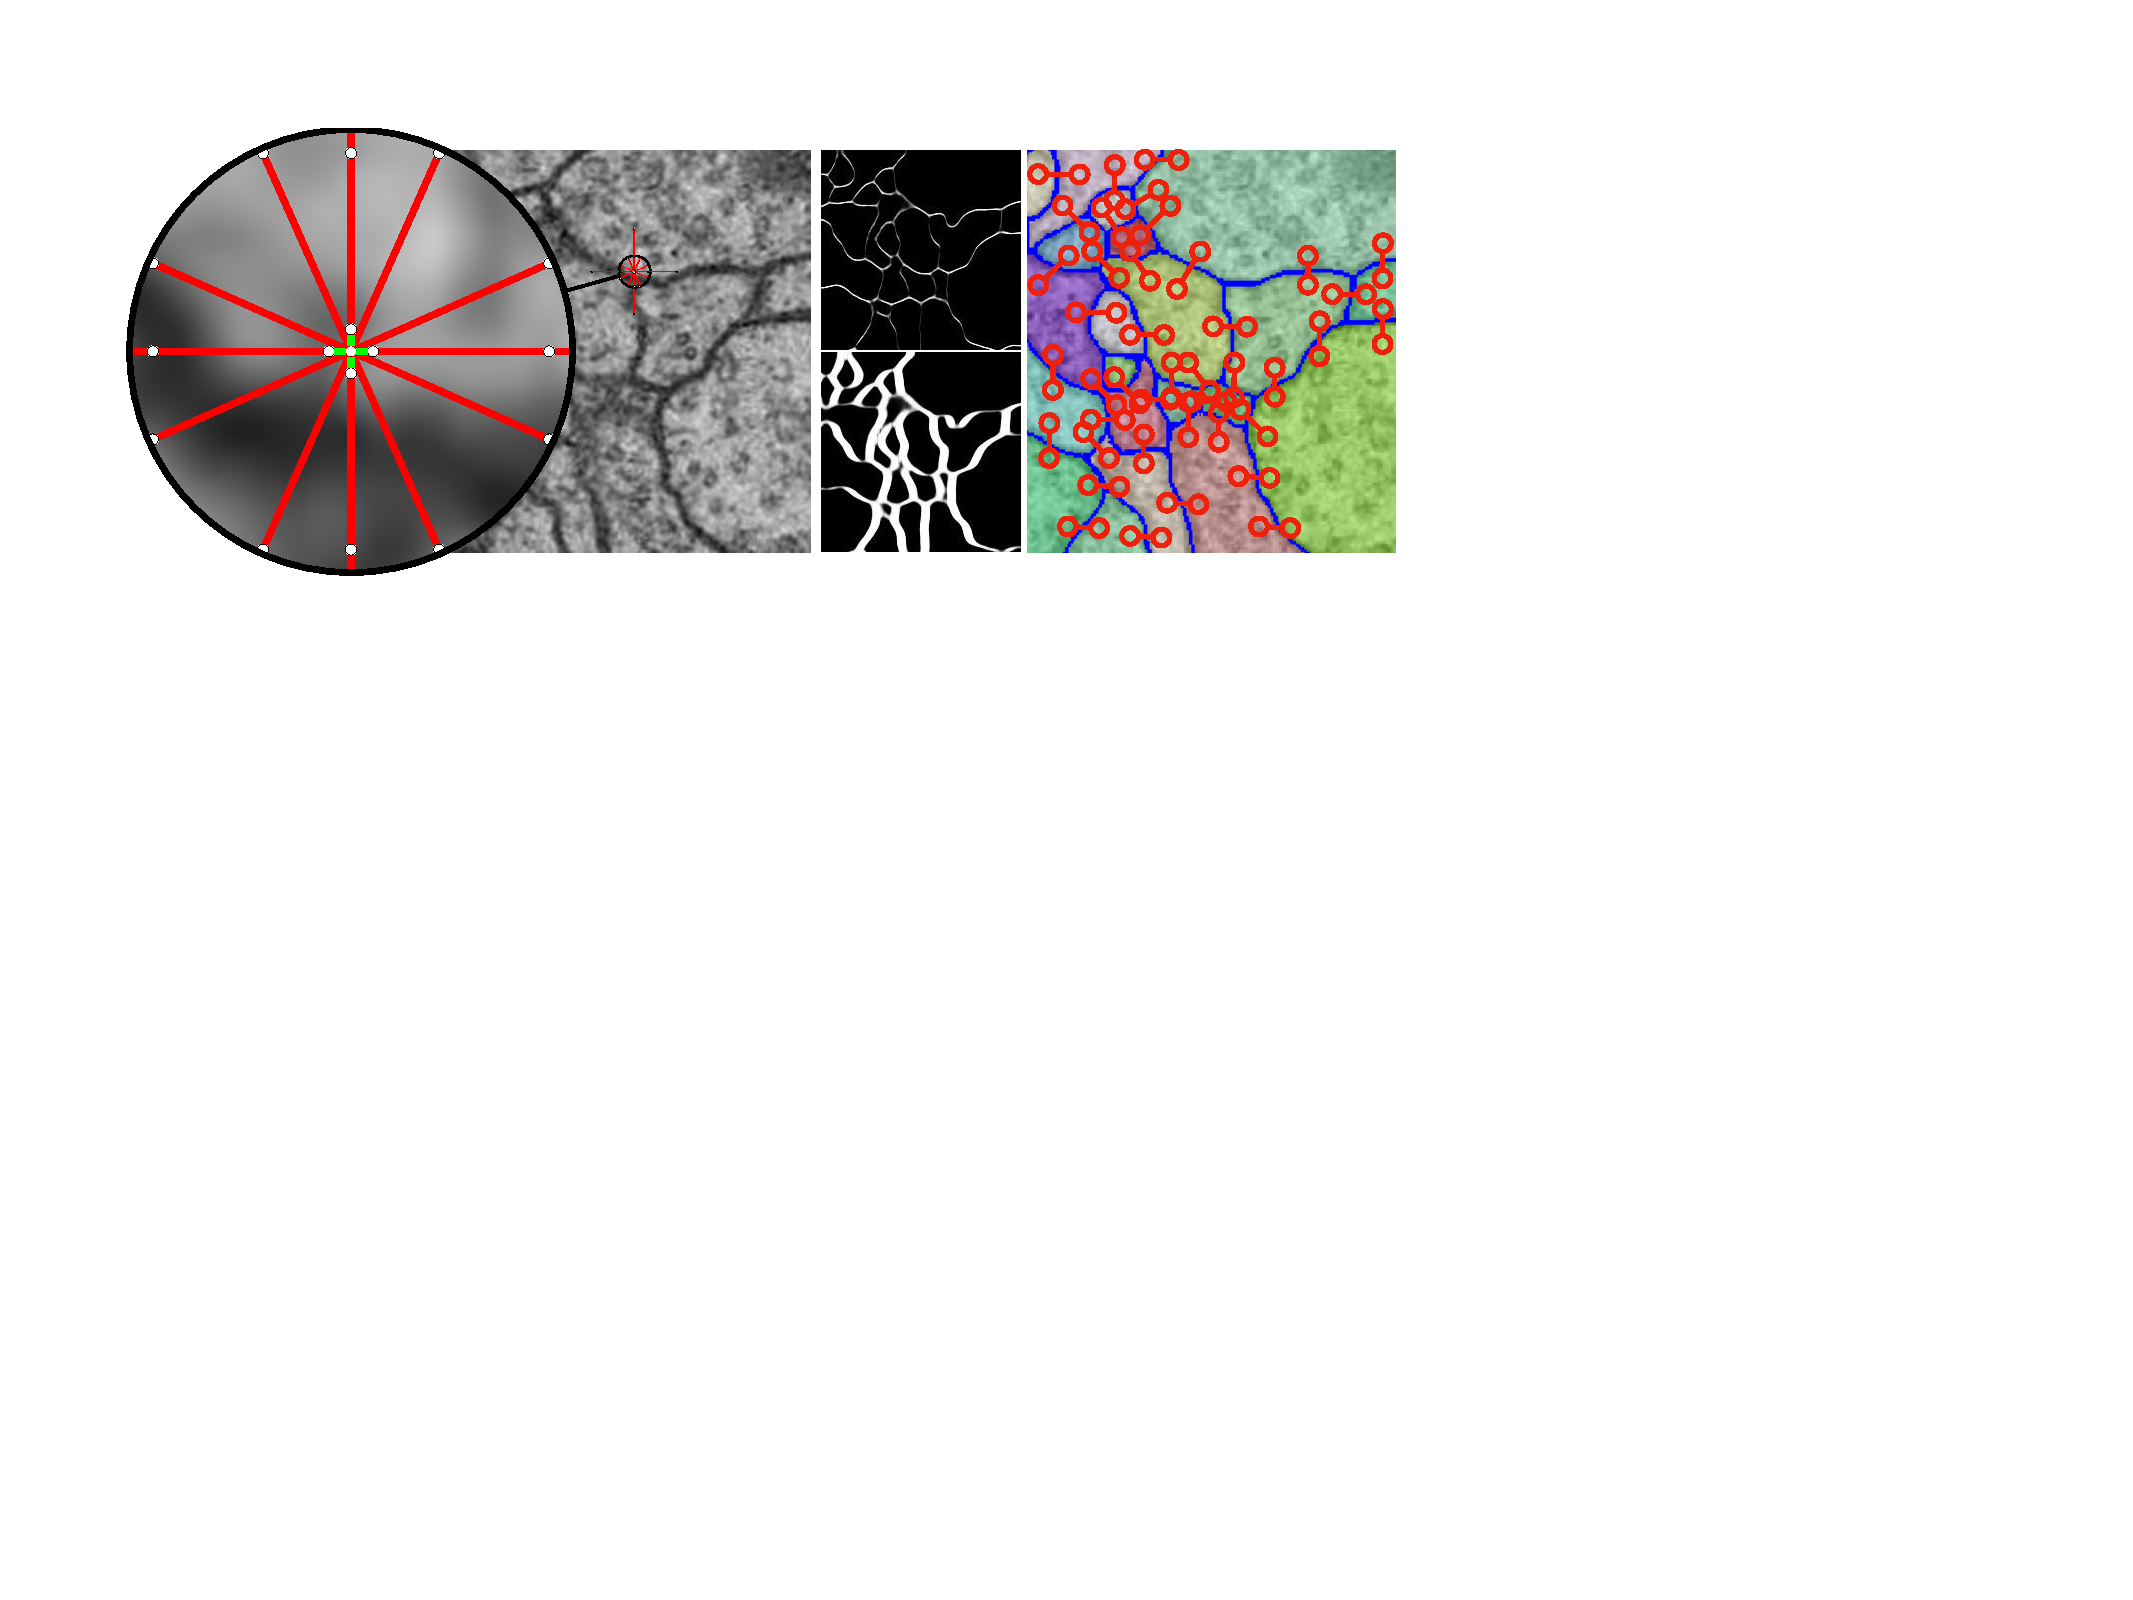
\includegraphics[width=1.\linewidth]{figures/MWS/images/fig1slimt.pdf}%
    % \begin{tabular}{cc}
    % \includegraphics[width=0.1\linewidth, valign=t]{images/affp0p0p-1pzp6.jpg}%
    % \includegraphics[width=0.1\linewidth, valign=t]{images/affp0p-9p0pzp6.jpg}\\
    % \includegraphics[width=0.1\linewidth, valign=t]{images/affp-1p1p-1pzp6.jpg}%
    % \includegraphics[width=0.1\linewidth, valign=t]{images/affp0p0p-9.jpg}\\   
    % \end{tabular}
    % \includegraphics[width=0.2\linewidth, valign=t]{images/affp0p0p-9.jpg}
    % \includegraphics[width=0.3\linewidth]{images/U-Net.pdf}%
    % \includegraphics[width=0.3\linewidth, valign=t]{images/fig_1_seg.png}
    \caption{Left: Overlay of raw data from the ISBI 2012 EM segmentation challenge and the edges for which attractive (green) or repulsive (red) interactions are estimated for each pixel using a CNN. Middle: vertical / horizontal repulsive interactions at intermediate / long range are shown in the top / bottom half. Right: Active mutual exclusion (mutex) constraints that the proposed algorithm invokes during the segmentation process.}
    \label{fig:main}
    \vspace{-0.05cm}
\end{figure}


% !TEX root = ../../main.tex

\section{Related Work} \label{2_rel_work}

\noindent In the original watershed algorithm \cite{vincent1991watersheds,Beucher-Lantu-79}, seeds were automatically placed at all local minima of the boundary map. Unfortunately, this leads to severe over-segmentation. Defining better seeds has been a recurring theme of watershed research ever since. The simplest solution is offered by the seeded watershed algorithm \cite{beucher1992morphological}: It relies on an oracle (an external algorithm or a human) to provide seeds and assigns each pixel to its nearest seed in terms of minimax path distance.

\REVIEW{In the absence of an oracle, many automatic methods for seed selection have been proposed in the last decades with applications in the fields of medicine and biology. Many of these approaches rely on edge feature extraction and edge detection like gradient calculation \cite{pohle2001segmentation,alattar2010myocardial}. Other types of methods generate seeds by first performing feature extraction \cite{poonguzhali2006complete,wu2008texture}, whereas others first extract region of interests and then place seeds inside these regions by using thresholding \cite{al2014computer}, binarization \cite{shan2008novel}, $k$-means \cite{mubarak2012hybrid} or other strategies \cite{abdelsamea2011enhancement,al2014breast}. 
% In this work seeds are interpreted as mutual exclusion constraints and the presented algorithm, that selects these constraints to form clusters can therefore be seen as a complementary approach to seed selection.
}

\REVIEW{In applications where the number of regions is hard to estimate, simple automatic seed selection methods, e.g.\ defining seeds by connected regions of low boundary probability, don't work: The segmentation quality is usually insufficient because multiple seeds are in the same region and/or seeds leak through the boundary.} Thus, in these cases seed selection may be biased towards over-seg\-men\-ta\-tion (with seeding at all minima being the extreme case). The watershed algorithm then produces superpixels that are merged into final regions by more or less elaborate postprocessing. This works better than using watersheds alone because it exploits the larger context afforded by superpixel adjacency graphs. Many criteria have been proposed to identify the regions to be preserved during merging, e.g.\ region dynamics \cite{grimaud_92_watershed-dynamics}, the waterfall transform \cite{beucher1994watershed}, extinction values \cite{vachier1995extinction}, region saliency \cite{najman1996geodesic}, and $(\alpha,\omega)$-connected components \cite{soille_08_hierarchical-image-decomposition}. A merging process controlled by criteria like these can be iterated to produce a hierarchy of segmentations where important regions survive to the next level. Variants of such hierarchical watersheds are reviewed and evaluated in \cite{perret_17_hierarchical-watersheds}.

These results highlight the close connection of watersheds to hierarchical clustering and minimum spanning trees/forests \cite{meyer1999morphological,najman_11_ultrametric-watersheds}, which inspired novel merging strategies and termination criteria. For example, \cite{salembier_00_binary-partition-tree} simply terminated hierarchical merging by fixing the number of surviving regions beforehand. \cite{malmberg2011generalized} incorporate predefined sets of generalized merge constraints into the clustering algorithm. Graph-based segmentation according to \cite{felzenszwalb_04_graph-based-image-segmentation} defines a measure of quality for the current regions and stops when the merge costs would exceed this measure. Ultrametric contour maps \cite{arbelaez_11_gpb} combine the gPb (global probability of boundary) edge detector with an oriented watershed transform. Superpixels are agglomerated until the ultrametric distance between the resulting regions exceeds a learned threshold. An optimization perspective is taken in \cite{kiran_13_hierarchical-cuts,guigues2006scale}, which introduces $h$-increasing energy functions and builds the hierarchy incrementally such that merge decisions greedily minimize the energy. The authors prove that the optimal cut corresponds to a different unique segmentation for every value of a free regularization parameter.

\REVIEW{An important line of research is given by partitioning of graphs with both attractive and repulsive edges \cite{keuper2016multi}.} Solutions that optimally balance attraction and repulsion do not require external stopping criteria such as predefined number of regions or seeds. This generalization leads to the NP-hard problem of correlation clustering or (synonymous) multicut (MC) partitioning. Fortunately, modern integer linear programming solvers in combination with incremental constraint generation can solve problem instances of considerable size \cite{andres_12_globally}, and good approximations exist for even larger problems \cite{yarkony2012fast,pape2017solving}
Reminiscent of strict minimizers \cite{Levi} with minimal $L_\infty$-norm solution, our work solves the multicut objective optimally when all graph weights are raised to a large power.


% In the limit that transforms the multicut objective into the Mutex Watershed objective, the strongest edge along a given cut is dominant by construction; an observation that
% hints at a different approach to proving the optimality of the Mutex Watershed for its objective.

% When we consider the MC as an $L_1$ minimization problem the $p \rightarrow \infty$


% . In geometric optimization strict minimizers, are the limit of $L_p$-norm minimizers for $p \rightarrow \infty$,  \cite{Levi}. We show that mc can be efficitently solved in the $p \rightarrow \infty$ limit.


% $p$-norm, for $p \rightarrow \infty$ $L_1$-norm of all cut energies minimal $L_{\infty}$-norm solution similar to strict minimizer

Related to the proposed method, the greedy additive edge contraction (GAEC) \cite{keuper2015efficient} heuristic for the multicut also sequentially merges regions, but we handle attractive and repulsive interactions separately and define edge strength between clusters by a maximum instead of an additive rule.
The greedy fixation algorithm introduced in \cite{levinkov2017comparative} is closely related to the proposed method; it sorts attractive and repulsive edges by their absolute
weight, merges nodes connected by attractive edges and introduces no-merge constraints
for repulsive edges. However, similar to GAEC, it defines edge strength by an additive rule,
which increases the algorithm's runtime complexity compared to the presented Mutex Watershed. Also, it is not yet known what objective the algorithm optimizes globally, if any.

Another beneficial extension is the introduction of additional long-range edges. The strength of such edges can often be estimated with greater certainty than is achievable for the local edges used by watersheds on standard 4- or 8-connected pixel graphs. Such repulsive long-range edges have been used in \cite{zhang_14_cell} to represent object diameter constraints, which is still an MC-type problem. When long-range edges are also allowed to be attractive, the problem turns into the more complicated lifted multicut (LMC) \cite{horvnakova2017analysis}. Realistic problem sizes can only be solved approximately \cite{keuper2015efficient,beier2016efficient}, but watershed superpixels followed by LMC postprocessing achieve state-of-the-art results on important benchmarks \cite{beier2017multicut}. Long-range edges are also used in \cite{lee2017superhuman}, as side losses for the boundary detection convolutional neural network~(CNN); but they are not used explicitly in any downstream inference.

In general, striking progress in watershed-based segmentation has been achieved by learning boundary maps with CNNs. This is nicely illustrated by the evolution of neurosegmentation for connectomics, an important field we also address in the experimental section. CNNs were introduced to this application in \cite{jain2007supervised} and became, in much refined form \cite{ciresan_12_deep-em-segmentation}, the winning entry of the ISBI 2012 Neuro-Segmentation Challenge \cite{isbi2012challenge}. Boundary maps and superpixels were further improved by progress in CNN architectures and data augmentation methods, using U-Nets \cite{ronneberger_15_u-net}, FusionNets \cite{quan2016fusionnet} or inception modules \cite{beier2017multicut}. Subsequent postprocessing with the GALA algorithm \cite{GALA,knowles2016rhoananet}, conditional random fields \cite{uzunbacs_14_optree} or the lifted multicut \cite{beier2017multicut} pushed the envelope of final segmentation quality. MaskExtend \cite{meirovitch2016multi} applied CNNs to both boundary map prediction and superpixel merging, while flood-filling networks \cite{floodfill} eliminated superpixels altogether by training a recurrent neural network to perform region growing one region at a time.

Most networks mentioned so far learn boundary maps on pixels, but learning works equally well for edge-based watersheds, as was demonstrated in \cite{zlateski2015image,parag2017anisotropic} using edge weights generated with a CNN \cite{turaga2010convolutional,MALIS}. Tayloring the learning objective to the needs of the watershed algorithm by penalizing critical edges along minimax paths \cite{MALIS} or end-to-end training of edge weights and region growing \cite{wolf2017learned} improved results yet again.

Outside of connectomics, \cite{bai2016deep_watershed} obtained superior boundary maps from CNNs by learning not just boundary strength, but also its gradient direction. Holistically-nested edge detection \cite{xie2015holistically,kokkinos2015pushing} couples the CNN loss at multiple resolutions using deep supervision and is successfully used as a basis for watershed segmentation of medical images in \cite{cai2016pancreas}. 

We adopt important ideas from this prior work (hierarchical single-linkage clustering, attractive and repulsive interactions, long-range edges, and CNN-based learning). The proposed efficient segmentation framework can be interpreted as a generalization of \cite{malmberg2011generalized}, because we also allow for soft repulsive interactions (which can be overridden by strong attractive edges), and constraints are generated on-the-fly.

%!TEX root = ../../main.tex

% \cleardoublepage




\section{The Mutex Watershed Algorithm as an Extension of Seeded Watershed} \label{3_methods}
In this section we introduce the Mutex Watershed Algorithm, an efficient graph clustering algorithm that can ingest both attractive and repulsive cues. We first reformulate seeded watershed as a graph partitioning with infinitely repulsive edges and then derive the generalized algorithm for finitely repulsive edges, which obviates the need for seeds.


\subsection{Definitions and notation}\label{sec:notation}
Let $\mathcal{G}=(V, E, w)$ be a weighted graph. 
% \TODO{Why do we need this here? (also $\Pi$ is used for paths and partitions)\\
% We call a partition $\Pi$ of
% $V$ a clustering if every $S \in \Pi$ induces a connected subgraph
% (cluster) of $G .$ For any clustering $\Pi$ of $G,$ we denote by $E_{\Pi}^{0}$
% the set of those edges whose nodes are in the same cluster,
% and by $E_{\Pi}^{1}$ the (complementary) set of those edges whose nodes are in distinct clusters:
% \begin{align}
% E_{\Pi}^{0} &=\{u v \in E | \exists S \in \Pi : u \in S \text { and } v \in S\} \\
% E_{\Pi}^{1} &=E \backslash E_{\Pi}^{0}
% \end{align}
% The set of edges $E_{\Pi}^{1}$ is known as the multicut of $G$ that corresponds to the clustering $\Pi$.}
The scalar attribute $w : E \rightarrow \mathbb{R}$ associated with each edge is a merge affinity: the higher this number, the higher the inclination of the two incident vertices to be assigned to the same cluster. Conversely, large negative affinity indicates a greater desire of the incident vertices to be in different clusters. In our application, each vertex corresponds to one pixel in the image to be segmented. 
We call an edge $e \in E$ repulsive if $w_{e}<0$ and we call it attractive if $w_{e}>0$ 
% Note that we may w.l.o.g. remove all edges $e \in E$ with $w_{e}=0,$ since the choice of $x_{e}$ is irrelevant to the objective. 
and collect them in $E^{-} = \{  e \in E \,|\, w_e < 0 \}$ and $E^{+} = \{ e \in E \; | \; w_e > 0 \}$ respectively.

In our application, each vertex corresponds to one pixel in the image to be segmented. 
% \REVIEW{\sout{Edges can be either {\it local/short-range} (when connecting two pixels that are immediately adjacent in the image) or {\it long-range}.}}
% Our algorithm ``activates'' attractive edges to merge and introduces mutual exclusion relations by ``activating'' repulsive edges. Given the ``active'' subset $A^+ \subseteq E^+$ of attractive edges, clusters are defined via the ``connected'' predicate: 
The Mutex Watershed algorithm, defined in \autoref{3_3_MWS}, maintains disjunct active sets $A^+ \subseteq E^+$, $A^- \subseteq E^-$, $A^+ \cap A^- = \emptyset$ that encode merges and mutual exclusion constraints, respectively. Clusters are defined via the ``connected'' predicate: %
\begin{eqnarray*}
\forall i,j\in V:\\
\Pi_{i \rightarrow j} & = & \{ \text{paths } \pi\text{ from }i\text{ to }j\text{ with }\pi\subseteq E^+\}\\
\operator{connected}(i, j; A^+)&\Leftrightarrow& \exists \text{ path } \pi \in \Pi_{i \rightarrow j} \text{ with }\pi \subseteq A^+ \\
\operator{cluster}(i; A^+) & = & \{i\} \cup \{j: \operator{connected}(i,j; A^+) \}
\end{eqnarray*}
Conversely, the active subset $A^-\subseteq E^-$ of repulsive edges defines mutual exclusion relations by using the following predicate: % is defined in terms of active repulsive edges $A^-$ as
\begin{eqnarray*}
\operator{mutex}(i, j; A^+, A^-)&\Leftrightarrow& \exists \, e=(k,l)\in A^- \text{ with } \\ && k \in \operator{cluster}(i; A^+) \text{ and}\\
& & l \in \operator{cluster}(j; A^+) \text{ and} \\
&&\operator{cluster}(i; A^+) \neq \operator{cluster}(j; A^+)
\end{eqnarray*}
Admissible active edge sets $A^+$ and $A^-$ must be chosen such that the resulting clustering is consistent, i.e.\ nodes engaged in a mutual exclusion constraint cannot be in the same cluster:
$\operator{mutex}(i,j; A^+, A^-) \Rightarrow \operator{not} \:\: \operator{connected}(i, j; A^+)$.
The ``connected'' and ``mutex'' predicates can be efficiently evaluated using a union find data structure.

\begin{figure}[t]
\centering
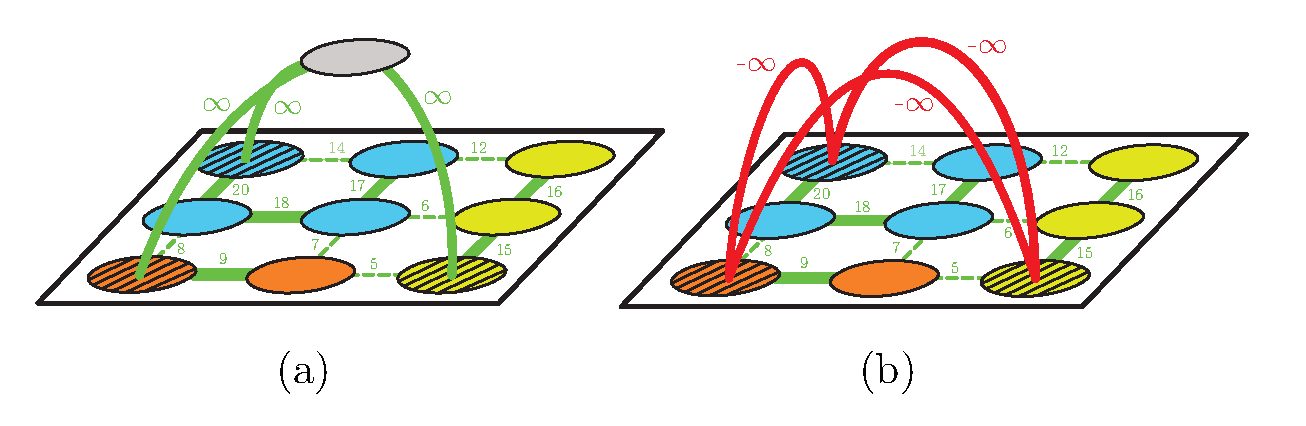
\includegraphics[width=\linewidth]{figures/MWS/images/seeded-WS.pdf}%
   %\includegraphics[width=0.8\linewidth]{egfigure.eps}
   \caption{Two equivalent representations of the seeded watershed clustering obtained using (a) a maximum spanning tree computation or (b) Algorithm \ref{WS_algo_code}. Both graphs share the weighted attractive~(green) edges and seeds (hatched nodes). The infinitely attractive connections to the auxiliary node (gray) in (a) are replaced by infinitely repulsive~(red) edges between each pair of seeds in (b). The two final clusterings are defined by the active sets (bold edges) and are identical. Node colors indicate the clustering result, but are arbitrary.}
\label{fig:WS_compare}
\end{figure}




\begin{algorithm}[t]
  \caption{Mutex version of seeded watershed algorithm}

  \begin{algorithmic}[1]
      \Procedure{SeededWatershed}{$\mathcal{G}(V,E),$ \text{\rm pos.\ weights} $w:E\rightarrow \mathbb  {R}^+$, \text{\rm seeds} $S\subseteq V$}
        \State $A^+ \leftarrow \emptyset$\; 
        \State $A^- \leftarrow \{ (s,t) \in S \times S \,|\, s \neq t \} $ % \Comment{Equiv. to adding infinitely repulsive edges between seeds}
        \For{$(i,j) = e \in E $ {\rm in descending order of } $w_e$} 
            \If{\rm {\bf not} $\operator{connected}$($i, j; A^+$) \textbf{and not} $\operator{mutex}$($i,j;A^+,A^-$) }  
                \State $A^+ \leftarrow A^+ \cup e$ \Comment{Merge $i,j$ and inherit mutex constraints of the parent clusters}
            \EndIf
        \EndFor
        \State
        \Return $A^+ \cup A^-$
      \EndProcedure
  \end{algorithmic}
    \algcomment{The output clustering is defined by the connected components of the final attractive active set $A^+$.}
 \label{WS_algo_code}
\end{algorithm}


\subsection{Seeded watershed from a mutex perspective}
\noindent One interpretation of the proposed method is in terms of a generalization of the edge-based watershed algorithm \cite{Meyer1994,Meyer1994minimum,meyer1999morphological}
 or image foresting transform \cite{falcao2004image}.
This algorithm can only ingest a graph with purely attractive interactions, $E^{-} = \emptyset$. Without  further constraints, the algorithm would yield only the trivial result of a single cluster comprising all vertices. To obtain more interesting output, an oracle needs to provide seeds~(e.g.\ one node per cluster). These seed vertices are all connected to an auxiliary node (see Fig.~\ref{fig:WS_compare} (a)) by auxiliary edges with infinite merge affinity. A maximum spanning tree (MST) on this augmented graph can be found in linearithmic time; and the maximum spanning tree (or in the case of degeneracy: at least one of the maximum spanning trees) will include the auxiliary edges. When the auxiliary edges are deleted from the MST, a forest results, with each tree representing one cluster \cite{meyer1999morphological,Meyer1994,falcao2004image}.

We now reformulate this well-known algorithm in a way that will later emerge as a special case of the proposed Mutex Watershed: 
we eliminate the auxiliary node and edges, and replace them by a set of infinitely repulsive edges, one for each pair of seeds (Fig.~\ref{fig:WS_compare} (b)).
Algorithm \ref{WS_algo_code} is a variation of Kruskal's MST algorithm operating on the seed mutex graph just defined, and gives results identical to seeded watershed on the original graph. 


This algorithm differs from Kruskal's only by the check for mutual exclusion in the if-statement. Obviously, the modified algorithm has the same effect as the original algorithm, because the final set $A^+$ is exactly the maximum spanning forest obtained after removing the auxiliary edges from the original solution. 

In the sequel, we generalize this construction by admitting less-than-infinitely repulsive edges. Importantly, these can be dense and are hence much easier to estimate automatically than seeds with their strict requirement of only-one-per-cluster.










\begin{algorithm}[t]
 % \hrulefill \\
  \caption{Mutex Watershed Algorithm}
  \begin{algorithmic}[1]
    \Procedure{MutexWatershed}{$\mathcal{G}(V,E)$, $w:E\rightarrow \mathbb{R}$, \text{\rm boolean $\operator{connect\_all}$}}
        \State $A^+ \leftarrow \emptyset; \quad A^- \leftarrow \emptyset $\;
        \For{$(i,j) = e \in E $ {\rm in descending order of } $|w_e|$} 
            \If{$e \in E^+$}
                \If{\rm \textbf{not} $\operator{mutex}$($i,j; A^+, A^-$) }  
                    \If{\rm {\bf not} $\operator{connected}$($i, j; A^+$) \textbf{or} \rm $\operator{connect\_all}$}
                        \State $\operator{merge}(i, j)$: $A^+ \leftarrow A^+ \cup e$
                        \Comment{Merge $i, j$ and inherit constraints of parent clusters}
                    \EndIf
                \EndIf
           \Else
                \If{\rm {\bf not} $\operator{connected}$($i, j; A^+$)}
                    \State $\operator{addmutex}(i, j)$: $A^- \leftarrow A^- \cup e$\;
                    \Comment{Add mutex constraint between $i$ and $j$}
                \EndIf
            \EndIf
        \EndFor
        \State 
        \Return $A^+ \cup A^-$
    \EndProcedure
    \end{algorithmic}
 \label{algo_code_efficient}
 \algcomment{\REVIEW{The output clustering is defined by the connected components of the final attractive active set $A^+$. The $\operator{connect\_all}$ parameter changes the internal cluster connectedness from trees to fully connected, but does not change the output clustering.} The $\operator{connected}$ predicate can be efficiently evaluated using union find data structures.}
% }
\end{algorithm}





\begin{figure}[htp]
\centering
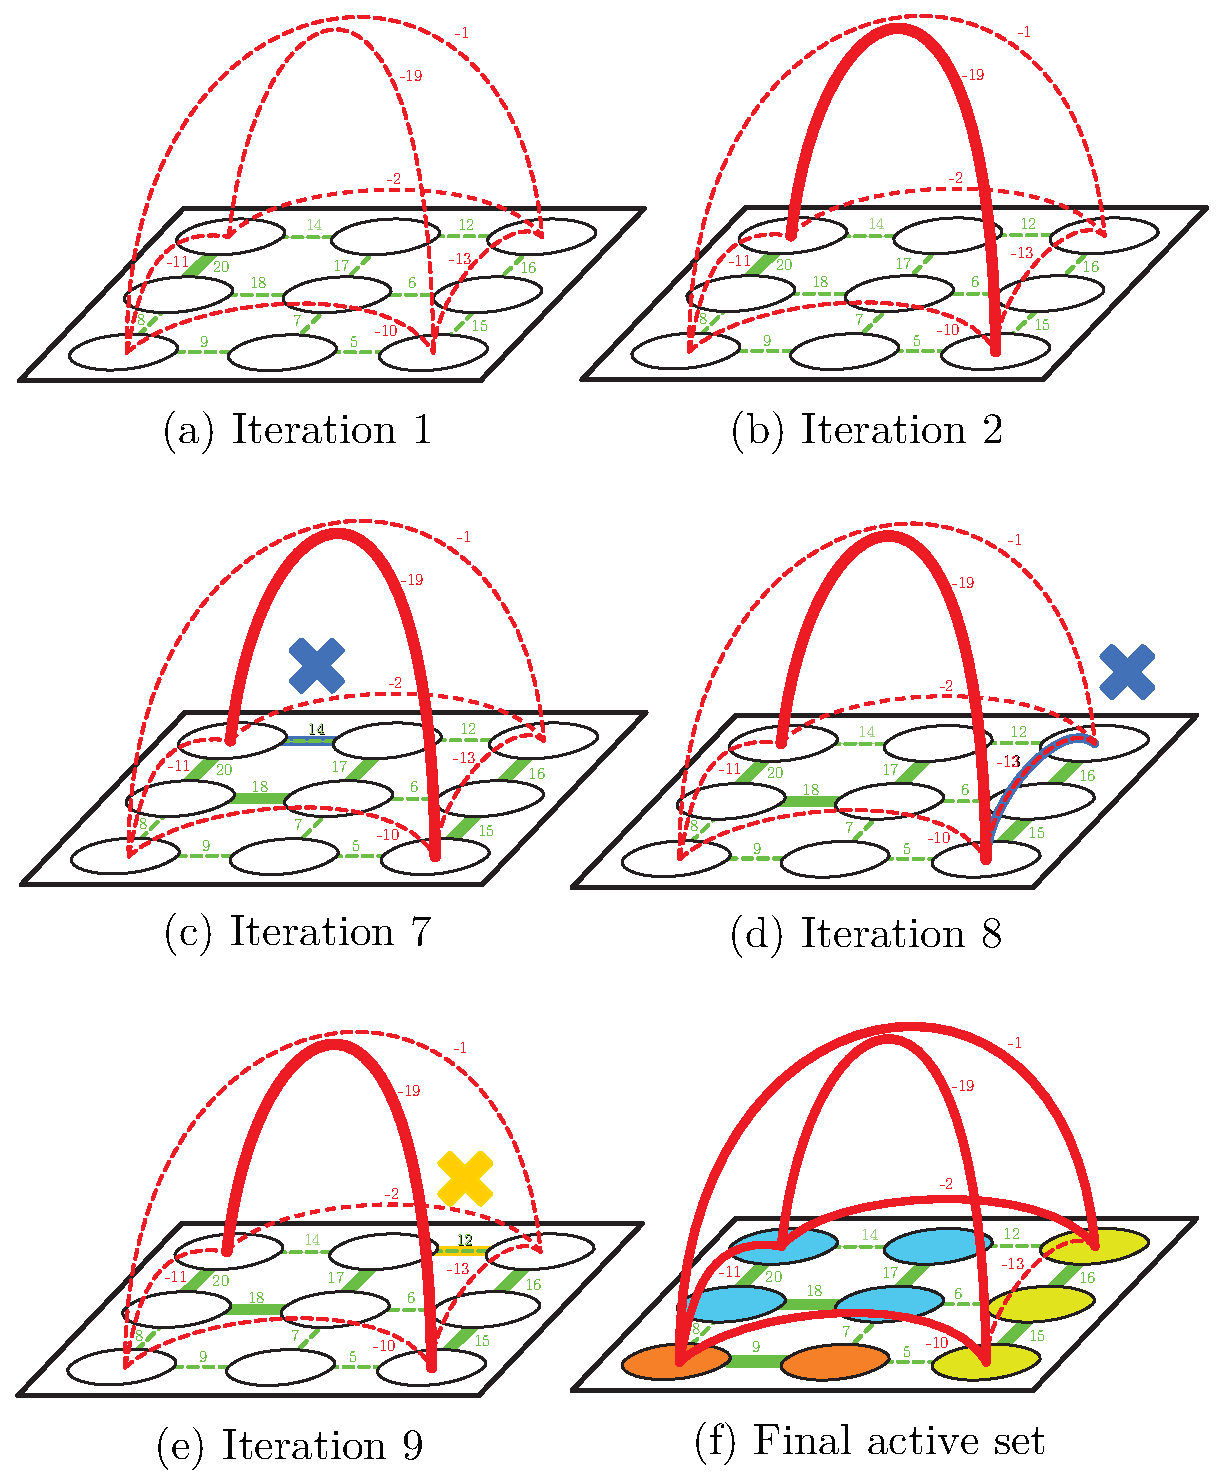
\includegraphics[width=0.9\linewidth]{figures/MWS/images/new-diagram-MWS-2.pdf}
% \includegraphics[width=\linewidth]{images/exampleg1.png}
% \includegraphics[width=\linewidth]{images/exampleg2.png}
   %\includegraphics[width=0.8\linewidth]{egfigure.eps}
   \caption{Some iterations of the Mutex Watershed Algorithm \ref{algo_code_efficient} applied to a graph with weighted attractive (green) and repulsive (red) edges. Edges accumulated in the active set $A$ after a given number of iterations are shown in bold. \REVIEW{The $\operator{connect\_all}$ parameter of the algorithm is set to $\operator{False}$, so that only the positive edges belonging to the maximum spanning tree of each cluster are added to the active set.} Once the algorithm terminates, the final active set (f) defines the final clustering (indicated using arbitrary node colors). Some edges are not added to the active set because they are mutex constrained~(yellow highlight) or because the associated nodes are already connected and in the same cluster~(blue highlight).}
   %Some edges that are not added to the active set because they would violate constraints $\mathcal{C}_{0}$ or $\mathcal{C}_{1}$ are highlighted in blue and yellow, respectively. \TODO{Update}}
\label{fig:MWS_algorithm}
\end{figure}

\subsection{Mutex Watersheds}\label{3_3_MWS}

\noindent 
We now introduce our core contribution: an algorithm that is empirically no more expensive than a MST computation; but that can ingest both attractive and repulsive cues and partition a graph into a number of clusters that does not need to be specified beforehand. \REVIEW{Neither seeds nor hyperparameters that implicitly determine the number of resulting clusters are required.}

The Mutex Watershed, Algorithm \ref{algo_code_efficient}, proceeds as follows. Given a graph $\mathcal{G}=(V, E)$ with signed weights $w: E \rightarrow \mathbb{R}$, do the following: sort all edges $E$, attractive or repulsive, by their absolute weight in descending order into a priority queue. Iteratively pop all edges from the queue and add them to the active set one by one, provided that a set of conditions are satisfied.
More specifically, assuming $\operator{connect\_all}$ is $\operator{False}$, if the next edge popped from the priority queue is attractive and its incident vertices are not yet in the same tree, then connect the respective trees provided this is not ruled out by a mutual exclusion constraint. If on the other hand the edge popped is repulsive, and if its incident vertices are not yet in the same tree, then add a mutual exclusion constraint between the two trees. 
The output clustering is defined by the connected components of the final attractive active set $A^+$.

 The crucial difference to Algorithm \ref{WS_algo_code} is that mutex constraints are no longer pre-defined, but created dynamically whenever a repulsive edge is found. However, new exclusion constraints can never override earlier, high-priority merge decisions. In this case, the repulsive edge in question is simply ignored. Similarly, an attractive edge must never override earlier and thus higher-priority must-not-link decisions. 

\REVIEW{The boolean value of the $\operator{connect\_all}$ input parameter of the algorithm does not influence the final output clustering, but defines the internal cluster connectedness: when it is set to $\operator{True}$, the algorithm adds all attractive intra-cluster edges to the active set $A^+$. When it is set to $\operator{False}$, then a maximum spanning tree is built for each cluster similarly to the seeded watershed. This variant of the algorithm will be helpful in the next section \ref{sec:MWS_objective} to highlight the relation between the Mutex Watershed and the multicut problem.}
% \TODO{Mention correctness, guaranteed termination?}

Fig. \ref{fig:MWS_algorithm} illustrates the proposed algorithm: Fig. \ref{fig:MWS_algorithm}a and Fig. \ref{fig:MWS_algorithm}b show examples of an unconstrained merge and an added mutex constraint, respectively; Fig. \ref{fig:MWS_algorithm}c and Fig. \ref{fig:MWS_algorithm}d show, respectively, an example of an attractive edge ($w_e=14$) and repulsive edge ($w_e=-13$) that are not added to the active set because their incident vertices  are already ``connected'' and belong to the same tree of the forest $A^+$; finally, Fig. \ref{fig:MWS_algorithm}e shows an attractive edge ($w_e=12$) that is ruled out by a previously introduced mutual exclusion relation.


\subsection{Time Complexity Analysis}


Before analyzing the time complexity of algorithm \ref{algo_code_efficient} we first review the complexity of Kruskal's algorithm. Using a union-find data structure~(with path compression and union by rank) the time complexity of $\operator{merge}(i,~j)$ and $\operator{connected}(i,~j)$ is $\mathcal{O}(\alpha(V))$, where $\alpha$ is the slowly growing inverse Ackerman function, and the total runtime complexity is dominated by the initial sorting of the edges $\mathcal{O}(E \log E)$\cite{cormen2009introduction}.

\noindent To check for mutex constraints efficiently, we maintain a set of all active mutex edges $$ M[C_i] = \{(u,~v) \in A^- | u \in C_i \lor v \in C_i\} $$ for every $C_i = \operator{cluster}(i)$ using hash tables, where insertion of new mutex edges~(i.e. $\operator{addmutex}$) and search have an average complexity of $\mathcal{O}(1)$. Note that every cluster can be efficiently identified by its union-find root node.
For $\operator{mutex}(i,~j)$ we check if $M[C_i] \cap M[C_j] = \emptyset$ by searching for all elements of the smaller hash table in the larger hash table. Therefore $\operator{mutex}(i,~j)$ has an average complexity of $\mathcal{O}(\min (|M[C_i]|, |M[C_j]|)$. % and a worst case complexity of $\mathcal{O}(|M[C_i]|\cdot|M[C_j]|)$.
Similarly, during $\operator{merge}(i,~j)$, mutex constraints are inherited  by merging two hash tables, which also has an average complexity $\mathcal{O}(\min (|M[C_i]|, |M[C_j]|)$. 

\noindent In conclusion, the average runtime contribution of attractive edges $\mathcal{O}(\max(|E^{+}| \cdot\alpha(V), |E^{+}| \cdot M))$ (checking mutex constraints and possibly merging) and repulsive edges
 $\mathcal{O}(\max(|E^{-}| \cdot \alpha(V), |E^{-}|)) $ (insertion of one mutex edge) result in a total average runtime complexity of algorithm \ref{algo_code_efficient}:
 \vspace{-0.1cm}
    % \begin{equation}
    %     \mathcal{O}(E \log E + E  \cdot  \alpha(V) + EM).
    % \end{equation}
    \begin{equation}
         \mathcal{O}(\max(E \log E \;,\; EM)).
    \end{equation}
where $M$ is the expected value of $\min (|M[C_i]|, |M[C_j]|)$ and $\alpha(V) \in \mathcal{O}(\log V) \in \mathcal{O}(\log E) $ \footnote{In the worst case $G$ is a fully connected graph, with $|E|=|V|^2$, hence $\log |V| = \frac{1}{2} \log |E|$.}.


\noindent In the worst case $\mathcal{O}(M) \in \mathcal{O}(E)$, the Mutex Watershed Algorithm has a runtime complexity of  $\mathcal{O}(E^2)$. Empirically, we find that $\mathcal{O}(EM) \approx \mathcal{O}(E\log E)$ by measuring the runtime of Mutex Watershed for different sub-volumes of the ISBI challenge~(see Figure \ref{fig:scalingM}), leading to a 
\begin{equation}
    \text{Empirical Mutex Watershed Complexity: }\mathcal{O}(E \log E)
\end{equation}


\begin{figure}[ht]
   \centering
\adjustbox{width=0.88\linewidth}{
       %% Creator: Matplotlib, PGF backend
%%
%% To include the figure in your LaTeX document, write
%%   \input{<filename>.pgf}
%%
%% Make sure the required packages are loaded in your preamble
%%   \usepackage{pgf}
%%
%% Figures using additional raster images can only be included by \input if
%% they are in the same directory as the main LaTeX file. For loading figures
%% from other directories you can use the `import` package
%%   \usepackage{import}
%% and then include the figures with
%%   \import{<path to file>}{<filename>.pgf}
%%
%% Matplotlib used the following preamble
%%   \usepackage{fontspec}
%%   \setmainfont{DejaVu Serif}
%%   \setsansfont{DejaVu Sans}
%%   \setmonofont{DejaVu Sans Mono}
%%
\begingroup%
\makeatletter%
\begin{pgfpicture}%
\pgfpathrectangle{\pgfpointorigin}{\pgfqpoint{7.000000in}{7.000000in}}%
\pgfusepath{use as bounding box, clip}%
\begin{pgfscope}%
\pgfsetbuttcap%
\pgfsetmiterjoin%
\definecolor{currentfill}{rgb}{1.000000,1.000000,1.000000}%
\pgfsetfillcolor{currentfill}%
\pgfsetlinewidth{0.000000pt}%
\definecolor{currentstroke}{rgb}{1.000000,1.000000,1.000000}%
\pgfsetstrokecolor{currentstroke}%
\pgfsetdash{}{0pt}%
\pgfpathmoveto{\pgfqpoint{0.000000in}{0.000000in}}%
\pgfpathlineto{\pgfqpoint{7.000000in}{0.000000in}}%
\pgfpathlineto{\pgfqpoint{7.000000in}{7.000000in}}%
\pgfpathlineto{\pgfqpoint{0.000000in}{7.000000in}}%
\pgfpathclose%
\pgfusepath{fill}%
\end{pgfscope}%
\begin{pgfscope}%
\pgfsetbuttcap%
\pgfsetmiterjoin%
\definecolor{currentfill}{rgb}{0.917647,0.917647,0.949020}%
\pgfsetfillcolor{currentfill}%
\pgfsetlinewidth{0.000000pt}%
\definecolor{currentstroke}{rgb}{0.000000,0.000000,0.000000}%
\pgfsetstrokecolor{currentstroke}%
\pgfsetstrokeopacity{0.000000}%
\pgfsetdash{}{0pt}%
\pgfpathmoveto{\pgfqpoint{0.875000in}{0.770000in}}%
\pgfpathlineto{\pgfqpoint{6.300000in}{0.770000in}}%
\pgfpathlineto{\pgfqpoint{6.300000in}{6.160000in}}%
\pgfpathlineto{\pgfqpoint{0.875000in}{6.160000in}}%
\pgfpathclose%
\pgfusepath{fill}%
\end{pgfscope}%
\begin{pgfscope}%
\pgfpathrectangle{\pgfqpoint{0.875000in}{0.770000in}}{\pgfqpoint{5.425000in}{5.390000in}}%
\pgfusepath{clip}%
\pgfsetroundcap%
\pgfsetroundjoin%
\pgfsetlinewidth{1.003750pt}%
\definecolor{currentstroke}{rgb}{1.000000,1.000000,1.000000}%
\pgfsetstrokecolor{currentstroke}%
\pgfsetdash{}{0pt}%
\pgfpathmoveto{\pgfqpoint{1.125582in}{0.770000in}}%
\pgfpathlineto{\pgfqpoint{1.125582in}{6.160000in}}%
\pgfusepath{stroke}%
\end{pgfscope}%
\begin{pgfscope}%
\definecolor{textcolor}{rgb}{0.150000,0.150000,0.150000}%
\pgfsetstrokecolor{textcolor}%
\pgfsetfillcolor{textcolor}%
\pgftext[x=1.125582in,y=0.638056in,,top]{\color{textcolor}\sffamily\fontsize{11.000000}{13.200000}\selectfont \(\displaystyle 10^{6}\)}%
\end{pgfscope}%
\begin{pgfscope}%
\pgfpathrectangle{\pgfqpoint{0.875000in}{0.770000in}}{\pgfqpoint{5.425000in}{5.390000in}}%
\pgfusepath{clip}%
\pgfsetroundcap%
\pgfsetroundjoin%
\pgfsetlinewidth{1.003750pt}%
\definecolor{currentstroke}{rgb}{1.000000,1.000000,1.000000}%
\pgfsetstrokecolor{currentstroke}%
\pgfsetdash{}{0pt}%
\pgfpathmoveto{\pgfqpoint{4.010989in}{0.770000in}}%
\pgfpathlineto{\pgfqpoint{4.010989in}{6.160000in}}%
\pgfusepath{stroke}%
\end{pgfscope}%
\begin{pgfscope}%
\definecolor{textcolor}{rgb}{0.150000,0.150000,0.150000}%
\pgfsetstrokecolor{textcolor}%
\pgfsetfillcolor{textcolor}%
\pgftext[x=4.010989in,y=0.638056in,,top]{\color{textcolor}\sffamily\fontsize{11.000000}{13.200000}\selectfont \(\displaystyle 10^{7}\)}%
\end{pgfscope}%
\begin{pgfscope}%
\definecolor{textcolor}{rgb}{0.150000,0.150000,0.150000}%
\pgfsetstrokecolor{textcolor}%
\pgfsetfillcolor{textcolor}%
\pgftext[x=3.587500in,y=0.434646in,,top]{\color{textcolor}\sffamily\fontsize{12.000000}{14.400000}\selectfont Total Number of Edges |E|}%
\end{pgfscope}%
\begin{pgfscope}%
\pgfpathrectangle{\pgfqpoint{0.875000in}{0.770000in}}{\pgfqpoint{5.425000in}{5.390000in}}%
\pgfusepath{clip}%
\pgfsetroundcap%
\pgfsetroundjoin%
\pgfsetlinewidth{1.003750pt}%
\definecolor{currentstroke}{rgb}{1.000000,1.000000,1.000000}%
\pgfsetstrokecolor{currentstroke}%
\pgfsetdash{}{0pt}%
\pgfpathmoveto{\pgfqpoint{0.875000in}{0.950170in}}%
\pgfpathlineto{\pgfqpoint{6.300000in}{0.950170in}}%
\pgfusepath{stroke}%
\end{pgfscope}%
\begin{pgfscope}%
\definecolor{textcolor}{rgb}{0.150000,0.150000,0.150000}%
\pgfsetstrokecolor{textcolor}%
\pgfsetfillcolor{textcolor}%
\pgftext[x=0.500088in,y=0.892132in,left,base]{\color{textcolor}\sffamily\fontsize{11.000000}{13.200000}\selectfont 0.5}%
\end{pgfscope}%
\begin{pgfscope}%
\pgfpathrectangle{\pgfqpoint{0.875000in}{0.770000in}}{\pgfqpoint{5.425000in}{5.390000in}}%
\pgfusepath{clip}%
\pgfsetroundcap%
\pgfsetroundjoin%
\pgfsetlinewidth{1.003750pt}%
\definecolor{currentstroke}{rgb}{1.000000,1.000000,1.000000}%
\pgfsetstrokecolor{currentstroke}%
\pgfsetdash{}{0pt}%
\pgfpathmoveto{\pgfqpoint{0.875000in}{1.742783in}}%
\pgfpathlineto{\pgfqpoint{6.300000in}{1.742783in}}%
\pgfusepath{stroke}%
\end{pgfscope}%
\begin{pgfscope}%
\definecolor{textcolor}{rgb}{0.150000,0.150000,0.150000}%
\pgfsetstrokecolor{textcolor}%
\pgfsetfillcolor{textcolor}%
\pgftext[x=0.500088in,y=1.684746in,left,base]{\color{textcolor}\sffamily\fontsize{11.000000}{13.200000}\selectfont 1.0}%
\end{pgfscope}%
\begin{pgfscope}%
\pgfpathrectangle{\pgfqpoint{0.875000in}{0.770000in}}{\pgfqpoint{5.425000in}{5.390000in}}%
\pgfusepath{clip}%
\pgfsetroundcap%
\pgfsetroundjoin%
\pgfsetlinewidth{1.003750pt}%
\definecolor{currentstroke}{rgb}{1.000000,1.000000,1.000000}%
\pgfsetstrokecolor{currentstroke}%
\pgfsetdash{}{0pt}%
\pgfpathmoveto{\pgfqpoint{0.875000in}{2.535397in}}%
\pgfpathlineto{\pgfqpoint{6.300000in}{2.535397in}}%
\pgfusepath{stroke}%
\end{pgfscope}%
\begin{pgfscope}%
\definecolor{textcolor}{rgb}{0.150000,0.150000,0.150000}%
\pgfsetstrokecolor{textcolor}%
\pgfsetfillcolor{textcolor}%
\pgftext[x=0.500088in,y=2.477360in,left,base]{\color{textcolor}\sffamily\fontsize{11.000000}{13.200000}\selectfont 1.5}%
\end{pgfscope}%
\begin{pgfscope}%
\pgfpathrectangle{\pgfqpoint{0.875000in}{0.770000in}}{\pgfqpoint{5.425000in}{5.390000in}}%
\pgfusepath{clip}%
\pgfsetroundcap%
\pgfsetroundjoin%
\pgfsetlinewidth{1.003750pt}%
\definecolor{currentstroke}{rgb}{1.000000,1.000000,1.000000}%
\pgfsetstrokecolor{currentstroke}%
\pgfsetdash{}{0pt}%
\pgfpathmoveto{\pgfqpoint{0.875000in}{3.328011in}}%
\pgfpathlineto{\pgfqpoint{6.300000in}{3.328011in}}%
\pgfusepath{stroke}%
\end{pgfscope}%
\begin{pgfscope}%
\definecolor{textcolor}{rgb}{0.150000,0.150000,0.150000}%
\pgfsetstrokecolor{textcolor}%
\pgfsetfillcolor{textcolor}%
\pgftext[x=0.500088in,y=3.269973in,left,base]{\color{textcolor}\sffamily\fontsize{11.000000}{13.200000}\selectfont 2.0}%
\end{pgfscope}%
\begin{pgfscope}%
\pgfpathrectangle{\pgfqpoint{0.875000in}{0.770000in}}{\pgfqpoint{5.425000in}{5.390000in}}%
\pgfusepath{clip}%
\pgfsetroundcap%
\pgfsetroundjoin%
\pgfsetlinewidth{1.003750pt}%
\definecolor{currentstroke}{rgb}{1.000000,1.000000,1.000000}%
\pgfsetstrokecolor{currentstroke}%
\pgfsetdash{}{0pt}%
\pgfpathmoveto{\pgfqpoint{0.875000in}{4.120625in}}%
\pgfpathlineto{\pgfqpoint{6.300000in}{4.120625in}}%
\pgfusepath{stroke}%
\end{pgfscope}%
\begin{pgfscope}%
\definecolor{textcolor}{rgb}{0.150000,0.150000,0.150000}%
\pgfsetstrokecolor{textcolor}%
\pgfsetfillcolor{textcolor}%
\pgftext[x=0.500088in,y=4.062587in,left,base]{\color{textcolor}\sffamily\fontsize{11.000000}{13.200000}\selectfont 2.5}%
\end{pgfscope}%
\begin{pgfscope}%
\pgfpathrectangle{\pgfqpoint{0.875000in}{0.770000in}}{\pgfqpoint{5.425000in}{5.390000in}}%
\pgfusepath{clip}%
\pgfsetroundcap%
\pgfsetroundjoin%
\pgfsetlinewidth{1.003750pt}%
\definecolor{currentstroke}{rgb}{1.000000,1.000000,1.000000}%
\pgfsetstrokecolor{currentstroke}%
\pgfsetdash{}{0pt}%
\pgfpathmoveto{\pgfqpoint{0.875000in}{4.913239in}}%
\pgfpathlineto{\pgfqpoint{6.300000in}{4.913239in}}%
\pgfusepath{stroke}%
\end{pgfscope}%
\begin{pgfscope}%
\definecolor{textcolor}{rgb}{0.150000,0.150000,0.150000}%
\pgfsetstrokecolor{textcolor}%
\pgfsetfillcolor{textcolor}%
\pgftext[x=0.500088in,y=4.855201in,left,base]{\color{textcolor}\sffamily\fontsize{11.000000}{13.200000}\selectfont 3.0}%
\end{pgfscope}%
\begin{pgfscope}%
\pgfpathrectangle{\pgfqpoint{0.875000in}{0.770000in}}{\pgfqpoint{5.425000in}{5.390000in}}%
\pgfusepath{clip}%
\pgfsetroundcap%
\pgfsetroundjoin%
\pgfsetlinewidth{1.003750pt}%
\definecolor{currentstroke}{rgb}{1.000000,1.000000,1.000000}%
\pgfsetstrokecolor{currentstroke}%
\pgfsetdash{}{0pt}%
\pgfpathmoveto{\pgfqpoint{0.875000in}{5.705853in}}%
\pgfpathlineto{\pgfqpoint{6.300000in}{5.705853in}}%
\pgfusepath{stroke}%
\end{pgfscope}%
\begin{pgfscope}%
\definecolor{textcolor}{rgb}{0.150000,0.150000,0.150000}%
\pgfsetstrokecolor{textcolor}%
\pgfsetfillcolor{textcolor}%
\pgftext[x=0.500088in,y=5.647815in,left,base]{\color{textcolor}\sffamily\fontsize{11.000000}{13.200000}\selectfont 3.5}%
\end{pgfscope}%
\begin{pgfscope}%
\definecolor{textcolor}{rgb}{0.150000,0.150000,0.150000}%
\pgfsetstrokecolor{textcolor}%
\pgfsetfillcolor{textcolor}%
\pgftext[x=0.444533in,y=3.465000in,,bottom,rotate=90.000000]{\color{textcolor}\sffamily\fontsize{12.000000}{14.400000}\selectfont Runtime[s] / Total Number of Edges |E|}%
\end{pgfscope}%
\begin{pgfscope}%
\definecolor{textcolor}{rgb}{0.150000,0.150000,0.150000}%
\pgfsetstrokecolor{textcolor}%
\pgfsetfillcolor{textcolor}%
\pgftext[x=0.875000in,y=6.201667in,left,base]{\color{textcolor}\sffamily\fontsize{11.000000}{13.200000}\selectfont 1e-7}%
\end{pgfscope}%
\begin{pgfscope}%
\pgfpathrectangle{\pgfqpoint{0.875000in}{0.770000in}}{\pgfqpoint{5.425000in}{5.390000in}}%
\pgfusepath{clip}%
\pgfsetbuttcap%
\pgfsetroundjoin%
\definecolor{currentfill}{rgb}{0.298039,0.447059,0.690196}%
\pgfsetfillcolor{currentfill}%
\pgfsetfillopacity{0.800000}%
\pgfsetlinewidth{1.003750pt}%
\definecolor{currentstroke}{rgb}{0.298039,0.447059,0.690196}%
\pgfsetstrokecolor{currentstroke}%
\pgfsetstrokeopacity{0.800000}%
\pgfsetdash{}{0pt}%
\pgfpathmoveto{\pgfqpoint{1.139143in}{1.833385in}}%
\pgfpathcurveto{\pgfqpoint{1.150193in}{1.833385in}}{\pgfqpoint{1.160792in}{1.837775in}}{\pgfqpoint{1.168605in}{1.845589in}}%
\pgfpathcurveto{\pgfqpoint{1.176419in}{1.853402in}}{\pgfqpoint{1.180809in}{1.864002in}}{\pgfqpoint{1.180809in}{1.875052in}}%
\pgfpathcurveto{\pgfqpoint{1.180809in}{1.886102in}}{\pgfqpoint{1.176419in}{1.896701in}}{\pgfqpoint{1.168605in}{1.904514in}}%
\pgfpathcurveto{\pgfqpoint{1.160792in}{1.912328in}}{\pgfqpoint{1.150193in}{1.916718in}}{\pgfqpoint{1.139143in}{1.916718in}}%
\pgfpathcurveto{\pgfqpoint{1.128093in}{1.916718in}}{\pgfqpoint{1.117494in}{1.912328in}}{\pgfqpoint{1.109680in}{1.904514in}}%
\pgfpathcurveto{\pgfqpoint{1.101866in}{1.896701in}}{\pgfqpoint{1.097476in}{1.886102in}}{\pgfqpoint{1.097476in}{1.875052in}}%
\pgfpathcurveto{\pgfqpoint{1.097476in}{1.864002in}}{\pgfqpoint{1.101866in}{1.853402in}}{\pgfqpoint{1.109680in}{1.845589in}}%
\pgfpathcurveto{\pgfqpoint{1.117494in}{1.837775in}}{\pgfqpoint{1.128093in}{1.833385in}}{\pgfqpoint{1.139143in}{1.833385in}}%
\pgfpathclose%
\pgfusepath{stroke,fill}%
\end{pgfscope}%
\begin{pgfscope}%
\pgfpathrectangle{\pgfqpoint{0.875000in}{0.770000in}}{\pgfqpoint{5.425000in}{5.390000in}}%
\pgfusepath{clip}%
\pgfsetbuttcap%
\pgfsetroundjoin%
\definecolor{currentfill}{rgb}{0.298039,0.447059,0.690196}%
\pgfsetfillcolor{currentfill}%
\pgfsetfillopacity{0.800000}%
\pgfsetlinewidth{1.003750pt}%
\definecolor{currentstroke}{rgb}{0.298039,0.447059,0.690196}%
\pgfsetstrokecolor{currentstroke}%
\pgfsetstrokeopacity{0.800000}%
\pgfsetdash{}{0pt}%
\pgfpathmoveto{\pgfqpoint{1.274648in}{1.812083in}}%
\pgfpathcurveto{\pgfqpoint{1.285698in}{1.812083in}}{\pgfqpoint{1.296297in}{1.816473in}}{\pgfqpoint{1.304110in}{1.824287in}}%
\pgfpathcurveto{\pgfqpoint{1.311924in}{1.832100in}}{\pgfqpoint{1.316314in}{1.842699in}}{\pgfqpoint{1.316314in}{1.853749in}}%
\pgfpathcurveto{\pgfqpoint{1.316314in}{1.864799in}}{\pgfqpoint{1.311924in}{1.875399in}}{\pgfqpoint{1.304110in}{1.883212in}}%
\pgfpathcurveto{\pgfqpoint{1.296297in}{1.891026in}}{\pgfqpoint{1.285698in}{1.895416in}}{\pgfqpoint{1.274648in}{1.895416in}}%
\pgfpathcurveto{\pgfqpoint{1.263598in}{1.895416in}}{\pgfqpoint{1.252999in}{1.891026in}}{\pgfqpoint{1.245185in}{1.883212in}}%
\pgfpathcurveto{\pgfqpoint{1.237371in}{1.875399in}}{\pgfqpoint{1.232981in}{1.864799in}}{\pgfqpoint{1.232981in}{1.853749in}}%
\pgfpathcurveto{\pgfqpoint{1.232981in}{1.842699in}}{\pgfqpoint{1.237371in}{1.832100in}}{\pgfqpoint{1.245185in}{1.824287in}}%
\pgfpathcurveto{\pgfqpoint{1.252999in}{1.816473in}}{\pgfqpoint{1.263598in}{1.812083in}}{\pgfqpoint{1.274648in}{1.812083in}}%
\pgfpathclose%
\pgfusepath{stroke,fill}%
\end{pgfscope}%
\begin{pgfscope}%
\pgfpathrectangle{\pgfqpoint{0.875000in}{0.770000in}}{\pgfqpoint{5.425000in}{5.390000in}}%
\pgfusepath{clip}%
\pgfsetbuttcap%
\pgfsetroundjoin%
\definecolor{currentfill}{rgb}{0.298039,0.447059,0.690196}%
\pgfsetfillcolor{currentfill}%
\pgfsetfillopacity{0.800000}%
\pgfsetlinewidth{1.003750pt}%
\definecolor{currentstroke}{rgb}{0.298039,0.447059,0.690196}%
\pgfsetstrokecolor{currentstroke}%
\pgfsetstrokeopacity{0.800000}%
\pgfsetdash{}{0pt}%
\pgfpathmoveto{\pgfqpoint{1.403201in}{1.894457in}}%
\pgfpathcurveto{\pgfqpoint{1.414251in}{1.894457in}}{\pgfqpoint{1.424850in}{1.898847in}}{\pgfqpoint{1.432663in}{1.906661in}}%
\pgfpathcurveto{\pgfqpoint{1.440477in}{1.914475in}}{\pgfqpoint{1.444867in}{1.925074in}}{\pgfqpoint{1.444867in}{1.936124in}}%
\pgfpathcurveto{\pgfqpoint{1.444867in}{1.947174in}}{\pgfqpoint{1.440477in}{1.957773in}}{\pgfqpoint{1.432663in}{1.965587in}}%
\pgfpathcurveto{\pgfqpoint{1.424850in}{1.973400in}}{\pgfqpoint{1.414251in}{1.977791in}}{\pgfqpoint{1.403201in}{1.977791in}}%
\pgfpathcurveto{\pgfqpoint{1.392150in}{1.977791in}}{\pgfqpoint{1.381551in}{1.973400in}}{\pgfqpoint{1.373738in}{1.965587in}}%
\pgfpathcurveto{\pgfqpoint{1.365924in}{1.957773in}}{\pgfqpoint{1.361534in}{1.947174in}}{\pgfqpoint{1.361534in}{1.936124in}}%
\pgfpathcurveto{\pgfqpoint{1.361534in}{1.925074in}}{\pgfqpoint{1.365924in}{1.914475in}}{\pgfqpoint{1.373738in}{1.906661in}}%
\pgfpathcurveto{\pgfqpoint{1.381551in}{1.898847in}}{\pgfqpoint{1.392150in}{1.894457in}}{\pgfqpoint{1.403201in}{1.894457in}}%
\pgfpathclose%
\pgfusepath{stroke,fill}%
\end{pgfscope}%
\begin{pgfscope}%
\pgfpathrectangle{\pgfqpoint{0.875000in}{0.770000in}}{\pgfqpoint{5.425000in}{5.390000in}}%
\pgfusepath{clip}%
\pgfsetbuttcap%
\pgfsetroundjoin%
\definecolor{currentfill}{rgb}{0.298039,0.447059,0.690196}%
\pgfsetfillcolor{currentfill}%
\pgfsetfillopacity{0.800000}%
\pgfsetlinewidth{1.003750pt}%
\definecolor{currentstroke}{rgb}{0.298039,0.447059,0.690196}%
\pgfsetstrokecolor{currentstroke}%
\pgfsetstrokeopacity{0.800000}%
\pgfsetdash{}{0pt}%
\pgfpathmoveto{\pgfqpoint{1.525480in}{2.049867in}}%
\pgfpathcurveto{\pgfqpoint{1.536530in}{2.049867in}}{\pgfqpoint{1.547129in}{2.054257in}}{\pgfqpoint{1.554943in}{2.062071in}}%
\pgfpathcurveto{\pgfqpoint{1.562756in}{2.069884in}}{\pgfqpoint{1.567147in}{2.080483in}}{\pgfqpoint{1.567147in}{2.091533in}}%
\pgfpathcurveto{\pgfqpoint{1.567147in}{2.102584in}}{\pgfqpoint{1.562756in}{2.113183in}}{\pgfqpoint{1.554943in}{2.120996in}}%
\pgfpathcurveto{\pgfqpoint{1.547129in}{2.128810in}}{\pgfqpoint{1.536530in}{2.133200in}}{\pgfqpoint{1.525480in}{2.133200in}}%
\pgfpathcurveto{\pgfqpoint{1.514430in}{2.133200in}}{\pgfqpoint{1.503831in}{2.128810in}}{\pgfqpoint{1.496017in}{2.120996in}}%
\pgfpathcurveto{\pgfqpoint{1.488204in}{2.113183in}}{\pgfqpoint{1.483813in}{2.102584in}}{\pgfqpoint{1.483813in}{2.091533in}}%
\pgfpathcurveto{\pgfqpoint{1.483813in}{2.080483in}}{\pgfqpoint{1.488204in}{2.069884in}}{\pgfqpoint{1.496017in}{2.062071in}}%
\pgfpathcurveto{\pgfqpoint{1.503831in}{2.054257in}}{\pgfqpoint{1.514430in}{2.049867in}}{\pgfqpoint{1.525480in}{2.049867in}}%
\pgfpathclose%
\pgfusepath{stroke,fill}%
\end{pgfscope}%
\begin{pgfscope}%
\pgfpathrectangle{\pgfqpoint{0.875000in}{0.770000in}}{\pgfqpoint{5.425000in}{5.390000in}}%
\pgfusepath{clip}%
\pgfsetbuttcap%
\pgfsetroundjoin%
\definecolor{currentfill}{rgb}{0.298039,0.447059,0.690196}%
\pgfsetfillcolor{currentfill}%
\pgfsetfillopacity{0.800000}%
\pgfsetlinewidth{1.003750pt}%
\definecolor{currentstroke}{rgb}{0.298039,0.447059,0.690196}%
\pgfsetstrokecolor{currentstroke}%
\pgfsetstrokeopacity{0.800000}%
\pgfsetdash{}{0pt}%
\pgfpathmoveto{\pgfqpoint{1.642070in}{1.914527in}}%
\pgfpathcurveto{\pgfqpoint{1.653120in}{1.914527in}}{\pgfqpoint{1.663719in}{1.918917in}}{\pgfqpoint{1.671533in}{1.926731in}}%
\pgfpathcurveto{\pgfqpoint{1.679346in}{1.934545in}}{\pgfqpoint{1.683737in}{1.945144in}}{\pgfqpoint{1.683737in}{1.956194in}}%
\pgfpathcurveto{\pgfqpoint{1.683737in}{1.967244in}}{\pgfqpoint{1.679346in}{1.977843in}}{\pgfqpoint{1.671533in}{1.985657in}}%
\pgfpathcurveto{\pgfqpoint{1.663719in}{1.993470in}}{\pgfqpoint{1.653120in}{1.997860in}}{\pgfqpoint{1.642070in}{1.997860in}}%
\pgfpathcurveto{\pgfqpoint{1.631020in}{1.997860in}}{\pgfqpoint{1.620421in}{1.993470in}}{\pgfqpoint{1.612607in}{1.985657in}}%
\pgfpathcurveto{\pgfqpoint{1.604794in}{1.977843in}}{\pgfqpoint{1.600403in}{1.967244in}}{\pgfqpoint{1.600403in}{1.956194in}}%
\pgfpathcurveto{\pgfqpoint{1.600403in}{1.945144in}}{\pgfqpoint{1.604794in}{1.934545in}}{\pgfqpoint{1.612607in}{1.926731in}}%
\pgfpathcurveto{\pgfqpoint{1.620421in}{1.918917in}}{\pgfqpoint{1.631020in}{1.914527in}}{\pgfqpoint{1.642070in}{1.914527in}}%
\pgfpathclose%
\pgfusepath{stroke,fill}%
\end{pgfscope}%
\begin{pgfscope}%
\pgfpathrectangle{\pgfqpoint{0.875000in}{0.770000in}}{\pgfqpoint{5.425000in}{5.390000in}}%
\pgfusepath{clip}%
\pgfsetbuttcap%
\pgfsetroundjoin%
\definecolor{currentfill}{rgb}{0.298039,0.447059,0.690196}%
\pgfsetfillcolor{currentfill}%
\pgfsetfillopacity{0.800000}%
\pgfsetlinewidth{1.003750pt}%
\definecolor{currentstroke}{rgb}{0.298039,0.447059,0.690196}%
\pgfsetstrokecolor{currentstroke}%
\pgfsetstrokeopacity{0.800000}%
\pgfsetdash{}{0pt}%
\pgfpathmoveto{\pgfqpoint{1.753476in}{1.925091in}}%
\pgfpathcurveto{\pgfqpoint{1.764527in}{1.925091in}}{\pgfqpoint{1.775126in}{1.929481in}}{\pgfqpoint{1.782939in}{1.937295in}}%
\pgfpathcurveto{\pgfqpoint{1.790753in}{1.945109in}}{\pgfqpoint{1.795143in}{1.955708in}}{\pgfqpoint{1.795143in}{1.966758in}}%
\pgfpathcurveto{\pgfqpoint{1.795143in}{1.977808in}}{\pgfqpoint{1.790753in}{1.988407in}}{\pgfqpoint{1.782939in}{1.996220in}}%
\pgfpathcurveto{\pgfqpoint{1.775126in}{2.004034in}}{\pgfqpoint{1.764527in}{2.008424in}}{\pgfqpoint{1.753476in}{2.008424in}}%
\pgfpathcurveto{\pgfqpoint{1.742426in}{2.008424in}}{\pgfqpoint{1.731827in}{2.004034in}}{\pgfqpoint{1.724014in}{1.996220in}}%
\pgfpathcurveto{\pgfqpoint{1.716200in}{1.988407in}}{\pgfqpoint{1.711810in}{1.977808in}}{\pgfqpoint{1.711810in}{1.966758in}}%
\pgfpathcurveto{\pgfqpoint{1.711810in}{1.955708in}}{\pgfqpoint{1.716200in}{1.945109in}}{\pgfqpoint{1.724014in}{1.937295in}}%
\pgfpathcurveto{\pgfqpoint{1.731827in}{1.929481in}}{\pgfqpoint{1.742426in}{1.925091in}}{\pgfqpoint{1.753476in}{1.925091in}}%
\pgfpathclose%
\pgfusepath{stroke,fill}%
\end{pgfscope}%
\begin{pgfscope}%
\pgfpathrectangle{\pgfqpoint{0.875000in}{0.770000in}}{\pgfqpoint{5.425000in}{5.390000in}}%
\pgfusepath{clip}%
\pgfsetbuttcap%
\pgfsetroundjoin%
\definecolor{currentfill}{rgb}{0.298039,0.447059,0.690196}%
\pgfsetfillcolor{currentfill}%
\pgfsetfillopacity{0.800000}%
\pgfsetlinewidth{1.003750pt}%
\definecolor{currentstroke}{rgb}{0.298039,0.447059,0.690196}%
\pgfsetstrokecolor{currentstroke}%
\pgfsetstrokeopacity{0.800000}%
\pgfsetdash{}{0pt}%
\pgfpathmoveto{\pgfqpoint{1.860141in}{2.049867in}}%
\pgfpathcurveto{\pgfqpoint{1.871191in}{2.049867in}}{\pgfqpoint{1.881790in}{2.054257in}}{\pgfqpoint{1.889604in}{2.062071in}}%
\pgfpathcurveto{\pgfqpoint{1.897417in}{2.069884in}}{\pgfqpoint{1.901807in}{2.080483in}}{\pgfqpoint{1.901807in}{2.091533in}}%
\pgfpathcurveto{\pgfqpoint{1.901807in}{2.102584in}}{\pgfqpoint{1.897417in}{2.113183in}}{\pgfqpoint{1.889604in}{2.120996in}}%
\pgfpathcurveto{\pgfqpoint{1.881790in}{2.128810in}}{\pgfqpoint{1.871191in}{2.133200in}}{\pgfqpoint{1.860141in}{2.133200in}}%
\pgfpathcurveto{\pgfqpoint{1.849091in}{2.133200in}}{\pgfqpoint{1.838492in}{2.128810in}}{\pgfqpoint{1.830678in}{2.120996in}}%
\pgfpathcurveto{\pgfqpoint{1.822864in}{2.113183in}}{\pgfqpoint{1.818474in}{2.102584in}}{\pgfqpoint{1.818474in}{2.091533in}}%
\pgfpathcurveto{\pgfqpoint{1.818474in}{2.080483in}}{\pgfqpoint{1.822864in}{2.069884in}}{\pgfqpoint{1.830678in}{2.062071in}}%
\pgfpathcurveto{\pgfqpoint{1.838492in}{2.054257in}}{\pgfqpoint{1.849091in}{2.049867in}}{\pgfqpoint{1.860141in}{2.049867in}}%
\pgfpathclose%
\pgfusepath{stroke,fill}%
\end{pgfscope}%
\begin{pgfscope}%
\pgfpathrectangle{\pgfqpoint{0.875000in}{0.770000in}}{\pgfqpoint{5.425000in}{5.390000in}}%
\pgfusepath{clip}%
\pgfsetbuttcap%
\pgfsetroundjoin%
\definecolor{currentfill}{rgb}{0.298039,0.447059,0.690196}%
\pgfsetfillcolor{currentfill}%
\pgfsetfillopacity{0.800000}%
\pgfsetlinewidth{1.003750pt}%
\definecolor{currentstroke}{rgb}{0.298039,0.447059,0.690196}%
\pgfsetstrokecolor{currentstroke}%
\pgfsetstrokeopacity{0.800000}%
\pgfsetdash{}{0pt}%
\pgfpathmoveto{\pgfqpoint{1.962450in}{2.054617in}}%
\pgfpathcurveto{\pgfqpoint{1.973500in}{2.054617in}}{\pgfqpoint{1.984099in}{2.059008in}}{\pgfqpoint{1.991913in}{2.066821in}}%
\pgfpathcurveto{\pgfqpoint{1.999727in}{2.074635in}}{\pgfqpoint{2.004117in}{2.085234in}}{\pgfqpoint{2.004117in}{2.096284in}}%
\pgfpathcurveto{\pgfqpoint{2.004117in}{2.107334in}}{\pgfqpoint{1.999727in}{2.117933in}}{\pgfqpoint{1.991913in}{2.125747in}}%
\pgfpathcurveto{\pgfqpoint{1.984099in}{2.133561in}}{\pgfqpoint{1.973500in}{2.137951in}}{\pgfqpoint{1.962450in}{2.137951in}}%
\pgfpathcurveto{\pgfqpoint{1.951400in}{2.137951in}}{\pgfqpoint{1.940801in}{2.133561in}}{\pgfqpoint{1.932987in}{2.125747in}}%
\pgfpathcurveto{\pgfqpoint{1.925174in}{2.117933in}}{\pgfqpoint{1.920783in}{2.107334in}}{\pgfqpoint{1.920783in}{2.096284in}}%
\pgfpathcurveto{\pgfqpoint{1.920783in}{2.085234in}}{\pgfqpoint{1.925174in}{2.074635in}}{\pgfqpoint{1.932987in}{2.066821in}}%
\pgfpathcurveto{\pgfqpoint{1.940801in}{2.059008in}}{\pgfqpoint{1.951400in}{2.054617in}}{\pgfqpoint{1.962450in}{2.054617in}}%
\pgfpathclose%
\pgfusepath{stroke,fill}%
\end{pgfscope}%
\begin{pgfscope}%
\pgfpathrectangle{\pgfqpoint{0.875000in}{0.770000in}}{\pgfqpoint{5.425000in}{5.390000in}}%
\pgfusepath{clip}%
\pgfsetbuttcap%
\pgfsetroundjoin%
\definecolor{currentfill}{rgb}{0.298039,0.447059,0.690196}%
\pgfsetfillcolor{currentfill}%
\pgfsetfillopacity{0.800000}%
\pgfsetlinewidth{1.003750pt}%
\definecolor{currentstroke}{rgb}{0.298039,0.447059,0.690196}%
\pgfsetstrokecolor{currentstroke}%
\pgfsetstrokeopacity{0.800000}%
\pgfsetdash{}{0pt}%
\pgfpathmoveto{\pgfqpoint{2.060746in}{2.126428in}}%
\pgfpathcurveto{\pgfqpoint{2.071796in}{2.126428in}}{\pgfqpoint{2.082395in}{2.130818in}}{\pgfqpoint{2.090209in}{2.138632in}}%
\pgfpathcurveto{\pgfqpoint{2.098023in}{2.146445in}}{\pgfqpoint{2.102413in}{2.157044in}}{\pgfqpoint{2.102413in}{2.168095in}}%
\pgfpathcurveto{\pgfqpoint{2.102413in}{2.179145in}}{\pgfqpoint{2.098023in}{2.189744in}}{\pgfqpoint{2.090209in}{2.197557in}}%
\pgfpathcurveto{\pgfqpoint{2.082395in}{2.205371in}}{\pgfqpoint{2.071796in}{2.209761in}}{\pgfqpoint{2.060746in}{2.209761in}}%
\pgfpathcurveto{\pgfqpoint{2.049696in}{2.209761in}}{\pgfqpoint{2.039097in}{2.205371in}}{\pgfqpoint{2.031284in}{2.197557in}}%
\pgfpathcurveto{\pgfqpoint{2.023470in}{2.189744in}}{\pgfqpoint{2.019080in}{2.179145in}}{\pgfqpoint{2.019080in}{2.168095in}}%
\pgfpathcurveto{\pgfqpoint{2.019080in}{2.157044in}}{\pgfqpoint{2.023470in}{2.146445in}}{\pgfqpoint{2.031284in}{2.138632in}}%
\pgfpathcurveto{\pgfqpoint{2.039097in}{2.130818in}}{\pgfqpoint{2.049696in}{2.126428in}}{\pgfqpoint{2.060746in}{2.126428in}}%
\pgfpathclose%
\pgfusepath{stroke,fill}%
\end{pgfscope}%
\begin{pgfscope}%
\pgfpathrectangle{\pgfqpoint{0.875000in}{0.770000in}}{\pgfqpoint{5.425000in}{5.390000in}}%
\pgfusepath{clip}%
\pgfsetbuttcap%
\pgfsetroundjoin%
\definecolor{currentfill}{rgb}{0.298039,0.447059,0.690196}%
\pgfsetfillcolor{currentfill}%
\pgfsetfillopacity{0.800000}%
\pgfsetlinewidth{1.003750pt}%
\definecolor{currentstroke}{rgb}{0.298039,0.447059,0.690196}%
\pgfsetstrokecolor{currentstroke}%
\pgfsetstrokeopacity{0.800000}%
\pgfsetdash{}{0pt}%
\pgfpathmoveto{\pgfqpoint{2.155332in}{2.115628in}}%
\pgfpathcurveto{\pgfqpoint{2.166382in}{2.115628in}}{\pgfqpoint{2.176982in}{2.120018in}}{\pgfqpoint{2.184795in}{2.127832in}}%
\pgfpathcurveto{\pgfqpoint{2.192609in}{2.135646in}}{\pgfqpoint{2.196999in}{2.146245in}}{\pgfqpoint{2.196999in}{2.157295in}}%
\pgfpathcurveto{\pgfqpoint{2.196999in}{2.168345in}}{\pgfqpoint{2.192609in}{2.178944in}}{\pgfqpoint{2.184795in}{2.186758in}}%
\pgfpathcurveto{\pgfqpoint{2.176982in}{2.194571in}}{\pgfqpoint{2.166382in}{2.198962in}}{\pgfqpoint{2.155332in}{2.198962in}}%
\pgfpathcurveto{\pgfqpoint{2.144282in}{2.198962in}}{\pgfqpoint{2.133683in}{2.194571in}}{\pgfqpoint{2.125870in}{2.186758in}}%
\pgfpathcurveto{\pgfqpoint{2.118056in}{2.178944in}}{\pgfqpoint{2.113666in}{2.168345in}}{\pgfqpoint{2.113666in}{2.157295in}}%
\pgfpathcurveto{\pgfqpoint{2.113666in}{2.146245in}}{\pgfqpoint{2.118056in}{2.135646in}}{\pgfqpoint{2.125870in}{2.127832in}}%
\pgfpathcurveto{\pgfqpoint{2.133683in}{2.120018in}}{\pgfqpoint{2.144282in}{2.115628in}}{\pgfqpoint{2.155332in}{2.115628in}}%
\pgfpathclose%
\pgfusepath{stroke,fill}%
\end{pgfscope}%
\begin{pgfscope}%
\pgfpathrectangle{\pgfqpoint{0.875000in}{0.770000in}}{\pgfqpoint{5.425000in}{5.390000in}}%
\pgfusepath{clip}%
\pgfsetbuttcap%
\pgfsetroundjoin%
\definecolor{currentfill}{rgb}{0.298039,0.447059,0.690196}%
\pgfsetfillcolor{currentfill}%
\pgfsetfillopacity{0.800000}%
\pgfsetlinewidth{1.003750pt}%
\definecolor{currentstroke}{rgb}{0.298039,0.447059,0.690196}%
\pgfsetstrokecolor{currentstroke}%
\pgfsetstrokeopacity{0.800000}%
\pgfsetdash{}{0pt}%
\pgfpathmoveto{\pgfqpoint{2.246478in}{2.291221in}}%
\pgfpathcurveto{\pgfqpoint{2.257528in}{2.291221in}}{\pgfqpoint{2.268127in}{2.295611in}}{\pgfqpoint{2.275941in}{2.303425in}}%
\pgfpathcurveto{\pgfqpoint{2.283755in}{2.311238in}}{\pgfqpoint{2.288145in}{2.321837in}}{\pgfqpoint{2.288145in}{2.332887in}}%
\pgfpathcurveto{\pgfqpoint{2.288145in}{2.343938in}}{\pgfqpoint{2.283755in}{2.354537in}}{\pgfqpoint{2.275941in}{2.362350in}}%
\pgfpathcurveto{\pgfqpoint{2.268127in}{2.370164in}}{\pgfqpoint{2.257528in}{2.374554in}}{\pgfqpoint{2.246478in}{2.374554in}}%
\pgfpathcurveto{\pgfqpoint{2.235428in}{2.374554in}}{\pgfqpoint{2.224829in}{2.370164in}}{\pgfqpoint{2.217015in}{2.362350in}}%
\pgfpathcurveto{\pgfqpoint{2.209202in}{2.354537in}}{\pgfqpoint{2.204811in}{2.343938in}}{\pgfqpoint{2.204811in}{2.332887in}}%
\pgfpathcurveto{\pgfqpoint{2.204811in}{2.321837in}}{\pgfqpoint{2.209202in}{2.311238in}}{\pgfqpoint{2.217015in}{2.303425in}}%
\pgfpathcurveto{\pgfqpoint{2.224829in}{2.295611in}}{\pgfqpoint{2.235428in}{2.291221in}}{\pgfqpoint{2.246478in}{2.291221in}}%
\pgfpathclose%
\pgfusepath{stroke,fill}%
\end{pgfscope}%
\begin{pgfscope}%
\pgfpathrectangle{\pgfqpoint{0.875000in}{0.770000in}}{\pgfqpoint{5.425000in}{5.390000in}}%
\pgfusepath{clip}%
\pgfsetbuttcap%
\pgfsetroundjoin%
\definecolor{currentfill}{rgb}{0.298039,0.447059,0.690196}%
\pgfsetfillcolor{currentfill}%
\pgfsetfillopacity{0.800000}%
\pgfsetlinewidth{1.003750pt}%
\definecolor{currentstroke}{rgb}{0.298039,0.447059,0.690196}%
\pgfsetstrokecolor{currentstroke}%
\pgfsetstrokeopacity{0.800000}%
\pgfsetdash{}{0pt}%
\pgfpathmoveto{\pgfqpoint{2.334425in}{2.188945in}}%
\pgfpathcurveto{\pgfqpoint{2.345475in}{2.188945in}}{\pgfqpoint{2.356074in}{2.193335in}}{\pgfqpoint{2.363888in}{2.201149in}}%
\pgfpathcurveto{\pgfqpoint{2.371701in}{2.208963in}}{\pgfqpoint{2.376092in}{2.219562in}}{\pgfqpoint{2.376092in}{2.230612in}}%
\pgfpathcurveto{\pgfqpoint{2.376092in}{2.241662in}}{\pgfqpoint{2.371701in}{2.252261in}}{\pgfqpoint{2.363888in}{2.260075in}}%
\pgfpathcurveto{\pgfqpoint{2.356074in}{2.267888in}}{\pgfqpoint{2.345475in}{2.272278in}}{\pgfqpoint{2.334425in}{2.272278in}}%
\pgfpathcurveto{\pgfqpoint{2.323375in}{2.272278in}}{\pgfqpoint{2.312776in}{2.267888in}}{\pgfqpoint{2.304962in}{2.260075in}}%
\pgfpathcurveto{\pgfqpoint{2.297149in}{2.252261in}}{\pgfqpoint{2.292758in}{2.241662in}}{\pgfqpoint{2.292758in}{2.230612in}}%
\pgfpathcurveto{\pgfqpoint{2.292758in}{2.219562in}}{\pgfqpoint{2.297149in}{2.208963in}}{\pgfqpoint{2.304962in}{2.201149in}}%
\pgfpathcurveto{\pgfqpoint{2.312776in}{2.193335in}}{\pgfqpoint{2.323375in}{2.188945in}}{\pgfqpoint{2.334425in}{2.188945in}}%
\pgfpathclose%
\pgfusepath{stroke,fill}%
\end{pgfscope}%
\begin{pgfscope}%
\pgfpathrectangle{\pgfqpoint{0.875000in}{0.770000in}}{\pgfqpoint{5.425000in}{5.390000in}}%
\pgfusepath{clip}%
\pgfsetbuttcap%
\pgfsetroundjoin%
\definecolor{currentfill}{rgb}{0.298039,0.447059,0.690196}%
\pgfsetfillcolor{currentfill}%
\pgfsetfillopacity{0.800000}%
\pgfsetlinewidth{1.003750pt}%
\definecolor{currentstroke}{rgb}{0.298039,0.447059,0.690196}%
\pgfsetstrokecolor{currentstroke}%
\pgfsetstrokeopacity{0.800000}%
\pgfsetdash{}{0pt}%
\pgfpathmoveto{\pgfqpoint{2.419390in}{2.231246in}}%
\pgfpathcurveto{\pgfqpoint{2.430440in}{2.231246in}}{\pgfqpoint{2.441039in}{2.235636in}}{\pgfqpoint{2.448853in}{2.243449in}}%
\pgfpathcurveto{\pgfqpoint{2.456667in}{2.251263in}}{\pgfqpoint{2.461057in}{2.261862in}}{\pgfqpoint{2.461057in}{2.272912in}}%
\pgfpathcurveto{\pgfqpoint{2.461057in}{2.283962in}}{\pgfqpoint{2.456667in}{2.294561in}}{\pgfqpoint{2.448853in}{2.302375in}}%
\pgfpathcurveto{\pgfqpoint{2.441039in}{2.310189in}}{\pgfqpoint{2.430440in}{2.314579in}}{\pgfqpoint{2.419390in}{2.314579in}}%
\pgfpathcurveto{\pgfqpoint{2.408340in}{2.314579in}}{\pgfqpoint{2.397741in}{2.310189in}}{\pgfqpoint{2.389927in}{2.302375in}}%
\pgfpathcurveto{\pgfqpoint{2.382114in}{2.294561in}}{\pgfqpoint{2.377724in}{2.283962in}}{\pgfqpoint{2.377724in}{2.272912in}}%
\pgfpathcurveto{\pgfqpoint{2.377724in}{2.261862in}}{\pgfqpoint{2.382114in}{2.251263in}}{\pgfqpoint{2.389927in}{2.243449in}}%
\pgfpathcurveto{\pgfqpoint{2.397741in}{2.235636in}}{\pgfqpoint{2.408340in}{2.231246in}}{\pgfqpoint{2.419390in}{2.231246in}}%
\pgfpathclose%
\pgfusepath{stroke,fill}%
\end{pgfscope}%
\begin{pgfscope}%
\pgfpathrectangle{\pgfqpoint{0.875000in}{0.770000in}}{\pgfqpoint{5.425000in}{5.390000in}}%
\pgfusepath{clip}%
\pgfsetbuttcap%
\pgfsetroundjoin%
\definecolor{currentfill}{rgb}{0.298039,0.447059,0.690196}%
\pgfsetfillcolor{currentfill}%
\pgfsetfillopacity{0.800000}%
\pgfsetlinewidth{1.003750pt}%
\definecolor{currentstroke}{rgb}{0.298039,0.447059,0.690196}%
\pgfsetstrokecolor{currentstroke}%
\pgfsetstrokeopacity{0.800000}%
\pgfsetdash{}{0pt}%
\pgfpathmoveto{\pgfqpoint{2.501569in}{2.305572in}}%
\pgfpathcurveto{\pgfqpoint{2.512619in}{2.305572in}}{\pgfqpoint{2.523218in}{2.309963in}}{\pgfqpoint{2.531032in}{2.317776in}}%
\pgfpathcurveto{\pgfqpoint{2.538846in}{2.325590in}}{\pgfqpoint{2.543236in}{2.336189in}}{\pgfqpoint{2.543236in}{2.347239in}}%
\pgfpathcurveto{\pgfqpoint{2.543236in}{2.358289in}}{\pgfqpoint{2.538846in}{2.368888in}}{\pgfqpoint{2.531032in}{2.376702in}}%
\pgfpathcurveto{\pgfqpoint{2.523218in}{2.384516in}}{\pgfqpoint{2.512619in}{2.388906in}}{\pgfqpoint{2.501569in}{2.388906in}}%
\pgfpathcurveto{\pgfqpoint{2.490519in}{2.388906in}}{\pgfqpoint{2.479920in}{2.384516in}}{\pgfqpoint{2.472106in}{2.376702in}}%
\pgfpathcurveto{\pgfqpoint{2.464293in}{2.368888in}}{\pgfqpoint{2.459902in}{2.358289in}}{\pgfqpoint{2.459902in}{2.347239in}}%
\pgfpathcurveto{\pgfqpoint{2.459902in}{2.336189in}}{\pgfqpoint{2.464293in}{2.325590in}}{\pgfqpoint{2.472106in}{2.317776in}}%
\pgfpathcurveto{\pgfqpoint{2.479920in}{2.309963in}}{\pgfqpoint{2.490519in}{2.305572in}}{\pgfqpoint{2.501569in}{2.305572in}}%
\pgfpathclose%
\pgfusepath{stroke,fill}%
\end{pgfscope}%
\begin{pgfscope}%
\pgfpathrectangle{\pgfqpoint{0.875000in}{0.770000in}}{\pgfqpoint{5.425000in}{5.390000in}}%
\pgfusepath{clip}%
\pgfsetbuttcap%
\pgfsetroundjoin%
\definecolor{currentfill}{rgb}{0.298039,0.447059,0.690196}%
\pgfsetfillcolor{currentfill}%
\pgfsetfillopacity{0.800000}%
\pgfsetlinewidth{1.003750pt}%
\definecolor{currentstroke}{rgb}{0.298039,0.447059,0.690196}%
\pgfsetstrokecolor{currentstroke}%
\pgfsetstrokeopacity{0.800000}%
\pgfsetdash{}{0pt}%
\pgfpathmoveto{\pgfqpoint{2.581139in}{2.372400in}}%
\pgfpathcurveto{\pgfqpoint{2.592189in}{2.372400in}}{\pgfqpoint{2.602788in}{2.376790in}}{\pgfqpoint{2.610602in}{2.384604in}}%
\pgfpathcurveto{\pgfqpoint{2.618415in}{2.392417in}}{\pgfqpoint{2.622805in}{2.403016in}}{\pgfqpoint{2.622805in}{2.414067in}}%
\pgfpathcurveto{\pgfqpoint{2.622805in}{2.425117in}}{\pgfqpoint{2.618415in}{2.435716in}}{\pgfqpoint{2.610602in}{2.443529in}}%
\pgfpathcurveto{\pgfqpoint{2.602788in}{2.451343in}}{\pgfqpoint{2.592189in}{2.455733in}}{\pgfqpoint{2.581139in}{2.455733in}}%
\pgfpathcurveto{\pgfqpoint{2.570089in}{2.455733in}}{\pgfqpoint{2.559490in}{2.451343in}}{\pgfqpoint{2.551676in}{2.443529in}}%
\pgfpathcurveto{\pgfqpoint{2.543862in}{2.435716in}}{\pgfqpoint{2.539472in}{2.425117in}}{\pgfqpoint{2.539472in}{2.414067in}}%
\pgfpathcurveto{\pgfqpoint{2.539472in}{2.403016in}}{\pgfqpoint{2.543862in}{2.392417in}}{\pgfqpoint{2.551676in}{2.384604in}}%
\pgfpathcurveto{\pgfqpoint{2.559490in}{2.376790in}}{\pgfqpoint{2.570089in}{2.372400in}}{\pgfqpoint{2.581139in}{2.372400in}}%
\pgfpathclose%
\pgfusepath{stroke,fill}%
\end{pgfscope}%
\begin{pgfscope}%
\pgfpathrectangle{\pgfqpoint{0.875000in}{0.770000in}}{\pgfqpoint{5.425000in}{5.390000in}}%
\pgfusepath{clip}%
\pgfsetbuttcap%
\pgfsetroundjoin%
\definecolor{currentfill}{rgb}{0.298039,0.447059,0.690196}%
\pgfsetfillcolor{currentfill}%
\pgfsetfillopacity{0.800000}%
\pgfsetlinewidth{1.003750pt}%
\definecolor{currentstroke}{rgb}{0.298039,0.447059,0.690196}%
\pgfsetstrokecolor{currentstroke}%
\pgfsetstrokeopacity{0.800000}%
\pgfsetdash{}{0pt}%
\pgfpathmoveto{\pgfqpoint{2.658260in}{2.596922in}}%
\pgfpathcurveto{\pgfqpoint{2.669310in}{2.596922in}}{\pgfqpoint{2.679909in}{2.601313in}}{\pgfqpoint{2.687722in}{2.609126in}}%
\pgfpathcurveto{\pgfqpoint{2.695536in}{2.616940in}}{\pgfqpoint{2.699926in}{2.627539in}}{\pgfqpoint{2.699926in}{2.638589in}}%
\pgfpathcurveto{\pgfqpoint{2.699926in}{2.649639in}}{\pgfqpoint{2.695536in}{2.660238in}}{\pgfqpoint{2.687722in}{2.668052in}}%
\pgfpathcurveto{\pgfqpoint{2.679909in}{2.675866in}}{\pgfqpoint{2.669310in}{2.680256in}}{\pgfqpoint{2.658260in}{2.680256in}}%
\pgfpathcurveto{\pgfqpoint{2.647210in}{2.680256in}}{\pgfqpoint{2.636611in}{2.675866in}}{\pgfqpoint{2.628797in}{2.668052in}}%
\pgfpathcurveto{\pgfqpoint{2.620983in}{2.660238in}}{\pgfqpoint{2.616593in}{2.649639in}}{\pgfqpoint{2.616593in}{2.638589in}}%
\pgfpathcurveto{\pgfqpoint{2.616593in}{2.627539in}}{\pgfqpoint{2.620983in}{2.616940in}}{\pgfqpoint{2.628797in}{2.609126in}}%
\pgfpathcurveto{\pgfqpoint{2.636611in}{2.601313in}}{\pgfqpoint{2.647210in}{2.596922in}}{\pgfqpoint{2.658260in}{2.596922in}}%
\pgfpathclose%
\pgfusepath{stroke,fill}%
\end{pgfscope}%
\begin{pgfscope}%
\pgfpathrectangle{\pgfqpoint{0.875000in}{0.770000in}}{\pgfqpoint{5.425000in}{5.390000in}}%
\pgfusepath{clip}%
\pgfsetbuttcap%
\pgfsetroundjoin%
\definecolor{currentfill}{rgb}{0.298039,0.447059,0.690196}%
\pgfsetfillcolor{currentfill}%
\pgfsetfillopacity{0.800000}%
\pgfsetlinewidth{1.003750pt}%
\definecolor{currentstroke}{rgb}{0.298039,0.447059,0.690196}%
\pgfsetstrokecolor{currentstroke}%
\pgfsetstrokeopacity{0.800000}%
\pgfsetdash{}{0pt}%
\pgfpathmoveto{\pgfqpoint{2.733078in}{2.509583in}}%
\pgfpathcurveto{\pgfqpoint{2.744128in}{2.509583in}}{\pgfqpoint{2.754727in}{2.513973in}}{\pgfqpoint{2.762541in}{2.521787in}}%
\pgfpathcurveto{\pgfqpoint{2.770355in}{2.529600in}}{\pgfqpoint{2.774745in}{2.540199in}}{\pgfqpoint{2.774745in}{2.551250in}}%
\pgfpathcurveto{\pgfqpoint{2.774745in}{2.562300in}}{\pgfqpoint{2.770355in}{2.572899in}}{\pgfqpoint{2.762541in}{2.580712in}}%
\pgfpathcurveto{\pgfqpoint{2.754727in}{2.588526in}}{\pgfqpoint{2.744128in}{2.592916in}}{\pgfqpoint{2.733078in}{2.592916in}}%
\pgfpathcurveto{\pgfqpoint{2.722028in}{2.592916in}}{\pgfqpoint{2.711429in}{2.588526in}}{\pgfqpoint{2.703615in}{2.580712in}}%
\pgfpathcurveto{\pgfqpoint{2.695802in}{2.572899in}}{\pgfqpoint{2.691411in}{2.562300in}}{\pgfqpoint{2.691411in}{2.551250in}}%
\pgfpathcurveto{\pgfqpoint{2.691411in}{2.540199in}}{\pgfqpoint{2.695802in}{2.529600in}}{\pgfqpoint{2.703615in}{2.521787in}}%
\pgfpathcurveto{\pgfqpoint{2.711429in}{2.513973in}}{\pgfqpoint{2.722028in}{2.509583in}}{\pgfqpoint{2.733078in}{2.509583in}}%
\pgfpathclose%
\pgfusepath{stroke,fill}%
\end{pgfscope}%
\begin{pgfscope}%
\pgfpathrectangle{\pgfqpoint{0.875000in}{0.770000in}}{\pgfqpoint{5.425000in}{5.390000in}}%
\pgfusepath{clip}%
\pgfsetbuttcap%
\pgfsetroundjoin%
\definecolor{currentfill}{rgb}{0.298039,0.447059,0.690196}%
\pgfsetfillcolor{currentfill}%
\pgfsetfillopacity{0.800000}%
\pgfsetlinewidth{1.003750pt}%
\definecolor{currentstroke}{rgb}{0.298039,0.447059,0.690196}%
\pgfsetstrokecolor{currentstroke}%
\pgfsetstrokeopacity{0.800000}%
\pgfsetdash{}{0pt}%
\pgfpathmoveto{\pgfqpoint{2.805728in}{2.637284in}}%
\pgfpathcurveto{\pgfqpoint{2.816778in}{2.637284in}}{\pgfqpoint{2.827377in}{2.641674in}}{\pgfqpoint{2.835190in}{2.649488in}}%
\pgfpathcurveto{\pgfqpoint{2.843004in}{2.657301in}}{\pgfqpoint{2.847394in}{2.667901in}}{\pgfqpoint{2.847394in}{2.678951in}}%
\pgfpathcurveto{\pgfqpoint{2.847394in}{2.690001in}}{\pgfqpoint{2.843004in}{2.700600in}}{\pgfqpoint{2.835190in}{2.708413in}}%
\pgfpathcurveto{\pgfqpoint{2.827377in}{2.716227in}}{\pgfqpoint{2.816778in}{2.720617in}}{\pgfqpoint{2.805728in}{2.720617in}}%
\pgfpathcurveto{\pgfqpoint{2.794677in}{2.720617in}}{\pgfqpoint{2.784078in}{2.716227in}}{\pgfqpoint{2.776265in}{2.708413in}}%
\pgfpathcurveto{\pgfqpoint{2.768451in}{2.700600in}}{\pgfqpoint{2.764061in}{2.690001in}}{\pgfqpoint{2.764061in}{2.678951in}}%
\pgfpathcurveto{\pgfqpoint{2.764061in}{2.667901in}}{\pgfqpoint{2.768451in}{2.657301in}}{\pgfqpoint{2.776265in}{2.649488in}}%
\pgfpathcurveto{\pgfqpoint{2.784078in}{2.641674in}}{\pgfqpoint{2.794677in}{2.637284in}}{\pgfqpoint{2.805728in}{2.637284in}}%
\pgfpathclose%
\pgfusepath{stroke,fill}%
\end{pgfscope}%
\begin{pgfscope}%
\pgfpathrectangle{\pgfqpoint{0.875000in}{0.770000in}}{\pgfqpoint{5.425000in}{5.390000in}}%
\pgfusepath{clip}%
\pgfsetbuttcap%
\pgfsetroundjoin%
\definecolor{currentfill}{rgb}{0.298039,0.447059,0.690196}%
\pgfsetfillcolor{currentfill}%
\pgfsetfillopacity{0.800000}%
\pgfsetlinewidth{1.003750pt}%
\definecolor{currentstroke}{rgb}{0.298039,0.447059,0.690196}%
\pgfsetstrokecolor{currentstroke}%
\pgfsetstrokeopacity{0.800000}%
\pgfsetdash{}{0pt}%
\pgfpathmoveto{\pgfqpoint{2.876330in}{2.607314in}}%
\pgfpathcurveto{\pgfqpoint{2.887381in}{2.607314in}}{\pgfqpoint{2.897980in}{2.611704in}}{\pgfqpoint{2.905793in}{2.619517in}}%
\pgfpathcurveto{\pgfqpoint{2.913607in}{2.627331in}}{\pgfqpoint{2.917997in}{2.637930in}}{\pgfqpoint{2.917997in}{2.648980in}}%
\pgfpathcurveto{\pgfqpoint{2.917997in}{2.660030in}}{\pgfqpoint{2.913607in}{2.670629in}}{\pgfqpoint{2.905793in}{2.678443in}}%
\pgfpathcurveto{\pgfqpoint{2.897980in}{2.686257in}}{\pgfqpoint{2.887381in}{2.690647in}}{\pgfqpoint{2.876330in}{2.690647in}}%
\pgfpathcurveto{\pgfqpoint{2.865280in}{2.690647in}}{\pgfqpoint{2.854681in}{2.686257in}}{\pgfqpoint{2.846868in}{2.678443in}}%
\pgfpathcurveto{\pgfqpoint{2.839054in}{2.670629in}}{\pgfqpoint{2.834664in}{2.660030in}}{\pgfqpoint{2.834664in}{2.648980in}}%
\pgfpathcurveto{\pgfqpoint{2.834664in}{2.637930in}}{\pgfqpoint{2.839054in}{2.627331in}}{\pgfqpoint{2.846868in}{2.619517in}}%
\pgfpathcurveto{\pgfqpoint{2.854681in}{2.611704in}}{\pgfqpoint{2.865280in}{2.607314in}}{\pgfqpoint{2.876330in}{2.607314in}}%
\pgfpathclose%
\pgfusepath{stroke,fill}%
\end{pgfscope}%
\begin{pgfscope}%
\pgfpathrectangle{\pgfqpoint{0.875000in}{0.770000in}}{\pgfqpoint{5.425000in}{5.390000in}}%
\pgfusepath{clip}%
\pgfsetbuttcap%
\pgfsetroundjoin%
\definecolor{currentfill}{rgb}{0.298039,0.447059,0.690196}%
\pgfsetfillcolor{currentfill}%
\pgfsetfillopacity{0.800000}%
\pgfsetlinewidth{1.003750pt}%
\definecolor{currentstroke}{rgb}{0.298039,0.447059,0.690196}%
\pgfsetstrokecolor{currentstroke}%
\pgfsetstrokeopacity{0.800000}%
\pgfsetdash{}{0pt}%
\pgfpathmoveto{\pgfqpoint{2.944999in}{2.837835in}}%
\pgfpathcurveto{\pgfqpoint{2.956049in}{2.837835in}}{\pgfqpoint{2.966648in}{2.842225in}}{\pgfqpoint{2.974461in}{2.850039in}}%
\pgfpathcurveto{\pgfqpoint{2.982275in}{2.857853in}}{\pgfqpoint{2.986665in}{2.868452in}}{\pgfqpoint{2.986665in}{2.879502in}}%
\pgfpathcurveto{\pgfqpoint{2.986665in}{2.890552in}}{\pgfqpoint{2.982275in}{2.901151in}}{\pgfqpoint{2.974461in}{2.908965in}}%
\pgfpathcurveto{\pgfqpoint{2.966648in}{2.916778in}}{\pgfqpoint{2.956049in}{2.921168in}}{\pgfqpoint{2.944999in}{2.921168in}}%
\pgfpathcurveto{\pgfqpoint{2.933948in}{2.921168in}}{\pgfqpoint{2.923349in}{2.916778in}}{\pgfqpoint{2.915536in}{2.908965in}}%
\pgfpathcurveto{\pgfqpoint{2.907722in}{2.901151in}}{\pgfqpoint{2.903332in}{2.890552in}}{\pgfqpoint{2.903332in}{2.879502in}}%
\pgfpathcurveto{\pgfqpoint{2.903332in}{2.868452in}}{\pgfqpoint{2.907722in}{2.857853in}}{\pgfqpoint{2.915536in}{2.850039in}}%
\pgfpathcurveto{\pgfqpoint{2.923349in}{2.842225in}}{\pgfqpoint{2.933948in}{2.837835in}}{\pgfqpoint{2.944999in}{2.837835in}}%
\pgfpathclose%
\pgfusepath{stroke,fill}%
\end{pgfscope}%
\begin{pgfscope}%
\pgfpathrectangle{\pgfqpoint{0.875000in}{0.770000in}}{\pgfqpoint{5.425000in}{5.390000in}}%
\pgfusepath{clip}%
\pgfsetbuttcap%
\pgfsetroundjoin%
\definecolor{currentfill}{rgb}{0.298039,0.447059,0.690196}%
\pgfsetfillcolor{currentfill}%
\pgfsetfillopacity{0.800000}%
\pgfsetlinewidth{1.003750pt}%
\definecolor{currentstroke}{rgb}{0.298039,0.447059,0.690196}%
\pgfsetstrokecolor{currentstroke}%
\pgfsetstrokeopacity{0.800000}%
\pgfsetdash{}{0pt}%
\pgfpathmoveto{\pgfqpoint{3.011835in}{2.826628in}}%
\pgfpathcurveto{\pgfqpoint{3.022886in}{2.826628in}}{\pgfqpoint{3.033485in}{2.831019in}}{\pgfqpoint{3.041298in}{2.838832in}}%
\pgfpathcurveto{\pgfqpoint{3.049112in}{2.846646in}}{\pgfqpoint{3.053502in}{2.857245in}}{\pgfqpoint{3.053502in}{2.868295in}}%
\pgfpathcurveto{\pgfqpoint{3.053502in}{2.879345in}}{\pgfqpoint{3.049112in}{2.889944in}}{\pgfqpoint{3.041298in}{2.897758in}}%
\pgfpathcurveto{\pgfqpoint{3.033485in}{2.905571in}}{\pgfqpoint{3.022886in}{2.909962in}}{\pgfqpoint{3.011835in}{2.909962in}}%
\pgfpathcurveto{\pgfqpoint{3.000785in}{2.909962in}}{\pgfqpoint{2.990186in}{2.905571in}}{\pgfqpoint{2.982373in}{2.897758in}}%
\pgfpathcurveto{\pgfqpoint{2.974559in}{2.889944in}}{\pgfqpoint{2.970169in}{2.879345in}}{\pgfqpoint{2.970169in}{2.868295in}}%
\pgfpathcurveto{\pgfqpoint{2.970169in}{2.857245in}}{\pgfqpoint{2.974559in}{2.846646in}}{\pgfqpoint{2.982373in}{2.838832in}}%
\pgfpathcurveto{\pgfqpoint{2.990186in}{2.831019in}}{\pgfqpoint{3.000785in}{2.826628in}}{\pgfqpoint{3.011835in}{2.826628in}}%
\pgfpathclose%
\pgfusepath{stroke,fill}%
\end{pgfscope}%
\begin{pgfscope}%
\pgfpathrectangle{\pgfqpoint{0.875000in}{0.770000in}}{\pgfqpoint{5.425000in}{5.390000in}}%
\pgfusepath{clip}%
\pgfsetbuttcap%
\pgfsetroundjoin%
\definecolor{currentfill}{rgb}{0.298039,0.447059,0.690196}%
\pgfsetfillcolor{currentfill}%
\pgfsetfillopacity{0.800000}%
\pgfsetlinewidth{1.003750pt}%
\definecolor{currentstroke}{rgb}{0.298039,0.447059,0.690196}%
\pgfsetstrokecolor{currentstroke}%
\pgfsetstrokeopacity{0.800000}%
\pgfsetdash{}{0pt}%
\pgfpathmoveto{\pgfqpoint{3.076936in}{2.895161in}}%
\pgfpathcurveto{\pgfqpoint{3.087986in}{2.895161in}}{\pgfqpoint{3.098585in}{2.899551in}}{\pgfqpoint{3.106399in}{2.907365in}}%
\pgfpathcurveto{\pgfqpoint{3.114212in}{2.915179in}}{\pgfqpoint{3.118603in}{2.925778in}}{\pgfqpoint{3.118603in}{2.936828in}}%
\pgfpathcurveto{\pgfqpoint{3.118603in}{2.947878in}}{\pgfqpoint{3.114212in}{2.958477in}}{\pgfqpoint{3.106399in}{2.966290in}}%
\pgfpathcurveto{\pgfqpoint{3.098585in}{2.974104in}}{\pgfqpoint{3.087986in}{2.978494in}}{\pgfqpoint{3.076936in}{2.978494in}}%
\pgfpathcurveto{\pgfqpoint{3.065886in}{2.978494in}}{\pgfqpoint{3.055287in}{2.974104in}}{\pgfqpoint{3.047473in}{2.966290in}}%
\pgfpathcurveto{\pgfqpoint{3.039660in}{2.958477in}}{\pgfqpoint{3.035269in}{2.947878in}}{\pgfqpoint{3.035269in}{2.936828in}}%
\pgfpathcurveto{\pgfqpoint{3.035269in}{2.925778in}}{\pgfqpoint{3.039660in}{2.915179in}}{\pgfqpoint{3.047473in}{2.907365in}}%
\pgfpathcurveto{\pgfqpoint{3.055287in}{2.899551in}}{\pgfqpoint{3.065886in}{2.895161in}}{\pgfqpoint{3.076936in}{2.895161in}}%
\pgfpathclose%
\pgfusepath{stroke,fill}%
\end{pgfscope}%
\begin{pgfscope}%
\pgfpathrectangle{\pgfqpoint{0.875000in}{0.770000in}}{\pgfqpoint{5.425000in}{5.390000in}}%
\pgfusepath{clip}%
\pgfsetbuttcap%
\pgfsetroundjoin%
\definecolor{currentfill}{rgb}{0.298039,0.447059,0.690196}%
\pgfsetfillcolor{currentfill}%
\pgfsetfillopacity{0.800000}%
\pgfsetlinewidth{1.003750pt}%
\definecolor{currentstroke}{rgb}{0.298039,0.447059,0.690196}%
\pgfsetstrokecolor{currentstroke}%
\pgfsetstrokeopacity{0.800000}%
\pgfsetdash{}{0pt}%
\pgfpathmoveto{\pgfqpoint{3.140388in}{3.002007in}}%
\pgfpathcurveto{\pgfqpoint{3.151438in}{3.002007in}}{\pgfqpoint{3.162037in}{3.006397in}}{\pgfqpoint{3.169851in}{3.014211in}}%
\pgfpathcurveto{\pgfqpoint{3.177665in}{3.022024in}}{\pgfqpoint{3.182055in}{3.032623in}}{\pgfqpoint{3.182055in}{3.043673in}}%
\pgfpathcurveto{\pgfqpoint{3.182055in}{3.054724in}}{\pgfqpoint{3.177665in}{3.065323in}}{\pgfqpoint{3.169851in}{3.073136in}}%
\pgfpathcurveto{\pgfqpoint{3.162037in}{3.080950in}}{\pgfqpoint{3.151438in}{3.085340in}}{\pgfqpoint{3.140388in}{3.085340in}}%
\pgfpathcurveto{\pgfqpoint{3.129338in}{3.085340in}}{\pgfqpoint{3.118739in}{3.080950in}}{\pgfqpoint{3.110925in}{3.073136in}}%
\pgfpathcurveto{\pgfqpoint{3.103112in}{3.065323in}}{\pgfqpoint{3.098722in}{3.054724in}}{\pgfqpoint{3.098722in}{3.043673in}}%
\pgfpathcurveto{\pgfqpoint{3.098722in}{3.032623in}}{\pgfqpoint{3.103112in}{3.022024in}}{\pgfqpoint{3.110925in}{3.014211in}}%
\pgfpathcurveto{\pgfqpoint{3.118739in}{3.006397in}}{\pgfqpoint{3.129338in}{3.002007in}}{\pgfqpoint{3.140388in}{3.002007in}}%
\pgfpathclose%
\pgfusepath{stroke,fill}%
\end{pgfscope}%
\begin{pgfscope}%
\pgfpathrectangle{\pgfqpoint{0.875000in}{0.770000in}}{\pgfqpoint{5.425000in}{5.390000in}}%
\pgfusepath{clip}%
\pgfsetbuttcap%
\pgfsetroundjoin%
\definecolor{currentfill}{rgb}{0.298039,0.447059,0.690196}%
\pgfsetfillcolor{currentfill}%
\pgfsetfillopacity{0.800000}%
\pgfsetlinewidth{1.003750pt}%
\definecolor{currentstroke}{rgb}{0.298039,0.447059,0.690196}%
\pgfsetstrokecolor{currentstroke}%
\pgfsetstrokeopacity{0.800000}%
\pgfsetdash{}{0pt}%
\pgfpathmoveto{\pgfqpoint{3.202274in}{2.963809in}}%
\pgfpathcurveto{\pgfqpoint{3.213324in}{2.963809in}}{\pgfqpoint{3.223923in}{2.968199in}}{\pgfqpoint{3.231736in}{2.976013in}}%
\pgfpathcurveto{\pgfqpoint{3.239550in}{2.983827in}}{\pgfqpoint{3.243940in}{2.994426in}}{\pgfqpoint{3.243940in}{3.005476in}}%
\pgfpathcurveto{\pgfqpoint{3.243940in}{3.016526in}}{\pgfqpoint{3.239550in}{3.027125in}}{\pgfqpoint{3.231736in}{3.034939in}}%
\pgfpathcurveto{\pgfqpoint{3.223923in}{3.042752in}}{\pgfqpoint{3.213324in}{3.047142in}}{\pgfqpoint{3.202274in}{3.047142in}}%
\pgfpathcurveto{\pgfqpoint{3.191224in}{3.047142in}}{\pgfqpoint{3.180625in}{3.042752in}}{\pgfqpoint{3.172811in}{3.034939in}}%
\pgfpathcurveto{\pgfqpoint{3.164997in}{3.027125in}}{\pgfqpoint{3.160607in}{3.016526in}}{\pgfqpoint{3.160607in}{3.005476in}}%
\pgfpathcurveto{\pgfqpoint{3.160607in}{2.994426in}}{\pgfqpoint{3.164997in}{2.983827in}}{\pgfqpoint{3.172811in}{2.976013in}}%
\pgfpathcurveto{\pgfqpoint{3.180625in}{2.968199in}}{\pgfqpoint{3.191224in}{2.963809in}}{\pgfqpoint{3.202274in}{2.963809in}}%
\pgfpathclose%
\pgfusepath{stroke,fill}%
\end{pgfscope}%
\begin{pgfscope}%
\pgfpathrectangle{\pgfqpoint{0.875000in}{0.770000in}}{\pgfqpoint{5.425000in}{5.390000in}}%
\pgfusepath{clip}%
\pgfsetbuttcap%
\pgfsetroundjoin%
\definecolor{currentfill}{rgb}{0.298039,0.447059,0.690196}%
\pgfsetfillcolor{currentfill}%
\pgfsetfillopacity{0.800000}%
\pgfsetlinewidth{1.003750pt}%
\definecolor{currentstroke}{rgb}{0.298039,0.447059,0.690196}%
\pgfsetstrokecolor{currentstroke}%
\pgfsetstrokeopacity{0.800000}%
\pgfsetdash{}{0pt}%
\pgfpathmoveto{\pgfqpoint{3.262668in}{2.987887in}}%
\pgfpathcurveto{\pgfqpoint{3.273718in}{2.987887in}}{\pgfqpoint{3.284317in}{2.992277in}}{\pgfqpoint{3.292131in}{3.000091in}}%
\pgfpathcurveto{\pgfqpoint{3.299944in}{3.007904in}}{\pgfqpoint{3.304334in}{3.018503in}}{\pgfqpoint{3.304334in}{3.029553in}}%
\pgfpathcurveto{\pgfqpoint{3.304334in}{3.040604in}}{\pgfqpoint{3.299944in}{3.051203in}}{\pgfqpoint{3.292131in}{3.059016in}}%
\pgfpathcurveto{\pgfqpoint{3.284317in}{3.066830in}}{\pgfqpoint{3.273718in}{3.071220in}}{\pgfqpoint{3.262668in}{3.071220in}}%
\pgfpathcurveto{\pgfqpoint{3.251618in}{3.071220in}}{\pgfqpoint{3.241019in}{3.066830in}}{\pgfqpoint{3.233205in}{3.059016in}}%
\pgfpathcurveto{\pgfqpoint{3.225391in}{3.051203in}}{\pgfqpoint{3.221001in}{3.040604in}}{\pgfqpoint{3.221001in}{3.029553in}}%
\pgfpathcurveto{\pgfqpoint{3.221001in}{3.018503in}}{\pgfqpoint{3.225391in}{3.007904in}}{\pgfqpoint{3.233205in}{3.000091in}}%
\pgfpathcurveto{\pgfqpoint{3.241019in}{2.992277in}}{\pgfqpoint{3.251618in}{2.987887in}}{\pgfqpoint{3.262668in}{2.987887in}}%
\pgfpathclose%
\pgfusepath{stroke,fill}%
\end{pgfscope}%
\begin{pgfscope}%
\pgfpathrectangle{\pgfqpoint{0.875000in}{0.770000in}}{\pgfqpoint{5.425000in}{5.390000in}}%
\pgfusepath{clip}%
\pgfsetbuttcap%
\pgfsetroundjoin%
\definecolor{currentfill}{rgb}{0.298039,0.447059,0.690196}%
\pgfsetfillcolor{currentfill}%
\pgfsetfillopacity{0.800000}%
\pgfsetlinewidth{1.003750pt}%
\definecolor{currentstroke}{rgb}{0.298039,0.447059,0.690196}%
\pgfsetstrokecolor{currentstroke}%
\pgfsetstrokeopacity{0.800000}%
\pgfsetdash{}{0pt}%
\pgfpathmoveto{\pgfqpoint{3.321641in}{3.118311in}}%
\pgfpathcurveto{\pgfqpoint{3.332691in}{3.118311in}}{\pgfqpoint{3.343290in}{3.122701in}}{\pgfqpoint{3.351103in}{3.130515in}}%
\pgfpathcurveto{\pgfqpoint{3.358917in}{3.138328in}}{\pgfqpoint{3.363307in}{3.148927in}}{\pgfqpoint{3.363307in}{3.159978in}}%
\pgfpathcurveto{\pgfqpoint{3.363307in}{3.171028in}}{\pgfqpoint{3.358917in}{3.181627in}}{\pgfqpoint{3.351103in}{3.189440in}}%
\pgfpathcurveto{\pgfqpoint{3.343290in}{3.197254in}}{\pgfqpoint{3.332691in}{3.201644in}}{\pgfqpoint{3.321641in}{3.201644in}}%
\pgfpathcurveto{\pgfqpoint{3.310591in}{3.201644in}}{\pgfqpoint{3.299991in}{3.197254in}}{\pgfqpoint{3.292178in}{3.189440in}}%
\pgfpathcurveto{\pgfqpoint{3.284364in}{3.181627in}}{\pgfqpoint{3.279974in}{3.171028in}}{\pgfqpoint{3.279974in}{3.159978in}}%
\pgfpathcurveto{\pgfqpoint{3.279974in}{3.148927in}}{\pgfqpoint{3.284364in}{3.138328in}}{\pgfqpoint{3.292178in}{3.130515in}}%
\pgfpathcurveto{\pgfqpoint{3.299991in}{3.122701in}}{\pgfqpoint{3.310591in}{3.118311in}}{\pgfqpoint{3.321641in}{3.118311in}}%
\pgfpathclose%
\pgfusepath{stroke,fill}%
\end{pgfscope}%
\begin{pgfscope}%
\pgfpathrectangle{\pgfqpoint{0.875000in}{0.770000in}}{\pgfqpoint{5.425000in}{5.390000in}}%
\pgfusepath{clip}%
\pgfsetbuttcap%
\pgfsetroundjoin%
\definecolor{currentfill}{rgb}{0.298039,0.447059,0.690196}%
\pgfsetfillcolor{currentfill}%
\pgfsetfillopacity{0.800000}%
\pgfsetlinewidth{1.003750pt}%
\definecolor{currentstroke}{rgb}{0.298039,0.447059,0.690196}%
\pgfsetstrokecolor{currentstroke}%
\pgfsetstrokeopacity{0.800000}%
\pgfsetdash{}{0pt}%
\pgfpathmoveto{\pgfqpoint{3.379258in}{3.107955in}}%
\pgfpathcurveto{\pgfqpoint{3.390308in}{3.107955in}}{\pgfqpoint{3.400907in}{3.112345in}}{\pgfqpoint{3.408720in}{3.120159in}}%
\pgfpathcurveto{\pgfqpoint{3.416534in}{3.127973in}}{\pgfqpoint{3.420924in}{3.138572in}}{\pgfqpoint{3.420924in}{3.149622in}}%
\pgfpathcurveto{\pgfqpoint{3.420924in}{3.160672in}}{\pgfqpoint{3.416534in}{3.171271in}}{\pgfqpoint{3.408720in}{3.179085in}}%
\pgfpathcurveto{\pgfqpoint{3.400907in}{3.186898in}}{\pgfqpoint{3.390308in}{3.191289in}}{\pgfqpoint{3.379258in}{3.191289in}}%
\pgfpathcurveto{\pgfqpoint{3.368208in}{3.191289in}}{\pgfqpoint{3.357609in}{3.186898in}}{\pgfqpoint{3.349795in}{3.179085in}}%
\pgfpathcurveto{\pgfqpoint{3.341981in}{3.171271in}}{\pgfqpoint{3.337591in}{3.160672in}}{\pgfqpoint{3.337591in}{3.149622in}}%
\pgfpathcurveto{\pgfqpoint{3.337591in}{3.138572in}}{\pgfqpoint{3.341981in}{3.127973in}}{\pgfqpoint{3.349795in}{3.120159in}}%
\pgfpathcurveto{\pgfqpoint{3.357609in}{3.112345in}}{\pgfqpoint{3.368208in}{3.107955in}}{\pgfqpoint{3.379258in}{3.107955in}}%
\pgfpathclose%
\pgfusepath{stroke,fill}%
\end{pgfscope}%
\begin{pgfscope}%
\pgfpathrectangle{\pgfqpoint{0.875000in}{0.770000in}}{\pgfqpoint{5.425000in}{5.390000in}}%
\pgfusepath{clip}%
\pgfsetbuttcap%
\pgfsetroundjoin%
\definecolor{currentfill}{rgb}{0.298039,0.447059,0.690196}%
\pgfsetfillcolor{currentfill}%
\pgfsetfillopacity{0.800000}%
\pgfsetlinewidth{1.003750pt}%
\definecolor{currentstroke}{rgb}{0.298039,0.447059,0.690196}%
\pgfsetstrokecolor{currentstroke}%
\pgfsetstrokeopacity{0.800000}%
\pgfsetdash{}{0pt}%
\pgfpathmoveto{\pgfqpoint{3.435580in}{3.222935in}}%
\pgfpathcurveto{\pgfqpoint{3.446630in}{3.222935in}}{\pgfqpoint{3.457229in}{3.227326in}}{\pgfqpoint{3.465043in}{3.235139in}}%
\pgfpathcurveto{\pgfqpoint{3.472856in}{3.242953in}}{\pgfqpoint{3.477247in}{3.253552in}}{\pgfqpoint{3.477247in}{3.264602in}}%
\pgfpathcurveto{\pgfqpoint{3.477247in}{3.275652in}}{\pgfqpoint{3.472856in}{3.286251in}}{\pgfqpoint{3.465043in}{3.294065in}}%
\pgfpathcurveto{\pgfqpoint{3.457229in}{3.301878in}}{\pgfqpoint{3.446630in}{3.306269in}}{\pgfqpoint{3.435580in}{3.306269in}}%
\pgfpathcurveto{\pgfqpoint{3.424530in}{3.306269in}}{\pgfqpoint{3.413931in}{3.301878in}}{\pgfqpoint{3.406117in}{3.294065in}}%
\pgfpathcurveto{\pgfqpoint{3.398303in}{3.286251in}}{\pgfqpoint{3.393913in}{3.275652in}}{\pgfqpoint{3.393913in}{3.264602in}}%
\pgfpathcurveto{\pgfqpoint{3.393913in}{3.253552in}}{\pgfqpoint{3.398303in}{3.242953in}}{\pgfqpoint{3.406117in}{3.235139in}}%
\pgfpathcurveto{\pgfqpoint{3.413931in}{3.227326in}}{\pgfqpoint{3.424530in}{3.222935in}}{\pgfqpoint{3.435580in}{3.222935in}}%
\pgfpathclose%
\pgfusepath{stroke,fill}%
\end{pgfscope}%
\begin{pgfscope}%
\pgfpathrectangle{\pgfqpoint{0.875000in}{0.770000in}}{\pgfqpoint{5.425000in}{5.390000in}}%
\pgfusepath{clip}%
\pgfsetbuttcap%
\pgfsetroundjoin%
\definecolor{currentfill}{rgb}{0.298039,0.447059,0.690196}%
\pgfsetfillcolor{currentfill}%
\pgfsetfillopacity{0.800000}%
\pgfsetlinewidth{1.003750pt}%
\definecolor{currentstroke}{rgb}{0.298039,0.447059,0.690196}%
\pgfsetstrokecolor{currentstroke}%
\pgfsetstrokeopacity{0.800000}%
\pgfsetdash{}{0pt}%
\pgfpathmoveto{\pgfqpoint{3.490664in}{3.244745in}}%
\pgfpathcurveto{\pgfqpoint{3.501714in}{3.244745in}}{\pgfqpoint{3.512313in}{3.249135in}}{\pgfqpoint{3.520127in}{3.256948in}}%
\pgfpathcurveto{\pgfqpoint{3.527941in}{3.264762in}}{\pgfqpoint{3.532331in}{3.275361in}}{\pgfqpoint{3.532331in}{3.286411in}}%
\pgfpathcurveto{\pgfqpoint{3.532331in}{3.297461in}}{\pgfqpoint{3.527941in}{3.308060in}}{\pgfqpoint{3.520127in}{3.315874in}}%
\pgfpathcurveto{\pgfqpoint{3.512313in}{3.323688in}}{\pgfqpoint{3.501714in}{3.328078in}}{\pgfqpoint{3.490664in}{3.328078in}}%
\pgfpathcurveto{\pgfqpoint{3.479614in}{3.328078in}}{\pgfqpoint{3.469015in}{3.323688in}}{\pgfqpoint{3.461201in}{3.315874in}}%
\pgfpathcurveto{\pgfqpoint{3.453388in}{3.308060in}}{\pgfqpoint{3.448997in}{3.297461in}}{\pgfqpoint{3.448997in}{3.286411in}}%
\pgfpathcurveto{\pgfqpoint{3.448997in}{3.275361in}}{\pgfqpoint{3.453388in}{3.264762in}}{\pgfqpoint{3.461201in}{3.256948in}}%
\pgfpathcurveto{\pgfqpoint{3.469015in}{3.249135in}}{\pgfqpoint{3.479614in}{3.244745in}}{\pgfqpoint{3.490664in}{3.244745in}}%
\pgfpathclose%
\pgfusepath{stroke,fill}%
\end{pgfscope}%
\begin{pgfscope}%
\pgfpathrectangle{\pgfqpoint{0.875000in}{0.770000in}}{\pgfqpoint{5.425000in}{5.390000in}}%
\pgfusepath{clip}%
\pgfsetbuttcap%
\pgfsetroundjoin%
\definecolor{currentfill}{rgb}{0.298039,0.447059,0.690196}%
\pgfsetfillcolor{currentfill}%
\pgfsetfillopacity{0.800000}%
\pgfsetlinewidth{1.003750pt}%
\definecolor{currentstroke}{rgb}{0.298039,0.447059,0.690196}%
\pgfsetstrokecolor{currentstroke}%
\pgfsetstrokeopacity{0.800000}%
\pgfsetdash{}{0pt}%
\pgfpathmoveto{\pgfqpoint{3.544564in}{3.251735in}}%
\pgfpathcurveto{\pgfqpoint{3.555614in}{3.251735in}}{\pgfqpoint{3.566213in}{3.256125in}}{\pgfqpoint{3.574026in}{3.263939in}}%
\pgfpathcurveto{\pgfqpoint{3.581840in}{3.271753in}}{\pgfqpoint{3.586230in}{3.282352in}}{\pgfqpoint{3.586230in}{3.293402in}}%
\pgfpathcurveto{\pgfqpoint{3.586230in}{3.304452in}}{\pgfqpoint{3.581840in}{3.315051in}}{\pgfqpoint{3.574026in}{3.322865in}}%
\pgfpathcurveto{\pgfqpoint{3.566213in}{3.330678in}}{\pgfqpoint{3.555614in}{3.335069in}}{\pgfqpoint{3.544564in}{3.335069in}}%
\pgfpathcurveto{\pgfqpoint{3.533514in}{3.335069in}}{\pgfqpoint{3.522915in}{3.330678in}}{\pgfqpoint{3.515101in}{3.322865in}}%
\pgfpathcurveto{\pgfqpoint{3.507287in}{3.315051in}}{\pgfqpoint{3.502897in}{3.304452in}}{\pgfqpoint{3.502897in}{3.293402in}}%
\pgfpathcurveto{\pgfqpoint{3.502897in}{3.282352in}}{\pgfqpoint{3.507287in}{3.271753in}}{\pgfqpoint{3.515101in}{3.263939in}}%
\pgfpathcurveto{\pgfqpoint{3.522915in}{3.256125in}}{\pgfqpoint{3.533514in}{3.251735in}}{\pgfqpoint{3.544564in}{3.251735in}}%
\pgfpathclose%
\pgfusepath{stroke,fill}%
\end{pgfscope}%
\begin{pgfscope}%
\pgfpathrectangle{\pgfqpoint{0.875000in}{0.770000in}}{\pgfqpoint{5.425000in}{5.390000in}}%
\pgfusepath{clip}%
\pgfsetbuttcap%
\pgfsetroundjoin%
\definecolor{currentfill}{rgb}{0.298039,0.447059,0.690196}%
\pgfsetfillcolor{currentfill}%
\pgfsetfillopacity{0.800000}%
\pgfsetlinewidth{1.003750pt}%
\definecolor{currentstroke}{rgb}{0.298039,0.447059,0.690196}%
\pgfsetstrokecolor{currentstroke}%
\pgfsetstrokeopacity{0.800000}%
\pgfsetdash{}{0pt}%
\pgfpathmoveto{\pgfqpoint{3.597328in}{3.409250in}}%
\pgfpathcurveto{\pgfqpoint{3.608379in}{3.409250in}}{\pgfqpoint{3.618978in}{3.413640in}}{\pgfqpoint{3.626791in}{3.421454in}}%
\pgfpathcurveto{\pgfqpoint{3.634605in}{3.429268in}}{\pgfqpoint{3.638995in}{3.439867in}}{\pgfqpoint{3.638995in}{3.450917in}}%
\pgfpathcurveto{\pgfqpoint{3.638995in}{3.461967in}}{\pgfqpoint{3.634605in}{3.472566in}}{\pgfqpoint{3.626791in}{3.480380in}}%
\pgfpathcurveto{\pgfqpoint{3.618978in}{3.488193in}}{\pgfqpoint{3.608379in}{3.492583in}}{\pgfqpoint{3.597328in}{3.492583in}}%
\pgfpathcurveto{\pgfqpoint{3.586278in}{3.492583in}}{\pgfqpoint{3.575679in}{3.488193in}}{\pgfqpoint{3.567866in}{3.480380in}}%
\pgfpathcurveto{\pgfqpoint{3.560052in}{3.472566in}}{\pgfqpoint{3.555662in}{3.461967in}}{\pgfqpoint{3.555662in}{3.450917in}}%
\pgfpathcurveto{\pgfqpoint{3.555662in}{3.439867in}}{\pgfqpoint{3.560052in}{3.429268in}}{\pgfqpoint{3.567866in}{3.421454in}}%
\pgfpathcurveto{\pgfqpoint{3.575679in}{3.413640in}}{\pgfqpoint{3.586278in}{3.409250in}}{\pgfqpoint{3.597328in}{3.409250in}}%
\pgfpathclose%
\pgfusepath{stroke,fill}%
\end{pgfscope}%
\begin{pgfscope}%
\pgfpathrectangle{\pgfqpoint{0.875000in}{0.770000in}}{\pgfqpoint{5.425000in}{5.390000in}}%
\pgfusepath{clip}%
\pgfsetbuttcap%
\pgfsetroundjoin%
\definecolor{currentfill}{rgb}{0.298039,0.447059,0.690196}%
\pgfsetfillcolor{currentfill}%
\pgfsetfillopacity{0.800000}%
\pgfsetlinewidth{1.003750pt}%
\definecolor{currentstroke}{rgb}{0.298039,0.447059,0.690196}%
\pgfsetstrokecolor{currentstroke}%
\pgfsetstrokeopacity{0.800000}%
\pgfsetdash{}{0pt}%
\pgfpathmoveto{\pgfqpoint{3.649005in}{3.369983in}}%
\pgfpathcurveto{\pgfqpoint{3.660055in}{3.369983in}}{\pgfqpoint{3.670654in}{3.374373in}}{\pgfqpoint{3.678468in}{3.382187in}}%
\pgfpathcurveto{\pgfqpoint{3.686282in}{3.390001in}}{\pgfqpoint{3.690672in}{3.400600in}}{\pgfqpoint{3.690672in}{3.411650in}}%
\pgfpathcurveto{\pgfqpoint{3.690672in}{3.422700in}}{\pgfqpoint{3.686282in}{3.433299in}}{\pgfqpoint{3.678468in}{3.441112in}}%
\pgfpathcurveto{\pgfqpoint{3.670654in}{3.448926in}}{\pgfqpoint{3.660055in}{3.453316in}}{\pgfqpoint{3.649005in}{3.453316in}}%
\pgfpathcurveto{\pgfqpoint{3.637955in}{3.453316in}}{\pgfqpoint{3.627356in}{3.448926in}}{\pgfqpoint{3.619542in}{3.441112in}}%
\pgfpathcurveto{\pgfqpoint{3.611729in}{3.433299in}}{\pgfqpoint{3.607338in}{3.422700in}}{\pgfqpoint{3.607338in}{3.411650in}}%
\pgfpathcurveto{\pgfqpoint{3.607338in}{3.400600in}}{\pgfqpoint{3.611729in}{3.390001in}}{\pgfqpoint{3.619542in}{3.382187in}}%
\pgfpathcurveto{\pgfqpoint{3.627356in}{3.374373in}}{\pgfqpoint{3.637955in}{3.369983in}}{\pgfqpoint{3.649005in}{3.369983in}}%
\pgfpathclose%
\pgfusepath{stroke,fill}%
\end{pgfscope}%
\begin{pgfscope}%
\pgfpathrectangle{\pgfqpoint{0.875000in}{0.770000in}}{\pgfqpoint{5.425000in}{5.390000in}}%
\pgfusepath{clip}%
\pgfsetbuttcap%
\pgfsetroundjoin%
\definecolor{currentfill}{rgb}{0.298039,0.447059,0.690196}%
\pgfsetfillcolor{currentfill}%
\pgfsetfillopacity{0.800000}%
\pgfsetlinewidth{1.003750pt}%
\definecolor{currentstroke}{rgb}{0.298039,0.447059,0.690196}%
\pgfsetstrokecolor{currentstroke}%
\pgfsetstrokeopacity{0.800000}%
\pgfsetdash{}{0pt}%
\pgfpathmoveto{\pgfqpoint{3.699638in}{3.525814in}}%
\pgfpathcurveto{\pgfqpoint{3.710688in}{3.525814in}}{\pgfqpoint{3.721287in}{3.530204in}}{\pgfqpoint{3.729101in}{3.538018in}}%
\pgfpathcurveto{\pgfqpoint{3.736914in}{3.545831in}}{\pgfqpoint{3.741304in}{3.556430in}}{\pgfqpoint{3.741304in}{3.567481in}}%
\pgfpathcurveto{\pgfqpoint{3.741304in}{3.578531in}}{\pgfqpoint{3.736914in}{3.589130in}}{\pgfqpoint{3.729101in}{3.596943in}}%
\pgfpathcurveto{\pgfqpoint{3.721287in}{3.604757in}}{\pgfqpoint{3.710688in}{3.609147in}}{\pgfqpoint{3.699638in}{3.609147in}}%
\pgfpathcurveto{\pgfqpoint{3.688588in}{3.609147in}}{\pgfqpoint{3.677989in}{3.604757in}}{\pgfqpoint{3.670175in}{3.596943in}}%
\pgfpathcurveto{\pgfqpoint{3.662361in}{3.589130in}}{\pgfqpoint{3.657971in}{3.578531in}}{\pgfqpoint{3.657971in}{3.567481in}}%
\pgfpathcurveto{\pgfqpoint{3.657971in}{3.556430in}}{\pgfqpoint{3.662361in}{3.545831in}}{\pgfqpoint{3.670175in}{3.538018in}}%
\pgfpathcurveto{\pgfqpoint{3.677989in}{3.530204in}}{\pgfqpoint{3.688588in}{3.525814in}}{\pgfqpoint{3.699638in}{3.525814in}}%
\pgfpathclose%
\pgfusepath{stroke,fill}%
\end{pgfscope}%
\begin{pgfscope}%
\pgfpathrectangle{\pgfqpoint{0.875000in}{0.770000in}}{\pgfqpoint{5.425000in}{5.390000in}}%
\pgfusepath{clip}%
\pgfsetbuttcap%
\pgfsetroundjoin%
\definecolor{currentfill}{rgb}{0.298039,0.447059,0.690196}%
\pgfsetfillcolor{currentfill}%
\pgfsetfillopacity{0.800000}%
\pgfsetlinewidth{1.003750pt}%
\definecolor{currentstroke}{rgb}{0.298039,0.447059,0.690196}%
\pgfsetstrokecolor{currentstroke}%
\pgfsetstrokeopacity{0.800000}%
\pgfsetdash{}{0pt}%
\pgfpathmoveto{\pgfqpoint{3.749268in}{3.489436in}}%
\pgfpathcurveto{\pgfqpoint{3.760318in}{3.489436in}}{\pgfqpoint{3.770917in}{3.493826in}}{\pgfqpoint{3.778731in}{3.501639in}}%
\pgfpathcurveto{\pgfqpoint{3.786544in}{3.509453in}}{\pgfqpoint{3.790934in}{3.520052in}}{\pgfqpoint{3.790934in}{3.531102in}}%
\pgfpathcurveto{\pgfqpoint{3.790934in}{3.542152in}}{\pgfqpoint{3.786544in}{3.552751in}}{\pgfqpoint{3.778731in}{3.560565in}}%
\pgfpathcurveto{\pgfqpoint{3.770917in}{3.568379in}}{\pgfqpoint{3.760318in}{3.572769in}}{\pgfqpoint{3.749268in}{3.572769in}}%
\pgfpathcurveto{\pgfqpoint{3.738218in}{3.572769in}}{\pgfqpoint{3.727619in}{3.568379in}}{\pgfqpoint{3.719805in}{3.560565in}}%
\pgfpathcurveto{\pgfqpoint{3.711991in}{3.552751in}}{\pgfqpoint{3.707601in}{3.542152in}}{\pgfqpoint{3.707601in}{3.531102in}}%
\pgfpathcurveto{\pgfqpoint{3.707601in}{3.520052in}}{\pgfqpoint{3.711991in}{3.509453in}}{\pgfqpoint{3.719805in}{3.501639in}}%
\pgfpathcurveto{\pgfqpoint{3.727619in}{3.493826in}}{\pgfqpoint{3.738218in}{3.489436in}}{\pgfqpoint{3.749268in}{3.489436in}}%
\pgfpathclose%
\pgfusepath{stroke,fill}%
\end{pgfscope}%
\begin{pgfscope}%
\pgfpathrectangle{\pgfqpoint{0.875000in}{0.770000in}}{\pgfqpoint{5.425000in}{5.390000in}}%
\pgfusepath{clip}%
\pgfsetbuttcap%
\pgfsetroundjoin%
\definecolor{currentfill}{rgb}{0.298039,0.447059,0.690196}%
\pgfsetfillcolor{currentfill}%
\pgfsetfillopacity{0.800000}%
\pgfsetlinewidth{1.003750pt}%
\definecolor{currentstroke}{rgb}{0.298039,0.447059,0.690196}%
\pgfsetstrokecolor{currentstroke}%
\pgfsetstrokeopacity{0.800000}%
\pgfsetdash{}{0pt}%
\pgfpathmoveto{\pgfqpoint{3.797934in}{3.571685in}}%
\pgfpathcurveto{\pgfqpoint{3.808984in}{3.571685in}}{\pgfqpoint{3.819583in}{3.576076in}}{\pgfqpoint{3.827397in}{3.583889in}}%
\pgfpathcurveto{\pgfqpoint{3.835210in}{3.591703in}}{\pgfqpoint{3.839601in}{3.602302in}}{\pgfqpoint{3.839601in}{3.613352in}}%
\pgfpathcurveto{\pgfqpoint{3.839601in}{3.624402in}}{\pgfqpoint{3.835210in}{3.635001in}}{\pgfqpoint{3.827397in}{3.642815in}}%
\pgfpathcurveto{\pgfqpoint{3.819583in}{3.650628in}}{\pgfqpoint{3.808984in}{3.655019in}}{\pgfqpoint{3.797934in}{3.655019in}}%
\pgfpathcurveto{\pgfqpoint{3.786884in}{3.655019in}}{\pgfqpoint{3.776285in}{3.650628in}}{\pgfqpoint{3.768471in}{3.642815in}}%
\pgfpathcurveto{\pgfqpoint{3.760658in}{3.635001in}}{\pgfqpoint{3.756267in}{3.624402in}}{\pgfqpoint{3.756267in}{3.613352in}}%
\pgfpathcurveto{\pgfqpoint{3.756267in}{3.602302in}}{\pgfqpoint{3.760658in}{3.591703in}}{\pgfqpoint{3.768471in}{3.583889in}}%
\pgfpathcurveto{\pgfqpoint{3.776285in}{3.576076in}}{\pgfqpoint{3.786884in}{3.571685in}}{\pgfqpoint{3.797934in}{3.571685in}}%
\pgfpathclose%
\pgfusepath{stroke,fill}%
\end{pgfscope}%
\begin{pgfscope}%
\pgfpathrectangle{\pgfqpoint{0.875000in}{0.770000in}}{\pgfqpoint{5.425000in}{5.390000in}}%
\pgfusepath{clip}%
\pgfsetbuttcap%
\pgfsetroundjoin%
\definecolor{currentfill}{rgb}{0.298039,0.447059,0.690196}%
\pgfsetfillcolor{currentfill}%
\pgfsetfillopacity{0.800000}%
\pgfsetlinewidth{1.003750pt}%
\definecolor{currentstroke}{rgb}{0.298039,0.447059,0.690196}%
\pgfsetstrokecolor{currentstroke}%
\pgfsetstrokeopacity{0.800000}%
\pgfsetdash{}{0pt}%
\pgfpathmoveto{\pgfqpoint{3.845673in}{3.624491in}}%
\pgfpathcurveto{\pgfqpoint{3.856723in}{3.624491in}}{\pgfqpoint{3.867322in}{3.628882in}}{\pgfqpoint{3.875136in}{3.636695in}}%
\pgfpathcurveto{\pgfqpoint{3.882950in}{3.644509in}}{\pgfqpoint{3.887340in}{3.655108in}}{\pgfqpoint{3.887340in}{3.666158in}}%
\pgfpathcurveto{\pgfqpoint{3.887340in}{3.677208in}}{\pgfqpoint{3.882950in}{3.687807in}}{\pgfqpoint{3.875136in}{3.695621in}}%
\pgfpathcurveto{\pgfqpoint{3.867322in}{3.703435in}}{\pgfqpoint{3.856723in}{3.707825in}}{\pgfqpoint{3.845673in}{3.707825in}}%
\pgfpathcurveto{\pgfqpoint{3.834623in}{3.707825in}}{\pgfqpoint{3.824024in}{3.703435in}}{\pgfqpoint{3.816210in}{3.695621in}}%
\pgfpathcurveto{\pgfqpoint{3.808397in}{3.687807in}}{\pgfqpoint{3.804007in}{3.677208in}}{\pgfqpoint{3.804007in}{3.666158in}}%
\pgfpathcurveto{\pgfqpoint{3.804007in}{3.655108in}}{\pgfqpoint{3.808397in}{3.644509in}}{\pgfqpoint{3.816210in}{3.636695in}}%
\pgfpathcurveto{\pgfqpoint{3.824024in}{3.628882in}}{\pgfqpoint{3.834623in}{3.624491in}}{\pgfqpoint{3.845673in}{3.624491in}}%
\pgfpathclose%
\pgfusepath{stroke,fill}%
\end{pgfscope}%
\begin{pgfscope}%
\pgfpathrectangle{\pgfqpoint{0.875000in}{0.770000in}}{\pgfqpoint{5.425000in}{5.390000in}}%
\pgfusepath{clip}%
\pgfsetbuttcap%
\pgfsetroundjoin%
\definecolor{currentfill}{rgb}{0.298039,0.447059,0.690196}%
\pgfsetfillcolor{currentfill}%
\pgfsetfillopacity{0.800000}%
\pgfsetlinewidth{1.003750pt}%
\definecolor{currentstroke}{rgb}{0.298039,0.447059,0.690196}%
\pgfsetstrokecolor{currentstroke}%
\pgfsetstrokeopacity{0.800000}%
\pgfsetdash{}{0pt}%
\pgfpathmoveto{\pgfqpoint{3.892520in}{3.765282in}}%
\pgfpathcurveto{\pgfqpoint{3.903570in}{3.765282in}}{\pgfqpoint{3.914169in}{3.769673in}}{\pgfqpoint{3.921983in}{3.777486in}}%
\pgfpathcurveto{\pgfqpoint{3.929796in}{3.785300in}}{\pgfqpoint{3.934187in}{3.795899in}}{\pgfqpoint{3.934187in}{3.806949in}}%
\pgfpathcurveto{\pgfqpoint{3.934187in}{3.817999in}}{\pgfqpoint{3.929796in}{3.828598in}}{\pgfqpoint{3.921983in}{3.836412in}}%
\pgfpathcurveto{\pgfqpoint{3.914169in}{3.844225in}}{\pgfqpoint{3.903570in}{3.848616in}}{\pgfqpoint{3.892520in}{3.848616in}}%
\pgfpathcurveto{\pgfqpoint{3.881470in}{3.848616in}}{\pgfqpoint{3.870871in}{3.844225in}}{\pgfqpoint{3.863057in}{3.836412in}}%
\pgfpathcurveto{\pgfqpoint{3.855244in}{3.828598in}}{\pgfqpoint{3.850853in}{3.817999in}}{\pgfqpoint{3.850853in}{3.806949in}}%
\pgfpathcurveto{\pgfqpoint{3.850853in}{3.795899in}}{\pgfqpoint{3.855244in}{3.785300in}}{\pgfqpoint{3.863057in}{3.777486in}}%
\pgfpathcurveto{\pgfqpoint{3.870871in}{3.769673in}}{\pgfqpoint{3.881470in}{3.765282in}}{\pgfqpoint{3.892520in}{3.765282in}}%
\pgfpathclose%
\pgfusepath{stroke,fill}%
\end{pgfscope}%
\begin{pgfscope}%
\pgfpathrectangle{\pgfqpoint{0.875000in}{0.770000in}}{\pgfqpoint{5.425000in}{5.390000in}}%
\pgfusepath{clip}%
\pgfsetbuttcap%
\pgfsetroundjoin%
\definecolor{currentfill}{rgb}{0.298039,0.447059,0.690196}%
\pgfsetfillcolor{currentfill}%
\pgfsetfillopacity{0.800000}%
\pgfsetlinewidth{1.003750pt}%
\definecolor{currentstroke}{rgb}{0.298039,0.447059,0.690196}%
\pgfsetstrokecolor{currentstroke}%
\pgfsetstrokeopacity{0.800000}%
\pgfsetdash{}{0pt}%
\pgfpathmoveto{\pgfqpoint{3.938507in}{3.681785in}}%
\pgfpathcurveto{\pgfqpoint{3.949557in}{3.681785in}}{\pgfqpoint{3.960156in}{3.686175in}}{\pgfqpoint{3.967970in}{3.693989in}}%
\pgfpathcurveto{\pgfqpoint{3.975784in}{3.701803in}}{\pgfqpoint{3.980174in}{3.712402in}}{\pgfqpoint{3.980174in}{3.723452in}}%
\pgfpathcurveto{\pgfqpoint{3.980174in}{3.734502in}}{\pgfqpoint{3.975784in}{3.745101in}}{\pgfqpoint{3.967970in}{3.752914in}}%
\pgfpathcurveto{\pgfqpoint{3.960156in}{3.760728in}}{\pgfqpoint{3.949557in}{3.765118in}}{\pgfqpoint{3.938507in}{3.765118in}}%
\pgfpathcurveto{\pgfqpoint{3.927457in}{3.765118in}}{\pgfqpoint{3.916858in}{3.760728in}}{\pgfqpoint{3.909044in}{3.752914in}}%
\pgfpathcurveto{\pgfqpoint{3.901231in}{3.745101in}}{\pgfqpoint{3.896841in}{3.734502in}}{\pgfqpoint{3.896841in}{3.723452in}}%
\pgfpathcurveto{\pgfqpoint{3.896841in}{3.712402in}}{\pgfqpoint{3.901231in}{3.701803in}}{\pgfqpoint{3.909044in}{3.693989in}}%
\pgfpathcurveto{\pgfqpoint{3.916858in}{3.686175in}}{\pgfqpoint{3.927457in}{3.681785in}}{\pgfqpoint{3.938507in}{3.681785in}}%
\pgfpathclose%
\pgfusepath{stroke,fill}%
\end{pgfscope}%
\begin{pgfscope}%
\pgfpathrectangle{\pgfqpoint{0.875000in}{0.770000in}}{\pgfqpoint{5.425000in}{5.390000in}}%
\pgfusepath{clip}%
\pgfsetbuttcap%
\pgfsetroundjoin%
\definecolor{currentfill}{rgb}{0.298039,0.447059,0.690196}%
\pgfsetfillcolor{currentfill}%
\pgfsetfillopacity{0.800000}%
\pgfsetlinewidth{1.003750pt}%
\definecolor{currentstroke}{rgb}{0.298039,0.447059,0.690196}%
\pgfsetstrokecolor{currentstroke}%
\pgfsetstrokeopacity{0.800000}%
\pgfsetdash{}{0pt}%
\pgfpathmoveto{\pgfqpoint{3.983666in}{3.737272in}}%
\pgfpathcurveto{\pgfqpoint{3.994716in}{3.737272in}}{\pgfqpoint{4.005315in}{3.741662in}}{\pgfqpoint{4.013129in}{3.749476in}}%
\pgfpathcurveto{\pgfqpoint{4.020942in}{3.757289in}}{\pgfqpoint{4.025332in}{3.767888in}}{\pgfqpoint{4.025332in}{3.778938in}}%
\pgfpathcurveto{\pgfqpoint{4.025332in}{3.789988in}}{\pgfqpoint{4.020942in}{3.800587in}}{\pgfqpoint{4.013129in}{3.808401in}}%
\pgfpathcurveto{\pgfqpoint{4.005315in}{3.816215in}}{\pgfqpoint{3.994716in}{3.820605in}}{\pgfqpoint{3.983666in}{3.820605in}}%
\pgfpathcurveto{\pgfqpoint{3.972616in}{3.820605in}}{\pgfqpoint{3.962017in}{3.816215in}}{\pgfqpoint{3.954203in}{3.808401in}}%
\pgfpathcurveto{\pgfqpoint{3.946389in}{3.800587in}}{\pgfqpoint{3.941999in}{3.789988in}}{\pgfqpoint{3.941999in}{3.778938in}}%
\pgfpathcurveto{\pgfqpoint{3.941999in}{3.767888in}}{\pgfqpoint{3.946389in}{3.757289in}}{\pgfqpoint{3.954203in}{3.749476in}}%
\pgfpathcurveto{\pgfqpoint{3.962017in}{3.741662in}}{\pgfqpoint{3.972616in}{3.737272in}}{\pgfqpoint{3.983666in}{3.737272in}}%
\pgfpathclose%
\pgfusepath{stroke,fill}%
\end{pgfscope}%
\begin{pgfscope}%
\pgfpathrectangle{\pgfqpoint{0.875000in}{0.770000in}}{\pgfqpoint{5.425000in}{5.390000in}}%
\pgfusepath{clip}%
\pgfsetbuttcap%
\pgfsetroundjoin%
\definecolor{currentfill}{rgb}{0.298039,0.447059,0.690196}%
\pgfsetfillcolor{currentfill}%
\pgfsetfillopacity{0.800000}%
\pgfsetlinewidth{1.003750pt}%
\definecolor{currentstroke}{rgb}{0.298039,0.447059,0.690196}%
\pgfsetstrokecolor{currentstroke}%
\pgfsetstrokeopacity{0.800000}%
\pgfsetdash{}{0pt}%
\pgfpathmoveto{\pgfqpoint{4.028025in}{3.852833in}}%
\pgfpathcurveto{\pgfqpoint{4.039075in}{3.852833in}}{\pgfqpoint{4.049674in}{3.857224in}}{\pgfqpoint{4.057488in}{3.865037in}}%
\pgfpathcurveto{\pgfqpoint{4.065301in}{3.872851in}}{\pgfqpoint{4.069692in}{3.883450in}}{\pgfqpoint{4.069692in}{3.894500in}}%
\pgfpathcurveto{\pgfqpoint{4.069692in}{3.905550in}}{\pgfqpoint{4.065301in}{3.916149in}}{\pgfqpoint{4.057488in}{3.923963in}}%
\pgfpathcurveto{\pgfqpoint{4.049674in}{3.931776in}}{\pgfqpoint{4.039075in}{3.936167in}}{\pgfqpoint{4.028025in}{3.936167in}}%
\pgfpathcurveto{\pgfqpoint{4.016975in}{3.936167in}}{\pgfqpoint{4.006376in}{3.931776in}}{\pgfqpoint{3.998562in}{3.923963in}}%
\pgfpathcurveto{\pgfqpoint{3.990749in}{3.916149in}}{\pgfqpoint{3.986358in}{3.905550in}}{\pgfqpoint{3.986358in}{3.894500in}}%
\pgfpathcurveto{\pgfqpoint{3.986358in}{3.883450in}}{\pgfqpoint{3.990749in}{3.872851in}}{\pgfqpoint{3.998562in}{3.865037in}}%
\pgfpathcurveto{\pgfqpoint{4.006376in}{3.857224in}}{\pgfqpoint{4.016975in}{3.852833in}}{\pgfqpoint{4.028025in}{3.852833in}}%
\pgfpathclose%
\pgfusepath{stroke,fill}%
\end{pgfscope}%
\begin{pgfscope}%
\pgfpathrectangle{\pgfqpoint{0.875000in}{0.770000in}}{\pgfqpoint{5.425000in}{5.390000in}}%
\pgfusepath{clip}%
\pgfsetbuttcap%
\pgfsetroundjoin%
\definecolor{currentfill}{rgb}{0.298039,0.447059,0.690196}%
\pgfsetfillcolor{currentfill}%
\pgfsetfillopacity{0.800000}%
\pgfsetlinewidth{1.003750pt}%
\definecolor{currentstroke}{rgb}{0.298039,0.447059,0.690196}%
\pgfsetstrokecolor{currentstroke}%
\pgfsetstrokeopacity{0.800000}%
\pgfsetdash{}{0pt}%
\pgfpathmoveto{\pgfqpoint{4.071613in}{3.853415in}}%
\pgfpathcurveto{\pgfqpoint{4.082663in}{3.853415in}}{\pgfqpoint{4.093262in}{3.857805in}}{\pgfqpoint{4.101076in}{3.865619in}}%
\pgfpathcurveto{\pgfqpoint{4.108889in}{3.873432in}}{\pgfqpoint{4.113279in}{3.884031in}}{\pgfqpoint{4.113279in}{3.895082in}}%
\pgfpathcurveto{\pgfqpoint{4.113279in}{3.906132in}}{\pgfqpoint{4.108889in}{3.916731in}}{\pgfqpoint{4.101076in}{3.924544in}}%
\pgfpathcurveto{\pgfqpoint{4.093262in}{3.932358in}}{\pgfqpoint{4.082663in}{3.936748in}}{\pgfqpoint{4.071613in}{3.936748in}}%
\pgfpathcurveto{\pgfqpoint{4.060563in}{3.936748in}}{\pgfqpoint{4.049964in}{3.932358in}}{\pgfqpoint{4.042150in}{3.924544in}}%
\pgfpathcurveto{\pgfqpoint{4.034336in}{3.916731in}}{\pgfqpoint{4.029946in}{3.906132in}}{\pgfqpoint{4.029946in}{3.895082in}}%
\pgfpathcurveto{\pgfqpoint{4.029946in}{3.884031in}}{\pgfqpoint{4.034336in}{3.873432in}}{\pgfqpoint{4.042150in}{3.865619in}}%
\pgfpathcurveto{\pgfqpoint{4.049964in}{3.857805in}}{\pgfqpoint{4.060563in}{3.853415in}}{\pgfqpoint{4.071613in}{3.853415in}}%
\pgfpathclose%
\pgfusepath{stroke,fill}%
\end{pgfscope}%
\begin{pgfscope}%
\pgfpathrectangle{\pgfqpoint{0.875000in}{0.770000in}}{\pgfqpoint{5.425000in}{5.390000in}}%
\pgfusepath{clip}%
\pgfsetbuttcap%
\pgfsetroundjoin%
\definecolor{currentfill}{rgb}{0.298039,0.447059,0.690196}%
\pgfsetfillcolor{currentfill}%
\pgfsetfillopacity{0.800000}%
\pgfsetlinewidth{1.003750pt}%
\definecolor{currentstroke}{rgb}{0.298039,0.447059,0.690196}%
\pgfsetstrokecolor{currentstroke}%
\pgfsetstrokeopacity{0.800000}%
\pgfsetdash{}{0pt}%
\pgfpathmoveto{\pgfqpoint{4.114455in}{3.854118in}}%
\pgfpathcurveto{\pgfqpoint{4.125506in}{3.854118in}}{\pgfqpoint{4.136105in}{3.858508in}}{\pgfqpoint{4.143918in}{3.866322in}}%
\pgfpathcurveto{\pgfqpoint{4.151732in}{3.874136in}}{\pgfqpoint{4.156122in}{3.884735in}}{\pgfqpoint{4.156122in}{3.895785in}}%
\pgfpathcurveto{\pgfqpoint{4.156122in}{3.906835in}}{\pgfqpoint{4.151732in}{3.917434in}}{\pgfqpoint{4.143918in}{3.925248in}}%
\pgfpathcurveto{\pgfqpoint{4.136105in}{3.933061in}}{\pgfqpoint{4.125506in}{3.937451in}}{\pgfqpoint{4.114455in}{3.937451in}}%
\pgfpathcurveto{\pgfqpoint{4.103405in}{3.937451in}}{\pgfqpoint{4.092806in}{3.933061in}}{\pgfqpoint{4.084993in}{3.925248in}}%
\pgfpathcurveto{\pgfqpoint{4.077179in}{3.917434in}}{\pgfqpoint{4.072789in}{3.906835in}}{\pgfqpoint{4.072789in}{3.895785in}}%
\pgfpathcurveto{\pgfqpoint{4.072789in}{3.884735in}}{\pgfqpoint{4.077179in}{3.874136in}}{\pgfqpoint{4.084993in}{3.866322in}}%
\pgfpathcurveto{\pgfqpoint{4.092806in}{3.858508in}}{\pgfqpoint{4.103405in}{3.854118in}}{\pgfqpoint{4.114455in}{3.854118in}}%
\pgfpathclose%
\pgfusepath{stroke,fill}%
\end{pgfscope}%
\begin{pgfscope}%
\pgfpathrectangle{\pgfqpoint{0.875000in}{0.770000in}}{\pgfqpoint{5.425000in}{5.390000in}}%
\pgfusepath{clip}%
\pgfsetbuttcap%
\pgfsetroundjoin%
\definecolor{currentfill}{rgb}{0.298039,0.447059,0.690196}%
\pgfsetfillcolor{currentfill}%
\pgfsetfillopacity{0.800000}%
\pgfsetlinewidth{1.003750pt}%
\definecolor{currentstroke}{rgb}{0.298039,0.447059,0.690196}%
\pgfsetstrokecolor{currentstroke}%
\pgfsetstrokeopacity{0.800000}%
\pgfsetdash{}{0pt}%
\pgfpathmoveto{\pgfqpoint{4.156578in}{4.011433in}}%
\pgfpathcurveto{\pgfqpoint{4.167628in}{4.011433in}}{\pgfqpoint{4.178227in}{4.015823in}}{\pgfqpoint{4.186041in}{4.023637in}}%
\pgfpathcurveto{\pgfqpoint{4.193854in}{4.031450in}}{\pgfqpoint{4.198245in}{4.042049in}}{\pgfqpoint{4.198245in}{4.053100in}}%
\pgfpathcurveto{\pgfqpoint{4.198245in}{4.064150in}}{\pgfqpoint{4.193854in}{4.074749in}}{\pgfqpoint{4.186041in}{4.082562in}}%
\pgfpathcurveto{\pgfqpoint{4.178227in}{4.090376in}}{\pgfqpoint{4.167628in}{4.094766in}}{\pgfqpoint{4.156578in}{4.094766in}}%
\pgfpathcurveto{\pgfqpoint{4.145528in}{4.094766in}}{\pgfqpoint{4.134929in}{4.090376in}}{\pgfqpoint{4.127115in}{4.082562in}}%
\pgfpathcurveto{\pgfqpoint{4.119302in}{4.074749in}}{\pgfqpoint{4.114911in}{4.064150in}}{\pgfqpoint{4.114911in}{4.053100in}}%
\pgfpathcurveto{\pgfqpoint{4.114911in}{4.042049in}}{\pgfqpoint{4.119302in}{4.031450in}}{\pgfqpoint{4.127115in}{4.023637in}}%
\pgfpathcurveto{\pgfqpoint{4.134929in}{4.015823in}}{\pgfqpoint{4.145528in}{4.011433in}}{\pgfqpoint{4.156578in}{4.011433in}}%
\pgfpathclose%
\pgfusepath{stroke,fill}%
\end{pgfscope}%
\begin{pgfscope}%
\pgfpathrectangle{\pgfqpoint{0.875000in}{0.770000in}}{\pgfqpoint{5.425000in}{5.390000in}}%
\pgfusepath{clip}%
\pgfsetbuttcap%
\pgfsetroundjoin%
\definecolor{currentfill}{rgb}{0.298039,0.447059,0.690196}%
\pgfsetfillcolor{currentfill}%
\pgfsetfillopacity{0.800000}%
\pgfsetlinewidth{1.003750pt}%
\definecolor{currentstroke}{rgb}{0.298039,0.447059,0.690196}%
\pgfsetstrokecolor{currentstroke}%
\pgfsetstrokeopacity{0.800000}%
\pgfsetdash{}{0pt}%
\pgfpathmoveto{\pgfqpoint{4.198004in}{4.029311in}}%
\pgfpathcurveto{\pgfqpoint{4.209054in}{4.029311in}}{\pgfqpoint{4.219653in}{4.033701in}}{\pgfqpoint{4.227467in}{4.041514in}}%
\pgfpathcurveto{\pgfqpoint{4.235281in}{4.049328in}}{\pgfqpoint{4.239671in}{4.059927in}}{\pgfqpoint{4.239671in}{4.070977in}}%
\pgfpathcurveto{\pgfqpoint{4.239671in}{4.082027in}}{\pgfqpoint{4.235281in}{4.092626in}}{\pgfqpoint{4.227467in}{4.100440in}}%
\pgfpathcurveto{\pgfqpoint{4.219653in}{4.108254in}}{\pgfqpoint{4.209054in}{4.112644in}}{\pgfqpoint{4.198004in}{4.112644in}}%
\pgfpathcurveto{\pgfqpoint{4.186954in}{4.112644in}}{\pgfqpoint{4.176355in}{4.108254in}}{\pgfqpoint{4.168541in}{4.100440in}}%
\pgfpathcurveto{\pgfqpoint{4.160728in}{4.092626in}}{\pgfqpoint{4.156338in}{4.082027in}}{\pgfqpoint{4.156338in}{4.070977in}}%
\pgfpathcurveto{\pgfqpoint{4.156338in}{4.059927in}}{\pgfqpoint{4.160728in}{4.049328in}}{\pgfqpoint{4.168541in}{4.041514in}}%
\pgfpathcurveto{\pgfqpoint{4.176355in}{4.033701in}}{\pgfqpoint{4.186954in}{4.029311in}}{\pgfqpoint{4.198004in}{4.029311in}}%
\pgfpathclose%
\pgfusepath{stroke,fill}%
\end{pgfscope}%
\begin{pgfscope}%
\pgfpathrectangle{\pgfqpoint{0.875000in}{0.770000in}}{\pgfqpoint{5.425000in}{5.390000in}}%
\pgfusepath{clip}%
\pgfsetbuttcap%
\pgfsetroundjoin%
\definecolor{currentfill}{rgb}{0.298039,0.447059,0.690196}%
\pgfsetfillcolor{currentfill}%
\pgfsetfillopacity{0.800000}%
\pgfsetlinewidth{1.003750pt}%
\definecolor{currentstroke}{rgb}{0.298039,0.447059,0.690196}%
\pgfsetstrokecolor{currentstroke}%
\pgfsetstrokeopacity{0.800000}%
\pgfsetdash{}{0pt}%
\pgfpathmoveto{\pgfqpoint{4.238757in}{4.026731in}}%
\pgfpathcurveto{\pgfqpoint{4.249807in}{4.026731in}}{\pgfqpoint{4.260406in}{4.031122in}}{\pgfqpoint{4.268220in}{4.038935in}}%
\pgfpathcurveto{\pgfqpoint{4.276033in}{4.046749in}}{\pgfqpoint{4.280424in}{4.057348in}}{\pgfqpoint{4.280424in}{4.068398in}}%
\pgfpathcurveto{\pgfqpoint{4.280424in}{4.079448in}}{\pgfqpoint{4.276033in}{4.090047in}}{\pgfqpoint{4.268220in}{4.097861in}}%
\pgfpathcurveto{\pgfqpoint{4.260406in}{4.105674in}}{\pgfqpoint{4.249807in}{4.110065in}}{\pgfqpoint{4.238757in}{4.110065in}}%
\pgfpathcurveto{\pgfqpoint{4.227707in}{4.110065in}}{\pgfqpoint{4.217108in}{4.105674in}}{\pgfqpoint{4.209294in}{4.097861in}}%
\pgfpathcurveto{\pgfqpoint{4.201480in}{4.090047in}}{\pgfqpoint{4.197090in}{4.079448in}}{\pgfqpoint{4.197090in}{4.068398in}}%
\pgfpathcurveto{\pgfqpoint{4.197090in}{4.057348in}}{\pgfqpoint{4.201480in}{4.046749in}}{\pgfqpoint{4.209294in}{4.038935in}}%
\pgfpathcurveto{\pgfqpoint{4.217108in}{4.031122in}}{\pgfqpoint{4.227707in}{4.026731in}}{\pgfqpoint{4.238757in}{4.026731in}}%
\pgfpathclose%
\pgfusepath{stroke,fill}%
\end{pgfscope}%
\begin{pgfscope}%
\pgfpathrectangle{\pgfqpoint{0.875000in}{0.770000in}}{\pgfqpoint{5.425000in}{5.390000in}}%
\pgfusepath{clip}%
\pgfsetbuttcap%
\pgfsetroundjoin%
\definecolor{currentfill}{rgb}{0.298039,0.447059,0.690196}%
\pgfsetfillcolor{currentfill}%
\pgfsetfillopacity{0.800000}%
\pgfsetlinewidth{1.003750pt}%
\definecolor{currentstroke}{rgb}{0.298039,0.447059,0.690196}%
\pgfsetstrokecolor{currentstroke}%
\pgfsetstrokeopacity{0.800000}%
\pgfsetdash{}{0pt}%
\pgfpathmoveto{\pgfqpoint{4.278857in}{4.108530in}}%
\pgfpathcurveto{\pgfqpoint{4.289908in}{4.108530in}}{\pgfqpoint{4.300507in}{4.112920in}}{\pgfqpoint{4.308320in}{4.120734in}}%
\pgfpathcurveto{\pgfqpoint{4.316134in}{4.128547in}}{\pgfqpoint{4.320524in}{4.139146in}}{\pgfqpoint{4.320524in}{4.150196in}}%
\pgfpathcurveto{\pgfqpoint{4.320524in}{4.161247in}}{\pgfqpoint{4.316134in}{4.171846in}}{\pgfqpoint{4.308320in}{4.179659in}}%
\pgfpathcurveto{\pgfqpoint{4.300507in}{4.187473in}}{\pgfqpoint{4.289908in}{4.191863in}}{\pgfqpoint{4.278857in}{4.191863in}}%
\pgfpathcurveto{\pgfqpoint{4.267807in}{4.191863in}}{\pgfqpoint{4.257208in}{4.187473in}}{\pgfqpoint{4.249395in}{4.179659in}}%
\pgfpathcurveto{\pgfqpoint{4.241581in}{4.171846in}}{\pgfqpoint{4.237191in}{4.161247in}}{\pgfqpoint{4.237191in}{4.150196in}}%
\pgfpathcurveto{\pgfqpoint{4.237191in}{4.139146in}}{\pgfqpoint{4.241581in}{4.128547in}}{\pgfqpoint{4.249395in}{4.120734in}}%
\pgfpathcurveto{\pgfqpoint{4.257208in}{4.112920in}}{\pgfqpoint{4.267807in}{4.108530in}}{\pgfqpoint{4.278857in}{4.108530in}}%
\pgfpathclose%
\pgfusepath{stroke,fill}%
\end{pgfscope}%
\begin{pgfscope}%
\pgfpathrectangle{\pgfqpoint{0.875000in}{0.770000in}}{\pgfqpoint{5.425000in}{5.390000in}}%
\pgfusepath{clip}%
\pgfsetbuttcap%
\pgfsetroundjoin%
\definecolor{currentfill}{rgb}{0.298039,0.447059,0.690196}%
\pgfsetfillcolor{currentfill}%
\pgfsetfillopacity{0.800000}%
\pgfsetlinewidth{1.003750pt}%
\definecolor{currentstroke}{rgb}{0.298039,0.447059,0.690196}%
\pgfsetstrokecolor{currentstroke}%
\pgfsetstrokeopacity{0.800000}%
\pgfsetdash{}{0pt}%
\pgfpathmoveto{\pgfqpoint{4.318326in}{4.145996in}}%
\pgfpathcurveto{\pgfqpoint{4.329377in}{4.145996in}}{\pgfqpoint{4.339976in}{4.150386in}}{\pgfqpoint{4.347789in}{4.158199in}}%
\pgfpathcurveto{\pgfqpoint{4.355603in}{4.166013in}}{\pgfqpoint{4.359993in}{4.176612in}}{\pgfqpoint{4.359993in}{4.187662in}}%
\pgfpathcurveto{\pgfqpoint{4.359993in}{4.198712in}}{\pgfqpoint{4.355603in}{4.209311in}}{\pgfqpoint{4.347789in}{4.217125in}}%
\pgfpathcurveto{\pgfqpoint{4.339976in}{4.224939in}}{\pgfqpoint{4.329377in}{4.229329in}}{\pgfqpoint{4.318326in}{4.229329in}}%
\pgfpathcurveto{\pgfqpoint{4.307276in}{4.229329in}}{\pgfqpoint{4.296677in}{4.224939in}}{\pgfqpoint{4.288864in}{4.217125in}}%
\pgfpathcurveto{\pgfqpoint{4.281050in}{4.209311in}}{\pgfqpoint{4.276660in}{4.198712in}}{\pgfqpoint{4.276660in}{4.187662in}}%
\pgfpathcurveto{\pgfqpoint{4.276660in}{4.176612in}}{\pgfqpoint{4.281050in}{4.166013in}}{\pgfqpoint{4.288864in}{4.158199in}}%
\pgfpathcurveto{\pgfqpoint{4.296677in}{4.150386in}}{\pgfqpoint{4.307276in}{4.145996in}}{\pgfqpoint{4.318326in}{4.145996in}}%
\pgfpathclose%
\pgfusepath{stroke,fill}%
\end{pgfscope}%
\begin{pgfscope}%
\pgfpathrectangle{\pgfqpoint{0.875000in}{0.770000in}}{\pgfqpoint{5.425000in}{5.390000in}}%
\pgfusepath{clip}%
\pgfsetbuttcap%
\pgfsetroundjoin%
\definecolor{currentfill}{rgb}{0.298039,0.447059,0.690196}%
\pgfsetfillcolor{currentfill}%
\pgfsetfillopacity{0.800000}%
\pgfsetlinewidth{1.003750pt}%
\definecolor{currentstroke}{rgb}{0.298039,0.447059,0.690196}%
\pgfsetstrokecolor{currentstroke}%
\pgfsetstrokeopacity{0.800000}%
\pgfsetdash{}{0pt}%
\pgfpathmoveto{\pgfqpoint{4.357184in}{4.166574in}}%
\pgfpathcurveto{\pgfqpoint{4.368234in}{4.166574in}}{\pgfqpoint{4.378833in}{4.170964in}}{\pgfqpoint{4.386646in}{4.178778in}}%
\pgfpathcurveto{\pgfqpoint{4.394460in}{4.186592in}}{\pgfqpoint{4.398850in}{4.197191in}}{\pgfqpoint{4.398850in}{4.208241in}}%
\pgfpathcurveto{\pgfqpoint{4.398850in}{4.219291in}}{\pgfqpoint{4.394460in}{4.229890in}}{\pgfqpoint{4.386646in}{4.237704in}}%
\pgfpathcurveto{\pgfqpoint{4.378833in}{4.245517in}}{\pgfqpoint{4.368234in}{4.249907in}}{\pgfqpoint{4.357184in}{4.249907in}}%
\pgfpathcurveto{\pgfqpoint{4.346133in}{4.249907in}}{\pgfqpoint{4.335534in}{4.245517in}}{\pgfqpoint{4.327721in}{4.237704in}}%
\pgfpathcurveto{\pgfqpoint{4.319907in}{4.229890in}}{\pgfqpoint{4.315517in}{4.219291in}}{\pgfqpoint{4.315517in}{4.208241in}}%
\pgfpathcurveto{\pgfqpoint{4.315517in}{4.197191in}}{\pgfqpoint{4.319907in}{4.186592in}}{\pgfqpoint{4.327721in}{4.178778in}}%
\pgfpathcurveto{\pgfqpoint{4.335534in}{4.170964in}}{\pgfqpoint{4.346133in}{4.166574in}}{\pgfqpoint{4.357184in}{4.166574in}}%
\pgfpathclose%
\pgfusepath{stroke,fill}%
\end{pgfscope}%
\begin{pgfscope}%
\pgfpathrectangle{\pgfqpoint{0.875000in}{0.770000in}}{\pgfqpoint{5.425000in}{5.390000in}}%
\pgfusepath{clip}%
\pgfsetbuttcap%
\pgfsetroundjoin%
\definecolor{currentfill}{rgb}{0.298039,0.447059,0.690196}%
\pgfsetfillcolor{currentfill}%
\pgfsetfillopacity{0.800000}%
\pgfsetlinewidth{1.003750pt}%
\definecolor{currentstroke}{rgb}{0.298039,0.447059,0.690196}%
\pgfsetstrokecolor{currentstroke}%
\pgfsetstrokeopacity{0.800000}%
\pgfsetdash{}{0pt}%
\pgfpathmoveto{\pgfqpoint{4.395447in}{4.152535in}}%
\pgfpathcurveto{\pgfqpoint{4.406497in}{4.152535in}}{\pgfqpoint{4.417097in}{4.156925in}}{\pgfqpoint{4.424910in}{4.164738in}}%
\pgfpathcurveto{\pgfqpoint{4.432724in}{4.172552in}}{\pgfqpoint{4.437114in}{4.183151in}}{\pgfqpoint{4.437114in}{4.194201in}}%
\pgfpathcurveto{\pgfqpoint{4.437114in}{4.205251in}}{\pgfqpoint{4.432724in}{4.215850in}}{\pgfqpoint{4.424910in}{4.223664in}}%
\pgfpathcurveto{\pgfqpoint{4.417097in}{4.231478in}}{\pgfqpoint{4.406497in}{4.235868in}}{\pgfqpoint{4.395447in}{4.235868in}}%
\pgfpathcurveto{\pgfqpoint{4.384397in}{4.235868in}}{\pgfqpoint{4.373798in}{4.231478in}}{\pgfqpoint{4.365985in}{4.223664in}}%
\pgfpathcurveto{\pgfqpoint{4.358171in}{4.215850in}}{\pgfqpoint{4.353781in}{4.205251in}}{\pgfqpoint{4.353781in}{4.194201in}}%
\pgfpathcurveto{\pgfqpoint{4.353781in}{4.183151in}}{\pgfqpoint{4.358171in}{4.172552in}}{\pgfqpoint{4.365985in}{4.164738in}}%
\pgfpathcurveto{\pgfqpoint{4.373798in}{4.156925in}}{\pgfqpoint{4.384397in}{4.152535in}}{\pgfqpoint{4.395447in}{4.152535in}}%
\pgfpathclose%
\pgfusepath{stroke,fill}%
\end{pgfscope}%
\begin{pgfscope}%
\pgfpathrectangle{\pgfqpoint{0.875000in}{0.770000in}}{\pgfqpoint{5.425000in}{5.390000in}}%
\pgfusepath{clip}%
\pgfsetbuttcap%
\pgfsetroundjoin%
\definecolor{currentfill}{rgb}{0.298039,0.447059,0.690196}%
\pgfsetfillcolor{currentfill}%
\pgfsetfillopacity{0.800000}%
\pgfsetlinewidth{1.003750pt}%
\definecolor{currentstroke}{rgb}{0.298039,0.447059,0.690196}%
\pgfsetstrokecolor{currentstroke}%
\pgfsetstrokeopacity{0.800000}%
\pgfsetdash{}{0pt}%
\pgfpathmoveto{\pgfqpoint{4.433136in}{4.276354in}}%
\pgfpathcurveto{\pgfqpoint{4.444186in}{4.276354in}}{\pgfqpoint{4.454785in}{4.280744in}}{\pgfqpoint{4.462599in}{4.288558in}}%
\pgfpathcurveto{\pgfqpoint{4.470412in}{4.296371in}}{\pgfqpoint{4.474802in}{4.306971in}}{\pgfqpoint{4.474802in}{4.318021in}}%
\pgfpathcurveto{\pgfqpoint{4.474802in}{4.329071in}}{\pgfqpoint{4.470412in}{4.339670in}}{\pgfqpoint{4.462599in}{4.347483in}}%
\pgfpathcurveto{\pgfqpoint{4.454785in}{4.355297in}}{\pgfqpoint{4.444186in}{4.359687in}}{\pgfqpoint{4.433136in}{4.359687in}}%
\pgfpathcurveto{\pgfqpoint{4.422086in}{4.359687in}}{\pgfqpoint{4.411487in}{4.355297in}}{\pgfqpoint{4.403673in}{4.347483in}}%
\pgfpathcurveto{\pgfqpoint{4.395859in}{4.339670in}}{\pgfqpoint{4.391469in}{4.329071in}}{\pgfqpoint{4.391469in}{4.318021in}}%
\pgfpathcurveto{\pgfqpoint{4.391469in}{4.306971in}}{\pgfqpoint{4.395859in}{4.296371in}}{\pgfqpoint{4.403673in}{4.288558in}}%
\pgfpathcurveto{\pgfqpoint{4.411487in}{4.280744in}}{\pgfqpoint{4.422086in}{4.276354in}}{\pgfqpoint{4.433136in}{4.276354in}}%
\pgfpathclose%
\pgfusepath{stroke,fill}%
\end{pgfscope}%
\begin{pgfscope}%
\pgfpathrectangle{\pgfqpoint{0.875000in}{0.770000in}}{\pgfqpoint{5.425000in}{5.390000in}}%
\pgfusepath{clip}%
\pgfsetbuttcap%
\pgfsetroundjoin%
\definecolor{currentfill}{rgb}{0.298039,0.447059,0.690196}%
\pgfsetfillcolor{currentfill}%
\pgfsetfillopacity{0.800000}%
\pgfsetlinewidth{1.003750pt}%
\definecolor{currentstroke}{rgb}{0.298039,0.447059,0.690196}%
\pgfsetstrokecolor{currentstroke}%
\pgfsetstrokeopacity{0.800000}%
\pgfsetdash{}{0pt}%
\pgfpathmoveto{\pgfqpoint{4.470266in}{4.294777in}}%
\pgfpathcurveto{\pgfqpoint{4.481316in}{4.294777in}}{\pgfqpoint{4.491915in}{4.299167in}}{\pgfqpoint{4.499729in}{4.306981in}}%
\pgfpathcurveto{\pgfqpoint{4.507542in}{4.314794in}}{\pgfqpoint{4.511932in}{4.325393in}}{\pgfqpoint{4.511932in}{4.336444in}}%
\pgfpathcurveto{\pgfqpoint{4.511932in}{4.347494in}}{\pgfqpoint{4.507542in}{4.358093in}}{\pgfqpoint{4.499729in}{4.365906in}}%
\pgfpathcurveto{\pgfqpoint{4.491915in}{4.373720in}}{\pgfqpoint{4.481316in}{4.378110in}}{\pgfqpoint{4.470266in}{4.378110in}}%
\pgfpathcurveto{\pgfqpoint{4.459216in}{4.378110in}}{\pgfqpoint{4.448617in}{4.373720in}}{\pgfqpoint{4.440803in}{4.365906in}}%
\pgfpathcurveto{\pgfqpoint{4.432989in}{4.358093in}}{\pgfqpoint{4.428599in}{4.347494in}}{\pgfqpoint{4.428599in}{4.336444in}}%
\pgfpathcurveto{\pgfqpoint{4.428599in}{4.325393in}}{\pgfqpoint{4.432989in}{4.314794in}}{\pgfqpoint{4.440803in}{4.306981in}}%
\pgfpathcurveto{\pgfqpoint{4.448617in}{4.299167in}}{\pgfqpoint{4.459216in}{4.294777in}}{\pgfqpoint{4.470266in}{4.294777in}}%
\pgfpathclose%
\pgfusepath{stroke,fill}%
\end{pgfscope}%
\begin{pgfscope}%
\pgfpathrectangle{\pgfqpoint{0.875000in}{0.770000in}}{\pgfqpoint{5.425000in}{5.390000in}}%
\pgfusepath{clip}%
\pgfsetbuttcap%
\pgfsetroundjoin%
\definecolor{currentfill}{rgb}{0.298039,0.447059,0.690196}%
\pgfsetfillcolor{currentfill}%
\pgfsetfillopacity{0.800000}%
\pgfsetlinewidth{1.003750pt}%
\definecolor{currentstroke}{rgb}{0.298039,0.447059,0.690196}%
\pgfsetstrokecolor{currentstroke}%
\pgfsetstrokeopacity{0.800000}%
\pgfsetdash{}{0pt}%
\pgfpathmoveto{\pgfqpoint{4.506854in}{4.333875in}}%
\pgfpathcurveto{\pgfqpoint{4.517904in}{4.333875in}}{\pgfqpoint{4.528503in}{4.338265in}}{\pgfqpoint{4.536317in}{4.346079in}}%
\pgfpathcurveto{\pgfqpoint{4.544130in}{4.353893in}}{\pgfqpoint{4.548520in}{4.364492in}}{\pgfqpoint{4.548520in}{4.375542in}}%
\pgfpathcurveto{\pgfqpoint{4.548520in}{4.386592in}}{\pgfqpoint{4.544130in}{4.397191in}}{\pgfqpoint{4.536317in}{4.405005in}}%
\pgfpathcurveto{\pgfqpoint{4.528503in}{4.412818in}}{\pgfqpoint{4.517904in}{4.417209in}}{\pgfqpoint{4.506854in}{4.417209in}}%
\pgfpathcurveto{\pgfqpoint{4.495804in}{4.417209in}}{\pgfqpoint{4.485205in}{4.412818in}}{\pgfqpoint{4.477391in}{4.405005in}}%
\pgfpathcurveto{\pgfqpoint{4.469577in}{4.397191in}}{\pgfqpoint{4.465187in}{4.386592in}}{\pgfqpoint{4.465187in}{4.375542in}}%
\pgfpathcurveto{\pgfqpoint{4.465187in}{4.364492in}}{\pgfqpoint{4.469577in}{4.353893in}}{\pgfqpoint{4.477391in}{4.346079in}}%
\pgfpathcurveto{\pgfqpoint{4.485205in}{4.338265in}}{\pgfqpoint{4.495804in}{4.333875in}}{\pgfqpoint{4.506854in}{4.333875in}}%
\pgfpathclose%
\pgfusepath{stroke,fill}%
\end{pgfscope}%
\begin{pgfscope}%
\pgfpathrectangle{\pgfqpoint{0.875000in}{0.770000in}}{\pgfqpoint{5.425000in}{5.390000in}}%
\pgfusepath{clip}%
\pgfsetbuttcap%
\pgfsetroundjoin%
\definecolor{currentfill}{rgb}{0.298039,0.447059,0.690196}%
\pgfsetfillcolor{currentfill}%
\pgfsetfillopacity{0.800000}%
\pgfsetlinewidth{1.003750pt}%
\definecolor{currentstroke}{rgb}{0.298039,0.447059,0.690196}%
\pgfsetstrokecolor{currentstroke}%
\pgfsetstrokeopacity{0.800000}%
\pgfsetdash{}{0pt}%
\pgfpathmoveto{\pgfqpoint{4.542915in}{4.389315in}}%
\pgfpathcurveto{\pgfqpoint{4.553965in}{4.389315in}}{\pgfqpoint{4.564564in}{4.393705in}}{\pgfqpoint{4.572378in}{4.401519in}}%
\pgfpathcurveto{\pgfqpoint{4.580192in}{4.409333in}}{\pgfqpoint{4.584582in}{4.419932in}}{\pgfqpoint{4.584582in}{4.430982in}}%
\pgfpathcurveto{\pgfqpoint{4.584582in}{4.442032in}}{\pgfqpoint{4.580192in}{4.452631in}}{\pgfqpoint{4.572378in}{4.460445in}}%
\pgfpathcurveto{\pgfqpoint{4.564564in}{4.468258in}}{\pgfqpoint{4.553965in}{4.472649in}}{\pgfqpoint{4.542915in}{4.472649in}}%
\pgfpathcurveto{\pgfqpoint{4.531865in}{4.472649in}}{\pgfqpoint{4.521266in}{4.468258in}}{\pgfqpoint{4.513453in}{4.460445in}}%
\pgfpathcurveto{\pgfqpoint{4.505639in}{4.452631in}}{\pgfqpoint{4.501249in}{4.442032in}}{\pgfqpoint{4.501249in}{4.430982in}}%
\pgfpathcurveto{\pgfqpoint{4.501249in}{4.419932in}}{\pgfqpoint{4.505639in}{4.409333in}}{\pgfqpoint{4.513453in}{4.401519in}}%
\pgfpathcurveto{\pgfqpoint{4.521266in}{4.393705in}}{\pgfqpoint{4.531865in}{4.389315in}}{\pgfqpoint{4.542915in}{4.389315in}}%
\pgfpathclose%
\pgfusepath{stroke,fill}%
\end{pgfscope}%
\begin{pgfscope}%
\pgfpathrectangle{\pgfqpoint{0.875000in}{0.770000in}}{\pgfqpoint{5.425000in}{5.390000in}}%
\pgfusepath{clip}%
\pgfsetbuttcap%
\pgfsetroundjoin%
\definecolor{currentfill}{rgb}{0.298039,0.447059,0.690196}%
\pgfsetfillcolor{currentfill}%
\pgfsetfillopacity{0.800000}%
\pgfsetlinewidth{1.003750pt}%
\definecolor{currentstroke}{rgb}{0.298039,0.447059,0.690196}%
\pgfsetstrokecolor{currentstroke}%
\pgfsetstrokeopacity{0.800000}%
\pgfsetdash{}{0pt}%
\pgfpathmoveto{\pgfqpoint{4.578465in}{4.383998in}}%
\pgfpathcurveto{\pgfqpoint{4.589515in}{4.383998in}}{\pgfqpoint{4.600114in}{4.388389in}}{\pgfqpoint{4.607928in}{4.396202in}}%
\pgfpathcurveto{\pgfqpoint{4.615742in}{4.404016in}}{\pgfqpoint{4.620132in}{4.414615in}}{\pgfqpoint{4.620132in}{4.425665in}}%
\pgfpathcurveto{\pgfqpoint{4.620132in}{4.436715in}}{\pgfqpoint{4.615742in}{4.447314in}}{\pgfqpoint{4.607928in}{4.455128in}}%
\pgfpathcurveto{\pgfqpoint{4.600114in}{4.462942in}}{\pgfqpoint{4.589515in}{4.467332in}}{\pgfqpoint{4.578465in}{4.467332in}}%
\pgfpathcurveto{\pgfqpoint{4.567415in}{4.467332in}}{\pgfqpoint{4.556816in}{4.462942in}}{\pgfqpoint{4.549003in}{4.455128in}}%
\pgfpathcurveto{\pgfqpoint{4.541189in}{4.447314in}}{\pgfqpoint{4.536799in}{4.436715in}}{\pgfqpoint{4.536799in}{4.425665in}}%
\pgfpathcurveto{\pgfqpoint{4.536799in}{4.414615in}}{\pgfqpoint{4.541189in}{4.404016in}}{\pgfqpoint{4.549003in}{4.396202in}}%
\pgfpathcurveto{\pgfqpoint{4.556816in}{4.388389in}}{\pgfqpoint{4.567415in}{4.383998in}}{\pgfqpoint{4.578465in}{4.383998in}}%
\pgfpathclose%
\pgfusepath{stroke,fill}%
\end{pgfscope}%
\begin{pgfscope}%
\pgfpathrectangle{\pgfqpoint{0.875000in}{0.770000in}}{\pgfqpoint{5.425000in}{5.390000in}}%
\pgfusepath{clip}%
\pgfsetbuttcap%
\pgfsetroundjoin%
\definecolor{currentfill}{rgb}{0.298039,0.447059,0.690196}%
\pgfsetfillcolor{currentfill}%
\pgfsetfillopacity{0.800000}%
\pgfsetlinewidth{1.003750pt}%
\definecolor{currentstroke}{rgb}{0.298039,0.447059,0.690196}%
\pgfsetstrokecolor{currentstroke}%
\pgfsetstrokeopacity{0.800000}%
\pgfsetdash{}{0pt}%
\pgfpathmoveto{\pgfqpoint{4.613518in}{4.410596in}}%
\pgfpathcurveto{\pgfqpoint{4.624568in}{4.410596in}}{\pgfqpoint{4.635167in}{4.414987in}}{\pgfqpoint{4.642981in}{4.422800in}}%
\pgfpathcurveto{\pgfqpoint{4.650794in}{4.430614in}}{\pgfqpoint{4.655185in}{4.441213in}}{\pgfqpoint{4.655185in}{4.452263in}}%
\pgfpathcurveto{\pgfqpoint{4.655185in}{4.463313in}}{\pgfqpoint{4.650794in}{4.473912in}}{\pgfqpoint{4.642981in}{4.481726in}}%
\pgfpathcurveto{\pgfqpoint{4.635167in}{4.489540in}}{\pgfqpoint{4.624568in}{4.493930in}}{\pgfqpoint{4.613518in}{4.493930in}}%
\pgfpathcurveto{\pgfqpoint{4.602468in}{4.493930in}}{\pgfqpoint{4.591869in}{4.489540in}}{\pgfqpoint{4.584055in}{4.481726in}}%
\pgfpathcurveto{\pgfqpoint{4.576242in}{4.473912in}}{\pgfqpoint{4.571851in}{4.463313in}}{\pgfqpoint{4.571851in}{4.452263in}}%
\pgfpathcurveto{\pgfqpoint{4.571851in}{4.441213in}}{\pgfqpoint{4.576242in}{4.430614in}}{\pgfqpoint{4.584055in}{4.422800in}}%
\pgfpathcurveto{\pgfqpoint{4.591869in}{4.414987in}}{\pgfqpoint{4.602468in}{4.410596in}}{\pgfqpoint{4.613518in}{4.410596in}}%
\pgfpathclose%
\pgfusepath{stroke,fill}%
\end{pgfscope}%
\begin{pgfscope}%
\pgfpathrectangle{\pgfqpoint{0.875000in}{0.770000in}}{\pgfqpoint{5.425000in}{5.390000in}}%
\pgfusepath{clip}%
\pgfsetbuttcap%
\pgfsetroundjoin%
\definecolor{currentfill}{rgb}{0.298039,0.447059,0.690196}%
\pgfsetfillcolor{currentfill}%
\pgfsetfillopacity{0.800000}%
\pgfsetlinewidth{1.003750pt}%
\definecolor{currentstroke}{rgb}{0.298039,0.447059,0.690196}%
\pgfsetstrokecolor{currentstroke}%
\pgfsetstrokeopacity{0.800000}%
\pgfsetdash{}{0pt}%
\pgfpathmoveto{\pgfqpoint{4.648087in}{4.464285in}}%
\pgfpathcurveto{\pgfqpoint{4.659137in}{4.464285in}}{\pgfqpoint{4.669736in}{4.468675in}}{\pgfqpoint{4.677550in}{4.476489in}}%
\pgfpathcurveto{\pgfqpoint{4.685364in}{4.484302in}}{\pgfqpoint{4.689754in}{4.494901in}}{\pgfqpoint{4.689754in}{4.505952in}}%
\pgfpathcurveto{\pgfqpoint{4.689754in}{4.517002in}}{\pgfqpoint{4.685364in}{4.527601in}}{\pgfqpoint{4.677550in}{4.535414in}}%
\pgfpathcurveto{\pgfqpoint{4.669736in}{4.543228in}}{\pgfqpoint{4.659137in}{4.547618in}}{\pgfqpoint{4.648087in}{4.547618in}}%
\pgfpathcurveto{\pgfqpoint{4.637037in}{4.547618in}}{\pgfqpoint{4.626438in}{4.543228in}}{\pgfqpoint{4.618625in}{4.535414in}}%
\pgfpathcurveto{\pgfqpoint{4.610811in}{4.527601in}}{\pgfqpoint{4.606421in}{4.517002in}}{\pgfqpoint{4.606421in}{4.505952in}}%
\pgfpathcurveto{\pgfqpoint{4.606421in}{4.494901in}}{\pgfqpoint{4.610811in}{4.484302in}}{\pgfqpoint{4.618625in}{4.476489in}}%
\pgfpathcurveto{\pgfqpoint{4.626438in}{4.468675in}}{\pgfqpoint{4.637037in}{4.464285in}}{\pgfqpoint{4.648087in}{4.464285in}}%
\pgfpathclose%
\pgfusepath{stroke,fill}%
\end{pgfscope}%
\begin{pgfscope}%
\pgfpathrectangle{\pgfqpoint{0.875000in}{0.770000in}}{\pgfqpoint{5.425000in}{5.390000in}}%
\pgfusepath{clip}%
\pgfsetbuttcap%
\pgfsetroundjoin%
\definecolor{currentfill}{rgb}{0.298039,0.447059,0.690196}%
\pgfsetfillcolor{currentfill}%
\pgfsetfillopacity{0.800000}%
\pgfsetlinewidth{1.003750pt}%
\definecolor{currentstroke}{rgb}{0.298039,0.447059,0.690196}%
\pgfsetstrokecolor{currentstroke}%
\pgfsetstrokeopacity{0.800000}%
\pgfsetdash{}{0pt}%
\pgfpathmoveto{\pgfqpoint{4.682186in}{4.434715in}}%
\pgfpathcurveto{\pgfqpoint{4.693236in}{4.434715in}}{\pgfqpoint{4.703835in}{4.439105in}}{\pgfqpoint{4.711649in}{4.446919in}}%
\pgfpathcurveto{\pgfqpoint{4.719463in}{4.454733in}}{\pgfqpoint{4.723853in}{4.465332in}}{\pgfqpoint{4.723853in}{4.476382in}}%
\pgfpathcurveto{\pgfqpoint{4.723853in}{4.487432in}}{\pgfqpoint{4.719463in}{4.498031in}}{\pgfqpoint{4.711649in}{4.505845in}}%
\pgfpathcurveto{\pgfqpoint{4.703835in}{4.513658in}}{\pgfqpoint{4.693236in}{4.518048in}}{\pgfqpoint{4.682186in}{4.518048in}}%
\pgfpathcurveto{\pgfqpoint{4.671136in}{4.518048in}}{\pgfqpoint{4.660537in}{4.513658in}}{\pgfqpoint{4.652723in}{4.505845in}}%
\pgfpathcurveto{\pgfqpoint{4.644910in}{4.498031in}}{\pgfqpoint{4.640520in}{4.487432in}}{\pgfqpoint{4.640520in}{4.476382in}}%
\pgfpathcurveto{\pgfqpoint{4.640520in}{4.465332in}}{\pgfqpoint{4.644910in}{4.454733in}}{\pgfqpoint{4.652723in}{4.446919in}}%
\pgfpathcurveto{\pgfqpoint{4.660537in}{4.439105in}}{\pgfqpoint{4.671136in}{4.434715in}}{\pgfqpoint{4.682186in}{4.434715in}}%
\pgfpathclose%
\pgfusepath{stroke,fill}%
\end{pgfscope}%
\begin{pgfscope}%
\pgfpathrectangle{\pgfqpoint{0.875000in}{0.770000in}}{\pgfqpoint{5.425000in}{5.390000in}}%
\pgfusepath{clip}%
\pgfsetbuttcap%
\pgfsetroundjoin%
\definecolor{currentfill}{rgb}{0.298039,0.447059,0.690196}%
\pgfsetfillcolor{currentfill}%
\pgfsetfillopacity{0.800000}%
\pgfsetlinewidth{1.003750pt}%
\definecolor{currentstroke}{rgb}{0.298039,0.447059,0.690196}%
\pgfsetstrokecolor{currentstroke}%
\pgfsetstrokeopacity{0.800000}%
\pgfsetdash{}{0pt}%
\pgfpathmoveto{\pgfqpoint{4.715827in}{4.537532in}}%
\pgfpathcurveto{\pgfqpoint{4.726878in}{4.537532in}}{\pgfqpoint{4.737477in}{4.541923in}}{\pgfqpoint{4.745290in}{4.549736in}}%
\pgfpathcurveto{\pgfqpoint{4.753104in}{4.557550in}}{\pgfqpoint{4.757494in}{4.568149in}}{\pgfqpoint{4.757494in}{4.579199in}}%
\pgfpathcurveto{\pgfqpoint{4.757494in}{4.590249in}}{\pgfqpoint{4.753104in}{4.600848in}}{\pgfqpoint{4.745290in}{4.608662in}}%
\pgfpathcurveto{\pgfqpoint{4.737477in}{4.616476in}}{\pgfqpoint{4.726878in}{4.620866in}}{\pgfqpoint{4.715827in}{4.620866in}}%
\pgfpathcurveto{\pgfqpoint{4.704777in}{4.620866in}}{\pgfqpoint{4.694178in}{4.616476in}}{\pgfqpoint{4.686365in}{4.608662in}}%
\pgfpathcurveto{\pgfqpoint{4.678551in}{4.600848in}}{\pgfqpoint{4.674161in}{4.590249in}}{\pgfqpoint{4.674161in}{4.579199in}}%
\pgfpathcurveto{\pgfqpoint{4.674161in}{4.568149in}}{\pgfqpoint{4.678551in}{4.557550in}}{\pgfqpoint{4.686365in}{4.549736in}}%
\pgfpathcurveto{\pgfqpoint{4.694178in}{4.541923in}}{\pgfqpoint{4.704777in}{4.537532in}}{\pgfqpoint{4.715827in}{4.537532in}}%
\pgfpathclose%
\pgfusepath{stroke,fill}%
\end{pgfscope}%
\begin{pgfscope}%
\pgfpathrectangle{\pgfqpoint{0.875000in}{0.770000in}}{\pgfqpoint{5.425000in}{5.390000in}}%
\pgfusepath{clip}%
\pgfsetbuttcap%
\pgfsetroundjoin%
\definecolor{currentfill}{rgb}{0.298039,0.447059,0.690196}%
\pgfsetfillcolor{currentfill}%
\pgfsetfillopacity{0.800000}%
\pgfsetlinewidth{1.003750pt}%
\definecolor{currentstroke}{rgb}{0.298039,0.447059,0.690196}%
\pgfsetstrokecolor{currentstroke}%
\pgfsetstrokeopacity{0.800000}%
\pgfsetdash{}{0pt}%
\pgfpathmoveto{\pgfqpoint{4.749023in}{4.459413in}}%
\pgfpathcurveto{\pgfqpoint{4.760073in}{4.459413in}}{\pgfqpoint{4.770672in}{4.463803in}}{\pgfqpoint{4.778486in}{4.471617in}}%
\pgfpathcurveto{\pgfqpoint{4.786299in}{4.479430in}}{\pgfqpoint{4.790690in}{4.490029in}}{\pgfqpoint{4.790690in}{4.501080in}}%
\pgfpathcurveto{\pgfqpoint{4.790690in}{4.512130in}}{\pgfqpoint{4.786299in}{4.522729in}}{\pgfqpoint{4.778486in}{4.530542in}}%
\pgfpathcurveto{\pgfqpoint{4.770672in}{4.538356in}}{\pgfqpoint{4.760073in}{4.542746in}}{\pgfqpoint{4.749023in}{4.542746in}}%
\pgfpathcurveto{\pgfqpoint{4.737973in}{4.542746in}}{\pgfqpoint{4.727374in}{4.538356in}}{\pgfqpoint{4.719560in}{4.530542in}}%
\pgfpathcurveto{\pgfqpoint{4.711747in}{4.522729in}}{\pgfqpoint{4.707356in}{4.512130in}}{\pgfqpoint{4.707356in}{4.501080in}}%
\pgfpathcurveto{\pgfqpoint{4.707356in}{4.490029in}}{\pgfqpoint{4.711747in}{4.479430in}}{\pgfqpoint{4.719560in}{4.471617in}}%
\pgfpathcurveto{\pgfqpoint{4.727374in}{4.463803in}}{\pgfqpoint{4.737973in}{4.459413in}}{\pgfqpoint{4.749023in}{4.459413in}}%
\pgfpathclose%
\pgfusepath{stroke,fill}%
\end{pgfscope}%
\begin{pgfscope}%
\pgfpathrectangle{\pgfqpoint{0.875000in}{0.770000in}}{\pgfqpoint{5.425000in}{5.390000in}}%
\pgfusepath{clip}%
\pgfsetbuttcap%
\pgfsetroundjoin%
\definecolor{currentfill}{rgb}{0.298039,0.447059,0.690196}%
\pgfsetfillcolor{currentfill}%
\pgfsetfillopacity{0.800000}%
\pgfsetlinewidth{1.003750pt}%
\definecolor{currentstroke}{rgb}{0.298039,0.447059,0.690196}%
\pgfsetstrokecolor{currentstroke}%
\pgfsetstrokeopacity{0.800000}%
\pgfsetdash{}{0pt}%
\pgfpathmoveto{\pgfqpoint{4.781785in}{4.509228in}}%
\pgfpathcurveto{\pgfqpoint{4.792835in}{4.509228in}}{\pgfqpoint{4.803434in}{4.513618in}}{\pgfqpoint{4.811248in}{4.521432in}}%
\pgfpathcurveto{\pgfqpoint{4.819061in}{4.529245in}}{\pgfqpoint{4.823451in}{4.539845in}}{\pgfqpoint{4.823451in}{4.550895in}}%
\pgfpathcurveto{\pgfqpoint{4.823451in}{4.561945in}}{\pgfqpoint{4.819061in}{4.572544in}}{\pgfqpoint{4.811248in}{4.580357in}}%
\pgfpathcurveto{\pgfqpoint{4.803434in}{4.588171in}}{\pgfqpoint{4.792835in}{4.592561in}}{\pgfqpoint{4.781785in}{4.592561in}}%
\pgfpathcurveto{\pgfqpoint{4.770735in}{4.592561in}}{\pgfqpoint{4.760136in}{4.588171in}}{\pgfqpoint{4.752322in}{4.580357in}}%
\pgfpathcurveto{\pgfqpoint{4.744508in}{4.572544in}}{\pgfqpoint{4.740118in}{4.561945in}}{\pgfqpoint{4.740118in}{4.550895in}}%
\pgfpathcurveto{\pgfqpoint{4.740118in}{4.539845in}}{\pgfqpoint{4.744508in}{4.529245in}}{\pgfqpoint{4.752322in}{4.521432in}}%
\pgfpathcurveto{\pgfqpoint{4.760136in}{4.513618in}}{\pgfqpoint{4.770735in}{4.509228in}}{\pgfqpoint{4.781785in}{4.509228in}}%
\pgfpathclose%
\pgfusepath{stroke,fill}%
\end{pgfscope}%
\begin{pgfscope}%
\pgfpathrectangle{\pgfqpoint{0.875000in}{0.770000in}}{\pgfqpoint{5.425000in}{5.390000in}}%
\pgfusepath{clip}%
\pgfsetbuttcap%
\pgfsetroundjoin%
\definecolor{currentfill}{rgb}{0.298039,0.447059,0.690196}%
\pgfsetfillcolor{currentfill}%
\pgfsetfillopacity{0.800000}%
\pgfsetlinewidth{1.003750pt}%
\definecolor{currentstroke}{rgb}{0.298039,0.447059,0.690196}%
\pgfsetstrokecolor{currentstroke}%
\pgfsetstrokeopacity{0.800000}%
\pgfsetdash{}{0pt}%
\pgfpathmoveto{\pgfqpoint{4.814124in}{4.577713in}}%
\pgfpathcurveto{\pgfqpoint{4.825174in}{4.577713in}}{\pgfqpoint{4.835773in}{4.582104in}}{\pgfqpoint{4.843586in}{4.589917in}}%
\pgfpathcurveto{\pgfqpoint{4.851400in}{4.597731in}}{\pgfqpoint{4.855790in}{4.608330in}}{\pgfqpoint{4.855790in}{4.619380in}}%
\pgfpathcurveto{\pgfqpoint{4.855790in}{4.630430in}}{\pgfqpoint{4.851400in}{4.641029in}}{\pgfqpoint{4.843586in}{4.648843in}}%
\pgfpathcurveto{\pgfqpoint{4.835773in}{4.656656in}}{\pgfqpoint{4.825174in}{4.661047in}}{\pgfqpoint{4.814124in}{4.661047in}}%
\pgfpathcurveto{\pgfqpoint{4.803074in}{4.661047in}}{\pgfqpoint{4.792475in}{4.656656in}}{\pgfqpoint{4.784661in}{4.648843in}}%
\pgfpathcurveto{\pgfqpoint{4.776847in}{4.641029in}}{\pgfqpoint{4.772457in}{4.630430in}}{\pgfqpoint{4.772457in}{4.619380in}}%
\pgfpathcurveto{\pgfqpoint{4.772457in}{4.608330in}}{\pgfqpoint{4.776847in}{4.597731in}}{\pgfqpoint{4.784661in}{4.589917in}}%
\pgfpathcurveto{\pgfqpoint{4.792475in}{4.582104in}}{\pgfqpoint{4.803074in}{4.577713in}}{\pgfqpoint{4.814124in}{4.577713in}}%
\pgfpathclose%
\pgfusepath{stroke,fill}%
\end{pgfscope}%
\begin{pgfscope}%
\pgfpathrectangle{\pgfqpoint{0.875000in}{0.770000in}}{\pgfqpoint{5.425000in}{5.390000in}}%
\pgfusepath{clip}%
\pgfsetbuttcap%
\pgfsetroundjoin%
\definecolor{currentfill}{rgb}{0.298039,0.447059,0.690196}%
\pgfsetfillcolor{currentfill}%
\pgfsetfillopacity{0.800000}%
\pgfsetlinewidth{1.003750pt}%
\definecolor{currentstroke}{rgb}{0.298039,0.447059,0.690196}%
\pgfsetstrokecolor{currentstroke}%
\pgfsetstrokeopacity{0.800000}%
\pgfsetdash{}{0pt}%
\pgfpathmoveto{\pgfqpoint{4.846051in}{4.532811in}}%
\pgfpathcurveto{\pgfqpoint{4.857101in}{4.532811in}}{\pgfqpoint{4.867700in}{4.537201in}}{\pgfqpoint{4.875513in}{4.545015in}}%
\pgfpathcurveto{\pgfqpoint{4.883327in}{4.552828in}}{\pgfqpoint{4.887717in}{4.563427in}}{\pgfqpoint{4.887717in}{4.574477in}}%
\pgfpathcurveto{\pgfqpoint{4.887717in}{4.585527in}}{\pgfqpoint{4.883327in}{4.596126in}}{\pgfqpoint{4.875513in}{4.603940in}}%
\pgfpathcurveto{\pgfqpoint{4.867700in}{4.611754in}}{\pgfqpoint{4.857101in}{4.616144in}}{\pgfqpoint{4.846051in}{4.616144in}}%
\pgfpathcurveto{\pgfqpoint{4.835000in}{4.616144in}}{\pgfqpoint{4.824401in}{4.611754in}}{\pgfqpoint{4.816588in}{4.603940in}}%
\pgfpathcurveto{\pgfqpoint{4.808774in}{4.596126in}}{\pgfqpoint{4.804384in}{4.585527in}}{\pgfqpoint{4.804384in}{4.574477in}}%
\pgfpathcurveto{\pgfqpoint{4.804384in}{4.563427in}}{\pgfqpoint{4.808774in}{4.552828in}}{\pgfqpoint{4.816588in}{4.545015in}}%
\pgfpathcurveto{\pgfqpoint{4.824401in}{4.537201in}}{\pgfqpoint{4.835000in}{4.532811in}}{\pgfqpoint{4.846051in}{4.532811in}}%
\pgfpathclose%
\pgfusepath{stroke,fill}%
\end{pgfscope}%
\begin{pgfscope}%
\pgfpathrectangle{\pgfqpoint{0.875000in}{0.770000in}}{\pgfqpoint{5.425000in}{5.390000in}}%
\pgfusepath{clip}%
\pgfsetbuttcap%
\pgfsetroundjoin%
\definecolor{currentfill}{rgb}{0.298039,0.447059,0.690196}%
\pgfsetfillcolor{currentfill}%
\pgfsetfillopacity{0.800000}%
\pgfsetlinewidth{1.003750pt}%
\definecolor{currentstroke}{rgb}{0.298039,0.447059,0.690196}%
\pgfsetstrokecolor{currentstroke}%
\pgfsetstrokeopacity{0.800000}%
\pgfsetdash{}{0pt}%
\pgfpathmoveto{\pgfqpoint{4.877576in}{4.563892in}}%
\pgfpathcurveto{\pgfqpoint{4.888626in}{4.563892in}}{\pgfqpoint{4.899225in}{4.568283in}}{\pgfqpoint{4.907039in}{4.576096in}}%
\pgfpathcurveto{\pgfqpoint{4.914852in}{4.583910in}}{\pgfqpoint{4.919243in}{4.594509in}}{\pgfqpoint{4.919243in}{4.605559in}}%
\pgfpathcurveto{\pgfqpoint{4.919243in}{4.616609in}}{\pgfqpoint{4.914852in}{4.627208in}}{\pgfqpoint{4.907039in}{4.635022in}}%
\pgfpathcurveto{\pgfqpoint{4.899225in}{4.642835in}}{\pgfqpoint{4.888626in}{4.647226in}}{\pgfqpoint{4.877576in}{4.647226in}}%
\pgfpathcurveto{\pgfqpoint{4.866526in}{4.647226in}}{\pgfqpoint{4.855927in}{4.642835in}}{\pgfqpoint{4.848113in}{4.635022in}}%
\pgfpathcurveto{\pgfqpoint{4.840300in}{4.627208in}}{\pgfqpoint{4.835909in}{4.616609in}}{\pgfqpoint{4.835909in}{4.605559in}}%
\pgfpathcurveto{\pgfqpoint{4.835909in}{4.594509in}}{\pgfqpoint{4.840300in}{4.583910in}}{\pgfqpoint{4.848113in}{4.576096in}}%
\pgfpathcurveto{\pgfqpoint{4.855927in}{4.568283in}}{\pgfqpoint{4.866526in}{4.563892in}}{\pgfqpoint{4.877576in}{4.563892in}}%
\pgfpathclose%
\pgfusepath{stroke,fill}%
\end{pgfscope}%
\begin{pgfscope}%
\pgfpathrectangle{\pgfqpoint{0.875000in}{0.770000in}}{\pgfqpoint{5.425000in}{5.390000in}}%
\pgfusepath{clip}%
\pgfsetbuttcap%
\pgfsetroundjoin%
\definecolor{currentfill}{rgb}{0.298039,0.447059,0.690196}%
\pgfsetfillcolor{currentfill}%
\pgfsetfillopacity{0.800000}%
\pgfsetlinewidth{1.003750pt}%
\definecolor{currentstroke}{rgb}{0.298039,0.447059,0.690196}%
\pgfsetstrokecolor{currentstroke}%
\pgfsetstrokeopacity{0.800000}%
\pgfsetdash{}{0pt}%
\pgfpathmoveto{\pgfqpoint{4.908710in}{4.503677in}}%
\pgfpathcurveto{\pgfqpoint{4.919760in}{4.503677in}}{\pgfqpoint{4.930359in}{4.508068in}}{\pgfqpoint{4.938172in}{4.515881in}}%
\pgfpathcurveto{\pgfqpoint{4.945986in}{4.523695in}}{\pgfqpoint{4.950376in}{4.534294in}}{\pgfqpoint{4.950376in}{4.545344in}}%
\pgfpathcurveto{\pgfqpoint{4.950376in}{4.556394in}}{\pgfqpoint{4.945986in}{4.566993in}}{\pgfqpoint{4.938172in}{4.574807in}}%
\pgfpathcurveto{\pgfqpoint{4.930359in}{4.582620in}}{\pgfqpoint{4.919760in}{4.587011in}}{\pgfqpoint{4.908710in}{4.587011in}}%
\pgfpathcurveto{\pgfqpoint{4.897660in}{4.587011in}}{\pgfqpoint{4.887061in}{4.582620in}}{\pgfqpoint{4.879247in}{4.574807in}}%
\pgfpathcurveto{\pgfqpoint{4.871433in}{4.566993in}}{\pgfqpoint{4.867043in}{4.556394in}}{\pgfqpoint{4.867043in}{4.545344in}}%
\pgfpathcurveto{\pgfqpoint{4.867043in}{4.534294in}}{\pgfqpoint{4.871433in}{4.523695in}}{\pgfqpoint{4.879247in}{4.515881in}}%
\pgfpathcurveto{\pgfqpoint{4.887061in}{4.508068in}}{\pgfqpoint{4.897660in}{4.503677in}}{\pgfqpoint{4.908710in}{4.503677in}}%
\pgfpathclose%
\pgfusepath{stroke,fill}%
\end{pgfscope}%
\begin{pgfscope}%
\pgfpathrectangle{\pgfqpoint{0.875000in}{0.770000in}}{\pgfqpoint{5.425000in}{5.390000in}}%
\pgfusepath{clip}%
\pgfsetbuttcap%
\pgfsetroundjoin%
\definecolor{currentfill}{rgb}{0.298039,0.447059,0.690196}%
\pgfsetfillcolor{currentfill}%
\pgfsetfillopacity{0.800000}%
\pgfsetlinewidth{1.003750pt}%
\definecolor{currentstroke}{rgb}{0.298039,0.447059,0.690196}%
\pgfsetstrokecolor{currentstroke}%
\pgfsetstrokeopacity{0.800000}%
\pgfsetdash{}{0pt}%
\pgfpathmoveto{\pgfqpoint{4.939461in}{4.760606in}}%
\pgfpathcurveto{\pgfqpoint{4.950512in}{4.760606in}}{\pgfqpoint{4.961111in}{4.764996in}}{\pgfqpoint{4.968924in}{4.772810in}}%
\pgfpathcurveto{\pgfqpoint{4.976738in}{4.780624in}}{\pgfqpoint{4.981128in}{4.791223in}}{\pgfqpoint{4.981128in}{4.802273in}}%
\pgfpathcurveto{\pgfqpoint{4.981128in}{4.813323in}}{\pgfqpoint{4.976738in}{4.823922in}}{\pgfqpoint{4.968924in}{4.831736in}}%
\pgfpathcurveto{\pgfqpoint{4.961111in}{4.839549in}}{\pgfqpoint{4.950512in}{4.843939in}}{\pgfqpoint{4.939461in}{4.843939in}}%
\pgfpathcurveto{\pgfqpoint{4.928411in}{4.843939in}}{\pgfqpoint{4.917812in}{4.839549in}}{\pgfqpoint{4.909999in}{4.831736in}}%
\pgfpathcurveto{\pgfqpoint{4.902185in}{4.823922in}}{\pgfqpoint{4.897795in}{4.813323in}}{\pgfqpoint{4.897795in}{4.802273in}}%
\pgfpathcurveto{\pgfqpoint{4.897795in}{4.791223in}}{\pgfqpoint{4.902185in}{4.780624in}}{\pgfqpoint{4.909999in}{4.772810in}}%
\pgfpathcurveto{\pgfqpoint{4.917812in}{4.764996in}}{\pgfqpoint{4.928411in}{4.760606in}}{\pgfqpoint{4.939461in}{4.760606in}}%
\pgfpathclose%
\pgfusepath{stroke,fill}%
\end{pgfscope}%
\begin{pgfscope}%
\pgfpathrectangle{\pgfqpoint{0.875000in}{0.770000in}}{\pgfqpoint{5.425000in}{5.390000in}}%
\pgfusepath{clip}%
\pgfsetbuttcap%
\pgfsetroundjoin%
\definecolor{currentfill}{rgb}{0.298039,0.447059,0.690196}%
\pgfsetfillcolor{currentfill}%
\pgfsetfillopacity{0.800000}%
\pgfsetlinewidth{1.003750pt}%
\definecolor{currentstroke}{rgb}{0.298039,0.447059,0.690196}%
\pgfsetstrokecolor{currentstroke}%
\pgfsetstrokeopacity{0.800000}%
\pgfsetdash{}{0pt}%
\pgfpathmoveto{\pgfqpoint{4.969840in}{4.752496in}}%
\pgfpathcurveto{\pgfqpoint{4.980890in}{4.752496in}}{\pgfqpoint{4.991489in}{4.756886in}}{\pgfqpoint{4.999303in}{4.764700in}}%
\pgfpathcurveto{\pgfqpoint{5.007117in}{4.772514in}}{\pgfqpoint{5.011507in}{4.783113in}}{\pgfqpoint{5.011507in}{4.794163in}}%
\pgfpathcurveto{\pgfqpoint{5.011507in}{4.805213in}}{\pgfqpoint{5.007117in}{4.815812in}}{\pgfqpoint{4.999303in}{4.823626in}}%
\pgfpathcurveto{\pgfqpoint{4.991489in}{4.831439in}}{\pgfqpoint{4.980890in}{4.835829in}}{\pgfqpoint{4.969840in}{4.835829in}}%
\pgfpathcurveto{\pgfqpoint{4.958790in}{4.835829in}}{\pgfqpoint{4.948191in}{4.831439in}}{\pgfqpoint{4.940378in}{4.823626in}}%
\pgfpathcurveto{\pgfqpoint{4.932564in}{4.815812in}}{\pgfqpoint{4.928174in}{4.805213in}}{\pgfqpoint{4.928174in}{4.794163in}}%
\pgfpathcurveto{\pgfqpoint{4.928174in}{4.783113in}}{\pgfqpoint{4.932564in}{4.772514in}}{\pgfqpoint{4.940378in}{4.764700in}}%
\pgfpathcurveto{\pgfqpoint{4.948191in}{4.756886in}}{\pgfqpoint{4.958790in}{4.752496in}}{\pgfqpoint{4.969840in}{4.752496in}}%
\pgfpathclose%
\pgfusepath{stroke,fill}%
\end{pgfscope}%
\begin{pgfscope}%
\pgfpathrectangle{\pgfqpoint{0.875000in}{0.770000in}}{\pgfqpoint{5.425000in}{5.390000in}}%
\pgfusepath{clip}%
\pgfsetbuttcap%
\pgfsetroundjoin%
\definecolor{currentfill}{rgb}{0.298039,0.447059,0.690196}%
\pgfsetfillcolor{currentfill}%
\pgfsetfillopacity{0.800000}%
\pgfsetlinewidth{1.003750pt}%
\definecolor{currentstroke}{rgb}{0.298039,0.447059,0.690196}%
\pgfsetstrokecolor{currentstroke}%
\pgfsetstrokeopacity{0.800000}%
\pgfsetdash{}{0pt}%
\pgfpathmoveto{\pgfqpoint{4.999855in}{4.803693in}}%
\pgfpathcurveto{\pgfqpoint{5.010906in}{4.803693in}}{\pgfqpoint{5.021505in}{4.808084in}}{\pgfqpoint{5.029318in}{4.815897in}}%
\pgfpathcurveto{\pgfqpoint{5.037132in}{4.823711in}}{\pgfqpoint{5.041522in}{4.834310in}}{\pgfqpoint{5.041522in}{4.845360in}}%
\pgfpathcurveto{\pgfqpoint{5.041522in}{4.856410in}}{\pgfqpoint{5.037132in}{4.867009in}}{\pgfqpoint{5.029318in}{4.874823in}}%
\pgfpathcurveto{\pgfqpoint{5.021505in}{4.882636in}}{\pgfqpoint{5.010906in}{4.887027in}}{\pgfqpoint{4.999855in}{4.887027in}}%
\pgfpathcurveto{\pgfqpoint{4.988805in}{4.887027in}}{\pgfqpoint{4.978206in}{4.882636in}}{\pgfqpoint{4.970393in}{4.874823in}}%
\pgfpathcurveto{\pgfqpoint{4.962579in}{4.867009in}}{\pgfqpoint{4.958189in}{4.856410in}}{\pgfqpoint{4.958189in}{4.845360in}}%
\pgfpathcurveto{\pgfqpoint{4.958189in}{4.834310in}}{\pgfqpoint{4.962579in}{4.823711in}}{\pgfqpoint{4.970393in}{4.815897in}}%
\pgfpathcurveto{\pgfqpoint{4.978206in}{4.808084in}}{\pgfqpoint{4.988805in}{4.803693in}}{\pgfqpoint{4.999855in}{4.803693in}}%
\pgfpathclose%
\pgfusepath{stroke,fill}%
\end{pgfscope}%
\begin{pgfscope}%
\pgfpathrectangle{\pgfqpoint{0.875000in}{0.770000in}}{\pgfqpoint{5.425000in}{5.390000in}}%
\pgfusepath{clip}%
\pgfsetbuttcap%
\pgfsetroundjoin%
\definecolor{currentfill}{rgb}{0.298039,0.447059,0.690196}%
\pgfsetfillcolor{currentfill}%
\pgfsetfillopacity{0.800000}%
\pgfsetlinewidth{1.003750pt}%
\definecolor{currentstroke}{rgb}{0.298039,0.447059,0.690196}%
\pgfsetstrokecolor{currentstroke}%
\pgfsetstrokeopacity{0.800000}%
\pgfsetdash{}{0pt}%
\pgfpathmoveto{\pgfqpoint{5.029515in}{4.809869in}}%
\pgfpathcurveto{\pgfqpoint{5.040565in}{4.809869in}}{\pgfqpoint{5.051165in}{4.814259in}}{\pgfqpoint{5.058978in}{4.822073in}}%
\pgfpathcurveto{\pgfqpoint{5.066792in}{4.829887in}}{\pgfqpoint{5.071182in}{4.840486in}}{\pgfqpoint{5.071182in}{4.851536in}}%
\pgfpathcurveto{\pgfqpoint{5.071182in}{4.862586in}}{\pgfqpoint{5.066792in}{4.873185in}}{\pgfqpoint{5.058978in}{4.880999in}}%
\pgfpathcurveto{\pgfqpoint{5.051165in}{4.888812in}}{\pgfqpoint{5.040565in}{4.893203in}}{\pgfqpoint{5.029515in}{4.893203in}}%
\pgfpathcurveto{\pgfqpoint{5.018465in}{4.893203in}}{\pgfqpoint{5.007866in}{4.888812in}}{\pgfqpoint{5.000053in}{4.880999in}}%
\pgfpathcurveto{\pgfqpoint{4.992239in}{4.873185in}}{\pgfqpoint{4.987849in}{4.862586in}}{\pgfqpoint{4.987849in}{4.851536in}}%
\pgfpathcurveto{\pgfqpoint{4.987849in}{4.840486in}}{\pgfqpoint{4.992239in}{4.829887in}}{\pgfqpoint{5.000053in}{4.822073in}}%
\pgfpathcurveto{\pgfqpoint{5.007866in}{4.814259in}}{\pgfqpoint{5.018465in}{4.809869in}}{\pgfqpoint{5.029515in}{4.809869in}}%
\pgfpathclose%
\pgfusepath{stroke,fill}%
\end{pgfscope}%
\begin{pgfscope}%
\pgfpathrectangle{\pgfqpoint{0.875000in}{0.770000in}}{\pgfqpoint{5.425000in}{5.390000in}}%
\pgfusepath{clip}%
\pgfsetbuttcap%
\pgfsetroundjoin%
\definecolor{currentfill}{rgb}{0.298039,0.447059,0.690196}%
\pgfsetfillcolor{currentfill}%
\pgfsetfillopacity{0.800000}%
\pgfsetlinewidth{1.003750pt}%
\definecolor{currentstroke}{rgb}{0.298039,0.447059,0.690196}%
\pgfsetstrokecolor{currentstroke}%
\pgfsetstrokeopacity{0.800000}%
\pgfsetdash{}{0pt}%
\pgfpathmoveto{\pgfqpoint{5.058828in}{4.760606in}}%
\pgfpathcurveto{\pgfqpoint{5.069878in}{4.760606in}}{\pgfqpoint{5.080477in}{4.764996in}}{\pgfqpoint{5.088291in}{4.772810in}}%
\pgfpathcurveto{\pgfqpoint{5.096105in}{4.780624in}}{\pgfqpoint{5.100495in}{4.791223in}}{\pgfqpoint{5.100495in}{4.802273in}}%
\pgfpathcurveto{\pgfqpoint{5.100495in}{4.813323in}}{\pgfqpoint{5.096105in}{4.823922in}}{\pgfqpoint{5.088291in}{4.831736in}}%
\pgfpathcurveto{\pgfqpoint{5.080477in}{4.839549in}}{\pgfqpoint{5.069878in}{4.843939in}}{\pgfqpoint{5.058828in}{4.843939in}}%
\pgfpathcurveto{\pgfqpoint{5.047778in}{4.843939in}}{\pgfqpoint{5.037179in}{4.839549in}}{\pgfqpoint{5.029366in}{4.831736in}}%
\pgfpathcurveto{\pgfqpoint{5.021552in}{4.823922in}}{\pgfqpoint{5.017162in}{4.813323in}}{\pgfqpoint{5.017162in}{4.802273in}}%
\pgfpathcurveto{\pgfqpoint{5.017162in}{4.791223in}}{\pgfqpoint{5.021552in}{4.780624in}}{\pgfqpoint{5.029366in}{4.772810in}}%
\pgfpathcurveto{\pgfqpoint{5.037179in}{4.764996in}}{\pgfqpoint{5.047778in}{4.760606in}}{\pgfqpoint{5.058828in}{4.760606in}}%
\pgfpathclose%
\pgfusepath{stroke,fill}%
\end{pgfscope}%
\begin{pgfscope}%
\pgfpathrectangle{\pgfqpoint{0.875000in}{0.770000in}}{\pgfqpoint{5.425000in}{5.390000in}}%
\pgfusepath{clip}%
\pgfsetbuttcap%
\pgfsetroundjoin%
\definecolor{currentfill}{rgb}{0.298039,0.447059,0.690196}%
\pgfsetfillcolor{currentfill}%
\pgfsetfillopacity{0.800000}%
\pgfsetlinewidth{1.003750pt}%
\definecolor{currentstroke}{rgb}{0.298039,0.447059,0.690196}%
\pgfsetstrokecolor{currentstroke}%
\pgfsetstrokeopacity{0.800000}%
\pgfsetdash{}{0pt}%
\pgfpathmoveto{\pgfqpoint{5.087802in}{4.873029in}}%
\pgfpathcurveto{\pgfqpoint{5.098853in}{4.873029in}}{\pgfqpoint{5.109452in}{4.877419in}}{\pgfqpoint{5.117265in}{4.885233in}}%
\pgfpathcurveto{\pgfqpoint{5.125079in}{4.893047in}}{\pgfqpoint{5.129469in}{4.903646in}}{\pgfqpoint{5.129469in}{4.914696in}}%
\pgfpathcurveto{\pgfqpoint{5.129469in}{4.925746in}}{\pgfqpoint{5.125079in}{4.936345in}}{\pgfqpoint{5.117265in}{4.944159in}}%
\pgfpathcurveto{\pgfqpoint{5.109452in}{4.951972in}}{\pgfqpoint{5.098853in}{4.956362in}}{\pgfqpoint{5.087802in}{4.956362in}}%
\pgfpathcurveto{\pgfqpoint{5.076752in}{4.956362in}}{\pgfqpoint{5.066153in}{4.951972in}}{\pgfqpoint{5.058340in}{4.944159in}}%
\pgfpathcurveto{\pgfqpoint{5.050526in}{4.936345in}}{\pgfqpoint{5.046136in}{4.925746in}}{\pgfqpoint{5.046136in}{4.914696in}}%
\pgfpathcurveto{\pgfqpoint{5.046136in}{4.903646in}}{\pgfqpoint{5.050526in}{4.893047in}}{\pgfqpoint{5.058340in}{4.885233in}}%
\pgfpathcurveto{\pgfqpoint{5.066153in}{4.877419in}}{\pgfqpoint{5.076752in}{4.873029in}}{\pgfqpoint{5.087802in}{4.873029in}}%
\pgfpathclose%
\pgfusepath{stroke,fill}%
\end{pgfscope}%
\begin{pgfscope}%
\pgfpathrectangle{\pgfqpoint{0.875000in}{0.770000in}}{\pgfqpoint{5.425000in}{5.390000in}}%
\pgfusepath{clip}%
\pgfsetbuttcap%
\pgfsetroundjoin%
\definecolor{currentfill}{rgb}{0.298039,0.447059,0.690196}%
\pgfsetfillcolor{currentfill}%
\pgfsetfillopacity{0.800000}%
\pgfsetlinewidth{1.003750pt}%
\definecolor{currentstroke}{rgb}{0.298039,0.447059,0.690196}%
\pgfsetstrokecolor{currentstroke}%
\pgfsetstrokeopacity{0.800000}%
\pgfsetdash{}{0pt}%
\pgfpathmoveto{\pgfqpoint{5.116445in}{4.851556in}}%
\pgfpathcurveto{\pgfqpoint{5.127496in}{4.851556in}}{\pgfqpoint{5.138095in}{4.855947in}}{\pgfqpoint{5.145908in}{4.863760in}}%
\pgfpathcurveto{\pgfqpoint{5.153722in}{4.871574in}}{\pgfqpoint{5.158112in}{4.882173in}}{\pgfqpoint{5.158112in}{4.893223in}}%
\pgfpathcurveto{\pgfqpoint{5.158112in}{4.904273in}}{\pgfqpoint{5.153722in}{4.914872in}}{\pgfqpoint{5.145908in}{4.922686in}}%
\pgfpathcurveto{\pgfqpoint{5.138095in}{4.930500in}}{\pgfqpoint{5.127496in}{4.934890in}}{\pgfqpoint{5.116445in}{4.934890in}}%
\pgfpathcurveto{\pgfqpoint{5.105395in}{4.934890in}}{\pgfqpoint{5.094796in}{4.930500in}}{\pgfqpoint{5.086983in}{4.922686in}}%
\pgfpathcurveto{\pgfqpoint{5.079169in}{4.914872in}}{\pgfqpoint{5.074779in}{4.904273in}}{\pgfqpoint{5.074779in}{4.893223in}}%
\pgfpathcurveto{\pgfqpoint{5.074779in}{4.882173in}}{\pgfqpoint{5.079169in}{4.871574in}}{\pgfqpoint{5.086983in}{4.863760in}}%
\pgfpathcurveto{\pgfqpoint{5.094796in}{4.855947in}}{\pgfqpoint{5.105395in}{4.851556in}}{\pgfqpoint{5.116445in}{4.851556in}}%
\pgfpathclose%
\pgfusepath{stroke,fill}%
\end{pgfscope}%
\begin{pgfscope}%
\pgfpathrectangle{\pgfqpoint{0.875000in}{0.770000in}}{\pgfqpoint{5.425000in}{5.390000in}}%
\pgfusepath{clip}%
\pgfsetbuttcap%
\pgfsetroundjoin%
\definecolor{currentfill}{rgb}{0.298039,0.447059,0.690196}%
\pgfsetfillcolor{currentfill}%
\pgfsetfillopacity{0.800000}%
\pgfsetlinewidth{1.003750pt}%
\definecolor{currentstroke}{rgb}{0.298039,0.447059,0.690196}%
\pgfsetstrokecolor{currentstroke}%
\pgfsetstrokeopacity{0.800000}%
\pgfsetdash{}{0pt}%
\pgfpathmoveto{\pgfqpoint{5.144765in}{4.892294in}}%
\pgfpathcurveto{\pgfqpoint{5.155815in}{4.892294in}}{\pgfqpoint{5.166414in}{4.896685in}}{\pgfqpoint{5.174227in}{4.904498in}}%
\pgfpathcurveto{\pgfqpoint{5.182041in}{4.912312in}}{\pgfqpoint{5.186431in}{4.922911in}}{\pgfqpoint{5.186431in}{4.933961in}}%
\pgfpathcurveto{\pgfqpoint{5.186431in}{4.945011in}}{\pgfqpoint{5.182041in}{4.955610in}}{\pgfqpoint{5.174227in}{4.963424in}}%
\pgfpathcurveto{\pgfqpoint{5.166414in}{4.971238in}}{\pgfqpoint{5.155815in}{4.975628in}}{\pgfqpoint{5.144765in}{4.975628in}}%
\pgfpathcurveto{\pgfqpoint{5.133715in}{4.975628in}}{\pgfqpoint{5.123116in}{4.971238in}}{\pgfqpoint{5.115302in}{4.963424in}}%
\pgfpathcurveto{\pgfqpoint{5.107488in}{4.955610in}}{\pgfqpoint{5.103098in}{4.945011in}}{\pgfqpoint{5.103098in}{4.933961in}}%
\pgfpathcurveto{\pgfqpoint{5.103098in}{4.922911in}}{\pgfqpoint{5.107488in}{4.912312in}}{\pgfqpoint{5.115302in}{4.904498in}}%
\pgfpathcurveto{\pgfqpoint{5.123116in}{4.896685in}}{\pgfqpoint{5.133715in}{4.892294in}}{\pgfqpoint{5.144765in}{4.892294in}}%
\pgfpathclose%
\pgfusepath{stroke,fill}%
\end{pgfscope}%
\begin{pgfscope}%
\pgfpathrectangle{\pgfqpoint{0.875000in}{0.770000in}}{\pgfqpoint{5.425000in}{5.390000in}}%
\pgfusepath{clip}%
\pgfsetbuttcap%
\pgfsetroundjoin%
\definecolor{currentfill}{rgb}{0.298039,0.447059,0.690196}%
\pgfsetfillcolor{currentfill}%
\pgfsetfillopacity{0.800000}%
\pgfsetlinewidth{1.003750pt}%
\definecolor{currentstroke}{rgb}{0.298039,0.447059,0.690196}%
\pgfsetstrokecolor{currentstroke}%
\pgfsetstrokeopacity{0.800000}%
\pgfsetdash{}{0pt}%
\pgfpathmoveto{\pgfqpoint{5.172768in}{4.898810in}}%
\pgfpathcurveto{\pgfqpoint{5.183818in}{4.898810in}}{\pgfqpoint{5.194417in}{4.903200in}}{\pgfqpoint{5.202230in}{4.911014in}}%
\pgfpathcurveto{\pgfqpoint{5.210044in}{4.918827in}}{\pgfqpoint{5.214434in}{4.929426in}}{\pgfqpoint{5.214434in}{4.940476in}}%
\pgfpathcurveto{\pgfqpoint{5.214434in}{4.951526in}}{\pgfqpoint{5.210044in}{4.962125in}}{\pgfqpoint{5.202230in}{4.969939in}}%
\pgfpathcurveto{\pgfqpoint{5.194417in}{4.977753in}}{\pgfqpoint{5.183818in}{4.982143in}}{\pgfqpoint{5.172768in}{4.982143in}}%
\pgfpathcurveto{\pgfqpoint{5.161717in}{4.982143in}}{\pgfqpoint{5.151118in}{4.977753in}}{\pgfqpoint{5.143305in}{4.969939in}}%
\pgfpathcurveto{\pgfqpoint{5.135491in}{4.962125in}}{\pgfqpoint{5.131101in}{4.951526in}}{\pgfqpoint{5.131101in}{4.940476in}}%
\pgfpathcurveto{\pgfqpoint{5.131101in}{4.929426in}}{\pgfqpoint{5.135491in}{4.918827in}}{\pgfqpoint{5.143305in}{4.911014in}}%
\pgfpathcurveto{\pgfqpoint{5.151118in}{4.903200in}}{\pgfqpoint{5.161717in}{4.898810in}}{\pgfqpoint{5.172768in}{4.898810in}}%
\pgfpathclose%
\pgfusepath{stroke,fill}%
\end{pgfscope}%
\begin{pgfscope}%
\pgfpathrectangle{\pgfqpoint{0.875000in}{0.770000in}}{\pgfqpoint{5.425000in}{5.390000in}}%
\pgfusepath{clip}%
\pgfsetbuttcap%
\pgfsetroundjoin%
\definecolor{currentfill}{rgb}{0.298039,0.447059,0.690196}%
\pgfsetfillcolor{currentfill}%
\pgfsetfillopacity{0.800000}%
\pgfsetlinewidth{1.003750pt}%
\definecolor{currentstroke}{rgb}{0.298039,0.447059,0.690196}%
\pgfsetstrokecolor{currentstroke}%
\pgfsetstrokeopacity{0.800000}%
\pgfsetdash{}{0pt}%
\pgfpathmoveto{\pgfqpoint{5.200461in}{4.886050in}}%
\pgfpathcurveto{\pgfqpoint{5.211511in}{4.886050in}}{\pgfqpoint{5.222110in}{4.890440in}}{\pgfqpoint{5.229924in}{4.898254in}}%
\pgfpathcurveto{\pgfqpoint{5.237737in}{4.906068in}}{\pgfqpoint{5.242128in}{4.916667in}}{\pgfqpoint{5.242128in}{4.927717in}}%
\pgfpathcurveto{\pgfqpoint{5.242128in}{4.938767in}}{\pgfqpoint{5.237737in}{4.949366in}}{\pgfqpoint{5.229924in}{4.957180in}}%
\pgfpathcurveto{\pgfqpoint{5.222110in}{4.964993in}}{\pgfqpoint{5.211511in}{4.969383in}}{\pgfqpoint{5.200461in}{4.969383in}}%
\pgfpathcurveto{\pgfqpoint{5.189411in}{4.969383in}}{\pgfqpoint{5.178812in}{4.964993in}}{\pgfqpoint{5.170998in}{4.957180in}}%
\pgfpathcurveto{\pgfqpoint{5.163185in}{4.949366in}}{\pgfqpoint{5.158794in}{4.938767in}}{\pgfqpoint{5.158794in}{4.927717in}}%
\pgfpathcurveto{\pgfqpoint{5.158794in}{4.916667in}}{\pgfqpoint{5.163185in}{4.906068in}}{\pgfqpoint{5.170998in}{4.898254in}}%
\pgfpathcurveto{\pgfqpoint{5.178812in}{4.890440in}}{\pgfqpoint{5.189411in}{4.886050in}}{\pgfqpoint{5.200461in}{4.886050in}}%
\pgfpathclose%
\pgfusepath{stroke,fill}%
\end{pgfscope}%
\begin{pgfscope}%
\pgfpathrectangle{\pgfqpoint{0.875000in}{0.770000in}}{\pgfqpoint{5.425000in}{5.390000in}}%
\pgfusepath{clip}%
\pgfsetbuttcap%
\pgfsetroundjoin%
\definecolor{currentfill}{rgb}{0.298039,0.447059,0.690196}%
\pgfsetfillcolor{currentfill}%
\pgfsetfillopacity{0.800000}%
\pgfsetlinewidth{1.003750pt}%
\definecolor{currentstroke}{rgb}{0.298039,0.447059,0.690196}%
\pgfsetstrokecolor{currentstroke}%
\pgfsetstrokeopacity{0.800000}%
\pgfsetdash{}{0pt}%
\pgfpathmoveto{\pgfqpoint{5.227852in}{4.927392in}}%
\pgfpathcurveto{\pgfqpoint{5.238902in}{4.927392in}}{\pgfqpoint{5.249501in}{4.931783in}}{\pgfqpoint{5.257315in}{4.939596in}}%
\pgfpathcurveto{\pgfqpoint{5.265128in}{4.947410in}}{\pgfqpoint{5.269518in}{4.958009in}}{\pgfqpoint{5.269518in}{4.969059in}}%
\pgfpathcurveto{\pgfqpoint{5.269518in}{4.980109in}}{\pgfqpoint{5.265128in}{4.990708in}}{\pgfqpoint{5.257315in}{4.998522in}}%
\pgfpathcurveto{\pgfqpoint{5.249501in}{5.006335in}}{\pgfqpoint{5.238902in}{5.010726in}}{\pgfqpoint{5.227852in}{5.010726in}}%
\pgfpathcurveto{\pgfqpoint{5.216802in}{5.010726in}}{\pgfqpoint{5.206203in}{5.006335in}}{\pgfqpoint{5.198389in}{4.998522in}}%
\pgfpathcurveto{\pgfqpoint{5.190575in}{4.990708in}}{\pgfqpoint{5.186185in}{4.980109in}}{\pgfqpoint{5.186185in}{4.969059in}}%
\pgfpathcurveto{\pgfqpoint{5.186185in}{4.958009in}}{\pgfqpoint{5.190575in}{4.947410in}}{\pgfqpoint{5.198389in}{4.939596in}}%
\pgfpathcurveto{\pgfqpoint{5.206203in}{4.931783in}}{\pgfqpoint{5.216802in}{4.927392in}}{\pgfqpoint{5.227852in}{4.927392in}}%
\pgfpathclose%
\pgfusepath{stroke,fill}%
\end{pgfscope}%
\begin{pgfscope}%
\pgfpathrectangle{\pgfqpoint{0.875000in}{0.770000in}}{\pgfqpoint{5.425000in}{5.390000in}}%
\pgfusepath{clip}%
\pgfsetbuttcap%
\pgfsetroundjoin%
\definecolor{currentfill}{rgb}{0.298039,0.447059,0.690196}%
\pgfsetfillcolor{currentfill}%
\pgfsetfillopacity{0.800000}%
\pgfsetlinewidth{1.003750pt}%
\definecolor{currentstroke}{rgb}{0.298039,0.447059,0.690196}%
\pgfsetstrokecolor{currentstroke}%
\pgfsetstrokeopacity{0.800000}%
\pgfsetdash{}{0pt}%
\pgfpathmoveto{\pgfqpoint{5.254946in}{4.907700in}}%
\pgfpathcurveto{\pgfqpoint{5.265997in}{4.907700in}}{\pgfqpoint{5.276596in}{4.912090in}}{\pgfqpoint{5.284409in}{4.919904in}}%
\pgfpathcurveto{\pgfqpoint{5.292223in}{4.927717in}}{\pgfqpoint{5.296613in}{4.938316in}}{\pgfqpoint{5.296613in}{4.949367in}}%
\pgfpathcurveto{\pgfqpoint{5.296613in}{4.960417in}}{\pgfqpoint{5.292223in}{4.971016in}}{\pgfqpoint{5.284409in}{4.978829in}}%
\pgfpathcurveto{\pgfqpoint{5.276596in}{4.986643in}}{\pgfqpoint{5.265997in}{4.991033in}}{\pgfqpoint{5.254946in}{4.991033in}}%
\pgfpathcurveto{\pgfqpoint{5.243896in}{4.991033in}}{\pgfqpoint{5.233297in}{4.986643in}}{\pgfqpoint{5.225484in}{4.978829in}}%
\pgfpathcurveto{\pgfqpoint{5.217670in}{4.971016in}}{\pgfqpoint{5.213280in}{4.960417in}}{\pgfqpoint{5.213280in}{4.949367in}}%
\pgfpathcurveto{\pgfqpoint{5.213280in}{4.938316in}}{\pgfqpoint{5.217670in}{4.927717in}}{\pgfqpoint{5.225484in}{4.919904in}}%
\pgfpathcurveto{\pgfqpoint{5.233297in}{4.912090in}}{\pgfqpoint{5.243896in}{4.907700in}}{\pgfqpoint{5.254946in}{4.907700in}}%
\pgfpathclose%
\pgfusepath{stroke,fill}%
\end{pgfscope}%
\begin{pgfscope}%
\pgfpathrectangle{\pgfqpoint{0.875000in}{0.770000in}}{\pgfqpoint{5.425000in}{5.390000in}}%
\pgfusepath{clip}%
\pgfsetbuttcap%
\pgfsetroundjoin%
\definecolor{currentfill}{rgb}{0.298039,0.447059,0.690196}%
\pgfsetfillcolor{currentfill}%
\pgfsetfillopacity{0.800000}%
\pgfsetlinewidth{1.003750pt}%
\definecolor{currentstroke}{rgb}{0.298039,0.447059,0.690196}%
\pgfsetstrokecolor{currentstroke}%
\pgfsetstrokeopacity{0.800000}%
\pgfsetdash{}{0pt}%
\pgfpathmoveto{\pgfqpoint{5.281751in}{4.959913in}}%
\pgfpathcurveto{\pgfqpoint{5.292801in}{4.959913in}}{\pgfqpoint{5.303401in}{4.964303in}}{\pgfqpoint{5.311214in}{4.972117in}}%
\pgfpathcurveto{\pgfqpoint{5.319028in}{4.979930in}}{\pgfqpoint{5.323418in}{4.990529in}}{\pgfqpoint{5.323418in}{5.001579in}}%
\pgfpathcurveto{\pgfqpoint{5.323418in}{5.012630in}}{\pgfqpoint{5.319028in}{5.023229in}}{\pgfqpoint{5.311214in}{5.031042in}}%
\pgfpathcurveto{\pgfqpoint{5.303401in}{5.038856in}}{\pgfqpoint{5.292801in}{5.043246in}}{\pgfqpoint{5.281751in}{5.043246in}}%
\pgfpathcurveto{\pgfqpoint{5.270701in}{5.043246in}}{\pgfqpoint{5.260102in}{5.038856in}}{\pgfqpoint{5.252289in}{5.031042in}}%
\pgfpathcurveto{\pgfqpoint{5.244475in}{5.023229in}}{\pgfqpoint{5.240085in}{5.012630in}}{\pgfqpoint{5.240085in}{5.001579in}}%
\pgfpathcurveto{\pgfqpoint{5.240085in}{4.990529in}}{\pgfqpoint{5.244475in}{4.979930in}}{\pgfqpoint{5.252289in}{4.972117in}}%
\pgfpathcurveto{\pgfqpoint{5.260102in}{4.964303in}}{\pgfqpoint{5.270701in}{4.959913in}}{\pgfqpoint{5.281751in}{4.959913in}}%
\pgfpathclose%
\pgfusepath{stroke,fill}%
\end{pgfscope}%
\begin{pgfscope}%
\pgfpathrectangle{\pgfqpoint{0.875000in}{0.770000in}}{\pgfqpoint{5.425000in}{5.390000in}}%
\pgfusepath{clip}%
\pgfsetbuttcap%
\pgfsetroundjoin%
\definecolor{currentfill}{rgb}{0.298039,0.447059,0.690196}%
\pgfsetfillcolor{currentfill}%
\pgfsetfillopacity{0.800000}%
\pgfsetlinewidth{1.003750pt}%
\definecolor{currentstroke}{rgb}{0.298039,0.447059,0.690196}%
\pgfsetstrokecolor{currentstroke}%
\pgfsetstrokeopacity{0.800000}%
\pgfsetdash{}{0pt}%
\pgfpathmoveto{\pgfqpoint{5.308273in}{4.989014in}}%
\pgfpathcurveto{\pgfqpoint{5.319323in}{4.989014in}}{\pgfqpoint{5.329922in}{4.993405in}}{\pgfqpoint{5.337735in}{5.001218in}}%
\pgfpathcurveto{\pgfqpoint{5.345549in}{5.009032in}}{\pgfqpoint{5.349939in}{5.019631in}}{\pgfqpoint{5.349939in}{5.030681in}}%
\pgfpathcurveto{\pgfqpoint{5.349939in}{5.041731in}}{\pgfqpoint{5.345549in}{5.052330in}}{\pgfqpoint{5.337735in}{5.060144in}}%
\pgfpathcurveto{\pgfqpoint{5.329922in}{5.067957in}}{\pgfqpoint{5.319323in}{5.072348in}}{\pgfqpoint{5.308273in}{5.072348in}}%
\pgfpathcurveto{\pgfqpoint{5.297222in}{5.072348in}}{\pgfqpoint{5.286623in}{5.067957in}}{\pgfqpoint{5.278810in}{5.060144in}}%
\pgfpathcurveto{\pgfqpoint{5.270996in}{5.052330in}}{\pgfqpoint{5.266606in}{5.041731in}}{\pgfqpoint{5.266606in}{5.030681in}}%
\pgfpathcurveto{\pgfqpoint{5.266606in}{5.019631in}}{\pgfqpoint{5.270996in}{5.009032in}}{\pgfqpoint{5.278810in}{5.001218in}}%
\pgfpathcurveto{\pgfqpoint{5.286623in}{4.993405in}}{\pgfqpoint{5.297222in}{4.989014in}}{\pgfqpoint{5.308273in}{4.989014in}}%
\pgfpathclose%
\pgfusepath{stroke,fill}%
\end{pgfscope}%
\begin{pgfscope}%
\pgfpathrectangle{\pgfqpoint{0.875000in}{0.770000in}}{\pgfqpoint{5.425000in}{5.390000in}}%
\pgfusepath{clip}%
\pgfsetbuttcap%
\pgfsetroundjoin%
\definecolor{currentfill}{rgb}{0.298039,0.447059,0.690196}%
\pgfsetfillcolor{currentfill}%
\pgfsetfillopacity{0.800000}%
\pgfsetlinewidth{1.003750pt}%
\definecolor{currentstroke}{rgb}{0.298039,0.447059,0.690196}%
\pgfsetstrokecolor{currentstroke}%
\pgfsetstrokeopacity{0.800000}%
\pgfsetdash{}{0pt}%
\pgfpathmoveto{\pgfqpoint{5.334516in}{5.082685in}}%
\pgfpathcurveto{\pgfqpoint{5.345566in}{5.082685in}}{\pgfqpoint{5.356165in}{5.087075in}}{\pgfqpoint{5.363979in}{5.094889in}}%
\pgfpathcurveto{\pgfqpoint{5.371793in}{5.102702in}}{\pgfqpoint{5.376183in}{5.113301in}}{\pgfqpoint{5.376183in}{5.124351in}}%
\pgfpathcurveto{\pgfqpoint{5.376183in}{5.135402in}}{\pgfqpoint{5.371793in}{5.146001in}}{\pgfqpoint{5.363979in}{5.153814in}}%
\pgfpathcurveto{\pgfqpoint{5.356165in}{5.161628in}}{\pgfqpoint{5.345566in}{5.166018in}}{\pgfqpoint{5.334516in}{5.166018in}}%
\pgfpathcurveto{\pgfqpoint{5.323466in}{5.166018in}}{\pgfqpoint{5.312867in}{5.161628in}}{\pgfqpoint{5.305053in}{5.153814in}}%
\pgfpathcurveto{\pgfqpoint{5.297240in}{5.146001in}}{\pgfqpoint{5.292849in}{5.135402in}}{\pgfqpoint{5.292849in}{5.124351in}}%
\pgfpathcurveto{\pgfqpoint{5.292849in}{5.113301in}}{\pgfqpoint{5.297240in}{5.102702in}}{\pgfqpoint{5.305053in}{5.094889in}}%
\pgfpathcurveto{\pgfqpoint{5.312867in}{5.087075in}}{\pgfqpoint{5.323466in}{5.082685in}}{\pgfqpoint{5.334516in}{5.082685in}}%
\pgfpathclose%
\pgfusepath{stroke,fill}%
\end{pgfscope}%
\begin{pgfscope}%
\pgfpathrectangle{\pgfqpoint{0.875000in}{0.770000in}}{\pgfqpoint{5.425000in}{5.390000in}}%
\pgfusepath{clip}%
\pgfsetbuttcap%
\pgfsetroundjoin%
\definecolor{currentfill}{rgb}{0.298039,0.447059,0.690196}%
\pgfsetfillcolor{currentfill}%
\pgfsetfillopacity{0.800000}%
\pgfsetlinewidth{1.003750pt}%
\definecolor{currentstroke}{rgb}{0.298039,0.447059,0.690196}%
\pgfsetstrokecolor{currentstroke}%
\pgfsetstrokeopacity{0.800000}%
\pgfsetdash{}{0pt}%
\pgfpathmoveto{\pgfqpoint{5.360488in}{5.011861in}}%
\pgfpathcurveto{\pgfqpoint{5.371538in}{5.011861in}}{\pgfqpoint{5.382137in}{5.016251in}}{\pgfqpoint{5.389950in}{5.024065in}}%
\pgfpathcurveto{\pgfqpoint{5.397764in}{5.031879in}}{\pgfqpoint{5.402154in}{5.042478in}}{\pgfqpoint{5.402154in}{5.053528in}}%
\pgfpathcurveto{\pgfqpoint{5.402154in}{5.064578in}}{\pgfqpoint{5.397764in}{5.075177in}}{\pgfqpoint{5.389950in}{5.082990in}}%
\pgfpathcurveto{\pgfqpoint{5.382137in}{5.090804in}}{\pgfqpoint{5.371538in}{5.095194in}}{\pgfqpoint{5.360488in}{5.095194in}}%
\pgfpathcurveto{\pgfqpoint{5.349438in}{5.095194in}}{\pgfqpoint{5.338838in}{5.090804in}}{\pgfqpoint{5.331025in}{5.082990in}}%
\pgfpathcurveto{\pgfqpoint{5.323211in}{5.075177in}}{\pgfqpoint{5.318821in}{5.064578in}}{\pgfqpoint{5.318821in}{5.053528in}}%
\pgfpathcurveto{\pgfqpoint{5.318821in}{5.042478in}}{\pgfqpoint{5.323211in}{5.031879in}}{\pgfqpoint{5.331025in}{5.024065in}}%
\pgfpathcurveto{\pgfqpoint{5.338838in}{5.016251in}}{\pgfqpoint{5.349438in}{5.011861in}}{\pgfqpoint{5.360488in}{5.011861in}}%
\pgfpathclose%
\pgfusepath{stroke,fill}%
\end{pgfscope}%
\begin{pgfscope}%
\pgfpathrectangle{\pgfqpoint{0.875000in}{0.770000in}}{\pgfqpoint{5.425000in}{5.390000in}}%
\pgfusepath{clip}%
\pgfsetbuttcap%
\pgfsetroundjoin%
\definecolor{currentfill}{rgb}{0.298039,0.447059,0.690196}%
\pgfsetfillcolor{currentfill}%
\pgfsetfillopacity{0.800000}%
\pgfsetlinewidth{1.003750pt}%
\definecolor{currentstroke}{rgb}{0.298039,0.447059,0.690196}%
\pgfsetstrokecolor{currentstroke}%
\pgfsetstrokeopacity{0.800000}%
\pgfsetdash{}{0pt}%
\pgfpathmoveto{\pgfqpoint{5.386193in}{5.079329in}}%
\pgfpathcurveto{\pgfqpoint{5.397243in}{5.079329in}}{\pgfqpoint{5.407842in}{5.083720in}}{\pgfqpoint{5.415656in}{5.091533in}}%
\pgfpathcurveto{\pgfqpoint{5.423469in}{5.099347in}}{\pgfqpoint{5.427859in}{5.109946in}}{\pgfqpoint{5.427859in}{5.120996in}}%
\pgfpathcurveto{\pgfqpoint{5.427859in}{5.132046in}}{\pgfqpoint{5.423469in}{5.142645in}}{\pgfqpoint{5.415656in}{5.150459in}}%
\pgfpathcurveto{\pgfqpoint{5.407842in}{5.158272in}}{\pgfqpoint{5.397243in}{5.162663in}}{\pgfqpoint{5.386193in}{5.162663in}}%
\pgfpathcurveto{\pgfqpoint{5.375143in}{5.162663in}}{\pgfqpoint{5.364544in}{5.158272in}}{\pgfqpoint{5.356730in}{5.150459in}}%
\pgfpathcurveto{\pgfqpoint{5.348916in}{5.142645in}}{\pgfqpoint{5.344526in}{5.132046in}}{\pgfqpoint{5.344526in}{5.120996in}}%
\pgfpathcurveto{\pgfqpoint{5.344526in}{5.109946in}}{\pgfqpoint{5.348916in}{5.099347in}}{\pgfqpoint{5.356730in}{5.091533in}}%
\pgfpathcurveto{\pgfqpoint{5.364544in}{5.083720in}}{\pgfqpoint{5.375143in}{5.079329in}}{\pgfqpoint{5.386193in}{5.079329in}}%
\pgfpathclose%
\pgfusepath{stroke,fill}%
\end{pgfscope}%
\begin{pgfscope}%
\pgfpathrectangle{\pgfqpoint{0.875000in}{0.770000in}}{\pgfqpoint{5.425000in}{5.390000in}}%
\pgfusepath{clip}%
\pgfsetbuttcap%
\pgfsetroundjoin%
\definecolor{currentfill}{rgb}{0.298039,0.447059,0.690196}%
\pgfsetfillcolor{currentfill}%
\pgfsetfillopacity{0.800000}%
\pgfsetlinewidth{1.003750pt}%
\definecolor{currentstroke}{rgb}{0.298039,0.447059,0.690196}%
\pgfsetstrokecolor{currentstroke}%
\pgfsetstrokeopacity{0.800000}%
\pgfsetdash{}{0pt}%
\pgfpathmoveto{\pgfqpoint{5.411637in}{5.145697in}}%
\pgfpathcurveto{\pgfqpoint{5.422687in}{5.145697in}}{\pgfqpoint{5.433286in}{5.150087in}}{\pgfqpoint{5.441100in}{5.157901in}}%
\pgfpathcurveto{\pgfqpoint{5.448913in}{5.165715in}}{\pgfqpoint{5.453304in}{5.176314in}}{\pgfqpoint{5.453304in}{5.187364in}}%
\pgfpathcurveto{\pgfqpoint{5.453304in}{5.198414in}}{\pgfqpoint{5.448913in}{5.209013in}}{\pgfqpoint{5.441100in}{5.216826in}}%
\pgfpathcurveto{\pgfqpoint{5.433286in}{5.224640in}}{\pgfqpoint{5.422687in}{5.229030in}}{\pgfqpoint{5.411637in}{5.229030in}}%
\pgfpathcurveto{\pgfqpoint{5.400587in}{5.229030in}}{\pgfqpoint{5.389988in}{5.224640in}}{\pgfqpoint{5.382174in}{5.216826in}}%
\pgfpathcurveto{\pgfqpoint{5.374361in}{5.209013in}}{\pgfqpoint{5.369970in}{5.198414in}}{\pgfqpoint{5.369970in}{5.187364in}}%
\pgfpathcurveto{\pgfqpoint{5.369970in}{5.176314in}}{\pgfqpoint{5.374361in}{5.165715in}}{\pgfqpoint{5.382174in}{5.157901in}}%
\pgfpathcurveto{\pgfqpoint{5.389988in}{5.150087in}}{\pgfqpoint{5.400587in}{5.145697in}}{\pgfqpoint{5.411637in}{5.145697in}}%
\pgfpathclose%
\pgfusepath{stroke,fill}%
\end{pgfscope}%
\begin{pgfscope}%
\pgfpathrectangle{\pgfqpoint{0.875000in}{0.770000in}}{\pgfqpoint{5.425000in}{5.390000in}}%
\pgfusepath{clip}%
\pgfsetbuttcap%
\pgfsetroundjoin%
\definecolor{currentfill}{rgb}{0.298039,0.447059,0.690196}%
\pgfsetfillcolor{currentfill}%
\pgfsetfillopacity{0.800000}%
\pgfsetlinewidth{1.003750pt}%
\definecolor{currentstroke}{rgb}{0.298039,0.447059,0.690196}%
\pgfsetstrokecolor{currentstroke}%
\pgfsetstrokeopacity{0.800000}%
\pgfsetdash{}{0pt}%
\pgfpathmoveto{\pgfqpoint{5.436825in}{5.189439in}}%
\pgfpathcurveto{\pgfqpoint{5.447876in}{5.189439in}}{\pgfqpoint{5.458475in}{5.193830in}}{\pgfqpoint{5.466288in}{5.201643in}}%
\pgfpathcurveto{\pgfqpoint{5.474102in}{5.209457in}}{\pgfqpoint{5.478492in}{5.220056in}}{\pgfqpoint{5.478492in}{5.231106in}}%
\pgfpathcurveto{\pgfqpoint{5.478492in}{5.242156in}}{\pgfqpoint{5.474102in}{5.252755in}}{\pgfqpoint{5.466288in}{5.260569in}}%
\pgfpathcurveto{\pgfqpoint{5.458475in}{5.268382in}}{\pgfqpoint{5.447876in}{5.272773in}}{\pgfqpoint{5.436825in}{5.272773in}}%
\pgfpathcurveto{\pgfqpoint{5.425775in}{5.272773in}}{\pgfqpoint{5.415176in}{5.268382in}}{\pgfqpoint{5.407363in}{5.260569in}}%
\pgfpathcurveto{\pgfqpoint{5.399549in}{5.252755in}}{\pgfqpoint{5.395159in}{5.242156in}}{\pgfqpoint{5.395159in}{5.231106in}}%
\pgfpathcurveto{\pgfqpoint{5.395159in}{5.220056in}}{\pgfqpoint{5.399549in}{5.209457in}}{\pgfqpoint{5.407363in}{5.201643in}}%
\pgfpathcurveto{\pgfqpoint{5.415176in}{5.193830in}}{\pgfqpoint{5.425775in}{5.189439in}}{\pgfqpoint{5.436825in}{5.189439in}}%
\pgfpathclose%
\pgfusepath{stroke,fill}%
\end{pgfscope}%
\begin{pgfscope}%
\pgfpathrectangle{\pgfqpoint{0.875000in}{0.770000in}}{\pgfqpoint{5.425000in}{5.390000in}}%
\pgfusepath{clip}%
\pgfsetbuttcap%
\pgfsetroundjoin%
\definecolor{currentfill}{rgb}{0.298039,0.447059,0.690196}%
\pgfsetfillcolor{currentfill}%
\pgfsetfillopacity{0.800000}%
\pgfsetlinewidth{1.003750pt}%
\definecolor{currentstroke}{rgb}{0.298039,0.447059,0.690196}%
\pgfsetstrokecolor{currentstroke}%
\pgfsetstrokeopacity{0.800000}%
\pgfsetdash{}{0pt}%
\pgfpathmoveto{\pgfqpoint{5.461763in}{5.143466in}}%
\pgfpathcurveto{\pgfqpoint{5.472813in}{5.143466in}}{\pgfqpoint{5.483412in}{5.147856in}}{\pgfqpoint{5.491226in}{5.155670in}}%
\pgfpathcurveto{\pgfqpoint{5.499040in}{5.163484in}}{\pgfqpoint{5.503430in}{5.174083in}}{\pgfqpoint{5.503430in}{5.185133in}}%
\pgfpathcurveto{\pgfqpoint{5.503430in}{5.196183in}}{\pgfqpoint{5.499040in}{5.206782in}}{\pgfqpoint{5.491226in}{5.214596in}}%
\pgfpathcurveto{\pgfqpoint{5.483412in}{5.222409in}}{\pgfqpoint{5.472813in}{5.226799in}}{\pgfqpoint{5.461763in}{5.226799in}}%
\pgfpathcurveto{\pgfqpoint{5.450713in}{5.226799in}}{\pgfqpoint{5.440114in}{5.222409in}}{\pgfqpoint{5.432301in}{5.214596in}}%
\pgfpathcurveto{\pgfqpoint{5.424487in}{5.206782in}}{\pgfqpoint{5.420097in}{5.196183in}}{\pgfqpoint{5.420097in}{5.185133in}}%
\pgfpathcurveto{\pgfqpoint{5.420097in}{5.174083in}}{\pgfqpoint{5.424487in}{5.163484in}}{\pgfqpoint{5.432301in}{5.155670in}}%
\pgfpathcurveto{\pgfqpoint{5.440114in}{5.147856in}}{\pgfqpoint{5.450713in}{5.143466in}}{\pgfqpoint{5.461763in}{5.143466in}}%
\pgfpathclose%
\pgfusepath{stroke,fill}%
\end{pgfscope}%
\begin{pgfscope}%
\pgfpathrectangle{\pgfqpoint{0.875000in}{0.770000in}}{\pgfqpoint{5.425000in}{5.390000in}}%
\pgfusepath{clip}%
\pgfsetbuttcap%
\pgfsetroundjoin%
\definecolor{currentfill}{rgb}{0.298039,0.447059,0.690196}%
\pgfsetfillcolor{currentfill}%
\pgfsetfillopacity{0.800000}%
\pgfsetlinewidth{1.003750pt}%
\definecolor{currentstroke}{rgb}{0.298039,0.447059,0.690196}%
\pgfsetstrokecolor{currentstroke}%
\pgfsetstrokeopacity{0.800000}%
\pgfsetdash{}{0pt}%
\pgfpathmoveto{\pgfqpoint{5.486455in}{5.187529in}}%
\pgfpathcurveto{\pgfqpoint{5.497506in}{5.187529in}}{\pgfqpoint{5.508105in}{5.191920in}}{\pgfqpoint{5.515918in}{5.199733in}}%
\pgfpathcurveto{\pgfqpoint{5.523732in}{5.207547in}}{\pgfqpoint{5.528122in}{5.218146in}}{\pgfqpoint{5.528122in}{5.229196in}}%
\pgfpathcurveto{\pgfqpoint{5.528122in}{5.240246in}}{\pgfqpoint{5.523732in}{5.250845in}}{\pgfqpoint{5.515918in}{5.258659in}}%
\pgfpathcurveto{\pgfqpoint{5.508105in}{5.266472in}}{\pgfqpoint{5.497506in}{5.270863in}}{\pgfqpoint{5.486455in}{5.270863in}}%
\pgfpathcurveto{\pgfqpoint{5.475405in}{5.270863in}}{\pgfqpoint{5.464806in}{5.266472in}}{\pgfqpoint{5.456993in}{5.258659in}}%
\pgfpathcurveto{\pgfqpoint{5.449179in}{5.250845in}}{\pgfqpoint{5.444789in}{5.240246in}}{\pgfqpoint{5.444789in}{5.229196in}}%
\pgfpathcurveto{\pgfqpoint{5.444789in}{5.218146in}}{\pgfqpoint{5.449179in}{5.207547in}}{\pgfqpoint{5.456993in}{5.199733in}}%
\pgfpathcurveto{\pgfqpoint{5.464806in}{5.191920in}}{\pgfqpoint{5.475405in}{5.187529in}}{\pgfqpoint{5.486455in}{5.187529in}}%
\pgfpathclose%
\pgfusepath{stroke,fill}%
\end{pgfscope}%
\begin{pgfscope}%
\pgfpathrectangle{\pgfqpoint{0.875000in}{0.770000in}}{\pgfqpoint{5.425000in}{5.390000in}}%
\pgfusepath{clip}%
\pgfsetbuttcap%
\pgfsetroundjoin%
\definecolor{currentfill}{rgb}{0.298039,0.447059,0.690196}%
\pgfsetfillcolor{currentfill}%
\pgfsetfillopacity{0.800000}%
\pgfsetlinewidth{1.003750pt}%
\definecolor{currentstroke}{rgb}{0.298039,0.447059,0.690196}%
\pgfsetstrokecolor{currentstroke}%
\pgfsetstrokeopacity{0.800000}%
\pgfsetdash{}{0pt}%
\pgfpathmoveto{\pgfqpoint{5.510907in}{5.173869in}}%
\pgfpathcurveto{\pgfqpoint{5.521957in}{5.173869in}}{\pgfqpoint{5.532556in}{5.178259in}}{\pgfqpoint{5.540369in}{5.186073in}}%
\pgfpathcurveto{\pgfqpoint{5.548183in}{5.193886in}}{\pgfqpoint{5.552573in}{5.204485in}}{\pgfqpoint{5.552573in}{5.215535in}}%
\pgfpathcurveto{\pgfqpoint{5.552573in}{5.226586in}}{\pgfqpoint{5.548183in}{5.237185in}}{\pgfqpoint{5.540369in}{5.244998in}}%
\pgfpathcurveto{\pgfqpoint{5.532556in}{5.252812in}}{\pgfqpoint{5.521957in}{5.257202in}}{\pgfqpoint{5.510907in}{5.257202in}}%
\pgfpathcurveto{\pgfqpoint{5.499857in}{5.257202in}}{\pgfqpoint{5.489258in}{5.252812in}}{\pgfqpoint{5.481444in}{5.244998in}}%
\pgfpathcurveto{\pgfqpoint{5.473630in}{5.237185in}}{\pgfqpoint{5.469240in}{5.226586in}}{\pgfqpoint{5.469240in}{5.215535in}}%
\pgfpathcurveto{\pgfqpoint{5.469240in}{5.204485in}}{\pgfqpoint{5.473630in}{5.193886in}}{\pgfqpoint{5.481444in}{5.186073in}}%
\pgfpathcurveto{\pgfqpoint{5.489258in}{5.178259in}}{\pgfqpoint{5.499857in}{5.173869in}}{\pgfqpoint{5.510907in}{5.173869in}}%
\pgfpathclose%
\pgfusepath{stroke,fill}%
\end{pgfscope}%
\begin{pgfscope}%
\pgfpathrectangle{\pgfqpoint{0.875000in}{0.770000in}}{\pgfqpoint{5.425000in}{5.390000in}}%
\pgfusepath{clip}%
\pgfsetbuttcap%
\pgfsetroundjoin%
\definecolor{currentfill}{rgb}{0.298039,0.447059,0.690196}%
\pgfsetfillcolor{currentfill}%
\pgfsetfillopacity{0.800000}%
\pgfsetlinewidth{1.003750pt}%
\definecolor{currentstroke}{rgb}{0.298039,0.447059,0.690196}%
\pgfsetstrokecolor{currentstroke}%
\pgfsetstrokeopacity{0.800000}%
\pgfsetdash{}{0pt}%
\pgfpathmoveto{\pgfqpoint{5.535122in}{5.153529in}}%
\pgfpathcurveto{\pgfqpoint{5.546172in}{5.153529in}}{\pgfqpoint{5.556771in}{5.157919in}}{\pgfqpoint{5.564584in}{5.165733in}}%
\pgfpathcurveto{\pgfqpoint{5.572398in}{5.173547in}}{\pgfqpoint{5.576788in}{5.184146in}}{\pgfqpoint{5.576788in}{5.195196in}}%
\pgfpathcurveto{\pgfqpoint{5.576788in}{5.206246in}}{\pgfqpoint{5.572398in}{5.216845in}}{\pgfqpoint{5.564584in}{5.224658in}}%
\pgfpathcurveto{\pgfqpoint{5.556771in}{5.232472in}}{\pgfqpoint{5.546172in}{5.236862in}}{\pgfqpoint{5.535122in}{5.236862in}}%
\pgfpathcurveto{\pgfqpoint{5.524072in}{5.236862in}}{\pgfqpoint{5.513473in}{5.232472in}}{\pgfqpoint{5.505659in}{5.224658in}}%
\pgfpathcurveto{\pgfqpoint{5.497845in}{5.216845in}}{\pgfqpoint{5.493455in}{5.206246in}}{\pgfqpoint{5.493455in}{5.195196in}}%
\pgfpathcurveto{\pgfqpoint{5.493455in}{5.184146in}}{\pgfqpoint{5.497845in}{5.173547in}}{\pgfqpoint{5.505659in}{5.165733in}}%
\pgfpathcurveto{\pgfqpoint{5.513473in}{5.157919in}}{\pgfqpoint{5.524072in}{5.153529in}}{\pgfqpoint{5.535122in}{5.153529in}}%
\pgfpathclose%
\pgfusepath{stroke,fill}%
\end{pgfscope}%
\begin{pgfscope}%
\pgfpathrectangle{\pgfqpoint{0.875000in}{0.770000in}}{\pgfqpoint{5.425000in}{5.390000in}}%
\pgfusepath{clip}%
\pgfsetbuttcap%
\pgfsetroundjoin%
\definecolor{currentfill}{rgb}{0.298039,0.447059,0.690196}%
\pgfsetfillcolor{currentfill}%
\pgfsetfillopacity{0.800000}%
\pgfsetlinewidth{1.003750pt}%
\definecolor{currentstroke}{rgb}{0.298039,0.447059,0.690196}%
\pgfsetstrokecolor{currentstroke}%
\pgfsetstrokeopacity{0.800000}%
\pgfsetdash{}{0pt}%
\pgfpathmoveto{\pgfqpoint{5.559105in}{5.165860in}}%
\pgfpathcurveto{\pgfqpoint{5.570155in}{5.165860in}}{\pgfqpoint{5.580754in}{5.170250in}}{\pgfqpoint{5.588568in}{5.178064in}}%
\pgfpathcurveto{\pgfqpoint{5.596381in}{5.185877in}}{\pgfqpoint{5.600772in}{5.196476in}}{\pgfqpoint{5.600772in}{5.207526in}}%
\pgfpathcurveto{\pgfqpoint{5.600772in}{5.218577in}}{\pgfqpoint{5.596381in}{5.229176in}}{\pgfqpoint{5.588568in}{5.236989in}}%
\pgfpathcurveto{\pgfqpoint{5.580754in}{5.244803in}}{\pgfqpoint{5.570155in}{5.249193in}}{\pgfqpoint{5.559105in}{5.249193in}}%
\pgfpathcurveto{\pgfqpoint{5.548055in}{5.249193in}}{\pgfqpoint{5.537456in}{5.244803in}}{\pgfqpoint{5.529642in}{5.236989in}}%
\pgfpathcurveto{\pgfqpoint{5.521829in}{5.229176in}}{\pgfqpoint{5.517438in}{5.218577in}}{\pgfqpoint{5.517438in}{5.207526in}}%
\pgfpathcurveto{\pgfqpoint{5.517438in}{5.196476in}}{\pgfqpoint{5.521829in}{5.185877in}}{\pgfqpoint{5.529642in}{5.178064in}}%
\pgfpathcurveto{\pgfqpoint{5.537456in}{5.170250in}}{\pgfqpoint{5.548055in}{5.165860in}}{\pgfqpoint{5.559105in}{5.165860in}}%
\pgfpathclose%
\pgfusepath{stroke,fill}%
\end{pgfscope}%
\begin{pgfscope}%
\pgfpathrectangle{\pgfqpoint{0.875000in}{0.770000in}}{\pgfqpoint{5.425000in}{5.390000in}}%
\pgfusepath{clip}%
\pgfsetbuttcap%
\pgfsetroundjoin%
\definecolor{currentfill}{rgb}{0.298039,0.447059,0.690196}%
\pgfsetfillcolor{currentfill}%
\pgfsetfillopacity{0.800000}%
\pgfsetlinewidth{1.003750pt}%
\definecolor{currentstroke}{rgb}{0.298039,0.447059,0.690196}%
\pgfsetstrokecolor{currentstroke}%
\pgfsetstrokeopacity{0.800000}%
\pgfsetdash{}{0pt}%
\pgfpathmoveto{\pgfqpoint{5.582861in}{5.223698in}}%
\pgfpathcurveto{\pgfqpoint{5.593911in}{5.223698in}}{\pgfqpoint{5.604510in}{5.228088in}}{\pgfqpoint{5.612324in}{5.235902in}}%
\pgfpathcurveto{\pgfqpoint{5.620137in}{5.243716in}}{\pgfqpoint{5.624528in}{5.254315in}}{\pgfqpoint{5.624528in}{5.265365in}}%
\pgfpathcurveto{\pgfqpoint{5.624528in}{5.276415in}}{\pgfqpoint{5.620137in}{5.287014in}}{\pgfqpoint{5.612324in}{5.294828in}}%
\pgfpathcurveto{\pgfqpoint{5.604510in}{5.302641in}}{\pgfqpoint{5.593911in}{5.307031in}}{\pgfqpoint{5.582861in}{5.307031in}}%
\pgfpathcurveto{\pgfqpoint{5.571811in}{5.307031in}}{\pgfqpoint{5.561212in}{5.302641in}}{\pgfqpoint{5.553398in}{5.294828in}}%
\pgfpathcurveto{\pgfqpoint{5.545584in}{5.287014in}}{\pgfqpoint{5.541194in}{5.276415in}}{\pgfqpoint{5.541194in}{5.265365in}}%
\pgfpathcurveto{\pgfqpoint{5.541194in}{5.254315in}}{\pgfqpoint{5.545584in}{5.243716in}}{\pgfqpoint{5.553398in}{5.235902in}}%
\pgfpathcurveto{\pgfqpoint{5.561212in}{5.228088in}}{\pgfqpoint{5.571811in}{5.223698in}}{\pgfqpoint{5.582861in}{5.223698in}}%
\pgfpathclose%
\pgfusepath{stroke,fill}%
\end{pgfscope}%
\begin{pgfscope}%
\pgfpathrectangle{\pgfqpoint{0.875000in}{0.770000in}}{\pgfqpoint{5.425000in}{5.390000in}}%
\pgfusepath{clip}%
\pgfsetbuttcap%
\pgfsetroundjoin%
\definecolor{currentfill}{rgb}{0.298039,0.447059,0.690196}%
\pgfsetfillcolor{currentfill}%
\pgfsetfillopacity{0.800000}%
\pgfsetlinewidth{1.003750pt}%
\definecolor{currentstroke}{rgb}{0.298039,0.447059,0.690196}%
\pgfsetstrokecolor{currentstroke}%
\pgfsetstrokeopacity{0.800000}%
\pgfsetdash{}{0pt}%
\pgfpathmoveto{\pgfqpoint{5.606394in}{5.094729in}}%
\pgfpathcurveto{\pgfqpoint{5.617444in}{5.094729in}}{\pgfqpoint{5.628043in}{5.099120in}}{\pgfqpoint{5.635857in}{5.106933in}}%
\pgfpathcurveto{\pgfqpoint{5.643670in}{5.114747in}}{\pgfqpoint{5.648060in}{5.125346in}}{\pgfqpoint{5.648060in}{5.136396in}}%
\pgfpathcurveto{\pgfqpoint{5.648060in}{5.147446in}}{\pgfqpoint{5.643670in}{5.158045in}}{\pgfqpoint{5.635857in}{5.165859in}}%
\pgfpathcurveto{\pgfqpoint{5.628043in}{5.173672in}}{\pgfqpoint{5.617444in}{5.178063in}}{\pgfqpoint{5.606394in}{5.178063in}}%
\pgfpathcurveto{\pgfqpoint{5.595344in}{5.178063in}}{\pgfqpoint{5.584745in}{5.173672in}}{\pgfqpoint{5.576931in}{5.165859in}}%
\pgfpathcurveto{\pgfqpoint{5.569117in}{5.158045in}}{\pgfqpoint{5.564727in}{5.147446in}}{\pgfqpoint{5.564727in}{5.136396in}}%
\pgfpathcurveto{\pgfqpoint{5.564727in}{5.125346in}}{\pgfqpoint{5.569117in}{5.114747in}}{\pgfqpoint{5.576931in}{5.106933in}}%
\pgfpathcurveto{\pgfqpoint{5.584745in}{5.099120in}}{\pgfqpoint{5.595344in}{5.094729in}}{\pgfqpoint{5.606394in}{5.094729in}}%
\pgfpathclose%
\pgfusepath{stroke,fill}%
\end{pgfscope}%
\begin{pgfscope}%
\pgfpathrectangle{\pgfqpoint{0.875000in}{0.770000in}}{\pgfqpoint{5.425000in}{5.390000in}}%
\pgfusepath{clip}%
\pgfsetbuttcap%
\pgfsetroundjoin%
\definecolor{currentfill}{rgb}{0.298039,0.447059,0.690196}%
\pgfsetfillcolor{currentfill}%
\pgfsetfillopacity{0.800000}%
\pgfsetlinewidth{1.003750pt}%
\definecolor{currentstroke}{rgb}{0.298039,0.447059,0.690196}%
\pgfsetstrokecolor{currentstroke}%
\pgfsetstrokeopacity{0.800000}%
\pgfsetdash{}{0pt}%
\pgfpathmoveto{\pgfqpoint{5.629708in}{5.246482in}}%
\pgfpathcurveto{\pgfqpoint{5.640758in}{5.246482in}}{\pgfqpoint{5.651357in}{5.250872in}}{\pgfqpoint{5.659171in}{5.258686in}}%
\pgfpathcurveto{\pgfqpoint{5.666984in}{5.266500in}}{\pgfqpoint{5.671374in}{5.277099in}}{\pgfqpoint{5.671374in}{5.288149in}}%
\pgfpathcurveto{\pgfqpoint{5.671374in}{5.299199in}}{\pgfqpoint{5.666984in}{5.309798in}}{\pgfqpoint{5.659171in}{5.317611in}}%
\pgfpathcurveto{\pgfqpoint{5.651357in}{5.325425in}}{\pgfqpoint{5.640758in}{5.329815in}}{\pgfqpoint{5.629708in}{5.329815in}}%
\pgfpathcurveto{\pgfqpoint{5.618658in}{5.329815in}}{\pgfqpoint{5.608059in}{5.325425in}}{\pgfqpoint{5.600245in}{5.317611in}}%
\pgfpathcurveto{\pgfqpoint{5.592431in}{5.309798in}}{\pgfqpoint{5.588041in}{5.299199in}}{\pgfqpoint{5.588041in}{5.288149in}}%
\pgfpathcurveto{\pgfqpoint{5.588041in}{5.277099in}}{\pgfqpoint{5.592431in}{5.266500in}}{\pgfqpoint{5.600245in}{5.258686in}}%
\pgfpathcurveto{\pgfqpoint{5.608059in}{5.250872in}}{\pgfqpoint{5.618658in}{5.246482in}}{\pgfqpoint{5.629708in}{5.246482in}}%
\pgfpathclose%
\pgfusepath{stroke,fill}%
\end{pgfscope}%
\begin{pgfscope}%
\pgfpathrectangle{\pgfqpoint{0.875000in}{0.770000in}}{\pgfqpoint{5.425000in}{5.390000in}}%
\pgfusepath{clip}%
\pgfsetbuttcap%
\pgfsetroundjoin%
\definecolor{currentfill}{rgb}{0.298039,0.447059,0.690196}%
\pgfsetfillcolor{currentfill}%
\pgfsetfillopacity{0.800000}%
\pgfsetlinewidth{1.003750pt}%
\definecolor{currentstroke}{rgb}{0.298039,0.447059,0.690196}%
\pgfsetstrokecolor{currentstroke}%
\pgfsetstrokeopacity{0.800000}%
\pgfsetdash{}{0pt}%
\pgfpathmoveto{\pgfqpoint{5.652807in}{5.272937in}}%
\pgfpathcurveto{\pgfqpoint{5.663857in}{5.272937in}}{\pgfqpoint{5.674456in}{5.277327in}}{\pgfqpoint{5.682270in}{5.285140in}}%
\pgfpathcurveto{\pgfqpoint{5.690083in}{5.292954in}}{\pgfqpoint{5.694473in}{5.303553in}}{\pgfqpoint{5.694473in}{5.314603in}}%
\pgfpathcurveto{\pgfqpoint{5.694473in}{5.325653in}}{\pgfqpoint{5.690083in}{5.336252in}}{\pgfqpoint{5.682270in}{5.344066in}}%
\pgfpathcurveto{\pgfqpoint{5.674456in}{5.351880in}}{\pgfqpoint{5.663857in}{5.356270in}}{\pgfqpoint{5.652807in}{5.356270in}}%
\pgfpathcurveto{\pgfqpoint{5.641757in}{5.356270in}}{\pgfqpoint{5.631158in}{5.351880in}}{\pgfqpoint{5.623344in}{5.344066in}}%
\pgfpathcurveto{\pgfqpoint{5.615530in}{5.336252in}}{\pgfqpoint{5.611140in}{5.325653in}}{\pgfqpoint{5.611140in}{5.314603in}}%
\pgfpathcurveto{\pgfqpoint{5.611140in}{5.303553in}}{\pgfqpoint{5.615530in}{5.292954in}}{\pgfqpoint{5.623344in}{5.285140in}}%
\pgfpathcurveto{\pgfqpoint{5.631158in}{5.277327in}}{\pgfqpoint{5.641757in}{5.272937in}}{\pgfqpoint{5.652807in}{5.272937in}}%
\pgfpathclose%
\pgfusepath{stroke,fill}%
\end{pgfscope}%
\begin{pgfscope}%
\pgfpathrectangle{\pgfqpoint{0.875000in}{0.770000in}}{\pgfqpoint{5.425000in}{5.390000in}}%
\pgfusepath{clip}%
\pgfsetbuttcap%
\pgfsetroundjoin%
\definecolor{currentfill}{rgb}{0.298039,0.447059,0.690196}%
\pgfsetfillcolor{currentfill}%
\pgfsetfillopacity{0.800000}%
\pgfsetlinewidth{1.003750pt}%
\definecolor{currentstroke}{rgb}{0.298039,0.447059,0.690196}%
\pgfsetstrokecolor{currentstroke}%
\pgfsetstrokeopacity{0.800000}%
\pgfsetdash{}{0pt}%
\pgfpathmoveto{\pgfqpoint{5.675695in}{5.243999in}}%
\pgfpathcurveto{\pgfqpoint{5.686745in}{5.243999in}}{\pgfqpoint{5.697344in}{5.248389in}}{\pgfqpoint{5.705158in}{5.256203in}}%
\pgfpathcurveto{\pgfqpoint{5.712971in}{5.264017in}}{\pgfqpoint{5.717362in}{5.274616in}}{\pgfqpoint{5.717362in}{5.285666in}}%
\pgfpathcurveto{\pgfqpoint{5.717362in}{5.296716in}}{\pgfqpoint{5.712971in}{5.307315in}}{\pgfqpoint{5.705158in}{5.315129in}}%
\pgfpathcurveto{\pgfqpoint{5.697344in}{5.322942in}}{\pgfqpoint{5.686745in}{5.327333in}}{\pgfqpoint{5.675695in}{5.327333in}}%
\pgfpathcurveto{\pgfqpoint{5.664645in}{5.327333in}}{\pgfqpoint{5.654046in}{5.322942in}}{\pgfqpoint{5.646232in}{5.315129in}}%
\pgfpathcurveto{\pgfqpoint{5.638419in}{5.307315in}}{\pgfqpoint{5.634028in}{5.296716in}}{\pgfqpoint{5.634028in}{5.285666in}}%
\pgfpathcurveto{\pgfqpoint{5.634028in}{5.274616in}}{\pgfqpoint{5.638419in}{5.264017in}}{\pgfqpoint{5.646232in}{5.256203in}}%
\pgfpathcurveto{\pgfqpoint{5.654046in}{5.248389in}}{\pgfqpoint{5.664645in}{5.243999in}}{\pgfqpoint{5.675695in}{5.243999in}}%
\pgfpathclose%
\pgfusepath{stroke,fill}%
\end{pgfscope}%
\begin{pgfscope}%
\pgfpathrectangle{\pgfqpoint{0.875000in}{0.770000in}}{\pgfqpoint{5.425000in}{5.390000in}}%
\pgfusepath{clip}%
\pgfsetbuttcap%
\pgfsetroundjoin%
\definecolor{currentfill}{rgb}{0.298039,0.447059,0.690196}%
\pgfsetfillcolor{currentfill}%
\pgfsetfillopacity{0.800000}%
\pgfsetlinewidth{1.003750pt}%
\definecolor{currentstroke}{rgb}{0.298039,0.447059,0.690196}%
\pgfsetstrokecolor{currentstroke}%
\pgfsetstrokeopacity{0.800000}%
\pgfsetdash{}{0pt}%
\pgfpathmoveto{\pgfqpoint{5.698376in}{5.274657in}}%
\pgfpathcurveto{\pgfqpoint{5.709426in}{5.274657in}}{\pgfqpoint{5.720025in}{5.279047in}}{\pgfqpoint{5.727839in}{5.286860in}}%
\pgfpathcurveto{\pgfqpoint{5.735652in}{5.294674in}}{\pgfqpoint{5.740043in}{5.305273in}}{\pgfqpoint{5.740043in}{5.316323in}}%
\pgfpathcurveto{\pgfqpoint{5.740043in}{5.327373in}}{\pgfqpoint{5.735652in}{5.337972in}}{\pgfqpoint{5.727839in}{5.345786in}}%
\pgfpathcurveto{\pgfqpoint{5.720025in}{5.353600in}}{\pgfqpoint{5.709426in}{5.357990in}}{\pgfqpoint{5.698376in}{5.357990in}}%
\pgfpathcurveto{\pgfqpoint{5.687326in}{5.357990in}}{\pgfqpoint{5.676727in}{5.353600in}}{\pgfqpoint{5.668913in}{5.345786in}}%
\pgfpathcurveto{\pgfqpoint{5.661100in}{5.337972in}}{\pgfqpoint{5.656709in}{5.327373in}}{\pgfqpoint{5.656709in}{5.316323in}}%
\pgfpathcurveto{\pgfqpoint{5.656709in}{5.305273in}}{\pgfqpoint{5.661100in}{5.294674in}}{\pgfqpoint{5.668913in}{5.286860in}}%
\pgfpathcurveto{\pgfqpoint{5.676727in}{5.279047in}}{\pgfqpoint{5.687326in}{5.274657in}}{\pgfqpoint{5.698376in}{5.274657in}}%
\pgfpathclose%
\pgfusepath{stroke,fill}%
\end{pgfscope}%
\begin{pgfscope}%
\pgfpathrectangle{\pgfqpoint{0.875000in}{0.770000in}}{\pgfqpoint{5.425000in}{5.390000in}}%
\pgfusepath{clip}%
\pgfsetbuttcap%
\pgfsetroundjoin%
\definecolor{currentfill}{rgb}{0.298039,0.447059,0.690196}%
\pgfsetfillcolor{currentfill}%
\pgfsetfillopacity{0.800000}%
\pgfsetlinewidth{1.003750pt}%
\definecolor{currentstroke}{rgb}{0.298039,0.447059,0.690196}%
\pgfsetstrokecolor{currentstroke}%
\pgfsetstrokeopacity{0.800000}%
\pgfsetdash{}{0pt}%
\pgfpathmoveto{\pgfqpoint{5.720853in}{5.378845in}}%
\pgfpathcurveto{\pgfqpoint{5.731904in}{5.378845in}}{\pgfqpoint{5.742503in}{5.383235in}}{\pgfqpoint{5.750316in}{5.391049in}}%
\pgfpathcurveto{\pgfqpoint{5.758130in}{5.398862in}}{\pgfqpoint{5.762520in}{5.409461in}}{\pgfqpoint{5.762520in}{5.420512in}}%
\pgfpathcurveto{\pgfqpoint{5.762520in}{5.431562in}}{\pgfqpoint{5.758130in}{5.442161in}}{\pgfqpoint{5.750316in}{5.449974in}}%
\pgfpathcurveto{\pgfqpoint{5.742503in}{5.457788in}}{\pgfqpoint{5.731904in}{5.462178in}}{\pgfqpoint{5.720853in}{5.462178in}}%
\pgfpathcurveto{\pgfqpoint{5.709803in}{5.462178in}}{\pgfqpoint{5.699204in}{5.457788in}}{\pgfqpoint{5.691391in}{5.449974in}}%
\pgfpathcurveto{\pgfqpoint{5.683577in}{5.442161in}}{\pgfqpoint{5.679187in}{5.431562in}}{\pgfqpoint{5.679187in}{5.420512in}}%
\pgfpathcurveto{\pgfqpoint{5.679187in}{5.409461in}}{\pgfqpoint{5.683577in}{5.398862in}}{\pgfqpoint{5.691391in}{5.391049in}}%
\pgfpathcurveto{\pgfqpoint{5.699204in}{5.383235in}}{\pgfqpoint{5.709803in}{5.378845in}}{\pgfqpoint{5.720853in}{5.378845in}}%
\pgfpathclose%
\pgfusepath{stroke,fill}%
\end{pgfscope}%
\begin{pgfscope}%
\pgfpathrectangle{\pgfqpoint{0.875000in}{0.770000in}}{\pgfqpoint{5.425000in}{5.390000in}}%
\pgfusepath{clip}%
\pgfsetbuttcap%
\pgfsetroundjoin%
\definecolor{currentfill}{rgb}{0.298039,0.447059,0.690196}%
\pgfsetfillcolor{currentfill}%
\pgfsetfillopacity{0.800000}%
\pgfsetlinewidth{1.003750pt}%
\definecolor{currentstroke}{rgb}{0.298039,0.447059,0.690196}%
\pgfsetstrokecolor{currentstroke}%
\pgfsetstrokeopacity{0.800000}%
\pgfsetdash{}{0pt}%
\pgfpathmoveto{\pgfqpoint{5.743131in}{5.397369in}}%
\pgfpathcurveto{\pgfqpoint{5.754181in}{5.397369in}}{\pgfqpoint{5.764780in}{5.401760in}}{\pgfqpoint{5.772594in}{5.409573in}}%
\pgfpathcurveto{\pgfqpoint{5.780408in}{5.417387in}}{\pgfqpoint{5.784798in}{5.427986in}}{\pgfqpoint{5.784798in}{5.439036in}}%
\pgfpathcurveto{\pgfqpoint{5.784798in}{5.450086in}}{\pgfqpoint{5.780408in}{5.460685in}}{\pgfqpoint{5.772594in}{5.468499in}}%
\pgfpathcurveto{\pgfqpoint{5.764780in}{5.476312in}}{\pgfqpoint{5.754181in}{5.480703in}}{\pgfqpoint{5.743131in}{5.480703in}}%
\pgfpathcurveto{\pgfqpoint{5.732081in}{5.480703in}}{\pgfqpoint{5.721482in}{5.476312in}}{\pgfqpoint{5.713668in}{5.468499in}}%
\pgfpathcurveto{\pgfqpoint{5.705855in}{5.460685in}}{\pgfqpoint{5.701465in}{5.450086in}}{\pgfqpoint{5.701465in}{5.439036in}}%
\pgfpathcurveto{\pgfqpoint{5.701465in}{5.427986in}}{\pgfqpoint{5.705855in}{5.417387in}}{\pgfqpoint{5.713668in}{5.409573in}}%
\pgfpathcurveto{\pgfqpoint{5.721482in}{5.401760in}}{\pgfqpoint{5.732081in}{5.397369in}}{\pgfqpoint{5.743131in}{5.397369in}}%
\pgfpathclose%
\pgfusepath{stroke,fill}%
\end{pgfscope}%
\begin{pgfscope}%
\pgfpathrectangle{\pgfqpoint{0.875000in}{0.770000in}}{\pgfqpoint{5.425000in}{5.390000in}}%
\pgfusepath{clip}%
\pgfsetbuttcap%
\pgfsetroundjoin%
\definecolor{currentfill}{rgb}{0.298039,0.447059,0.690196}%
\pgfsetfillcolor{currentfill}%
\pgfsetfillopacity{0.800000}%
\pgfsetlinewidth{1.003750pt}%
\definecolor{currentstroke}{rgb}{0.298039,0.447059,0.690196}%
\pgfsetstrokecolor{currentstroke}%
\pgfsetstrokeopacity{0.800000}%
\pgfsetdash{}{0pt}%
\pgfpathmoveto{\pgfqpoint{5.765213in}{5.265932in}}%
\pgfpathcurveto{\pgfqpoint{5.776263in}{5.265932in}}{\pgfqpoint{5.786862in}{5.270322in}}{\pgfqpoint{5.794676in}{5.278136in}}%
\pgfpathcurveto{\pgfqpoint{5.802489in}{5.285949in}}{\pgfqpoint{5.806879in}{5.296548in}}{\pgfqpoint{5.806879in}{5.307599in}}%
\pgfpathcurveto{\pgfqpoint{5.806879in}{5.318649in}}{\pgfqpoint{5.802489in}{5.329248in}}{\pgfqpoint{5.794676in}{5.337061in}}%
\pgfpathcurveto{\pgfqpoint{5.786862in}{5.344875in}}{\pgfqpoint{5.776263in}{5.349265in}}{\pgfqpoint{5.765213in}{5.349265in}}%
\pgfpathcurveto{\pgfqpoint{5.754163in}{5.349265in}}{\pgfqpoint{5.743564in}{5.344875in}}{\pgfqpoint{5.735750in}{5.337061in}}%
\pgfpathcurveto{\pgfqpoint{5.727936in}{5.329248in}}{\pgfqpoint{5.723546in}{5.318649in}}{\pgfqpoint{5.723546in}{5.307599in}}%
\pgfpathcurveto{\pgfqpoint{5.723546in}{5.296548in}}{\pgfqpoint{5.727936in}{5.285949in}}{\pgfqpoint{5.735750in}{5.278136in}}%
\pgfpathcurveto{\pgfqpoint{5.743564in}{5.270322in}}{\pgfqpoint{5.754163in}{5.265932in}}{\pgfqpoint{5.765213in}{5.265932in}}%
\pgfpathclose%
\pgfusepath{stroke,fill}%
\end{pgfscope}%
\begin{pgfscope}%
\pgfpathrectangle{\pgfqpoint{0.875000in}{0.770000in}}{\pgfqpoint{5.425000in}{5.390000in}}%
\pgfusepath{clip}%
\pgfsetbuttcap%
\pgfsetroundjoin%
\definecolor{currentfill}{rgb}{0.298039,0.447059,0.690196}%
\pgfsetfillcolor{currentfill}%
\pgfsetfillopacity{0.800000}%
\pgfsetlinewidth{1.003750pt}%
\definecolor{currentstroke}{rgb}{0.298039,0.447059,0.690196}%
\pgfsetstrokecolor{currentstroke}%
\pgfsetstrokeopacity{0.800000}%
\pgfsetdash{}{0pt}%
\pgfpathmoveto{\pgfqpoint{5.787101in}{5.400858in}}%
\pgfpathcurveto{\pgfqpoint{5.798151in}{5.400858in}}{\pgfqpoint{5.808751in}{5.405248in}}{\pgfqpoint{5.816564in}{5.413062in}}%
\pgfpathcurveto{\pgfqpoint{5.824378in}{5.420876in}}{\pgfqpoint{5.828768in}{5.431475in}}{\pgfqpoint{5.828768in}{5.442525in}}%
\pgfpathcurveto{\pgfqpoint{5.828768in}{5.453575in}}{\pgfqpoint{5.824378in}{5.464174in}}{\pgfqpoint{5.816564in}{5.471987in}}%
\pgfpathcurveto{\pgfqpoint{5.808751in}{5.479801in}}{\pgfqpoint{5.798151in}{5.484191in}}{\pgfqpoint{5.787101in}{5.484191in}}%
\pgfpathcurveto{\pgfqpoint{5.776051in}{5.484191in}}{\pgfqpoint{5.765452in}{5.479801in}}{\pgfqpoint{5.757639in}{5.471987in}}%
\pgfpathcurveto{\pgfqpoint{5.749825in}{5.464174in}}{\pgfqpoint{5.745435in}{5.453575in}}{\pgfqpoint{5.745435in}{5.442525in}}%
\pgfpathcurveto{\pgfqpoint{5.745435in}{5.431475in}}{\pgfqpoint{5.749825in}{5.420876in}}{\pgfqpoint{5.757639in}{5.413062in}}%
\pgfpathcurveto{\pgfqpoint{5.765452in}{5.405248in}}{\pgfqpoint{5.776051in}{5.400858in}}{\pgfqpoint{5.787101in}{5.400858in}}%
\pgfpathclose%
\pgfusepath{stroke,fill}%
\end{pgfscope}%
\begin{pgfscope}%
\pgfpathrectangle{\pgfqpoint{0.875000in}{0.770000in}}{\pgfqpoint{5.425000in}{5.390000in}}%
\pgfusepath{clip}%
\pgfsetbuttcap%
\pgfsetroundjoin%
\definecolor{currentfill}{rgb}{0.298039,0.447059,0.690196}%
\pgfsetfillcolor{currentfill}%
\pgfsetfillopacity{0.800000}%
\pgfsetlinewidth{1.003750pt}%
\definecolor{currentstroke}{rgb}{0.298039,0.447059,0.690196}%
\pgfsetstrokecolor{currentstroke}%
\pgfsetstrokeopacity{0.800000}%
\pgfsetdash{}{0pt}%
\pgfpathmoveto{\pgfqpoint{5.808800in}{5.267879in}}%
\pgfpathcurveto{\pgfqpoint{5.819851in}{5.267879in}}{\pgfqpoint{5.830450in}{5.272269in}}{\pgfqpoint{5.838263in}{5.280083in}}%
\pgfpathcurveto{\pgfqpoint{5.846077in}{5.287896in}}{\pgfqpoint{5.850467in}{5.298496in}}{\pgfqpoint{5.850467in}{5.309546in}}%
\pgfpathcurveto{\pgfqpoint{5.850467in}{5.320596in}}{\pgfqpoint{5.846077in}{5.331195in}}{\pgfqpoint{5.838263in}{5.339008in}}%
\pgfpathcurveto{\pgfqpoint{5.830450in}{5.346822in}}{\pgfqpoint{5.819851in}{5.351212in}}{\pgfqpoint{5.808800in}{5.351212in}}%
\pgfpathcurveto{\pgfqpoint{5.797750in}{5.351212in}}{\pgfqpoint{5.787151in}{5.346822in}}{\pgfqpoint{5.779338in}{5.339008in}}%
\pgfpathcurveto{\pgfqpoint{5.771524in}{5.331195in}}{\pgfqpoint{5.767134in}{5.320596in}}{\pgfqpoint{5.767134in}{5.309546in}}%
\pgfpathcurveto{\pgfqpoint{5.767134in}{5.298496in}}{\pgfqpoint{5.771524in}{5.287896in}}{\pgfqpoint{5.779338in}{5.280083in}}%
\pgfpathcurveto{\pgfqpoint{5.787151in}{5.272269in}}{\pgfqpoint{5.797750in}{5.267879in}}{\pgfqpoint{5.808800in}{5.267879in}}%
\pgfpathclose%
\pgfusepath{stroke,fill}%
\end{pgfscope}%
\begin{pgfscope}%
\pgfpathrectangle{\pgfqpoint{0.875000in}{0.770000in}}{\pgfqpoint{5.425000in}{5.390000in}}%
\pgfusepath{clip}%
\pgfsetbuttcap%
\pgfsetroundjoin%
\definecolor{currentfill}{rgb}{0.298039,0.447059,0.690196}%
\pgfsetfillcolor{currentfill}%
\pgfsetfillopacity{0.800000}%
\pgfsetlinewidth{1.003750pt}%
\definecolor{currentstroke}{rgb}{0.298039,0.447059,0.690196}%
\pgfsetstrokecolor{currentstroke}%
\pgfsetstrokeopacity{0.800000}%
\pgfsetdash{}{0pt}%
\pgfpathmoveto{\pgfqpoint{5.830313in}{5.477771in}}%
\pgfpathcurveto{\pgfqpoint{5.841363in}{5.477771in}}{\pgfqpoint{5.851962in}{5.482161in}}{\pgfqpoint{5.859776in}{5.489975in}}%
\pgfpathcurveto{\pgfqpoint{5.867590in}{5.497788in}}{\pgfqpoint{5.871980in}{5.508387in}}{\pgfqpoint{5.871980in}{5.519437in}}%
\pgfpathcurveto{\pgfqpoint{5.871980in}{5.530488in}}{\pgfqpoint{5.867590in}{5.541087in}}{\pgfqpoint{5.859776in}{5.548900in}}%
\pgfpathcurveto{\pgfqpoint{5.851962in}{5.556714in}}{\pgfqpoint{5.841363in}{5.561104in}}{\pgfqpoint{5.830313in}{5.561104in}}%
\pgfpathcurveto{\pgfqpoint{5.819263in}{5.561104in}}{\pgfqpoint{5.808664in}{5.556714in}}{\pgfqpoint{5.800851in}{5.548900in}}%
\pgfpathcurveto{\pgfqpoint{5.793037in}{5.541087in}}{\pgfqpoint{5.788647in}{5.530488in}}{\pgfqpoint{5.788647in}{5.519437in}}%
\pgfpathcurveto{\pgfqpoint{5.788647in}{5.508387in}}{\pgfqpoint{5.793037in}{5.497788in}}{\pgfqpoint{5.800851in}{5.489975in}}%
\pgfpathcurveto{\pgfqpoint{5.808664in}{5.482161in}}{\pgfqpoint{5.819263in}{5.477771in}}{\pgfqpoint{5.830313in}{5.477771in}}%
\pgfpathclose%
\pgfusepath{stroke,fill}%
\end{pgfscope}%
\begin{pgfscope}%
\pgfpathrectangle{\pgfqpoint{0.875000in}{0.770000in}}{\pgfqpoint{5.425000in}{5.390000in}}%
\pgfusepath{clip}%
\pgfsetbuttcap%
\pgfsetroundjoin%
\definecolor{currentfill}{rgb}{0.298039,0.447059,0.690196}%
\pgfsetfillcolor{currentfill}%
\pgfsetfillopacity{0.800000}%
\pgfsetlinewidth{1.003750pt}%
\definecolor{currentstroke}{rgb}{0.298039,0.447059,0.690196}%
\pgfsetstrokecolor{currentstroke}%
\pgfsetstrokeopacity{0.800000}%
\pgfsetdash{}{0pt}%
\pgfpathmoveto{\pgfqpoint{5.851643in}{5.484071in}}%
\pgfpathcurveto{\pgfqpoint{5.862693in}{5.484071in}}{\pgfqpoint{5.873292in}{5.488461in}}{\pgfqpoint{5.881106in}{5.496274in}}%
\pgfpathcurveto{\pgfqpoint{5.888919in}{5.504088in}}{\pgfqpoint{5.893310in}{5.514687in}}{\pgfqpoint{5.893310in}{5.525737in}}%
\pgfpathcurveto{\pgfqpoint{5.893310in}{5.536787in}}{\pgfqpoint{5.888919in}{5.547386in}}{\pgfqpoint{5.881106in}{5.555200in}}%
\pgfpathcurveto{\pgfqpoint{5.873292in}{5.563014in}}{\pgfqpoint{5.862693in}{5.567404in}}{\pgfqpoint{5.851643in}{5.567404in}}%
\pgfpathcurveto{\pgfqpoint{5.840593in}{5.567404in}}{\pgfqpoint{5.829994in}{5.563014in}}{\pgfqpoint{5.822180in}{5.555200in}}%
\pgfpathcurveto{\pgfqpoint{5.814367in}{5.547386in}}{\pgfqpoint{5.809976in}{5.536787in}}{\pgfqpoint{5.809976in}{5.525737in}}%
\pgfpathcurveto{\pgfqpoint{5.809976in}{5.514687in}}{\pgfqpoint{5.814367in}{5.504088in}}{\pgfqpoint{5.822180in}{5.496274in}}%
\pgfpathcurveto{\pgfqpoint{5.829994in}{5.488461in}}{\pgfqpoint{5.840593in}{5.484071in}}{\pgfqpoint{5.851643in}{5.484071in}}%
\pgfpathclose%
\pgfusepath{stroke,fill}%
\end{pgfscope}%
\begin{pgfscope}%
\pgfpathrectangle{\pgfqpoint{0.875000in}{0.770000in}}{\pgfqpoint{5.425000in}{5.390000in}}%
\pgfusepath{clip}%
\pgfsetbuttcap%
\pgfsetroundjoin%
\definecolor{currentfill}{rgb}{0.298039,0.447059,0.690196}%
\pgfsetfillcolor{currentfill}%
\pgfsetfillopacity{0.800000}%
\pgfsetlinewidth{1.003750pt}%
\definecolor{currentstroke}{rgb}{0.298039,0.447059,0.690196}%
\pgfsetstrokecolor{currentstroke}%
\pgfsetstrokeopacity{0.800000}%
\pgfsetdash{}{0pt}%
\pgfpathmoveto{\pgfqpoint{5.872793in}{5.429734in}}%
\pgfpathcurveto{\pgfqpoint{5.883843in}{5.429734in}}{\pgfqpoint{5.894442in}{5.434124in}}{\pgfqpoint{5.902256in}{5.441938in}}%
\pgfpathcurveto{\pgfqpoint{5.910069in}{5.449751in}}{\pgfqpoint{5.914460in}{5.460350in}}{\pgfqpoint{5.914460in}{5.471400in}}%
\pgfpathcurveto{\pgfqpoint{5.914460in}{5.482450in}}{\pgfqpoint{5.910069in}{5.493050in}}{\pgfqpoint{5.902256in}{5.500863in}}%
\pgfpathcurveto{\pgfqpoint{5.894442in}{5.508677in}}{\pgfqpoint{5.883843in}{5.513067in}}{\pgfqpoint{5.872793in}{5.513067in}}%
\pgfpathcurveto{\pgfqpoint{5.861743in}{5.513067in}}{\pgfqpoint{5.851144in}{5.508677in}}{\pgfqpoint{5.843330in}{5.500863in}}%
\pgfpathcurveto{\pgfqpoint{5.835516in}{5.493050in}}{\pgfqpoint{5.831126in}{5.482450in}}{\pgfqpoint{5.831126in}{5.471400in}}%
\pgfpathcurveto{\pgfqpoint{5.831126in}{5.460350in}}{\pgfqpoint{5.835516in}{5.449751in}}{\pgfqpoint{5.843330in}{5.441938in}}%
\pgfpathcurveto{\pgfqpoint{5.851144in}{5.434124in}}{\pgfqpoint{5.861743in}{5.429734in}}{\pgfqpoint{5.872793in}{5.429734in}}%
\pgfpathclose%
\pgfusepath{stroke,fill}%
\end{pgfscope}%
\begin{pgfscope}%
\pgfpathrectangle{\pgfqpoint{0.875000in}{0.770000in}}{\pgfqpoint{5.425000in}{5.390000in}}%
\pgfusepath{clip}%
\pgfsetbuttcap%
\pgfsetroundjoin%
\definecolor{currentfill}{rgb}{0.298039,0.447059,0.690196}%
\pgfsetfillcolor{currentfill}%
\pgfsetfillopacity{0.800000}%
\pgfsetlinewidth{1.003750pt}%
\definecolor{currentstroke}{rgb}{0.298039,0.447059,0.690196}%
\pgfsetstrokecolor{currentstroke}%
\pgfsetstrokeopacity{0.800000}%
\pgfsetdash{}{0pt}%
\pgfpathmoveto{\pgfqpoint{5.893766in}{5.526388in}}%
\pgfpathcurveto{\pgfqpoint{5.904816in}{5.526388in}}{\pgfqpoint{5.915415in}{5.530779in}}{\pgfqpoint{5.923228in}{5.538592in}}%
\pgfpathcurveto{\pgfqpoint{5.931042in}{5.546406in}}{\pgfqpoint{5.935432in}{5.557005in}}{\pgfqpoint{5.935432in}{5.568055in}}%
\pgfpathcurveto{\pgfqpoint{5.935432in}{5.579105in}}{\pgfqpoint{5.931042in}{5.589704in}}{\pgfqpoint{5.923228in}{5.597518in}}%
\pgfpathcurveto{\pgfqpoint{5.915415in}{5.605331in}}{\pgfqpoint{5.904816in}{5.609722in}}{\pgfqpoint{5.893766in}{5.609722in}}%
\pgfpathcurveto{\pgfqpoint{5.882715in}{5.609722in}}{\pgfqpoint{5.872116in}{5.605331in}}{\pgfqpoint{5.864303in}{5.597518in}}%
\pgfpathcurveto{\pgfqpoint{5.856489in}{5.589704in}}{\pgfqpoint{5.852099in}{5.579105in}}{\pgfqpoint{5.852099in}{5.568055in}}%
\pgfpathcurveto{\pgfqpoint{5.852099in}{5.557005in}}{\pgfqpoint{5.856489in}{5.546406in}}{\pgfqpoint{5.864303in}{5.538592in}}%
\pgfpathcurveto{\pgfqpoint{5.872116in}{5.530779in}}{\pgfqpoint{5.882715in}{5.526388in}}{\pgfqpoint{5.893766in}{5.526388in}}%
\pgfpathclose%
\pgfusepath{stroke,fill}%
\end{pgfscope}%
\begin{pgfscope}%
\pgfpathrectangle{\pgfqpoint{0.875000in}{0.770000in}}{\pgfqpoint{5.425000in}{5.390000in}}%
\pgfusepath{clip}%
\pgfsetbuttcap%
\pgfsetroundjoin%
\definecolor{currentfill}{rgb}{0.298039,0.447059,0.690196}%
\pgfsetfillcolor{currentfill}%
\pgfsetfillopacity{0.800000}%
\pgfsetlinewidth{1.003750pt}%
\definecolor{currentstroke}{rgb}{0.298039,0.447059,0.690196}%
\pgfsetstrokecolor{currentstroke}%
\pgfsetstrokeopacity{0.800000}%
\pgfsetdash{}{0pt}%
\pgfpathmoveto{\pgfqpoint{5.914564in}{5.489811in}}%
\pgfpathcurveto{\pgfqpoint{5.925614in}{5.489811in}}{\pgfqpoint{5.936214in}{5.494201in}}{\pgfqpoint{5.944027in}{5.502015in}}%
\pgfpathcurveto{\pgfqpoint{5.951841in}{5.509828in}}{\pgfqpoint{5.956231in}{5.520427in}}{\pgfqpoint{5.956231in}{5.531478in}}%
\pgfpathcurveto{\pgfqpoint{5.956231in}{5.542528in}}{\pgfqpoint{5.951841in}{5.553127in}}{\pgfqpoint{5.944027in}{5.560940in}}%
\pgfpathcurveto{\pgfqpoint{5.936214in}{5.568754in}}{\pgfqpoint{5.925614in}{5.573144in}}{\pgfqpoint{5.914564in}{5.573144in}}%
\pgfpathcurveto{\pgfqpoint{5.903514in}{5.573144in}}{\pgfqpoint{5.892915in}{5.568754in}}{\pgfqpoint{5.885102in}{5.560940in}}%
\pgfpathcurveto{\pgfqpoint{5.877288in}{5.553127in}}{\pgfqpoint{5.872898in}{5.542528in}}{\pgfqpoint{5.872898in}{5.531478in}}%
\pgfpathcurveto{\pgfqpoint{5.872898in}{5.520427in}}{\pgfqpoint{5.877288in}{5.509828in}}{\pgfqpoint{5.885102in}{5.502015in}}%
\pgfpathcurveto{\pgfqpoint{5.892915in}{5.494201in}}{\pgfqpoint{5.903514in}{5.489811in}}{\pgfqpoint{5.914564in}{5.489811in}}%
\pgfpathclose%
\pgfusepath{stroke,fill}%
\end{pgfscope}%
\begin{pgfscope}%
\pgfpathrectangle{\pgfqpoint{0.875000in}{0.770000in}}{\pgfqpoint{5.425000in}{5.390000in}}%
\pgfusepath{clip}%
\pgfsetbuttcap%
\pgfsetroundjoin%
\definecolor{currentfill}{rgb}{0.298039,0.447059,0.690196}%
\pgfsetfillcolor{currentfill}%
\pgfsetfillopacity{0.800000}%
\pgfsetlinewidth{1.003750pt}%
\definecolor{currentstroke}{rgb}{0.298039,0.447059,0.690196}%
\pgfsetstrokecolor{currentstroke}%
\pgfsetstrokeopacity{0.800000}%
\pgfsetdash{}{0pt}%
\pgfpathmoveto{\pgfqpoint{5.935192in}{5.567686in}}%
\pgfpathcurveto{\pgfqpoint{5.946242in}{5.567686in}}{\pgfqpoint{5.956841in}{5.572076in}}{\pgfqpoint{5.964655in}{5.579890in}}%
\pgfpathcurveto{\pgfqpoint{5.972468in}{5.587703in}}{\pgfqpoint{5.976859in}{5.598302in}}{\pgfqpoint{5.976859in}{5.609352in}}%
\pgfpathcurveto{\pgfqpoint{5.976859in}{5.620402in}}{\pgfqpoint{5.972468in}{5.631001in}}{\pgfqpoint{5.964655in}{5.638815in}}%
\pgfpathcurveto{\pgfqpoint{5.956841in}{5.646629in}}{\pgfqpoint{5.946242in}{5.651019in}}{\pgfqpoint{5.935192in}{5.651019in}}%
\pgfpathcurveto{\pgfqpoint{5.924142in}{5.651019in}}{\pgfqpoint{5.913543in}{5.646629in}}{\pgfqpoint{5.905729in}{5.638815in}}%
\pgfpathcurveto{\pgfqpoint{5.897915in}{5.631001in}}{\pgfqpoint{5.893525in}{5.620402in}}{\pgfqpoint{5.893525in}{5.609352in}}%
\pgfpathcurveto{\pgfqpoint{5.893525in}{5.598302in}}{\pgfqpoint{5.897915in}{5.587703in}}{\pgfqpoint{5.905729in}{5.579890in}}%
\pgfpathcurveto{\pgfqpoint{5.913543in}{5.572076in}}{\pgfqpoint{5.924142in}{5.567686in}}{\pgfqpoint{5.935192in}{5.567686in}}%
\pgfpathclose%
\pgfusepath{stroke,fill}%
\end{pgfscope}%
\begin{pgfscope}%
\pgfpathrectangle{\pgfqpoint{0.875000in}{0.770000in}}{\pgfqpoint{5.425000in}{5.390000in}}%
\pgfusepath{clip}%
\pgfsetbuttcap%
\pgfsetroundjoin%
\definecolor{currentfill}{rgb}{0.298039,0.447059,0.690196}%
\pgfsetfillcolor{currentfill}%
\pgfsetfillopacity{0.800000}%
\pgfsetlinewidth{1.003750pt}%
\definecolor{currentstroke}{rgb}{0.298039,0.447059,0.690196}%
\pgfsetstrokecolor{currentstroke}%
\pgfsetstrokeopacity{0.800000}%
\pgfsetdash{}{0pt}%
\pgfpathmoveto{\pgfqpoint{5.955651in}{5.550795in}}%
\pgfpathcurveto{\pgfqpoint{5.966701in}{5.550795in}}{\pgfqpoint{5.977300in}{5.555186in}}{\pgfqpoint{5.985114in}{5.562999in}}%
\pgfpathcurveto{\pgfqpoint{5.992927in}{5.570813in}}{\pgfqpoint{5.997318in}{5.581412in}}{\pgfqpoint{5.997318in}{5.592462in}}%
\pgfpathcurveto{\pgfqpoint{5.997318in}{5.603512in}}{\pgfqpoint{5.992927in}{5.614111in}}{\pgfqpoint{5.985114in}{5.621925in}}%
\pgfpathcurveto{\pgfqpoint{5.977300in}{5.629739in}}{\pgfqpoint{5.966701in}{5.634129in}}{\pgfqpoint{5.955651in}{5.634129in}}%
\pgfpathcurveto{\pgfqpoint{5.944601in}{5.634129in}}{\pgfqpoint{5.934002in}{5.629739in}}{\pgfqpoint{5.926188in}{5.621925in}}%
\pgfpathcurveto{\pgfqpoint{5.918375in}{5.614111in}}{\pgfqpoint{5.913984in}{5.603512in}}{\pgfqpoint{5.913984in}{5.592462in}}%
\pgfpathcurveto{\pgfqpoint{5.913984in}{5.581412in}}{\pgfqpoint{5.918375in}{5.570813in}}{\pgfqpoint{5.926188in}{5.562999in}}%
\pgfpathcurveto{\pgfqpoint{5.934002in}{5.555186in}}{\pgfqpoint{5.944601in}{5.550795in}}{\pgfqpoint{5.955651in}{5.550795in}}%
\pgfpathclose%
\pgfusepath{stroke,fill}%
\end{pgfscope}%
\begin{pgfscope}%
\pgfpathrectangle{\pgfqpoint{0.875000in}{0.770000in}}{\pgfqpoint{5.425000in}{5.390000in}}%
\pgfusepath{clip}%
\pgfsetbuttcap%
\pgfsetroundjoin%
\definecolor{currentfill}{rgb}{0.298039,0.447059,0.690196}%
\pgfsetfillcolor{currentfill}%
\pgfsetfillopacity{0.800000}%
\pgfsetlinewidth{1.003750pt}%
\definecolor{currentstroke}{rgb}{0.298039,0.447059,0.690196}%
\pgfsetstrokecolor{currentstroke}%
\pgfsetstrokeopacity{0.800000}%
\pgfsetdash{}{0pt}%
\pgfpathmoveto{\pgfqpoint{5.975945in}{5.489811in}}%
\pgfpathcurveto{\pgfqpoint{5.986995in}{5.489811in}}{\pgfqpoint{5.997594in}{5.494201in}}{\pgfqpoint{6.005407in}{5.502015in}}%
\pgfpathcurveto{\pgfqpoint{6.013221in}{5.509828in}}{\pgfqpoint{6.017611in}{5.520427in}}{\pgfqpoint{6.017611in}{5.531478in}}%
\pgfpathcurveto{\pgfqpoint{6.017611in}{5.542528in}}{\pgfqpoint{6.013221in}{5.553127in}}{\pgfqpoint{6.005407in}{5.560940in}}%
\pgfpathcurveto{\pgfqpoint{5.997594in}{5.568754in}}{\pgfqpoint{5.986995in}{5.573144in}}{\pgfqpoint{5.975945in}{5.573144in}}%
\pgfpathcurveto{\pgfqpoint{5.964894in}{5.573144in}}{\pgfqpoint{5.954295in}{5.568754in}}{\pgfqpoint{5.946482in}{5.560940in}}%
\pgfpathcurveto{\pgfqpoint{5.938668in}{5.553127in}}{\pgfqpoint{5.934278in}{5.542528in}}{\pgfqpoint{5.934278in}{5.531478in}}%
\pgfpathcurveto{\pgfqpoint{5.934278in}{5.520427in}}{\pgfqpoint{5.938668in}{5.509828in}}{\pgfqpoint{5.946482in}{5.502015in}}%
\pgfpathcurveto{\pgfqpoint{5.954295in}{5.494201in}}{\pgfqpoint{5.964894in}{5.489811in}}{\pgfqpoint{5.975945in}{5.489811in}}%
\pgfpathclose%
\pgfusepath{stroke,fill}%
\end{pgfscope}%
\begin{pgfscope}%
\pgfpathrectangle{\pgfqpoint{0.875000in}{0.770000in}}{\pgfqpoint{5.425000in}{5.390000in}}%
\pgfusepath{clip}%
\pgfsetbuttcap%
\pgfsetroundjoin%
\definecolor{currentfill}{rgb}{0.298039,0.447059,0.690196}%
\pgfsetfillcolor{currentfill}%
\pgfsetfillopacity{0.800000}%
\pgfsetlinewidth{1.003750pt}%
\definecolor{currentstroke}{rgb}{0.298039,0.447059,0.690196}%
\pgfsetstrokecolor{currentstroke}%
\pgfsetstrokeopacity{0.800000}%
\pgfsetdash{}{0pt}%
\pgfpathmoveto{\pgfqpoint{5.996075in}{5.614862in}}%
\pgfpathcurveto{\pgfqpoint{6.007125in}{5.614862in}}{\pgfqpoint{6.017724in}{5.619253in}}{\pgfqpoint{6.025538in}{5.627066in}}%
\pgfpathcurveto{\pgfqpoint{6.033351in}{5.634880in}}{\pgfqpoint{6.037742in}{5.645479in}}{\pgfqpoint{6.037742in}{5.656529in}}%
\pgfpathcurveto{\pgfqpoint{6.037742in}{5.667579in}}{\pgfqpoint{6.033351in}{5.678178in}}{\pgfqpoint{6.025538in}{5.685992in}}%
\pgfpathcurveto{\pgfqpoint{6.017724in}{5.693806in}}{\pgfqpoint{6.007125in}{5.698196in}}{\pgfqpoint{5.996075in}{5.698196in}}%
\pgfpathcurveto{\pgfqpoint{5.985025in}{5.698196in}}{\pgfqpoint{5.974426in}{5.693806in}}{\pgfqpoint{5.966612in}{5.685992in}}%
\pgfpathcurveto{\pgfqpoint{5.958799in}{5.678178in}}{\pgfqpoint{5.954408in}{5.667579in}}{\pgfqpoint{5.954408in}{5.656529in}}%
\pgfpathcurveto{\pgfqpoint{5.954408in}{5.645479in}}{\pgfqpoint{5.958799in}{5.634880in}}{\pgfqpoint{5.966612in}{5.627066in}}%
\pgfpathcurveto{\pgfqpoint{5.974426in}{5.619253in}}{\pgfqpoint{5.985025in}{5.614862in}}{\pgfqpoint{5.996075in}{5.614862in}}%
\pgfpathclose%
\pgfusepath{stroke,fill}%
\end{pgfscope}%
\begin{pgfscope}%
\pgfpathrectangle{\pgfqpoint{0.875000in}{0.770000in}}{\pgfqpoint{5.425000in}{5.390000in}}%
\pgfusepath{clip}%
\pgfsetbuttcap%
\pgfsetroundjoin%
\definecolor{currentfill}{rgb}{0.298039,0.447059,0.690196}%
\pgfsetfillcolor{currentfill}%
\pgfsetfillopacity{0.800000}%
\pgfsetlinewidth{1.003750pt}%
\definecolor{currentstroke}{rgb}{0.298039,0.447059,0.690196}%
\pgfsetstrokecolor{currentstroke}%
\pgfsetstrokeopacity{0.800000}%
\pgfsetdash{}{0pt}%
\pgfpathmoveto{\pgfqpoint{6.016045in}{5.600777in}}%
\pgfpathcurveto{\pgfqpoint{6.027095in}{5.600777in}}{\pgfqpoint{6.037694in}{5.605167in}}{\pgfqpoint{6.045508in}{5.612981in}}%
\pgfpathcurveto{\pgfqpoint{6.053322in}{5.620794in}}{\pgfqpoint{6.057712in}{5.631393in}}{\pgfqpoint{6.057712in}{5.642443in}}%
\pgfpathcurveto{\pgfqpoint{6.057712in}{5.653494in}}{\pgfqpoint{6.053322in}{5.664093in}}{\pgfqpoint{6.045508in}{5.671906in}}%
\pgfpathcurveto{\pgfqpoint{6.037694in}{5.679720in}}{\pgfqpoint{6.027095in}{5.684110in}}{\pgfqpoint{6.016045in}{5.684110in}}%
\pgfpathcurveto{\pgfqpoint{6.004995in}{5.684110in}}{\pgfqpoint{5.994396in}{5.679720in}}{\pgfqpoint{5.986582in}{5.671906in}}%
\pgfpathcurveto{\pgfqpoint{5.978769in}{5.664093in}}{\pgfqpoint{5.974378in}{5.653494in}}{\pgfqpoint{5.974378in}{5.642443in}}%
\pgfpathcurveto{\pgfqpoint{5.974378in}{5.631393in}}{\pgfqpoint{5.978769in}{5.620794in}}{\pgfqpoint{5.986582in}{5.612981in}}%
\pgfpathcurveto{\pgfqpoint{5.994396in}{5.605167in}}{\pgfqpoint{6.004995in}{5.600777in}}{\pgfqpoint{6.016045in}{5.600777in}}%
\pgfpathclose%
\pgfusepath{stroke,fill}%
\end{pgfscope}%
\begin{pgfscope}%
\pgfpathrectangle{\pgfqpoint{0.875000in}{0.770000in}}{\pgfqpoint{5.425000in}{5.390000in}}%
\pgfusepath{clip}%
\pgfsetbuttcap%
\pgfsetroundjoin%
\definecolor{currentfill}{rgb}{0.298039,0.447059,0.690196}%
\pgfsetfillcolor{currentfill}%
\pgfsetfillopacity{0.800000}%
\pgfsetlinewidth{1.003750pt}%
\definecolor{currentstroke}{rgb}{0.298039,0.447059,0.690196}%
\pgfsetstrokecolor{currentstroke}%
\pgfsetstrokeopacity{0.800000}%
\pgfsetdash{}{0pt}%
\pgfpathmoveto{\pgfqpoint{6.035857in}{5.549137in}}%
\pgfpathcurveto{\pgfqpoint{6.046907in}{5.549137in}}{\pgfqpoint{6.057506in}{5.553527in}}{\pgfqpoint{6.065320in}{5.561341in}}%
\pgfpathcurveto{\pgfqpoint{6.073134in}{5.569154in}}{\pgfqpoint{6.077524in}{5.579753in}}{\pgfqpoint{6.077524in}{5.590803in}}%
\pgfpathcurveto{\pgfqpoint{6.077524in}{5.601853in}}{\pgfqpoint{6.073134in}{5.612453in}}{\pgfqpoint{6.065320in}{5.620266in}}%
\pgfpathcurveto{\pgfqpoint{6.057506in}{5.628080in}}{\pgfqpoint{6.046907in}{5.632470in}}{\pgfqpoint{6.035857in}{5.632470in}}%
\pgfpathcurveto{\pgfqpoint{6.024807in}{5.632470in}}{\pgfqpoint{6.014208in}{5.628080in}}{\pgfqpoint{6.006395in}{5.620266in}}%
\pgfpathcurveto{\pgfqpoint{5.998581in}{5.612453in}}{\pgfqpoint{5.994191in}{5.601853in}}{\pgfqpoint{5.994191in}{5.590803in}}%
\pgfpathcurveto{\pgfqpoint{5.994191in}{5.579753in}}{\pgfqpoint{5.998581in}{5.569154in}}{\pgfqpoint{6.006395in}{5.561341in}}%
\pgfpathcurveto{\pgfqpoint{6.014208in}{5.553527in}}{\pgfqpoint{6.024807in}{5.549137in}}{\pgfqpoint{6.035857in}{5.549137in}}%
\pgfpathclose%
\pgfusepath{stroke,fill}%
\end{pgfscope}%
\begin{pgfscope}%
\pgfpathrectangle{\pgfqpoint{0.875000in}{0.770000in}}{\pgfqpoint{5.425000in}{5.390000in}}%
\pgfusepath{clip}%
\pgfsetbuttcap%
\pgfsetroundjoin%
\definecolor{currentfill}{rgb}{0.298039,0.447059,0.690196}%
\pgfsetfillcolor{currentfill}%
\pgfsetfillopacity{0.150000}%
\pgfsetlinewidth{1.003750pt}%
\definecolor{currentstroke}{rgb}{1.000000,1.000000,1.000000}%
\pgfsetstrokecolor{currentstroke}%
\pgfsetstrokeopacity{0.150000}%
\pgfsetdash{}{0pt}%
\pgfpathmoveto{\pgfqpoint{0.875000in}{1.251089in}}%
\pgfpathlineto{\pgfqpoint{0.875000in}{1.015000in}}%
\pgfpathlineto{\pgfqpoint{1.580842in}{1.650236in}}%
\pgfpathlineto{\pgfqpoint{2.029624in}{2.056232in}}%
\pgfpathlineto{\pgfqpoint{2.359379in}{2.353688in}}%
\pgfpathlineto{\pgfqpoint{2.620189in}{2.588173in}}%
\pgfpathlineto{\pgfqpoint{2.835957in}{2.782169in}}%
\pgfpathlineto{\pgfqpoint{3.019974in}{2.947632in}}%
\pgfpathlineto{\pgfqpoint{3.180395in}{3.091885in}}%
\pgfpathlineto{\pgfqpoint{3.322592in}{3.220560in}}%
\pgfpathlineto{\pgfqpoint{3.450284in}{3.336588in}}%
\pgfpathlineto{\pgfqpoint{3.566159in}{3.441525in}}%
\pgfpathlineto{\pgfqpoint{3.672221in}{3.537551in}}%
\pgfpathlineto{\pgfqpoint{3.770002in}{3.625787in}}%
\pgfpathlineto{\pgfqpoint{3.860702in}{3.707288in}}%
\pgfpathlineto{\pgfqpoint{3.945278in}{3.783899in}}%
\pgfpathlineto{\pgfqpoint{4.024505in}{3.854977in}}%
\pgfpathlineto{\pgfqpoint{4.099020in}{3.922164in}}%
\pgfpathlineto{\pgfqpoint{4.169351in}{3.985515in}}%
\pgfpathlineto{\pgfqpoint{4.235944in}{4.045235in}}%
\pgfpathlineto{\pgfqpoint{4.299176in}{4.101768in}}%
\pgfpathlineto{\pgfqpoint{4.359369in}{4.155729in}}%
\pgfpathlineto{\pgfqpoint{4.416804in}{4.207102in}}%
\pgfpathlineto{\pgfqpoint{4.471721in}{4.256013in}}%
\pgfpathlineto{\pgfqpoint{4.524332in}{4.302505in}}%
\pgfpathlineto{\pgfqpoint{4.574822in}{4.348050in}}%
\pgfpathlineto{\pgfqpoint{4.623357in}{4.391310in}}%
\pgfpathlineto{\pgfqpoint{4.670082in}{4.432675in}}%
\pgfpathlineto{\pgfqpoint{4.715128in}{4.472421in}}%
\pgfpathlineto{\pgfqpoint{4.758610in}{4.510589in}}%
\pgfpathlineto{\pgfqpoint{4.800633in}{4.547448in}}%
\pgfpathlineto{\pgfqpoint{4.841294in}{4.582852in}}%
\pgfpathlineto{\pgfqpoint{4.880676in}{4.617430in}}%
\pgfpathlineto{\pgfqpoint{4.918858in}{4.651371in}}%
\pgfpathlineto{\pgfqpoint{4.955911in}{4.683330in}}%
\pgfpathlineto{\pgfqpoint{4.991899in}{4.713975in}}%
\pgfpathlineto{\pgfqpoint{5.026883in}{4.744608in}}%
\pgfpathlineto{\pgfqpoint{5.060917in}{4.773991in}}%
\pgfpathlineto{\pgfqpoint{5.094051in}{4.802766in}}%
\pgfpathlineto{\pgfqpoint{5.126331in}{4.830829in}}%
\pgfpathlineto{\pgfqpoint{5.157801in}{4.857984in}}%
\pgfpathlineto{\pgfqpoint{5.188499in}{4.884606in}}%
\pgfpathlineto{\pgfqpoint{5.218464in}{4.910064in}}%
\pgfpathlineto{\pgfqpoint{5.247729in}{4.935477in}}%
\pgfpathlineto{\pgfqpoint{5.276325in}{4.959623in}}%
\pgfpathlineto{\pgfqpoint{5.304284in}{4.983676in}}%
\pgfpathlineto{\pgfqpoint{5.331633in}{5.007082in}}%
\pgfpathlineto{\pgfqpoint{5.358397in}{5.030122in}}%
\pgfpathlineto{\pgfqpoint{5.384602in}{5.052554in}}%
\pgfpathlineto{\pgfqpoint{5.410270in}{5.074568in}}%
\pgfpathlineto{\pgfqpoint{5.435422in}{5.095917in}}%
\pgfpathlineto{\pgfqpoint{5.460080in}{5.117124in}}%
\pgfpathlineto{\pgfqpoint{5.484262in}{5.137632in}}%
\pgfpathlineto{\pgfqpoint{5.507986in}{5.157752in}}%
\pgfpathlineto{\pgfqpoint{5.531269in}{5.177499in}}%
\pgfpathlineto{\pgfqpoint{5.554128in}{5.196888in}}%
\pgfpathlineto{\pgfqpoint{5.576577in}{5.216041in}}%
\pgfpathlineto{\pgfqpoint{5.598631in}{5.234895in}}%
\pgfpathlineto{\pgfqpoint{5.620303in}{5.253400in}}%
\pgfpathlineto{\pgfqpoint{5.641607in}{5.271480in}}%
\pgfpathlineto{\pgfqpoint{5.662555in}{5.289257in}}%
\pgfpathlineto{\pgfqpoint{5.683159in}{5.306747in}}%
\pgfpathlineto{\pgfqpoint{5.703429in}{5.323955in}}%
\pgfpathlineto{\pgfqpoint{5.723376in}{5.340880in}}%
\pgfpathlineto{\pgfqpoint{5.743011in}{5.357582in}}%
\pgfpathlineto{\pgfqpoint{5.762343in}{5.374173in}}%
\pgfpathlineto{\pgfqpoint{5.781381in}{5.390315in}}%
\pgfpathlineto{\pgfqpoint{5.800135in}{5.406026in}}%
\pgfpathlineto{\pgfqpoint{5.818612in}{5.421701in}}%
\pgfpathlineto{\pgfqpoint{5.836820in}{5.437150in}}%
\pgfpathlineto{\pgfqpoint{5.854768in}{5.452383in}}%
\pgfpathlineto{\pgfqpoint{5.872462in}{5.467401in}}%
\pgfpathlineto{\pgfqpoint{5.889910in}{5.482210in}}%
\pgfpathlineto{\pgfqpoint{5.907118in}{5.496816in}}%
\pgfpathlineto{\pgfqpoint{5.924093in}{5.511178in}}%
\pgfpathlineto{\pgfqpoint{5.940841in}{5.525437in}}%
\pgfpathlineto{\pgfqpoint{5.957368in}{5.539361in}}%
\pgfpathlineto{\pgfqpoint{5.973681in}{5.553085in}}%
\pgfpathlineto{\pgfqpoint{5.989783in}{5.566771in}}%
\pgfpathlineto{\pgfqpoint{6.005681in}{5.580292in}}%
\pgfpathlineto{\pgfqpoint{6.021380in}{5.593645in}}%
\pgfpathlineto{\pgfqpoint{6.036885in}{5.606755in}}%
\pgfpathlineto{\pgfqpoint{6.052201in}{5.619645in}}%
\pgfpathlineto{\pgfqpoint{6.067331in}{5.632428in}}%
\pgfpathlineto{\pgfqpoint{6.082281in}{5.645176in}}%
\pgfpathlineto{\pgfqpoint{6.097055in}{5.657814in}}%
\pgfpathlineto{\pgfqpoint{6.111656in}{5.670305in}}%
\pgfpathlineto{\pgfqpoint{6.126089in}{5.682643in}}%
\pgfpathlineto{\pgfqpoint{6.140358in}{5.694752in}}%
\pgfpathlineto{\pgfqpoint{6.154467in}{5.706726in}}%
\pgfpathlineto{\pgfqpoint{6.168418in}{5.718566in}}%
\pgfpathlineto{\pgfqpoint{6.182216in}{5.730275in}}%
\pgfpathlineto{\pgfqpoint{6.195863in}{5.741858in}}%
\pgfpathlineto{\pgfqpoint{6.209363in}{5.753297in}}%
\pgfpathlineto{\pgfqpoint{6.222720in}{5.764604in}}%
\pgfpathlineto{\pgfqpoint{6.235935in}{5.775792in}}%
\pgfpathlineto{\pgfqpoint{6.249013in}{5.786864in}}%
\pgfpathlineto{\pgfqpoint{6.261955in}{5.797820in}}%
\pgfpathlineto{\pgfqpoint{6.274766in}{5.808665in}}%
\pgfpathlineto{\pgfqpoint{6.287446in}{5.819400in}}%
\pgfpathlineto{\pgfqpoint{6.300000in}{5.830028in}}%
\pgfpathlineto{\pgfqpoint{6.300000in}{5.915000in}}%
\pgfpathlineto{\pgfqpoint{6.300000in}{5.915000in}}%
\pgfpathlineto{\pgfqpoint{6.287446in}{5.903619in}}%
\pgfpathlineto{\pgfqpoint{6.274766in}{5.892122in}}%
\pgfpathlineto{\pgfqpoint{6.261955in}{5.880508in}}%
\pgfpathlineto{\pgfqpoint{6.249013in}{5.868855in}}%
\pgfpathlineto{\pgfqpoint{6.235935in}{5.857092in}}%
\pgfpathlineto{\pgfqpoint{6.222720in}{5.845206in}}%
\pgfpathlineto{\pgfqpoint{6.209363in}{5.833193in}}%
\pgfpathlineto{\pgfqpoint{6.195863in}{5.821051in}}%
\pgfpathlineto{\pgfqpoint{6.182216in}{5.808776in}}%
\pgfpathlineto{\pgfqpoint{6.168418in}{5.796366in}}%
\pgfpathlineto{\pgfqpoint{6.154467in}{5.783817in}}%
\pgfpathlineto{\pgfqpoint{6.140358in}{5.771127in}}%
\pgfpathlineto{\pgfqpoint{6.126089in}{5.758292in}}%
\pgfpathlineto{\pgfqpoint{6.111656in}{5.745308in}}%
\pgfpathlineto{\pgfqpoint{6.097055in}{5.732172in}}%
\pgfpathlineto{\pgfqpoint{6.082281in}{5.718850in}}%
\pgfpathlineto{\pgfqpoint{6.067331in}{5.705293in}}%
\pgfpathlineto{\pgfqpoint{6.052201in}{5.691574in}}%
\pgfpathlineto{\pgfqpoint{6.036885in}{5.677686in}}%
\pgfpathlineto{\pgfqpoint{6.021380in}{5.663740in}}%
\pgfpathlineto{\pgfqpoint{6.005681in}{5.649702in}}%
\pgfpathlineto{\pgfqpoint{5.989783in}{5.635485in}}%
\pgfpathlineto{\pgfqpoint{5.973681in}{5.621085in}}%
\pgfpathlineto{\pgfqpoint{5.957368in}{5.606482in}}%
\pgfpathlineto{\pgfqpoint{5.940841in}{5.591514in}}%
\pgfpathlineto{\pgfqpoint{5.924093in}{5.576404in}}%
\pgfpathlineto{\pgfqpoint{5.907118in}{5.561130in}}%
\pgfpathlineto{\pgfqpoint{5.889910in}{5.545794in}}%
\pgfpathlineto{\pgfqpoint{5.872462in}{5.529908in}}%
\pgfpathlineto{\pgfqpoint{5.854768in}{5.513882in}}%
\pgfpathlineto{\pgfqpoint{5.836820in}{5.497717in}}%
\pgfpathlineto{\pgfqpoint{5.818612in}{5.481461in}}%
\pgfpathlineto{\pgfqpoint{5.800135in}{5.464965in}}%
\pgfpathlineto{\pgfqpoint{5.781381in}{5.448222in}}%
\pgfpathlineto{\pgfqpoint{5.762343in}{5.431106in}}%
\pgfpathlineto{\pgfqpoint{5.743011in}{5.413484in}}%
\pgfpathlineto{\pgfqpoint{5.723376in}{5.395585in}}%
\pgfpathlineto{\pgfqpoint{5.703429in}{5.377402in}}%
\pgfpathlineto{\pgfqpoint{5.683159in}{5.359113in}}%
\pgfpathlineto{\pgfqpoint{5.662555in}{5.340531in}}%
\pgfpathlineto{\pgfqpoint{5.641607in}{5.321670in}}%
\pgfpathlineto{\pgfqpoint{5.620303in}{5.302726in}}%
\pgfpathlineto{\pgfqpoint{5.598631in}{5.283453in}}%
\pgfpathlineto{\pgfqpoint{5.576577in}{5.263841in}}%
\pgfpathlineto{\pgfqpoint{5.554128in}{5.243743in}}%
\pgfpathlineto{\pgfqpoint{5.531269in}{5.223291in}}%
\pgfpathlineto{\pgfqpoint{5.507986in}{5.202354in}}%
\pgfpathlineto{\pgfqpoint{5.484262in}{5.180994in}}%
\pgfpathlineto{\pgfqpoint{5.460080in}{5.159185in}}%
\pgfpathlineto{\pgfqpoint{5.435422in}{5.136951in}}%
\pgfpathlineto{\pgfqpoint{5.410270in}{5.114298in}}%
\pgfpathlineto{\pgfqpoint{5.384602in}{5.091346in}}%
\pgfpathlineto{\pgfqpoint{5.358397in}{5.067968in}}%
\pgfpathlineto{\pgfqpoint{5.331633in}{5.044072in}}%
\pgfpathlineto{\pgfqpoint{5.304284in}{5.019537in}}%
\pgfpathlineto{\pgfqpoint{5.276325in}{4.994609in}}%
\pgfpathlineto{\pgfqpoint{5.247729in}{4.969280in}}%
\pgfpathlineto{\pgfqpoint{5.218464in}{4.943907in}}%
\pgfpathlineto{\pgfqpoint{5.188499in}{4.917263in}}%
\pgfpathlineto{\pgfqpoint{5.157801in}{4.889788in}}%
\pgfpathlineto{\pgfqpoint{5.126331in}{4.862306in}}%
\pgfpathlineto{\pgfqpoint{5.094051in}{4.833462in}}%
\pgfpathlineto{\pgfqpoint{5.060917in}{4.804478in}}%
\pgfpathlineto{\pgfqpoint{5.026883in}{4.774582in}}%
\pgfpathlineto{\pgfqpoint{4.991899in}{4.743527in}}%
\pgfpathlineto{\pgfqpoint{4.955911in}{4.712083in}}%
\pgfpathlineto{\pgfqpoint{4.918858in}{4.679683in}}%
\pgfpathlineto{\pgfqpoint{4.880676in}{4.646867in}}%
\pgfpathlineto{\pgfqpoint{4.841294in}{4.612552in}}%
\pgfpathlineto{\pgfqpoint{4.800633in}{4.577050in}}%
\pgfpathlineto{\pgfqpoint{4.758610in}{4.541380in}}%
\pgfpathlineto{\pgfqpoint{4.715128in}{4.503514in}}%
\pgfpathlineto{\pgfqpoint{4.670082in}{4.463922in}}%
\pgfpathlineto{\pgfqpoint{4.623357in}{4.423908in}}%
\pgfpathlineto{\pgfqpoint{4.574822in}{4.382161in}}%
\pgfpathlineto{\pgfqpoint{4.524332in}{4.339044in}}%
\pgfpathlineto{\pgfqpoint{4.471721in}{4.294090in}}%
\pgfpathlineto{\pgfqpoint{4.416804in}{4.247078in}}%
\pgfpathlineto{\pgfqpoint{4.359369in}{4.197911in}}%
\pgfpathlineto{\pgfqpoint{4.299176in}{4.146761in}}%
\pgfpathlineto{\pgfqpoint{4.235944in}{4.093166in}}%
\pgfpathlineto{\pgfqpoint{4.169351in}{4.036689in}}%
\pgfpathlineto{\pgfqpoint{4.099020in}{3.976774in}}%
\pgfpathlineto{\pgfqpoint{4.024505in}{3.912885in}}%
\pgfpathlineto{\pgfqpoint{3.945278in}{3.845739in}}%
\pgfpathlineto{\pgfqpoint{3.860702in}{3.773730in}}%
\pgfpathlineto{\pgfqpoint{3.770002in}{3.696697in}}%
\pgfpathlineto{\pgfqpoint{3.672221in}{3.613796in}}%
\pgfpathlineto{\pgfqpoint{3.566159in}{3.524068in}}%
\pgfpathlineto{\pgfqpoint{3.450284in}{3.426325in}}%
\pgfpathlineto{\pgfqpoint{3.322592in}{3.318383in}}%
\pgfpathlineto{\pgfqpoint{3.180395in}{3.198122in}}%
\pgfpathlineto{\pgfqpoint{3.019974in}{3.062521in}}%
\pgfpathlineto{\pgfqpoint{2.835957in}{2.906605in}}%
\pgfpathlineto{\pgfqpoint{2.620189in}{2.724166in}}%
\pgfpathlineto{\pgfqpoint{2.359379in}{2.504591in}}%
\pgfpathlineto{\pgfqpoint{2.029624in}{2.226599in}}%
\pgfpathlineto{\pgfqpoint{1.580842in}{1.846672in}}%
\pgfpathlineto{\pgfqpoint{0.875000in}{1.251089in}}%
\pgfpathclose%
\pgfusepath{stroke,fill}%
\end{pgfscope}%
\begin{pgfscope}%
\pgfpathrectangle{\pgfqpoint{0.875000in}{0.770000in}}{\pgfqpoint{5.425000in}{5.390000in}}%
\pgfusepath{clip}%
\pgfsetroundcap%
\pgfsetroundjoin%
\pgfsetlinewidth{2.258437pt}%
\definecolor{currentstroke}{rgb}{0.298039,0.447059,0.690196}%
\pgfsetstrokecolor{currentstroke}%
\pgfsetdash{}{0pt}%
\pgfpathmoveto{\pgfqpoint{0.875000in}{1.137827in}}%
\pgfpathlineto{\pgfqpoint{1.580842in}{1.753635in}}%
\pgfpathlineto{\pgfqpoint{2.029624in}{2.145172in}}%
\pgfpathlineto{\pgfqpoint{2.359379in}{2.432865in}}%
\pgfpathlineto{\pgfqpoint{2.620189in}{2.660407in}}%
\pgfpathlineto{\pgfqpoint{2.835957in}{2.848652in}}%
\pgfpathlineto{\pgfqpoint{3.019974in}{3.009196in}}%
\pgfpathlineto{\pgfqpoint{3.180395in}{3.149155in}}%
\pgfpathlineto{\pgfqpoint{3.322592in}{3.273213in}}%
\pgfpathlineto{\pgfqpoint{3.450284in}{3.384618in}}%
\pgfpathlineto{\pgfqpoint{3.566159in}{3.485712in}}%
\pgfpathlineto{\pgfqpoint{3.672221in}{3.578245in}}%
\pgfpathlineto{\pgfqpoint{3.770002in}{3.663553in}}%
\pgfpathlineto{\pgfqpoint{3.860702in}{3.742684in}}%
\pgfpathlineto{\pgfqpoint{3.945278in}{3.816472in}}%
\pgfpathlineto{\pgfqpoint{4.024505in}{3.885593in}}%
\pgfpathlineto{\pgfqpoint{4.099020in}{3.950603in}}%
\pgfpathlineto{\pgfqpoint{4.169351in}{4.011963in}}%
\pgfpathlineto{\pgfqpoint{4.235944in}{4.070061in}}%
\pgfpathlineto{\pgfqpoint{4.299176in}{4.125228in}}%
\pgfpathlineto{\pgfqpoint{4.359369in}{4.177743in}}%
\pgfpathlineto{\pgfqpoint{4.416804in}{4.227852in}}%
\pgfpathlineto{\pgfqpoint{4.471721in}{4.275763in}}%
\pgfpathlineto{\pgfqpoint{4.524332in}{4.321664in}}%
\pgfpathlineto{\pgfqpoint{4.574822in}{4.365714in}}%
\pgfpathlineto{\pgfqpoint{4.623357in}{4.408058in}}%
\pgfpathlineto{\pgfqpoint{4.670082in}{4.448823in}}%
\pgfpathlineto{\pgfqpoint{4.715128in}{4.488122in}}%
\pgfpathlineto{\pgfqpoint{4.758610in}{4.526058in}}%
\pgfpathlineto{\pgfqpoint{4.800633in}{4.562721in}}%
\pgfpathlineto{\pgfqpoint{4.841294in}{4.598195in}}%
\pgfpathlineto{\pgfqpoint{4.880676in}{4.632554in}}%
\pgfpathlineto{\pgfqpoint{4.918858in}{4.665865in}}%
\pgfpathlineto{\pgfqpoint{4.955911in}{4.698192in}}%
\pgfpathlineto{\pgfqpoint{4.991899in}{4.729590in}}%
\pgfpathlineto{\pgfqpoint{5.026883in}{4.760112in}}%
\pgfpathlineto{\pgfqpoint{5.060917in}{4.789804in}}%
\pgfpathlineto{\pgfqpoint{5.094051in}{4.818712in}}%
\pgfpathlineto{\pgfqpoint{5.126331in}{4.846874in}}%
\pgfpathlineto{\pgfqpoint{5.157801in}{4.874330in}}%
\pgfpathlineto{\pgfqpoint{5.188499in}{4.901113in}}%
\pgfpathlineto{\pgfqpoint{5.218464in}{4.927255in}}%
\pgfpathlineto{\pgfqpoint{5.247729in}{4.952787in}}%
\pgfpathlineto{\pgfqpoint{5.276325in}{4.977736in}}%
\pgfpathlineto{\pgfqpoint{5.304284in}{5.002128in}}%
\pgfpathlineto{\pgfqpoint{5.331633in}{5.025988in}}%
\pgfpathlineto{\pgfqpoint{5.358397in}{5.049339in}}%
\pgfpathlineto{\pgfqpoint{5.384602in}{5.072201in}}%
\pgfpathlineto{\pgfqpoint{5.410270in}{5.094595in}}%
\pgfpathlineto{\pgfqpoint{5.435422in}{5.116539in}}%
\pgfpathlineto{\pgfqpoint{5.460080in}{5.138051in}}%
\pgfpathlineto{\pgfqpoint{5.484262in}{5.159149in}}%
\pgfpathlineto{\pgfqpoint{5.507986in}{5.179847in}}%
\pgfpathlineto{\pgfqpoint{5.531269in}{5.200160in}}%
\pgfpathlineto{\pgfqpoint{5.554128in}{5.220103in}}%
\pgfpathlineto{\pgfqpoint{5.576577in}{5.239688in}}%
\pgfpathlineto{\pgfqpoint{5.598631in}{5.258929in}}%
\pgfpathlineto{\pgfqpoint{5.620303in}{5.277837in}}%
\pgfpathlineto{\pgfqpoint{5.641607in}{5.296424in}}%
\pgfpathlineto{\pgfqpoint{5.662555in}{5.314699in}}%
\pgfpathlineto{\pgfqpoint{5.683159in}{5.332675in}}%
\pgfpathlineto{\pgfqpoint{5.703429in}{5.350359in}}%
\pgfpathlineto{\pgfqpoint{5.723376in}{5.367762in}}%
\pgfpathlineto{\pgfqpoint{5.743011in}{5.384893in}}%
\pgfpathlineto{\pgfqpoint{5.762343in}{5.401759in}}%
\pgfpathlineto{\pgfqpoint{5.781381in}{5.418369in}}%
\pgfpathlineto{\pgfqpoint{5.800135in}{5.434730in}}%
\pgfpathlineto{\pgfqpoint{5.818612in}{5.450850in}}%
\pgfpathlineto{\pgfqpoint{5.836820in}{5.466736in}}%
\pgfpathlineto{\pgfqpoint{5.854768in}{5.482394in}}%
\pgfpathlineto{\pgfqpoint{5.872462in}{5.497831in}}%
\pgfpathlineto{\pgfqpoint{5.889910in}{5.513054in}}%
\pgfpathlineto{\pgfqpoint{5.907118in}{5.528067in}}%
\pgfpathlineto{\pgfqpoint{5.924093in}{5.542877in}}%
\pgfpathlineto{\pgfqpoint{5.940841in}{5.557488in}}%
\pgfpathlineto{\pgfqpoint{5.957368in}{5.571908in}}%
\pgfpathlineto{\pgfqpoint{5.973681in}{5.586139in}}%
\pgfpathlineto{\pgfqpoint{5.989783in}{5.600188in}}%
\pgfpathlineto{\pgfqpoint{6.005681in}{5.614058in}}%
\pgfpathlineto{\pgfqpoint{6.021380in}{5.627754in}}%
\pgfpathlineto{\pgfqpoint{6.036885in}{5.641282in}}%
\pgfpathlineto{\pgfqpoint{6.052201in}{5.654643in}}%
\pgfpathlineto{\pgfqpoint{6.067331in}{5.667844in}}%
\pgfpathlineto{\pgfqpoint{6.082281in}{5.680887in}}%
\pgfpathlineto{\pgfqpoint{6.097055in}{5.693776in}}%
\pgfpathlineto{\pgfqpoint{6.111656in}{5.706515in}}%
\pgfpathlineto{\pgfqpoint{6.126089in}{5.719107in}}%
\pgfpathlineto{\pgfqpoint{6.140358in}{5.731556in}}%
\pgfpathlineto{\pgfqpoint{6.154467in}{5.743865in}}%
\pgfpathlineto{\pgfqpoint{6.168418in}{5.756036in}}%
\pgfpathlineto{\pgfqpoint{6.182216in}{5.768074in}}%
\pgfpathlineto{\pgfqpoint{6.195863in}{5.779981in}}%
\pgfpathlineto{\pgfqpoint{6.209363in}{5.791759in}}%
\pgfpathlineto{\pgfqpoint{6.222720in}{5.803412in}}%
\pgfpathlineto{\pgfqpoint{6.235935in}{5.814941in}}%
\pgfpathlineto{\pgfqpoint{6.249013in}{5.826351in}}%
\pgfpathlineto{\pgfqpoint{6.261955in}{5.837643in}}%
\pgfpathlineto{\pgfqpoint{6.274766in}{5.848819in}}%
\pgfpathlineto{\pgfqpoint{6.287446in}{5.859882in}}%
\pgfpathlineto{\pgfqpoint{6.300000in}{5.870834in}}%
\pgfusepath{stroke}%
\end{pgfscope}%
\begin{pgfscope}%
\pgfsetrectcap%
\pgfsetmiterjoin%
\pgfsetlinewidth{1.254687pt}%
\definecolor{currentstroke}{rgb}{1.000000,1.000000,1.000000}%
\pgfsetstrokecolor{currentstroke}%
\pgfsetdash{}{0pt}%
\pgfpathmoveto{\pgfqpoint{0.875000in}{0.770000in}}%
\pgfpathlineto{\pgfqpoint{0.875000in}{6.160000in}}%
\pgfusepath{stroke}%
\end{pgfscope}%
\begin{pgfscope}%
\pgfsetrectcap%
\pgfsetmiterjoin%
\pgfsetlinewidth{1.254687pt}%
\definecolor{currentstroke}{rgb}{1.000000,1.000000,1.000000}%
\pgfsetstrokecolor{currentstroke}%
\pgfsetdash{}{0pt}%
\pgfpathmoveto{\pgfqpoint{6.300000in}{0.770000in}}%
\pgfpathlineto{\pgfqpoint{6.300000in}{6.160000in}}%
\pgfusepath{stroke}%
\end{pgfscope}%
\begin{pgfscope}%
\pgfsetrectcap%
\pgfsetmiterjoin%
\pgfsetlinewidth{1.254687pt}%
\definecolor{currentstroke}{rgb}{1.000000,1.000000,1.000000}%
\pgfsetstrokecolor{currentstroke}%
\pgfsetdash{}{0pt}%
\pgfpathmoveto{\pgfqpoint{0.875000in}{0.770000in}}%
\pgfpathlineto{\pgfqpoint{6.300000in}{0.770000in}}%
\pgfusepath{stroke}%
\end{pgfscope}%
\begin{pgfscope}%
\pgfsetrectcap%
\pgfsetmiterjoin%
\pgfsetlinewidth{1.254687pt}%
\definecolor{currentstroke}{rgb}{1.000000,1.000000,1.000000}%
\pgfsetstrokecolor{currentstroke}%
\pgfsetdash{}{0pt}%
\pgfpathmoveto{\pgfqpoint{0.875000in}{6.160000in}}%
\pgfpathlineto{\pgfqpoint{6.300000in}{6.160000in}}%
\pgfusepath{stroke}%
\end{pgfscope}%
\end{pgfpicture}%
\makeatother%
\endgroup%
}
   \caption{Runtime $T$ of Mutex Watershed (without sorting of edges) measured on sub-volumes of the ISBI challenge of different sizes~(thereby varying the total number of edges $E$). We plot $\frac{T}{|E|}$ over $|E|$ in a logarithmic plot, which makes $T \sim |E| log(|E|)$ appear as straight line. A logarithmic function (blue line) is fitted to the measured $\frac{T}{|E|}$ (blue circles) with ($R^2 = 0.9896$). The good fit suggests that empirically $T \approx \mathcal{O}(E \log E)$.}
\label{fig:scalingM}
\end{figure}


% %!TEX root = ../main.tex

% \begin{minipage}[t]{0.35\linewidth}
% algorithm 1 here ??????
% \end{minipage}%
% \begin{minipage}[t]{0.65\linewidth}






% !TEX root = ../../main.tex

\begin{figure*}[t]
    \centering 
    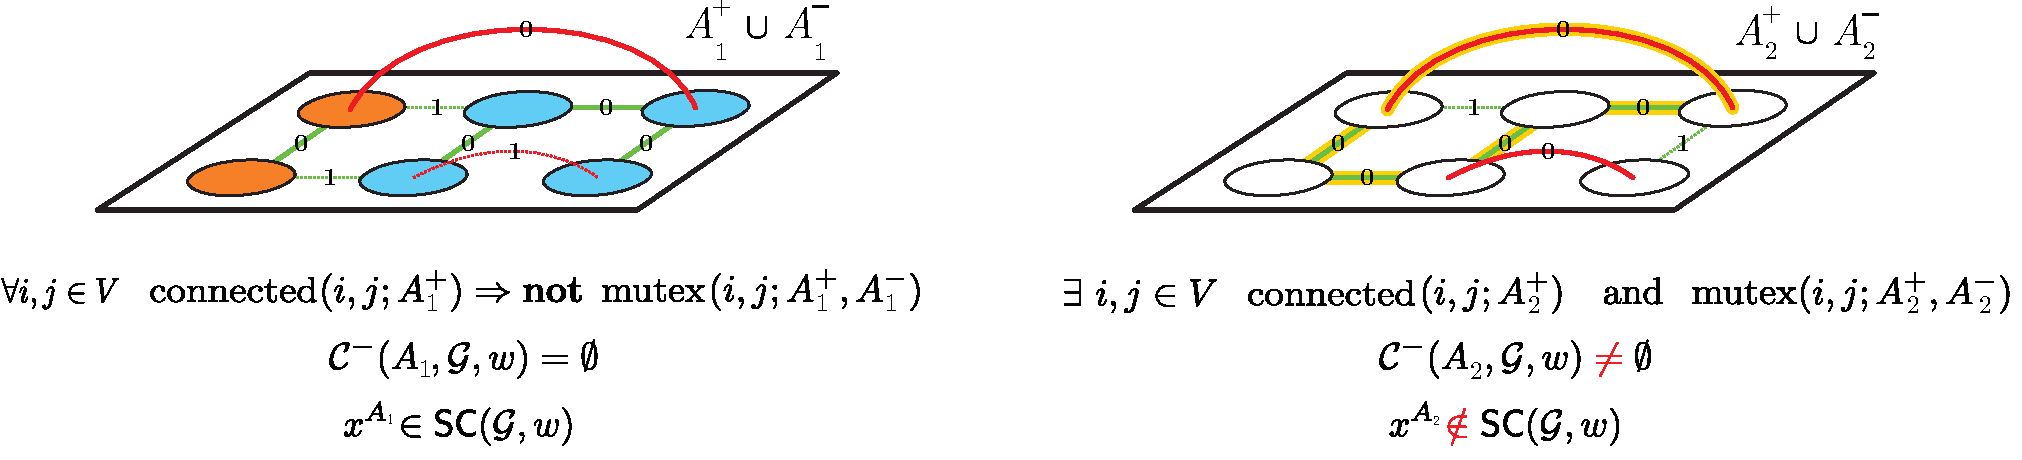
\includegraphics[width=\linewidth]{figures/MWS/images/consistent-sets-combined.pdf}
    % \begin{subfigure}[t]{0.45\textwidth}
    %     \centering
    %     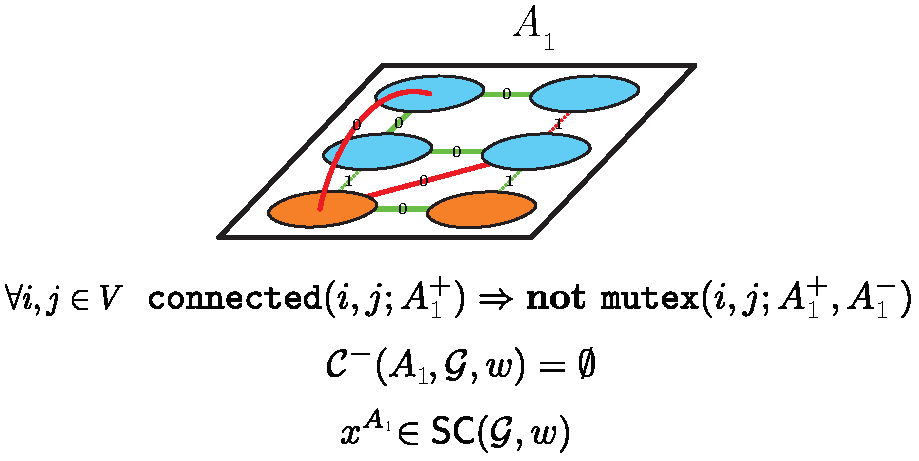
\includegraphics[width=\linewidth]{images/consistent-sets.pdf}
    %     % \caption{Consistent active sets}
    %     % $\mathcal{C}^-(A, \mathcal{G},w)=\emptyset \quad x^A\in \mathsf{SC}(\mathcal{G}, w)\quad \operator{connected}(i, j; A^+) \Rightarrow \textbf{not } \operator{mutex}(i, j; A^+,A^-)$.
    % \end{subfigure}%
    % \hfill 
    % \begin{subfigure}[t]{0.45\textwidth}
    %     \centering
    %     \includegraphics[width=\linewidth]{images/inconsistent-sets.pdf}
    %     % \caption{$\mathcal{C}^-(A, \mathcal{G},w)\neq \emptyset \quad x^A\notin \mathsf{SC}(\mathcal{G}, w)\quad \operator{connected}(i, j; A^+) \nRightarrow \textbf{not } \operator{mutex}(i, j; A^+,A^-)$}
    % \end{subfigure} \hfill 
    \caption{\textbf{Consistent and inconsistent active sets} -- Two different active edge sets $A_1\subseteq E$ (on the left) and $A_2\subseteq E$ (on the right) on identical toy graphs with six nodes, attractive~(green) and repulsive~(red) edges. The value of the edge indicator $x^A\in \{0,1\}^{|E|}$ defined in Eq.~\ref{def:active_edge_indicator} is shown for every edge. Members of the active sets are shown as solid lines.  \textbf{On the left}, the active set $A_1$ is \emph{consistent}, i.e. does not include any conflicted cycle $\mathcal{C}^-(\mathcal{G},w)$ (see Def. \ref{def:conflicted_cycles}): Therefore, it is associated with a clustering (represented by arbitrary node colors). \textbf{On the right}, the active set $A_2$ is not consistent and includes at least one conflicted cycle (highlighted in yellow), thus it cannot be associated with a node clustering.}
\label{fig:conflicted_cycles}
\end{figure*}


\section{Theoretical characterization}\label{sec:MWS_objective}

\noindent \textbf{Towards the Multicut framework.}
In section \ref{3_3_MWS}, we have introduced the Mutex Watershed (MWS) algorithm as a generalization of seeded watersheds and the Kruskal algorithm in particular. 
However, since we are considering graphs with negative edge weights, the MWS is conceptually closer to the multicut problem and related heuristics such as GAEC and GF \cite{levinkov2017comparative}.
Fortunately, due to the structure of the MWS it can be analyzed using dynamic programming. This section summarizes our second contribution, i.e. the proof that the Mutex Watershed Algorithm globally optimizes a precise objective related to the multicut.

\subsection{Review of the Multicut problem and its objective}
In the following, we will review the multicut problem not in its standard formulation but in the \textit{Cycle Covering Formulation} introduced in \cite{lange2018partial}, which is similar to the MWS formulation as it also considers the set of \textit{attractive} and \textit{repulsive} edges separately. 
Previously, in Sec.~\ref{sec:notation}, we defined a clustering by introducing the concept of an active set of edges \mbox{$A=A^+\cup A^-\subseteq E$} and the \operator{connected/}\operator{mutex} predicates. In particular, an active set describes a valid clustering if it does not include \textbf{both} a path of only attractive edges \textbf{and} a path with exactly one repulsive edge connecting any two nodes $i,j\in V$:
\begin{equation}
\operator{connected}(i, j; A^+) \quad \Longrightarrow \quad \textbf{not } \operator{mutex}(i, j; A^+,A^-).
\end{equation}
In other words, an active set is \emph{consistent} and describes a clustering if it does not contain any cycle with exactly one repulsive edge (known as conflicted cycles). 

\begin{definition} \label{def:conflicted_cycles}
\textbf{Conflicted cycles} --
We call a cycle of $\mathcal{G}$ conflicted w.r.t. $(\mathcal{G},w)$ if it contains precisely one repulsive edge $e \in E^-$, s.t. $w_e < 0$. We denote by $\mathcal{C}^-(\mathcal{G},w) \subseteq \mathcal{C}(\mathcal{G},w)$ the set of all conflicted cycles. Furthermore, given a set of edges $A \subseteq E$, we denote by $\mathcal{C}^-(A, \mathcal{G},w) \subseteq \mathcal{C}^-(\mathcal{G},w)$ the set of conflicted cycles involving only edges in $A$.
\end{definition}

\noindent 
From now on, in order to describe different clustering solutions in the framework of (integer) linear programs, we associate each active set $A$ with the following edge indicator $x^A$
\begin{equation}
         x^A := \mathbbm{1}\{e \notin A)\} \in \{0,1\}^{|E|}. \label{def:active_edge_indicator}
\end{equation}
In this way, the cycle-free property $\mathcal{C}^-(A, \mathcal{G},w)=\emptyset$ of an active set can be reformulated in terms of linear inequalities:
\begin{equation}
\forall C \in \mathcal{C}^-(\mathcal{G},w): \sum_{e\in E_C} x^A_e \geq 1 \quad \Longleftrightarrow \quad \mathcal{C}^-(A, \mathcal{G},w) = \emptyset. \label{eq:cycles_and_linear_ineq}
\end{equation}
In words, the active set cannot contain conflicted cycles; or vice versa, every conflicted cycle must contain at least one edge that is not part of the active set.
Following \cite{lange2018partial}, via this property we describe the space of all possible clustering solutions by defining the convex hull $\mathsf{SC}(\mathcal{G}, w)$ of all edge indicators corresponding to valid clusterings of $(\mathcal{G}, w)$:
\begin{definition}\label{def:set_covering_hull}
Let $\mathsf{SC}(\mathcal{G}, w)$ denote the convex hull of all edge indicators \mbox{$x \in \{0,1\}^{|E|}$} satisfying the following system of inequalities:
\begin{equation} 
\forall C \in \mathcal{C}^-(\mathcal{G},w): \quad \sum_{e\in E_C} x_e \geq 1. \label{eq:def_set_covering_hull}
\end{equation} 
That is, $\mathsf{SC}(\mathcal{G}, w)$ contains all edge labelings for which every conflicted cycle is broken at least once. We call $\mathsf{SC}(\mathcal{G}, w)$ the set covering polyhedron with respect to conflicted cycles, similarly to \cite{lange2018partial}.
\end{definition}


\noindent Fig.~\ref{fig:conflicted_cycles} summarizes these definitions and provides an example of consistent and inconsistent active sets with their associated clusterings and edge indicators.  

As shown in \cite{lange2018partial}, the \emph{multicut optimization problem} can be formulated with constraints over conflicted cycles in terms of the following integer linear program (ILP), which is NP-hard:
\begin{gather}
\min_{x \in \mathsf{SC}(\mathcal{G},w)} \sum_{e\in E} |w_e| x_e.
\label{eq:MC_set_covering_problem}
\end{gather}
The solution of the multicut problem is given by the clustering associated to the connected components of the active set $\hat{A}^+=\{e\in E^+|\hat{x}_e=0\}$, where \mbox{$\hat{x} \in \{0,1\}^{|E|}$} is the solution of (\ref{eq:MC_set_covering_problem}).

\subsection{Mutex Watershed Objective}\label{sec:MWS_objective_sub}

We now define the Mutex Watershed objective that is minimized by the Mutex Watershed Algorithm~(proof in \autoref{sec:optimality_MWS}) and show how it is closely related to the multicut problem defined in Eq. (\ref{eq:MC_set_covering_problem}). 
Lange et al.\ \cite{lange2018partial} introduce the concept of dominant edges in a graph. For example, an attractive edge $f \in E^+$ is called dominant if 
there exists a cut $B$ with $f \in E_B$ such that 
$|w_{f}| \geq \sum_{e \in E_{B} \backslash\{f\}}\left|w_{e}\right|$.
\REVIEW{These highlight an aspect of the multicut problem that can be used to search for optimal solutions more efficiently.}
Not all weighted graphs contain dominant edges; but if, assuming no ties, we raise all graph weights to a large enough power a similar property emerges.
\begin{definition}\label{def:pineq}
\textbf{Dominant power:}
Let $\mathcal{G} = (V, E, w)$ be an edge-weighted graph, with unique weights $w: E \rightarrow \mathbb{R}$. We call $p \in \mathbb{N}^+$ a dominant power if:
\begin{equation}
    |w_e|^p > \sum_{t \in E,\; w_t < w_e} |w_t|^p \qquad \forall e \in E, \label{eq:pcondition}
\end{equation}
\end{definition}
 \noindent In contrast to dominant edges \cite{lange2018partial}, we do not consider edges on a cut but rather all edges with smaller absolute weight. Note that there exists a dominant power for any finite set of edges, since for any $e \in E$ we can divide (\ref{eq:pcondition}) by $|w_e|^p$ and observe that the normalized weights $|w_t|^p/|w_e|^p$ (and any finite sum of these weights) converges to 0 when $p$ tends to infinity. 

 By considering the multicut problem in Eq. (\ref{eq:MC_set_covering_problem}) and raising the weights $|w_e|$ to a dominant power $p$, we fundamentally change the problem structure:
 \begin{definition}\label{def:MWS_objective}
\textbf{Mutex Watershed Objective:}
Let $\mathcal{G} = (V, E, w)$ be an edge-weighted graph, with unique weights $w:E \rightarrow \mathbb{R}$ and $p \in \mathbb{N}^+$ a dominant power. Then the Mutex Watershed Objective is defined as the integer linear program
\begin{equation}
  \min_{x \in \mathsf{SC}(\mathcal{G}, w)} \quad \sum_{e \in E}  |w_e|^p \, x_e  \label{eq:MWS_objective_SC}
\end{equation}
where $\mathsf{SC}(\mathcal{G}, w)$ is the convex hull defined in Def.~\ref{def:set_covering_hull}.
\end{definition}

In the following section, we will prove that this modified version of the multicut objective, which we call Mutex Watershed Objective, is indeed optimized by the Mutex Watershed Algorithm:

\begin{restatable}{theorem}{Objective}\label{theo:optimal_v1}
Let $\mathcal{G} = (V, E, w)$ be an edge-weighted graph, with unique weights $w:E \rightarrow \mathbb{R}$ and $p \in \mathbb{N}^+$ a dominant power. Then the edge indicator given by the Mutex Watershed Algorithm \ref{algo_code_efficient} $$x^{\mathbf{MWS}} := \mathbbm{1}\Big\{e \notin \mathbf{MWS}\Big(\mathcal{G}, w, \operator{connect\_all=True}\Big)\Big\}$$ minimizes the Mutex Watershed Objective in Eq.~(\ref{eq:MWS_objective_SC}).
\end{restatable} 
\noindent 

\subsection{Proof of optimality via dynamic programming} \label{sec:optimality_MWS}

\begin{algorithm}[t]
  \caption{Conflicted-Cycles Mutex Watershed}
  \begin{algorithmic}[1]
      \Procedure{ConflictedCyclesMWS}{$\mathcal{G}(V,E),w:E\rightarrow \mathbb{R}$}
      \State $A \leftarrow \emptyset$\;
      \For{$(i,j) = e \in E $ {\rm in descending order of } $|w_e|$}     
          \If{\rm $\mathcal{C}^-(A\cup \{e\},\mathcal{G},w) = \emptyset$}
              \State $A \leftarrow A \cup e$
          \EndIf
        \EndFor
        \State
        \Return $A$
      \EndProcedure
  \end{algorithmic}
    \label{MWS_conflicted_cycles}
\algcomment{Equivalent formulation of the Mutex Watershed Algorithm \ref{algo_code_efficient}, \REVIEW{with input parameter $\operator{connect\_all=True}$}. The set of conflicted cycles $\mathcal{C}^-(A,\mathcal{G},w)$ is defined in Def. \ref{def:conflicted_cycles}. The output clustering is defined by the connected components of the final attractive active set $A^+=A\cap E^+$.}

\end{algorithm}


% \begin{algorithm}[b]
%  \hrulefill \\
%  \textbf{Conflicted-Cycles Mutex Watershed:}\\
% \SetKwProg{CCMWS}{CCMWS}{$\big(\mathcal{G}(V,E),w:E\rightarrow \mathbb{R}\big)$:}{}
% \CCMWS{}{
%  $A \leftarrow \emptyset$\;
%  \For{$(i,j) = e \in E $ {\rm in descending order of } $|w_e|$} 
%  {
%     \If{\rm $\mathcal{C}^-(A\cup \{e\},\mathcal{G},w) = \emptyset$}{
%           $A \leftarrow A \cup e$\;
    
%     }
%  }
%  \Return $A$\;
%  }
%   \vspace{3pt}
% \hrulefill
%  \vspace{3pt}
%  \caption{Equivalent formulation of the Mutex Watershed Algorithm \ref{algo_code_efficient}, \REVIEW{with input parameter $\operator{connect\_all=True}$}. The set of conflicted cycles $\mathcal{C}^-(A,\mathcal{G},w)$ is defined in Def. \ref{def:conflicted_cycles}. The output clustering is defined by the connected components of the final attractive active set $A^+=A\cap E^+$.}
%  \label{MWS_conflicted_cycles}
% % }
% \end{algorithm}

In this section we prove Theorem \ref{theo:optimal_v1}, i.e.\ that the Mutex Watershed Objective defined in \ref{def:MWS_objective} is solved to optimality by the Mutex Watershed Algorithm \ref{MWS_conflicted_cycles}. Particularly, in the following Sec.~\ref{sec:cycle_consistency} we show that the edge indicator associated to the solution of the MWS algorithm lies in $\mathsf{SC}(\mathcal{G},w)$, whereas in Sec.~\ref{sec:optimilaty_proof} we prove that it solves Eq.~\ref{eq:MWS_objective_SC} to optimality.


% In this section we reformulate the Mutex Watershed Algorithm \ref{algo_code_efficient} \REVIEW{ in the framework of graph cuts and express the ``connected'' and ``mutex'' predicates introduced in Section~\ref{sec:notation} using ``conflicted''\cite{lange2018partial} (also known as ``erroneous''\cite{demaine2006correlation}) cycles:}

% \BIG{We show that $ x^{\mathit{MWS}} \in \mathsf{SC}(\mathcal{G}, w) $ by}
% \BIG{1) defining $\mathsf{SC}$ using $\mathcal{C}^-$}
% \BIG{rewriting \autoref{MWS_conflicted_cycles}}

% \operator{\,\,is\,consistent}

% It then follows that  we consider the integer edge indicator $x \in \{0,1\}^{|E|}$ such that each edge in the set is labeled with zero, i.e. $x =\mathds{1}\{e\notin A\}$, then we can rewrite the condition $\mathcal{C}^-(A, \mathcal{G},w)=\emptyset$ in terms of the following system of inequalities  (\ref{eq:def_set_covering_hull})
% In particular, 

\subsubsection{Cycle consistency}\label{sec:cycle_consistency}
The Mutex Watershed algorithm introduced in Sec.~\ref{3_methods} iteratively builds an active set $A = A^+ \cup A^-$ such that nodes engaged in a mutual exclusion constraint (encoded by edges in $A^-$) are never part of the same cluster. In other words, this means that the active set built by the Mutex Watershed at every iteration does never include a \emph{conflicted cycle} and is always \emph{consistent}. 
In particular, for any attractive edge $(i,j) = e^+ \in E^+$ and any consistent set $A$ that fulfills $\mathcal{C}^-(A,\mathcal{G},w) = \emptyset$:
\begin{align*}
\mathbf{not }\operator{ mutex}(i, j, A^+, A^-)\quad \Leftrightarrow &\quad \mathcal{C}^-(A\cup \{e^+\},\mathcal{G},w) = \emptyset 
\intertext{Similarly, for any repulsive edge $(s,t) = e^- \in E^-$:}
\mathbf{not} \operator{ connected}(s, t, A^+) \quad \Leftrightarrow &\quad \mathcal{C}^-(A\cup \{e^-\},\mathcal{G},w) = \emptyset
\end{align*}

\noindent Therefore, we can rewrite Algorithm~\ref{algo_code_efficient}  in the form of Algorithm~\ref{MWS_conflicted_cycles}. 
This new formulation makes it clear that 
\begin{equation}
    \mathcal{C}^-\Big(\mathbf{MWS}\big(\mathcal{G}, w, \operator{connect\_all=True}\big)\Big) = \emptyset.
\end{equation}
Thus, thanks to Eq.~\ref{eq:cycles_and_linear_ineq} and definition \ref{def:set_covering_hull}, it follows that the MWS edge indicator $x^{\mathbf{MWS}}$ defined in \ref{theo:optimal_v1} lies in  $\mathsf{SC}(\mathcal{G},w)$:
\begin{equation}
    x^{\mathbf{MWS}} \in \mathsf{SC}(\mathcal{G},w).
\end{equation}


\subsubsection{Optimality}\label{sec:optimilaty_proof}
We first note that the Mutex Watershed Objective \ref{def:MWS_objective} and Theorem~\ref{theo:optimal_v1} can easily be reformulated in terms of active sets to minimize 
\begin{equation}
  \argmin_{A \subseteq E} \quad - \sum_{e \in A}  |w_e|^p  \qquad \operator{s.t.} \quad \mathcal{C}^-(A,\mathcal{G},w)=\emptyset.  \label{eq:full_problem_active_set}
\end{equation}
% \TODO{I think this is }
% \begin{restatable}{theorem}{Objective_v2}\label{theo:optimal_v2}
% Let $\mathcal{G} = (V, E, w)$ be an edge-weighted graph, with unique weights $w:E \rightarrow \mathbb{R}$ and $p \in \mathbb{N}^+$ a dominant power. Then the final active set $A^*$ of the Mutex Watershed Algorithm \ref{MWS_conflicted_cycles} is given by the following minimization problem:
% \begin{equation}
%   \argmin_{A \subseteq E} \quad - \sum_{e \in A}  |w_e|^p  \qquad \operator{s.t.} \quad \mathcal{C}^-(A,\mathcal{G},w)=\emptyset.  \label{eq:full_problem_active_set}
% \end{equation}
% This theorem is equivalent to Theorem~\ref{theo:optimal_v1} thanks to Property~\ref{set_of_all_consistent_sets}. 
% \end{restatable} 




\noindent We now generalize the Mutex Watershed (see Algorithm~\ref{algo_subproblems}) and the objective such that an initial consistent set of active edges $\Ainit \subseteq E$ is supplied:

\begin{definition} \label{def:general_MWS_obj}
\textbf{Energy optimization subproblem.}
% Given a graph $G = (V, E^+ \cup E^-)$, let us consider the set ${\sigma := \langle e_1,e_2,\ldots,e_M \rangle}$ of edges in $E$ sorted in descending order by their weight $W^+ \cup W^-$. The integer index $j_{e} \in \mathbb{N}$ denotes the sorting index of the edge $e$, so that $\sigma_{j_{e}}=e$. 
Let \mbox{$\mathcal{G} = (V, E, w)$} be an edge-weighted graph. Define the optimal solution of the subproblem as
\begin{gather} \label{eq:general_MWS_obj}
  \subproblem(\mathcal{G},\Ainit) := \underset{A \subseteq (E \setminus \Ainit)}{\text{argmin}} \; T(A) \qquad \operator{with} \quad T(A) := - \sum_{e \in A} |w_e|^p, \\
  \operator{s.t.} \quad \mathcal{C}^{-}(A \cup \Ainit, \mathcal{G}, w) = \emptyset, \label{eq:def_energy}
\end{gather}
 where $\Ainit \subseteq E$ is a set of initially activated edges such that $\mathcal{C}^{-}(\Ainit, \mathcal{G}, w) = \emptyset$. 
\end{definition}
\noindent We note that for $\Ainit = \emptyset$, the optimal solution $\subproblem(\mathcal{G},\emptyset)$ is equivalent to the solution minimizing the Mutex Watershed Objective and Eq. (\ref{eq:full_problem_active_set}).

\begin{algorithm}[t]
  \caption{Initialized Mutex Watershed}
  \begin{algorithmic}[1]
      \Procedure{InitializedMWS}{$(\mathcal{G}(V,E), w:E\rightarrow \mathbb{R}$, {\color{blue}\rm initial active set $\Ainit $}}
        \State $A \leftarrow \emptyset$
        \For{$ {\color{blue}e \in E \setminus \Ainit} $ {\rm in descending order of weight}} 
          \If{\rm $\mathcal{C}^{-}({\color{blue}A\cup \Ainit \cup \{e\}}, \mathcal{G}, w) = \emptyset$}
              \State $A \leftarrow A \cup e$
          \EndIf
        \EndFor
        \State
        \Return $A$
        \EndProcedure
  \end{algorithmic}
    \label{algo_subproblems}
\algcomment{Mutex Watershed algorithm starting from initial active set $\Ainit$. An initial set $\Ainit$ of active edges is given as additional input and the final active set is such that $A \subseteq E \setminus \Ainit$. Note that Algorithm \ref{MWS_conflicted_cycles} is a special case of this algorithm when $\Ainit= \emptyset$. Differences with Algorithm \ref{MWS_conflicted_cycles} are highlighted in blue.}
\end{algorithm}

% \begin{algorithm}[t]
% % \parbox[t]{.7\linewidth}{
%  \hrulefill \\
%   \textbf{Initialized Mutex Watershed:}\\
%   \SetKwProg{IMWS}{IMWS}{$\big(\mathcal{G}(V,E), w:E\rightarrow \mathbb{R}$, {\color{blue}\rm initial active set $\Ainit $}$\big)$:}{}
%   \IMWS{}{
%     % \TODO{add $\mathcal{C}^{-}(\Ainit, \mathcal{G}, w) = \emptyset $ ?}\;
%      $A \leftarrow \emptyset$\;
%  \For{$ {\color{blue}e \in E \setminus \Ainit} $ {\rm in descending order of weight}} 
%  {
%     \If{\rm $\mathcal{C}^{-}({\color{blue}A\cup \Ainit \cup \{e\}}, \mathcal{G}, w) = \emptyset$}{
%           $A \leftarrow A \cup e$\;
    
%     }
%  }
%  \Return $A$\;
%  }
%   \vspace{3pt}
% \hrulefill
%  \vspace{3pt}
%  \caption{Mutex Watershed algorithm starting from initial active set $\Ainit$. An initial set $\Ainit$ of active edges is given as additional input and the final active set is such that $A \subseteq E \setminus \Ainit$. Note that Algorithm \ref{MWS_conflicted_cycles} is a special case of this algorithm when $\Ainit= \emptyset$. Differences with Algorithm \ref{MWS_conflicted_cycles} are highlighted in blue.}
%  \label{algo_subproblems}
% % }
% \end{algorithm}

\begin{definition}
\textbf{Incomplete, consistent initial set:}\label{def:initialset}
For an edge-weighted graph $\mathcal{G} = (V, E, w)$  a set of edges $\Ainit \subseteq E$ is consistent if
\begin{equation}
    \mathcal{C}^{-}(\Ainit, \mathcal{G}, w) = \emptyset.
\end{equation}
$\Ainit$ is incomplete if it is not the final solution and there exists a consistent edge $\tilde{e}$ that can be added to $\Ainit$ without violating the constraints.
    \begin{equation}
 \exists\, \tilde{e} \in E \setminus \Ainit \quad \operator{s.t.} \quad  \mathcal{C}^{-}(\Ainit \cup \{\tilde{e}\}, \mathcal{G}, w) = \emptyset
\end{equation}
\end{definition}

\begin{definition}
\textbf{First greedy step:}\label{def:greedy_step}
Let us consider an incomplete, consistent initial active set $\Ainit \subseteq E$ on $\mathcal{G} = (V, E, w)$. We define 
\begin{equation}\label{eq:greedy_step}
       g := \underset{e \in (E \setminus \Ainit)}{\text{argmax}} \;  \; |w(e)| \quad \operator{ s.t. } \quad \mathcal{C}^{-}(\Ainit \cup \{e\}, \mathcal{G}, w)  =  \emptyset. 
\end{equation}
as the feasible edge with the highest weight, which is always the first greedy step of Algorithm \ref{algo_subproblems}.
% We call this the first greedy choice of the algorithm. \TODO{Comment about existence}
\end{definition}
\noindent In the following two lemmas, %we prove that if we combine the first greedy choice of the algorithm with an optimal solution of the remaining subproblem, then we always find an optimal solution of the global problem. In other words,
 we prove that the Mutex Watershed problem has an \emph{optimal substructure property} and a \emph{greedy choice property} \cite{cormen2009introduction},
% These two properties are then sufficient to prove that the greedy \autoref{algo_subproblems} optimally solves the optimization problem \ref{eq:general_MWS_obj} and that the Mutex Watershed objective defined in \autoref{eq:full_problem} is solved by the Mutex Watershed algorithm. 
which are sufficient to prove that the Mutex Watershed algorithm finds the optimum of the Mutex Watershed Objective.

% The following two theorems prove the two named properties.
% We note that when $\Ainit = \emptyset$, $\subproblem(\mathcal{G},\Ainit=\emptyset)$ is the solution of the Mutex Watershed objective defined in \autoref{eq:full_problem} and that \autoref{algo_subproblems} is equivalent to the Mutex Watershed \autoref{algo_code}.

% {\color{red}We note that in the special case the Mutex Watershed objective defined in ? is a special case of the optimization problem \ref{eq:general_MWS_obj} when $\Ainit=\emptyset$, i.e. $\subproblem(G,\emptyset)=A^*$. Similarly, \autoref{algo_code} is a special case of \autoref{algo_subproblems} when $\Ainit=\emptyset$.}


% \subsubsection{Greedy-choice property}
% We will now prove the greedy-choice property of the problem, i.e. show that by making locally optimal greedy choices, we can arrive to the globally optimal solution  
\begin{lemma} \label{theo:greedy_choice}
\textbf{Greedy-choice property.}
For an incomplete, consistent initial active set $\Ainit$ of the Mutex Watershed, the first greedy step $g$ is always part of the optimal solution $$ g \in \subproblem(\mathcal{G},\Ainit).$$% defined in Equation \ref{eq:general_MWS_obj}.
\end{lemma}
\begin{proof}
% We will prove the GCP for any arbitrary subproblem, including $A = \emptyset$. Let $A \subseteq E$ be arbitrary, fixed and cycle free ${C}_{0/1}(A) = \emptyset$. The fist edge added by the Mutex Watershed Algorithm is 
% the consistent edge with the highest weight\footnote{We assume here that the subproblem defined by $A$ is non-trivial, such that there are consistent edges to select and $g$ is well-defined}.\\

\noindent We will prove the theorem by contradiction by assuming that the first greedy choice is not part of the optimal solution, i.e. $g \notin \subproblem(\mathcal{G},\Ainit)$. 
% \noindent Assume $ S^*(A)$ is the optimal solution of (\ref{eq:sub_problem}) that does not contain $g \notin  S^*(A)$.
Since $g$ is by definition the feasible edge with highest weight, it follows that:
\begin{equation}
|w(e)| < |w(g)| \quad \forall e \in \subproblem(\mathcal{G},\Ainit).%, \quad \mathcal{C}_{0/1}(\Ainit \cup \{e\}) = \emptyset.
\end{equation}
\noindent We now consider the alternative active set $A' = \{g\}$, that is a consistent solution, with 
\begin{equation}
T(A') = -|w_g|^p \overset{(\ref{eq:pcondition})}{<} -\sum_{t \in \subproblem(\mathcal{G},\Ainit)} |w_t|^p = T\Big(\subproblem(\mathcal{G},\Ainit)\Big)
\end{equation}
which contradicts the optimality of $\subproblem(\mathcal{G},\Ainit)$.
\end{proof}



\begin{lemma}\label{theo:optm_sub_prop}
\textbf{Optimal substructure property.}
% \TODO{Feasible problem}
Let us consider an initial active set $\Ainit$, the optimization problem defined in Equation \ref{eq:general_MWS_obj}, and assume to have an incomplete, consistent problem (see Def. \ref{def:initialset}). Then it follows that:
\begin{enumerate}
\item After making the first greedy choice $g$, we are left with a subproblem that can be seen as a new optimization problem of the same structure;
\item The optimal solution $\subproblem(\mathcal{G},\Ainit)$ is always given by the combination of the first greedy choice and the optimal solution of the remaining subproblem.
\end{enumerate}
 
 % The optimization problem defined in \autoref{eq:general_MWS_obj} fulfills the optimal substructure property. In other words, given a problem and some of its subproblems, the optimal solutions of the subproblems are always included in the optimal solution of the initial problem. \TODO{but this is not what we are proving...}
\end{lemma}

\begin{proof}
After making the first greedy choice and selecting the first feasible edge $g$ defined in Equation \ref{eq:greedy_step}, we are clearly left with a new optimization problem of the same structure that has the following optimal solution: $\subproblem(\mathcal{G},\Ainit \cup \{g\})$. \\
In order to prove the second point of the theorem, we now show that:
\begin{equation}\label{eq:optimal_sub}
\subproblem(\mathcal{G},\Ainit) = \{g\} \; \cup \subproblem(\mathcal{G},\Ainit \cup \{g\}).
\end{equation}
% Using (\ref{eq:sub_problem_with_g}) and (\ref{eq:sub_problem_without_g}) we can divide the optimization into two subproblems and choose the solution with higher energy:
% \begin{align}
%     S^*(A) = \underset{S \in \{S^{*}_{\text{+g}}(A), S^{*}_{\text{-g}}(A)\}}{\text{argmax}} T(S)
% \end{align}
Since algorithm \ref{algo_subproblems} fulfills the greedy-choice property, ${g\in \subproblem(\mathcal{G},\Ainit)}$ and we can add the edge $g$ as an additional constraint to the optimal solution:
\begin{align}
\begin{split}
  \subproblem(\mathcal{G},\Ainit) = & \underset{A \subseteq (E \setminus \Ainit)}{\text{argmin}} \quad T(A) \\
  \text{s. t.}& \quad \mathcal{C}^{-}(A \cup \Ainit, \mathcal{G}, w) = \emptyset; \quad g \in A \label{eq:optimal subproblem}
\end{split}
% \end{align}
\intertext{Then it follows that:}
% \begin{align}
\begin{split}
  \subproblem(\mathcal{G},\Ainit) = &\; \{g\} \; \cup \underset{A \subseteq \; E \setminus (\Ainit \cup \{g\})}{\text{argmin}} \quad T(A) \\
  \text{s. t.}& \quad  \mathcal{C}^{-}\Big(A \cup \{g\} \cup \Ainit, \mathcal{G}, w \Big) = \emptyset
\end{split}
\end{align}
which is equivalent to Equation \ref{eq:optimal_sub}.
% \begin{equation} \Longleftrightarrow \qquad
%   \subproblem(\mathcal{G},\Ainit) = \{g\} \; + \subproblem(\mathcal{G},\Ainit \cup \{g\})
% \end{equation}
% Therefore $\subproblem' = S^{*}(A \cup \{g\})$
% is optimally solved within $S^{*}(A$).
\end{proof}
% Finally, using Theorem \ref{theo:greedy_choice} and Theorem \ref{theo:optm_sub_prop}, we are then able to prove that the Mutex Watershed Objective defined in Equation \ref{eq:full_problem} is optimally solved by the Mutex Watershed algorithm \ref{algo_code}.
% \Objective*
\begin{proof}[\textbf{Proof of Theorems \ref{theo:optimal_v1}}]% and \ref{theo:optimal_v2}}]
In Lemmas \ref{theo:greedy_choice} and \ref{theo:optm_sub_prop} we have proven that the optimization problem defined in \ref{eq:full_problem_active_set} has the optimal substructure and a greedy choice property. 
% These two properties are then sufficient to prove that the greedy \autoref{algo_subproblems} optimally solves the optimization problem \ref{eq:general_MWS_obj} and that the Mutex Watershed objective defined in \autoref{eq:full_problem_active_set} is solved by the Mutex Watershed algorithm. 
It follows through induction that the final active set $\mathbf{MWS}\big(\mathcal{G}, w, \operator{connect\_all=True}\big)$ found by the Mutex Watershed Algorithm \ref{MWS_conflicted_cycles} is the optimal solution for the Mutex Watershed objective (\ref{eq:full_problem_active_set}) \cite{cormen2009introduction}.
\end{proof}




\subsection{Relation to the extended Power Watershed framework}\label{sec:power_ws}
The Power Watershed \cite{powerws} is an important framework for graph-based image segmentation that includes several algorithms like seeded watershed, random walker and graph cuts. Recently, \cite{najman2017extending} extended the framework to even more general types of hierarchical optimization algorithms thanks to the use of $\Gamma$-theory and \mbox{$\Gamma$-convergence} \cite{dal2012introduction,braides2006handbook}.
In this section, we show how the Mutex Watershed algorithm can also be included in this extended framework\footnote{The connection between the Mutex Watershed and the extended Power Watershed framework was kindly pointed out by an anonymous reviewer.} and how the framework suggests an optimization problem that is solved by the Mutex Watershed.

\subsubsection{Mutex Watershed as hierarchical optimization algorithm}
We first start by introducing the extended Power Watershed framework and restating the main theorem from \cite{najman2017extending}: 
\begin{theorem} \label{theorem:PW_framework}
\textbf{\cite{najman2017extending} Extended Power Watershed Framework.}
Consider three strictly positive integers $p,m,t\in \mathbb{N}^+$ and $t$ real numbers 
\begin{equation}
    1 \geq \lambda_0 > \lambda_1 > \ldots \lambda_{t-1}>0 \label{eq:sorted lambda}
\end{equation}
Given $t$ continuous functions $Q_k: \mathbb{R}^m \rightarrow \mathbb{R}$ with $0\leq k < t$, define the function
\begin{align}
Q^p(x) := \sum_{0\leq k< t} \lambda^p_k Q_k (x). \label{eq:def_Q_p}
\end{align}
% and the minimizer $x^*\in \mathbb{R}^m$ such that:
% \begin{align}
% x^* \in \lim_{p\rightarrow \infty} \argmin_{x\in \mathbb{R}^m} \, Q^p(x). \label{eq:minimizer}
% % \operator{where}\,\, Q^p(x) = \sum_{0<i\leq k} \lambda^p_i Q_i (x). 
% \end{align}
Then, if any sequence $(x_p)_{p>0}$ of minimizers $x_p$ of $Q^p(x)$ is bounded (i.e. there exists $C>0$ such that for all $p>0$, $||x_p||_{\infty}\leq C$), the sequence is convergent, up to taking a subsequence, toward a point of $M_{t-1}$, which is the set of minimizers recursively defined in Algorithm \ref{PWS_general_alg}.
% In other words, under these assumptions the minimizer $x^*$ can be found by applying the iterative/hierarchical Algorithm \ref{PWS_general_alg}.
\end{theorem}
\begin{proof}
See \cite{najman2017extending} (Theorem 3.3).
\end{proof}


\begin{algorithm}[t]
  \caption{Generic hierarchical optimization}
  \begin{algorithmic}[1]
      \Procedure{GHO}{$Q_0, \hdots, Q_{t-1}$}
           \State $M_0 = \argmin_{x \in \mathbb{R}^m} Q_0(x)$
           \For{$k \in 1, \ldots,t-1 $} 
              \State $M_k = \argmin_{x \in M_{k-1}} Q_k(x)$
            \EndFor
           % $A^* \leftarrow A$\;
           \textbf{Return: } some $x^* \in M_{t-1}$
      \State
      \Return some $x^* \in M_{t-1}$
        \EndProcedure
  \end{algorithmic}
    \label{PWS_general_alg}
\algcomment{Generic hierarchical optimization algorithm introduced in \cite{najman2017extending}. The sequence of continuous functions \mbox{$Q_k: \mathbb{R}^m \rightarrow \mathbb{R}$} is sorted according to the associated scales $\lambda_k$ (Eq.~\ref{eq:sorted lambda}).}

\end{algorithm}

% \begin{algorithm}[t]
% % \parbox[t]{.7\linewidth}{
%  \hrulefill \\
%   \textbf{Generic hierarchical optimization:}\\
%   \SetKwProg{GHO}{GHO}{($Q_0, \hdots, Q_{t-1}$):}{}
%   \GHO{}{
%    % \textbf{Inputs: }
%     % \begin{itemize}
%     % \item  A set of $t$ continuous functions $(Q_k)_{0\leq k< t}: \mathbb{R}^m \rightarrow \mathbb{R}$
%     % \item Scales 
%     % \end{itemize}
%       % \textbf{Output: }
%      % $x^*$ solution to Eq. (\ref{eq:minimizer})  
%      % \vspace{10pt}
%                % \Comment{and inherit the mutex constraints of the parent clusters}

%  $M_0 = \argmin_{x \in \mathbb{R}^m} Q_0(x)$ \\
%  \For{$k \in 1, \ldots,t-1 $} 
%  {
%   $M_k = \argmin_{x \in M_{k-1}} Q_k(x)$
%           % \Comment{\parbox[t]{.65\linewidth}{ merge $i$ and $j$ and inherit the mutex \\constraints of the parent clusters}}
%           % \Comment{merge $i$ and $j$}\\
%                % \Comment{and inherit the mutex constraints of the parent clusters}
%  }
%  }
%  % $A^* \leftarrow A$\;
%  \textbf{Return: } some $x^* \in M_{t-1}$\\
%  \vspace{-6pt}\hrulefill
%  \vspace{6pt}
%  \caption{Generic hierarchical optimization algorithm introduced in \cite{najman2017extending}. The sequence of continuous functions \mbox{$Q_k: \mathbb{R}^m \rightarrow \mathbb{R}$} is sorted according to the associated scales $\lambda_k$ (Eq.~\ref{eq:sorted lambda}).}
%  \label{PWS_general_alg}
% % }
% \end{algorithm}


We now show that the Mutex Watershed algorithm can be seen as a special case of the generic hierarchical Algorithm \ref{PWS_general_alg}, for a specific choice of scales $\lambda_k$ and functions ${Q_k(x): \mathbb{R}^{m} \rightarrow \mathbb{R}}$ (see definitions (\ref{def:scales_MWS}, \ref{eq:def_Q_k_MWS}) below) . \\

\noindent \textbf{Scales $\lambda_k$:} Let $\tilde{w}_k$ be the signed edge weights $w: E \rightarrow \mathbb{R}$ ordered by decreasing absolute value $|\tilde{w}_1| > |\tilde{w}_2| > \ldots > |\tilde{w}_{t-1}|$. If two edges share the same weight, then the weight is called $\tilde{w}_k$ for both and $E_k \subseteq E$ denotes the set of all edges with weight $\tilde{w}_k$. We then define \textit{the scales} $\lambda_k$ as 
\begin{equation}
\lambda_k := 
\begin{cases}
1 & \text{if} \,\,\, k=0 \\
\left| \frac{\tilde{w}_k}{2\tilde{w}_1} \right| & \text{otherwise.}
\end{cases}\label{def:scales_MWS}
\end{equation}

\noindent The continuous functions $Q_k(x): \mathbb{R}^{|E|} \rightarrow \mathbb{R}$ are defined as follows
\begin{equation}
Q_k(x) := 
\begin{cases}
|E|\cdot \min_{x' \in \mathsf{\intSC}(\mathcal{G},w)} ||x'-x|| \quad & \text{if } k=0\\
\sum_{e\in E_k} x_e & \text{otherwise,}\\
\end{cases} \label{eq:def_Q_k_MWS}
\end{equation}
where $\mathsf{\intSC}(\mathcal{G},w)$ is defined as:
\begin{equation}
\mathsf{\intSC}(\mathcal{G},w) := \mathsf{SC}(\mathcal{G},w) \cap \{0,1\}^{|E|}. \label{def:\intSC}
\end{equation}
In words, $Q_0(x)$ is proportional to the distance between $x$ and the closest point on the set $\mathsf{\intSC}(\mathcal{G},w)$, whereas $Q_k(x)$ depends only on the indicators $x_e$ of edges in $E_k$, for $k>0$. 


Algorithm \ref{PWS_general_alg_MWS} is obtained by substituting the scales $\lambda_k$ and functions $Q_k(x)$ (respectively defined in Eq. (\ref{def:scales_MWS}) and (\ref{eq:def_Q_k_MWS})) into Algorithm \ref{PWS_general_alg} .  
The algorithm starts by setting $M_0$ to $\mathsf{\intSC}(\mathcal{G},w)$, i.e. by restricting the space of the solutions only to integer edge labelings $x$ that do not include any conflicted cycles. Then, in the following iterations $k \in 1, \ldots,t-1 $, the algorithm solves a series of minimization sub-problems that in the most general case are NP-hard, even though they involve a smaller set of edges $E_k\subseteq E$. 
Nevertheless, if we assume that all weights are distinct, then $|E_k|=1$ for all $k$ and the solution to the sub-problems amounts to checking if the new edge can be labeled with $x_e=0$ without introducing any conflicted cycles. This procedure is identical to Algorithm \ref{algo_code_efficient}: at every iteration, the Mutex Watershed tries to add an edge to the active set $A$, provided that no mutual exclusion constraints are violated. 

In summary, the framework in \cite{najman2017extending} provides a new formulation of the Mutex Watershed Algorithm that is even applicable to graphs with tied edge weights. In practice, when edge weights are estimated by a CNN, we do not expect tied edge weights.


\begin{algorithm}[t]
  \caption{PowerWatershed Mutex Watershed}
  \begin{algorithmic}[1]
    \Procedure{PWSMWS}{$Q_0, \hdots, Q_{t-1}$}
        \State $M_{0} = \argmin_{x \in \mathbb{R}^{|E|}} Q_0(x)  = \mathsf{\intSC}(\mathcal{G},w)$ % \vspace{5pt}
        \For{$k \in 1, \ldots,t-1 $} 
            \State $M_k = \argmin_{x \in M_{k-1}} \sum_{e\in E_{k}} x_e$
        \EndFor
        \State
        \Return some $x^* \in M_{t-1}$
    \EndProcedure
  \end{algorithmic}
    \label{PWS_general_alg_MWS}
\algcomment{Special case of the general hierarchical Algorithm \ref{PWS_general_alg} obtained by substituting Def.~(\ref{def:scales_MWS}) and (\ref{eq:def_Q_k_MWS}). With the additional assumption of unique signed weights $w:E\rightarrow \mathbb{R}$, this algorithm is equivalent to the Mutex Watershed Algorithm \ref{MWS_conflicted_cycles}. The sequence of functions \mbox{$Q_k: \mathbb{R}^m \rightarrow \mathbb{R}$} defined in Eq.~\ref{eq:def_Q_k_MWS} is sorted according to the associated scales $\lambda_k$ in Eq.~\ref{def:scales_MWS}. $\mathsf{\intSC}(\mathcal{G},w)$ is defined in Eq.~\ref{def:\intSC}}
\end{algorithm}

% \begin{algorithm}[t]
% % \parbox[t]{.7\linewidth}{
% \SetAlgoLined
%  \hrulefill \\
%   % \textbf{PWSMWS:}\\
%   \SetKwProg{PWSMWS}{PWSMWS}{($Q_0, \hdots, Q_{t-1}$):}{}
%   \PWSMWS{}{
%    % \textbf{Inputs: } Scales $\lambda_k$ and functions $Q_k(x)$ respectively defined in Eq. (\ref{def:scales_MWS}) and (\ref{eq:def_Q_k_MWS}).\\
%    %    \textbf{Output: }
%    %   $\bar{x}$ solution to Eq. (\ref{eq:MWS_limit_2})
%    %   \vspace{10pt}

% $M_{0} = \argmin_{x \in \mathbb{R}^{|E|}} Q_0(x)  = \mathsf{\intSC}(\mathcal{G},w)$ \vspace{5pt}\\
%  \For{$k \in 1, \ldots,t-1 $} 
%  {
%   $M_k = \argmin_{x \in M_{k-1}} \sum_{e\in E_{k}} x_e$

%   % \TODO{$Q_k(x)$ is neither defined on $\mathbb{R}^m$ nor continuous}
%           % \Comment{\parbox[t]{.65\linewidth}{ merge $i$ and $j$ and inherit the mutex \\constraints of the parent clusters}}
%           % \Comment{merge $i$ and $j$}\\
%                % \Comment{and inherit the mutex constraints of the parent clusters}
%  }
%  }\vspace{5pt}
%  % $A^* \leftarrow A$\;
%  \textbf{Return: } some $x^* \in M_{t-1}$\\
%  \vspace{-6pt}\hrulefill
%  \vspace{6pt}
%  \caption{Special case of the general hierarchical Algorithm \ref{PWS_general_alg} obtained by substituting Def.~(\ref{def:scales_MWS}) and (\ref{eq:def_Q_k_MWS}). With the additional assumption of unique signed weights $w:E\rightarrow \mathbb{R}$, this algorithm is equivalent to the Mutex Watershed Algorithm \ref{MWS_conflicted_cycles}. The sequence of functions \mbox{$Q_k: \mathbb{R}^m \rightarrow \mathbb{R}$} defined in Eq.~\ref{eq:def_Q_k_MWS} is sorted according to the associated scales $\lambda_k$ in Eq.~\ref{def:scales_MWS}. $\mathsf{\intSC}(\mathcal{G},w)$ is defined in Eq.~\ref{def:\intSC}}
%  \label{PWS_general_alg_MWS}
% % }
% \end{algorithm}

\subsubsection{Convergence of the sequence of minimizers}
In this section, we see how Theorem \ref{theorem:PW_framework} also suggests a minimization problem that is solved by the Mutex Watershed algorithm. A short summary is given in the final paragraph of the section.

\noindent First, we make sure that the conditions of Theorem \ref{theorem:PW_framework} are satisfied when we apply it to Algorithm \ref{PWS_general_alg_MWS}:
\begin{restatable}{lemma}{boundedsequence}
\label{lemma:bounded_sequence}
Let us consider the scales $\lambda_k$ and continuous functions ${Q_k(x): \mathbb{R}^{|E|} \rightarrow \mathbb{R}}$ respectively defined in Eq. (\ref{def:scales_MWS}) and (\ref{eq:def_Q_k_MWS}). For any value of $p\in \mathbb{N}^+$, let $x_p \in \mathbb{R}^{|E|}$ be a minimizer of the function $Q^p(x)$ defined in Eq. (\ref{eq:def_Q_p}). Then, the minimizer $x_p$ lies in the set $\mathsf{\intSC}(\mathcal{G},w)$. From this, it follows that any sequence of minimizers $(x_p)_{p>0}$ is bounded and the conditions of Theorem \ref{theorem:PW_framework} are satisfied.
\end{restatable}
\begin{proof}
The function $Q^p(x)$ can be explicitly written as (see Eq. \ref{eq:def_Q_p}, \ref{def:scales_MWS} and \ref{eq:def_Q_k_MWS}):
\begin{align}
Q^p(x) =& \sum_{0\leq k< t} \lambda^p_k Q_k (x) \\
= & \, |E| \min_{x' \in \mathsf{\intSC}(\mathcal{G},w)} ||x-x'|| + \sum_{1 \leq k < t} \left | \frac{\tilde{w}_k}{2\tilde{w}_1} \right |^p \sum_{e\in E_{k}} x_e  \\
 = & \, |E| \min_{x' \in \mathsf{\intSC}(\mathcal{G},w)} ||x-x'|| +  \sum_{e \in E} \left | \frac{w_e}{2\tilde{w}_1} \right |^p \,\,x_e. 
 % =: & \,\,Q_\operator{A}^p(x) + Q_\operator{B}^p(x)
\end{align}
We then denote these two terms by:
\begin{align}
Q_\operator{A}^p(x) &:= |E| \min_{x' \in \mathsf{\intSC}(\mathcal{G},w)} ||x-x'||, \\
Q_\operator{B}^p(x) &:= \sum_{e \in E} \left | \frac{w_e}{2\tilde{w}_1} \right |^p \,\,x_e. 
\end{align}

\noindent Intuitively, we now prove that the minimizer $x_p$ of $Q^p(x)$ lies in $\mathsf{\intSC}(\mathcal{G},w)$ by showing that the first term $Q_\operator{A}^p(x)$ is always ``dominant'' as compared to $Q_\operator{B}^p(x)$. \\
First, we note that the gradient of the first term $Q_\operator{A}^p(x)$ has always norm equal to $|E|$ and points in the direction of the closest point $x' \in \mathsf{\intSC}(\mathcal{G},w)$. Given a generic point $y\in \mathbb{R}^{|E|}$, the only two cases when the gradient $\nabla_x\,Q_\operator{A}^p(x)$ does not exists are: i) if $y \in \mathsf{\intSC}(\mathcal{G},w)$; ii) if there are at least two points $x'',x''' \in \mathsf{\intSC}(\mathcal{G},w)$ such that $||y-x''||=||y-x'''||$.
% \item in all other cases, the gradient points in the direction of the closest point $x' \in \mathsf{\intSC}(\mathcal{G},w)$ and has norm \mbox{$||\nabla_x\,Q_\operator{A}^p(x)||=|E|$}.
Clearly, $Q_\operator{A}^p(x)$ presents minima only in the first case, when \mbox{$y\in \mathsf{\intSC}(\mathcal{G},w)$}.\\
On the other hand, the second term $Q_\operator{B}^p(x)$ is always differentiable and the norm of its gradient is never greater than $\sqrt{|E|}$:
\begin{equation}
\left|\left|\nabla_x\,Q_\operator{B}^p(x)\right|\right| < \left|\left| \nabla_x \left(\sum_{e \in E} x_e\right) \right|\right| = \sqrt{|E|}
% \sum_{e \in E} \left | \frac{\tilde{w}_k}{2\tilde{w}_1} \right |^p \,\,x_e <
\end{equation}
where we used the fact that $\tilde{w}_k / 2\tilde{w}_1<1$ for every \mbox{$1\leq k < t$}. 
Thus, the magnitude of the gradient given by the first term is always larger compared to the one given by the second term. We then conclude that the objective can always be reduced unless $x_p$ is a point of $\mathsf{\intSC}(\mathcal{G},w)$.
\end{proof}
\noindent Then, given any $p\in \mathbb{N}^+$ and the Def.~(\ref{def:scales_MWS}, \ref{eq:def_Q_k_MWS}), we have that the minimization of the function $Q^p(x)$ defined in Eq.~(\ref{eq:def_Q_p}) is given by the following problem:
\begin{align}
\argmin_{x\in \mathbb{R}^m} \, Q^p(x) = & \argmin_{x\in \mathbb{R}^m} \, \sum_{0\leq k< t} \lambda^p_k Q_k (x) \label{eq:MWS_limit_1} \\
= & \argmin_{x\in \mathsf{\intSC}(\mathcal{G},w)} \, \sum_{1 \leq k < t} \left | \frac{\tilde{w}_k}{2\tilde{w}_1} \right |^p \sum_{e\in E_{k}} x_e  \\
 = & \argmin_{x\in \mathsf{\intSC}(\mathcal{G},w)} \frac{1}{|2\tilde{w}_1|^p} \sum_{e \in E} |w_e|^p \,\,x_e \label{eq:MWS_limit_2}
\end{align}
where we used Lemma \ref{lemma:bounded_sequence} and restricted the domain of the $\argmin$ operation to $\mathsf{\intSC}(\mathcal{G},w)$, so that $Q_0(x)=0$ for all $x\in \mathsf{\intSC}(\mathcal{G},w)$.

It follows from Lemma \ref{lemma:bounded_sequence} and Theorem \ref{theorem:PW_framework} that a sequence of minimizers $(x_p)_{p>0}$ of the problem (\ref{eq:MWS_limit_2}) converge, up to taking a subsequence, to the solution $x^*$ returned by Algorithm \ref{PWS_general_alg_MWS}. 
More specifically, we know that any minimizer $x_p$ of (\ref{eq:MWS_limit_2}) is in the discrete set $\mathsf{\intSC}(\mathcal{G},w)$. Hence, the convergent sequence of minimizers $(x_p)_{p>0}$ eventually becomes constant and there exists a $p'\in \mathbb{N}^+$ large enough such that $x_p=x^*$ for all $p\geq p'$. In other words, in the case of unique weights and $p\geq p'$ large enough, the solution $x^*$ of the Mutex Watershed Algorithm \ref{PWS_general_alg_MWS} solves the problem (\ref{eq:MWS_limit_2}), which is just a rescaled version of the Mutex Watershed Objective we introduced in Sec.~\ref{sec:MWS_objective_sub}.

 To summarize, we used the extended Power Watershed framework to show that the Mutex Watershed provides a solution to the minimization problem in Eq. (\ref{eq:MWS_limit_2}) for $p$ large enough. In particular, this problem suggested by the Power Watershed framework is the same one previously derived in Sec. \ref{sec:MWS_objective_sub} by linking the Mutex Watershed Algorithm to the multicut optimization problem.




%!TEX root = ../../main.tex

\section{Experiments} \label{4_results}

We evaluate the Mutex Watershed on the challenging task of 
neuron segmentation in electron microscopy (EM) image volumes.
This application is of key interest in connectomics, a field of 
neuro-science that strives to reconstruct neural wiring digrams spanning complete central nervous systems. The task requires segmentation of neurons from electron microscopy images of neural tissue -- a challenging endeavor, since segmentation has to be based only on boundary information (cell membranes) and some of the boundaries are not very pronounced. Besides, cells contain membrane-bound organelles, which have to be suppressed in the segmentation. Some of the neuron protrusions are very thin, but all of those need to be preserved in the segmentation to arrive at the correct connectivity graph. While a lot of progress is being made, currently only manual tracing or proof-reading yields sufficient accuracy for correct circuit reconstruction \cite{schlegel2017Learning}.

We validate the Mutex Watershed algorithm on the most popular neural segmentation challenge: ISBI2012 \cite{isbi2012challenge}. We estimate the edge weights using a CNN as described in Section \ref{4_cnn} and compare with other entries in the leaderboard as well as with other popular post-processing methods for the same network predictions in Section \ref{4_isbi}. 

%The connectomics community has set up three popular segmentation challenges: ISBI2012 \cite{Isbi}, SNEMI3D \cite{snemi} and CREMI \cite{cremi}. The SNEMI3D challenge has been solved by \cite{lee2016superhuman} and the groundtruth for the test dataset has been published in \cite{Kasthuri2015}. We validate the Mutex watershed algorithm on the remaining two challenges. For the ISBI challenge, we estimate the edge weights using a CNN as described in 4.2 and compare against several other post-processing methods applied to the same network predictions (4.3). For the CREMI challenge, we re-purpose the predictions of the CNN used for the current leading entry (UnetLMC2) and directly compare to the lifted multicut post-processing used there (4.4). 

\subsection{Estimating edge weights with a CNN} \label{4_cnn}
The common first step to EM segmentation is to predict which pixels belong to a cell membrane using a CNN. Different post-processing methods are then used to obtain a segmentation, see \autoref{2_rel_work} for an overview of such methods.
%from simple thresholding to globally optimal lifted multicut. The prediction can be done globally \cite{everyone} or on the cell by cell basis \cite{Januszewski2017}.
The CNN can either be trained to predict boundary pixels \cite{ciresan_12_deep-em-segmentation,beier2017multicut} or undirected affinities \cite{lee2017superhuman,funke2018large} which express how likely it is for a pixel to belong to a different cell than its neighbors in the 6-neighborhood. In this case, the output of the network contains three channels, corresponding to left, down and next imaging plane neighbors in 3D. The affinities do not  have to be limited to immediate neighbors -- in fact, \cite{lee2017superhuman} have shown that introduction of long-range affinities is beneficial for the final segmentation even if they are only used to train the network. Building on the work of \cite{lee2017superhuman}, we train a CNN to predict short- and long-range affinities and then use those directly as weights for the Mutex Watershed algorithm. 

We estimate the affinities / edge weights for the neighborhood structure shown in Figure \ref{fig:connectivity}. To that end, we define local attractive and long-range repulsive edges. When attractive edges are only short-range, the solution will consist of spatially connected segments that cannot comprise ``air bridges''. This holds true for both (lifted)~multicut and for Mutex Watershed. We use a different pattern for in-plane and between-plane edges due to the great anisotropy of the data set. In more detail, we pick a sparse ring of in-plane repulsive edges and additional longer-range in-plane edges which are necessary to split regions reliably (see Figure \ref{fig:2d-connection}).
We also added connections to the indirect neighbors in the lower adjacent slice to ensure correct 3D connectivity (see Figure \ref{fig:3d-connection}). In our experiments, we pick a subset of repulsive edges, by using strides of 2 in the XY-plane in order to avoid artifacts caused by occasional very thick membranes. Note that the stride is not applied to local (attractive) edges, but only to long-range (repulsive) edges. The particular pattern used was selected after inspecting the size of typical regions. The specific pattern is the only one we have tried and was {\it not} optimized over.
%This reduces artifacts in form of single pixel segments due to thick boundaries.
%It also decrease the runtime of the Mutex Watershed by reducing the total number of edges considered by Algorithm \ref{algo_code}.

In total, $C^+$ attractive and $C^-$ repulsive edges are defined for each pixel, resulting in $C^+ + C^-$ output channels in the network. 
We partition the set of attractive / repulsive edges into subsets $H^+$ and $H^-$ that contain all edges at a specific offset:
$\label{edgesets}
    E^+ = {\bigcup_{c=1}^{C^+}} H^+_{c}$ for attractive edges, with $H^{-}$ defined analogously. 
Each element of the subsets $H^+_{c}$ and $H^-_{c}$ corresponds to a specific channel predicted by the network. We further assume that weights take values in $[0,1]$.% and adopt the same conventions for attractiveness / repulsion as in section \ref{3_methods}. 

\subsubsection*{Network architecture and training}
We use the 3D U-Net \cite{ronneberger_15_u-net, cciccek20163d} architecture, as proposed in \cite{funke2018large}. %It is illustrated in Figure \ref{fig:architecture}.
Our training targets for attractive / repulsive edges $\gt{w}^\pm$ can be derived from a groundtruth label image $\gt{L}$ according to
\begin{equation}
    \gt{w}^+_{e=(i, j)} = \begin{cases}
        1 , &\text{ if } \gt{L}_i = \gt{L}_j\\
        0 , & \text{otherwise}
    \end{cases}\quad
\end{equation}
\begin{equation}
    \gt{w}^-_{e=(i, j)} = \begin{cases}
        0 , &\text{ if } \gt{L}_i = \gt{L}_j\\
        1 , & \text{otherwise}
    \end{cases}
\end{equation}
Here, $i$ and $j$ are the indices of vertices / image pixels.
Next, we define the loss terms:
\begin{equation} \label{dice_plus}
    \mathcal{J}^+_{c} = - \frac{\sum_{e \in H^+_{c}} (1 - w^+_e) (1 - \gt{w}^+_e)}{\sum_{e \in H^+_{c}} ((1 - w^+_e)^2 + (1 -\gt{w}^+_e)^2)} 
\end{equation}\label{dice_minus}
\begin{equation}
 \mathcal{J}^-_{c} = - \frac{\sum_{e \in H^-_{c}} w^-_e {\gt{w}^-_e}}{\sum_{e \in H^-_{c}} ((w^-_e)^2 + (\gt{w}^-_e)^2)}
\end{equation}
for attractive edges (i.e. channels) and repulsive edges (i.e. channels).

\begin{figure}[htp]
    \centering
    \begin{subfigure}[b]{0.8 \linewidth}
    \centering
    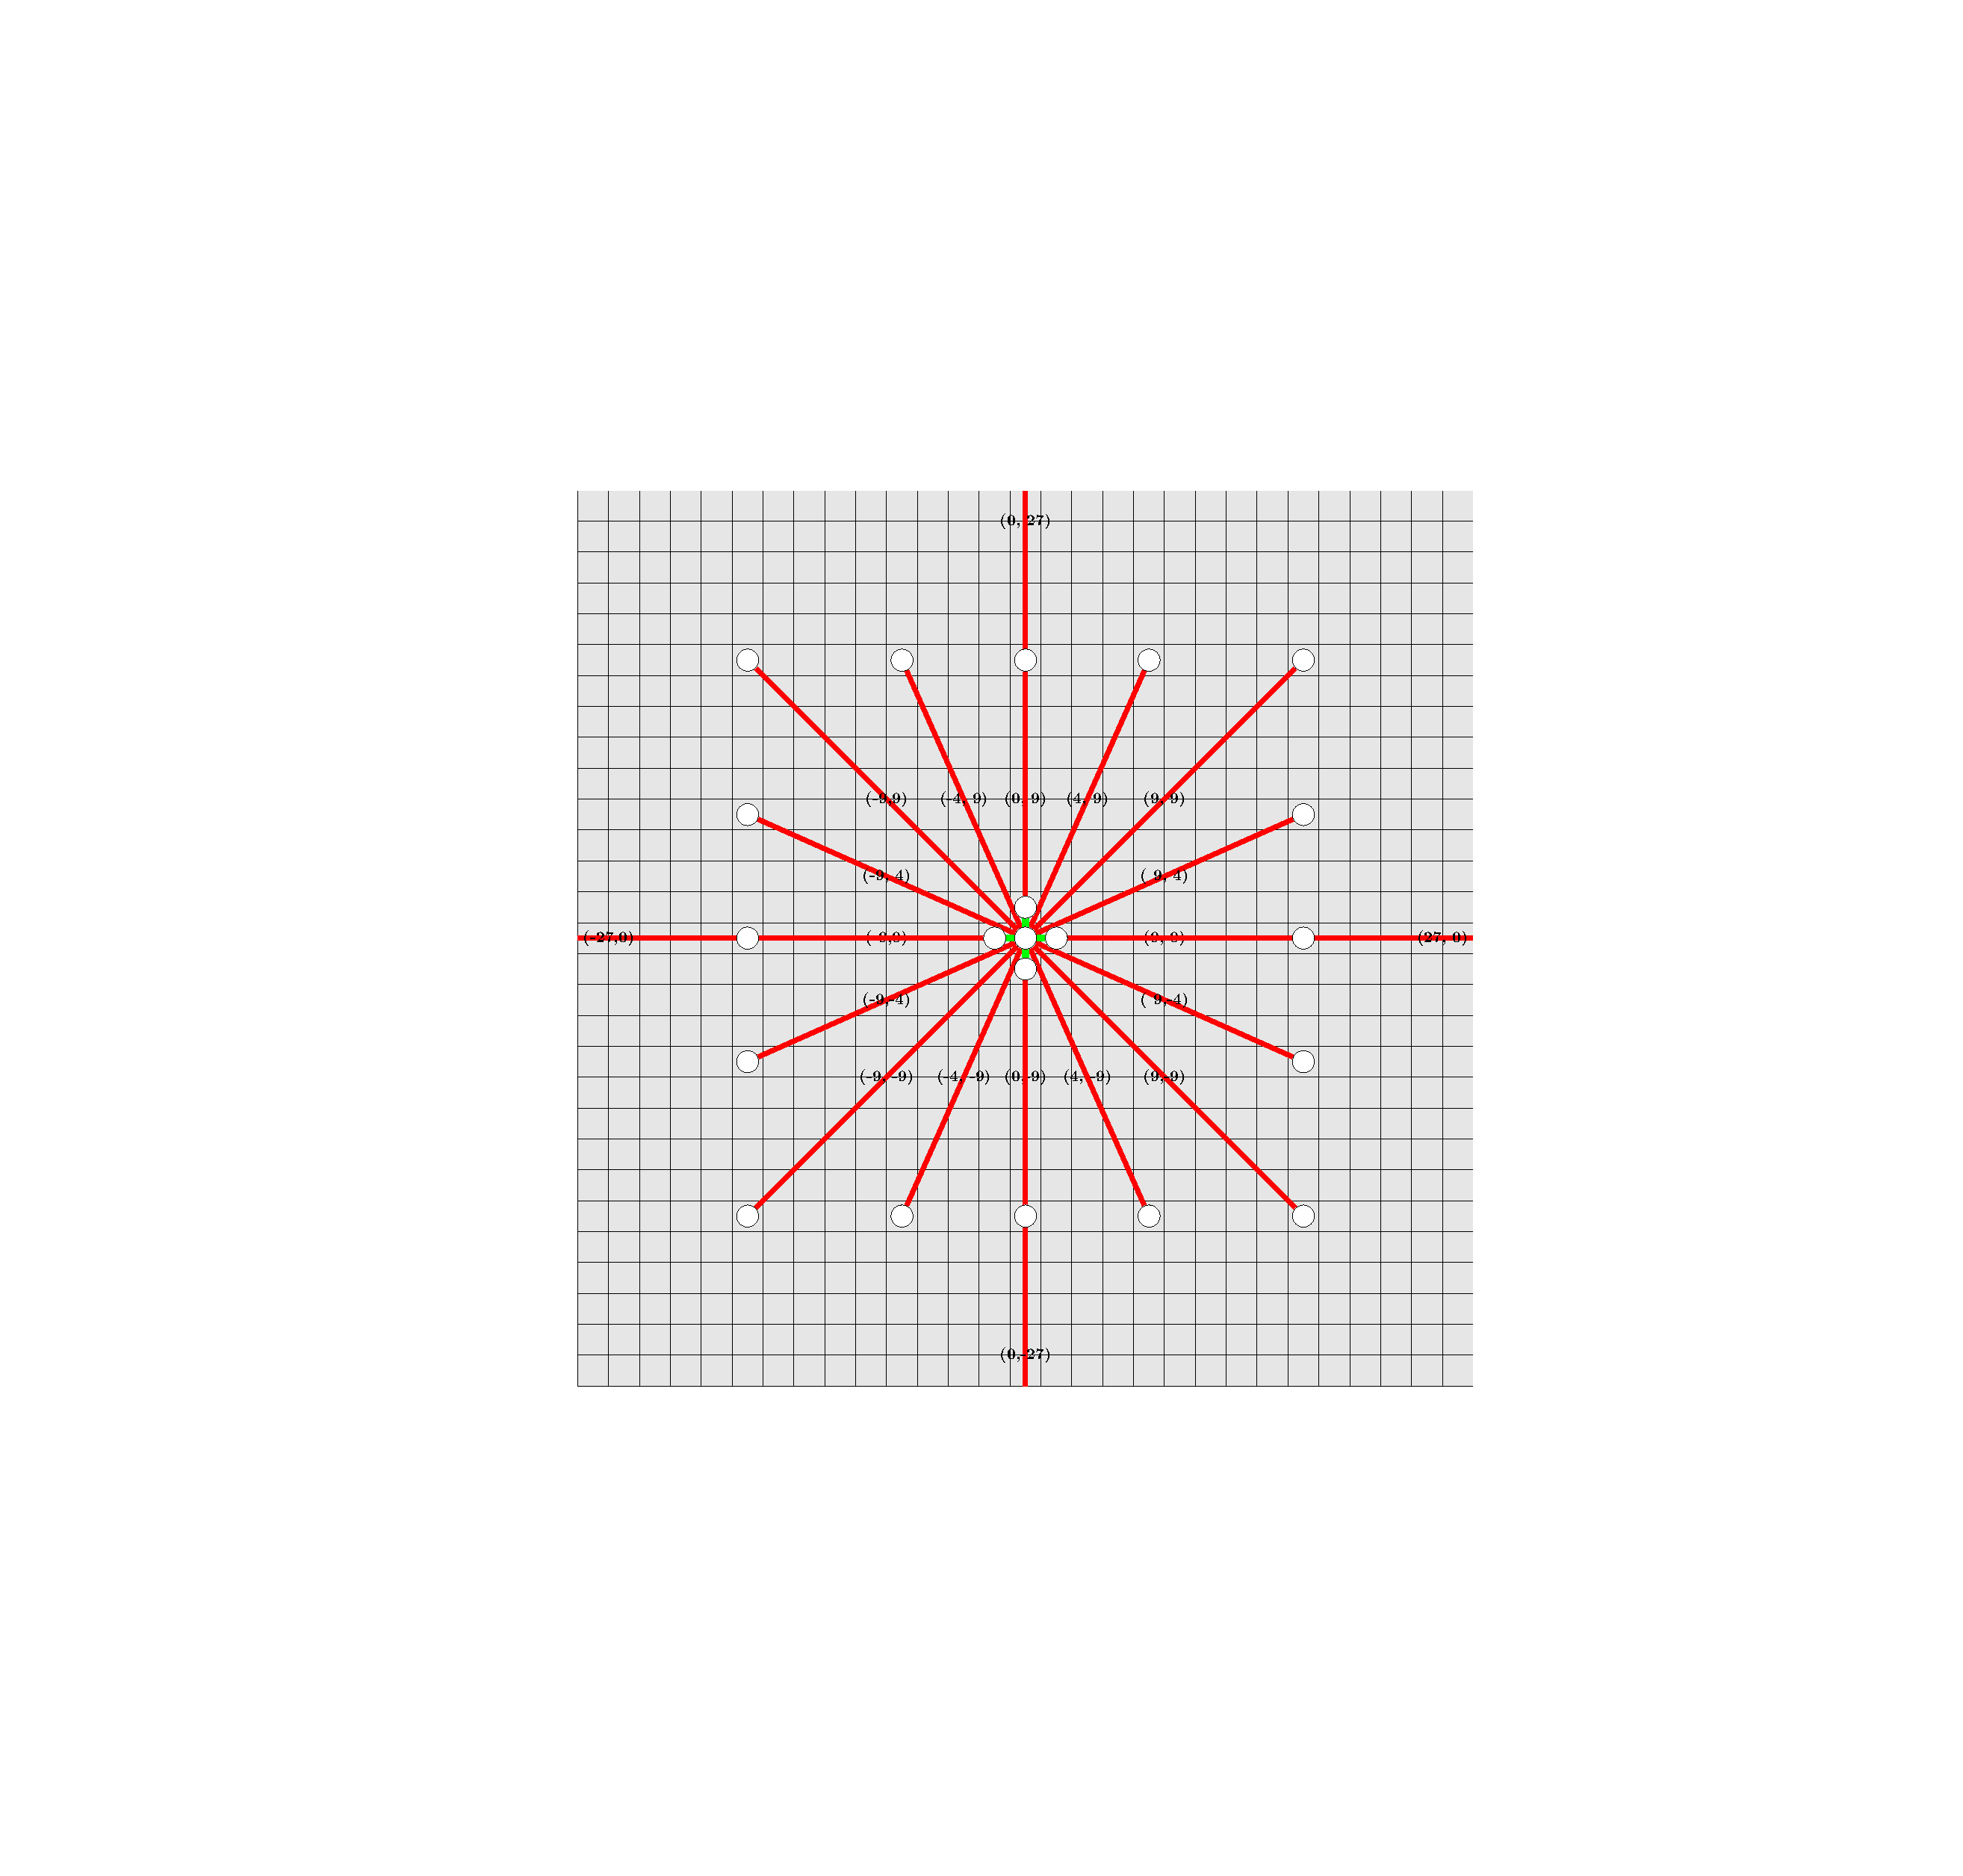
\includegraphics[width=0.9\linewidth]{figures/MWS/images/2d_connection.pdf}%
    \caption{XY-plane neighborhood with local attractive edges (green) and
     sparse repulsive edges (red) with approximate radius 9 and further long-range connections with distance 27}\label{fig:2d-connection}
    \end{subfigure}
    \par\bigskip
    \begin{subfigure}[b]{0.8 \linewidth}
    \centering
    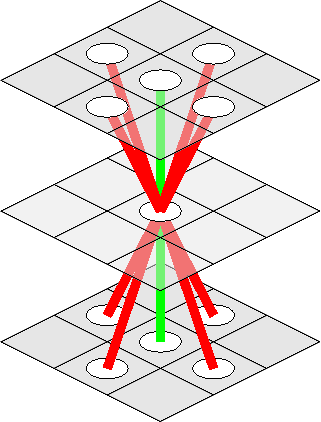
\includegraphics[width=0.4\linewidth]{figures/MWS/images/3d_connection3.pdf}
    \caption{Due to the great anisotropy of the data we limit the Z-plane edges to a distance of 1. The direct neighbors are attractive, whereas the indirect neighbors are repulsive.}\label{fig:3d-connection}
    \end{subfigure}%
    \caption{Local neighborhood structure of attractive~(green) and repulsive~(red) edges in the Mutex Watershed graph.}
    \label{fig:connectivity}
\end{figure}
Equation \ref{dice_plus} is the S{\o}rensen-Dice coefficient \cite{dice1945measures,sorensen1948method} formulated for fuzzy set membership values.
During training we minimize the sum of attractive and repulsive loss terms $\mathcal{J} = \sum_{c}^{C^+} \mathcal{J}^{+}_{c} + \sum_{c}^{C^-} \mathcal{J}^{-}_{c}$. This corresponds to summing up the channel-wise S{\o}rensen-Dice loss. 
The terms of this loss are robust against prediction and / or target sparsity, a desirable quality for neuron segmentation: since membranes are locally two-dimensional and thin, they occupy very few pixels in three-dimensional the volume. 
More precisely, if $w^{+}_e$ or $\gt{w}^{+}_e$ (or both) are sparse, we can expect the denominator $\sum_e(({w^{+}_e})^2 + (\gt{w}^+_e)^2)$ to be small,
which has the effect that the numerator is adaptively weighted higher. 
In this sense, the S{\o}rensen-Dice loss at every pixel $i$ is conditioned on the global image statistics, which is not the case for a Hamming-distance based loss like Binary Cross-Entropy or Mean Squared Error. 

We optimize this loss using the Adam optimizer \cite{kingma2014adam} and additionally condition learning rate decay on 
the Adapted Rand Score \cite{isbi2012challenge} computed on the training set every 100 iterations.
During training, we augment the data set by performing in-plane rotations by multiples of 90 degrees, flips along the X- and Y-axis as well as elastic deformations.
At prediction time, we use test time data augmentation, presenting the network with
seven different versions of the input obtained by a combination of rotations by a multiple of 90 degrees, axis-aligned flips and transpositions.
The network predictions are then inverse-transformed to correspond to the original image, and the results averaged.

\subsection{ISBI Challenge} \label{4_isbi}

The ISBI 2012 EM Segmentation Challenge \cite{isbi2012challenge} is the neuron segmentation challenge 
with the largest number of competing entries.
The challenge data contains two volumes of dimensions 1.5 $\times$ 2 $\times$ 2 microns and 
has a resolution of 50 $\times$ 4 $\times$ 4 nm per pixel. The groundtruth is provided as binary membrane
labels, which can easily be converted to a 2D, but not 3D segmentation. To train a 3D model, we follow the procedure
described in \cite{beier2017multicut}. 
\captionsetup[subfigure]{justification=centering, singlelinecheck=off}
\begin{figure}[htp]
\centering
    \begin{subfigure}[t]{0.41 \linewidth}
        \centering
        \includegraphics[width=0.98\textwidth]{figures/MWS/images/damws_2.png}
        \caption{Mutex Watershed} \label{fig:mws1}
    \end{subfigure}\hspace{0.5cm}
    \vspace{0.3cm}
    \begin{subfigure}[t]{0.41 \linewidth}
        \centering
        \includegraphics[width=0.98\textwidth]{figures/MWS/images/damws_1.png}
        \caption{Mutex Watershed} \label{fig:mws2}
    \end{subfigure}
    \vspace{0.3cm}
    \begin{subfigure}[t]{0.41 \linewidth}
        \centering
        \includegraphics[width=0.98\textwidth]{figures/MWS/images/mclr_2.png}
        \caption{Multicut partitioning based segmentation~(MC-FULL)} \label{fig:mc_full}
    \end{subfigure}\hspace{0.5cm}
    \begin{subfigure}[t]{0.41 \linewidth}
        \centering
        \includegraphics[width=0.98\textwidth]{figures/MWS/images/thresholded_1.png}
        \caption{Thresholding of local boundary maps ~(THRESH)} \label{fig:thresh}
    \end{subfigure}%
    
    \begin{subfigure}[t]{0.41 \linewidth}
        \centering
        \includegraphics[width=0.98\textwidth]{figures/MWS/images/ws_2.png}
        \caption{Watershed, seeded at local minima of the smoothed input map~(WS)} \label{fig:ws}
    \end{subfigure}\hspace{0.5cm}%
    \begin{subfigure}[t]{0.41 \linewidth}
        \centering
        \includegraphics[width=0.98\textwidth]{figures/MWS/images/wsdt_22.png}
        \caption{Distance Transform Watershed~(WSDT)} \label{fig:wsdt}
    \end{subfigure}
    % \vspace{-0.4cm}
    \caption{Mutex Watershed and baseline segmentation algorithms applied on the ISBI Challenge test data. Red arrows point out major errors. Orange arrows point to difficult, but correctly segmented regions. All methods share the same input maps.}
    \label{fig:isbi-examples}
\end{figure}% \captionsetup[figure]{justification=centering, singlelinecheck=off}
% \begin{figure}
% \centering
%     \begin{subfigure}[t]{0.45 \linewidth}
%         \centering
%         \includegraphics[width=0.91\textwidth]{images/damws_2.png}
%         \caption{Mutex Watershed} \label{fig:mws1}
%     \end{subfigure}\hspace{0.5cm}
%     \begin{subfigure}[t]{0.45 \linewidth}
%         \centering
%         \includegraphics[width=0.91\textwidth]{images/damws_1.png}
%         \caption{Mutex Watershed} \label{fig:mws2}
%     \end{subfigure}

%     \begin{subfigure}[t]{0.45 \linewidth}
%         \centering
%         \includegraphics[width=0.91\textwidth]{images/mclr_2.png}
%         \caption{Multicut partitioning based segmentation~(MC-FULL)} \label{fig:mc_full}
%     \end{subfigure}\hspace{0.5cm}
%     \begin{subfigure}[t]{0.45 \linewidth}
%         \centering
%         \includegraphics[width=0.91\textwidth]{images/thresholded_1.png}
%         \caption{Thresholding of local boundary maps ~(THRESH)} \label{fig:thresh}
%     \end{subfigure}%
    
%     \begin{subfigure}[t]{0.45 \linewidth}
%         \centering
%         \includegraphics[width=0.91\textwidth]{images/ws_2.png}
%         \caption{Watershed, seeded at local minima of the smoothed input map~(WS)} \label{fig:ws}
%     \end{subfigure}\hspace{0.5cm}%
%     \begin{subfigure}[t]{0.45 \linewidth}
%         \centering
%         \includegraphics[width=0.91\textwidth]{images/wsdt_22.png}
%         \caption{Distance Transformed Watershed~(WSDT)} \label{fig:wsdt}
%     \end{subfigure}
%     % \vspace{-0.4cm}
%     \caption{Mutex Watershed and baseline segmentation algorithms applied on the ISBI Challenge test data. Red arrows point out mayor errors. Orange arrows point to difficult, but correctly segmented regions. All methods share the same input maps.}
%     \label{fig:isbi-examples}
% \end{figure}




The test volume has private groundtruth; results can be submitted to the leaderboard.
They are evaluated based on the Adapted Rand Score (Rand-Score) and the Variation of Information Score (VI-Score) \cite{isbi2012challenge}.%, separately for each 2D plane. 
%The results are evaluated separately for the individual 2D imaging planes with final score corresponding to the average over the planes.

Our method holds the top entry in the challenge's leader board\footnote{{\href{url}{http://brainiac2.mit.edu/isbi\_challenge/leaders-board-new}}} at the time of submission, see Table \ref{tab:isbi-leaderboard}.
This is especially remarkable insofar as it is simpler than the methods holding the other 
top entries. \RED{Three out of four rely on a CNN to predict boundary locations and postprocess
its output with the complex pipeline described in \cite{beier2017multicut}.} 
This post-processing first generates superpixels via distance transform watersheds.
Then it computes a merge cost for local and long-range connections between superpixels.
Based on this, it defines a lifted multicut partioning problem that is solved approximately.
In contrast, our method finds an optimal solution of its objective purely on the pixel level.





\subsubsection*{Comparison with other segmentation methods}
The weights predicted by the CNN described above can be post-processed directly by the Mutex Watershed algorithm. To ensure a fair comparison, we transform the same CNN predictions into a segmentation using basic and state-of-the-art post-processing methods. 
We start from simple thresholding (THRESH) and seeded watershed. Since these cannot take long-range repulsions into account, we generate a boundary map by taking the maximum\footnote{The maximum is chosen to preserve boundaries.} values over the attractive edge channels. Based on this boundary map, we introduce seeds at the local minima (WS) and at the maxima of the smoothed distance transform (WSDT). For both variants, the degree of smoothing was optimized such that each region receives as few seeds as possible, without however causing severe under-segmentation. The performance of these three baseline methods in comparison to Mutex Watershed is summarized in Table~\ref{tab:isbi-baselines}. The methods were applied only in 2D, because the
high degree of anisotropy leads to inferior results when applied in 3D.
In contrast, the Mutex Watershed can be applied in 3D out of the box and yields significantly better
2D segmentation scores.


\begin{table}[t]
    \centering
    \rowcolors{2}{white}{gray!25} % \rowcolors{<starting row index>}{<dispari row color>}{<pari row color>}
        \begin{tabular}{l c c}
            \toprule
            Method                                  & \hspace{-0.5cm}Rand-Score & VI-Score \\        
            \midrule
            UNet + MWS                              & \textbf{0.98792} & \textbf{0.99183}\\        
            ResNet + LMC \cite{xiao2018deep}        & 0.98788   &  0.99072\\
            SCN + LMC \cite{weiler2017learning}     & 0.98680   &  0.99144\\
            M2FCN-MFA \cite{shen2017multi}         & 0.98383   &  0.98981\\
            FusionNet + LMC \cite{quan2016fusionnet}& 0.98365   &  0.99130\\ 
            % ICv1 + LMC \cite{beier2017multicut}     & 0.98262   &  0.98945\\        
        \end{tabular}
        \caption{Top five entries at time of submission on the ISBI 2012 EM Segmentation Challenge. Our Mutex Watershed (MWS) is state-of-the-art without relying on the complex lifted multicut postprocessing used by most other top entries.}
        \label{tab:isbi-leaderboard}
\end{table}
\begin{table}[t]
    \centering
    \rowcolors{2}{white}{gray!25} % \rowcolors{<starting row index>}{<dispari row color>}{<pari row color>}
        \begin{tabular}{l c c r}
            \toprule
            Method   & \hspace{-0.5cm}Rand-Score & VI-Score & Time [s] \\        
            \midrule
            MWS      & \textbf{0.98792} & \textbf{0.99183} & 43.3 \\        
            MC-FULL  & 0.98029   & 0.99044 & 9415.8 \\
            LMC      & 0.97990   & 0.99007 &  966.0 \\
            THRESH   & 0.91435   & 0.96961 & 0.2 \\
            WSDT     & 0.88336   & 0.96312 & 4.4 \\
            MC-LOCAL & 0.70990   & 0.86874 & 1410.7 \\
            WS       & 0.63958   & 0.89237 & 4.9 \\
            % MC-LR Repulsive  &           &         & 6834.77 \\
        \end{tabular}
        \caption{Comparison on the ISBI 2012 EM Segmentation Challenge to other segmentation strategies, all of which are based on our CNN. Runtimes were measured on a single thread of a Intel Xeon CPU E5-2650 v3 @ 2.30GHz.}
        \label{tab:isbi-baselines}
\end{table}

Qualitatively, we show patches of results in Figure \ref{fig:isbi-examples}.
The major failure case for WS (Figure \ref{fig:ws}) and WSDT (Figure \ref{fig:wsdt})
is over-segmentation caused by over-seeding a region.
The major failure case for THRESH is under-segmentation due to week boundary evidence (see Figure \ref{fig:thresh}).
In contrast, the Mutex Watershed produces a better segmentation, only causing minor over-segmentation (see Figure \ref{fig:mws1}, Figure \ref{fig:mws2}).

Note that, in contrast to most pixel-based postprocessing methods, our algorithm can take long
range predictions into account. To compare with methods which share this property, we turn to the multicut and lifted multicut-based partitioning for neuron segmentations as
introduced in \cite{andres_12_globally} and \cite{horvnakova2017analysis}. As proposed in \cite{andres2012globally}, we compute costs corresponding to edge cuts from the affinities estimated by the CNN via:
\begin{equation}
\label{mc_costs}
    s_e = \begin{cases}
        \log \frac{w^+_e}{1 - w^+_e} , &\text{ if } e \in E^+ \\
        \log \frac{1 - w^-_e}{w^-_e}, & \text{otherwise},
    \end{cases}
\end{equation}
We set up two multicut problems: the first is induced only by the short-range edges (MC-LOCAL), the other by short- and long-range edges together (MC-FULL). Note that the solution to the full connectivity problem can contain ``air bridges'', i.e. 
pixels that are connected only by long-range edges, without a path along the local edges connecting them.
However, we found this not to be a problem in practice.
In addition, we set up a lifted multicut (LMC) problem from the same edge costs.

Both problems are NP-hard, hence it is not feasible to solve them exactly on
large grid graphs. For our experiments, we use the approximate Kernighan Lin \cite{kernighan1970efficient,keuper2015efficient} solver.
Even this allows us to only solve individual 2D problems at a time.
The results for MC-LOCAL and MC-FULL can be found in Table \ref{tab:isbi-baselines}.
The MC-LOCAL approach scores poorly because it under-segments heavily.
This observation emphasizes the importance of incorporating the longer-range edges.
The MC-FULL and LMC approaches perform well. Somewhat surprisingly, the Mutex Watershed yields a better segmentation still,
despite being much cheaper in inference. We note that both MC-FULL, LMC and the Mutex Watershed are evaluated on the same long-range affinity maps (i.e. generated by the same CNN with the same set of weights). 
%\RED{Our hypothesis, to explain the superior Mutex Watershed performance over the multicut solutions, is that the MWS has no shrinking bias. This could be beneficial for certain segmentation problems with thin elongated regions.}

%  the strict separation in attractive short-range and repulsive long-range edges is beneficial for certain problems.
% This might hold true for segmentation because ``non-connectedness'' of two pixels in an image can often only be decided reliably at larger distances.




%!TEX root = ../../main.tex

\section{Conclusion and Discussion} \label{Conclusion}
We have presented a fast algorithm for the clustering of graphs with both attractive and repulsive edges. The ability to consider both
\REVIEW{gives a valid alternative to other popular graph partitioning algorithms that rely on a stopping criterion or seeds.}
 % obviates the need for the kind of stopping criterion or even seeds that all popular algorithms except for multicut / correlation clustering need. 
 The proposed method has low computational complexity in imitation of its close relative, Kruskal's algorithm. We have shown which objective this algorithm optimizes exactly, and that this objective emerges as a specific case of the multicut objective. \RED{It is possible that recent interesting work \cite{lange2018partial} on partial optimal solutions may open an avenue for an alternative proof.
%An alternative approach for our proof may be derived from the recent work by \cite{lange2018partial} on partial optimal solutions. 
% We  showing that every greedy choice can be shown to be a partial optimal solution. 
%every edge fixed the the Mutex Watershed is part of one optimal solution.%, where they show that repulsive / attractive edges are cut / not cut in the optimal multicut solution when the edge's absolute weight is larger than the sum of absolute weights of edges along a given cutntro.
}
% facilitate an alternative method to prove this property,  showing that repulsive / attractive edges are cut / not cut in the optimal multicut solution when the edge's absolute weight is larger than the sum of absolute weights of edges along a given cut.}

Finally, we have found that the proposed algorithm, when presented with informative edge costs from a good neural network, outperforms all known methods on a competitive bioimage partitioning benchmark, including methods that operate on the very same network predictions. 


% \RED{We prove using dynamic programming that -- in this limit -- the optimal partitioning can be determined iteratively in order of absolute edge weight. Recent analysis of the multicut objective \cite{lange2018partial} suggests an alternative method to prove this property,  showing that repulsive / attractive edges are cut / not cut in the optimal multicut solution when the edge's absolute weight is larger than the sum of absolute weights of edges along a given cut.}


% In future work we want to generalize our algorithm to semantic instance segmentation commonly found in natural image segmentation challenges \cite{Cordts2016Cityscapes,lin2014microsoft,mottaghi_cvpr14} and use it for end-to-end learning.

% \input{chapters/MWS/suppl_bound_sequence.tex}


%--------------------- GASP ----------------------
% !TEX root = ../../main.tex

\chapter{GASP: Generalized Agglomerative Algorithm for Signed Graph Partitioning}\label{chapter:GASP}

In this chapter, we propose a theoretical framework that generalizes simple and fast algorithms for hierarchical agglomerative clustering to weighted graphs with both attractive and repulsive interactions between the nodes. This framework defines GASP, a Generalized Algorithm for Signed graph Partitioning, and allows us to explore many combinations of different linkage criteria and cannot-link constraints. 
We prove the equivalence of existing clustering methods to some of those combinations and introduce new algorithms for combinations that have not been studied before. 
We study both theoretical and empirical properties of these combinations and prove that some of these define an ultrametric on the graph.
We conduct a systematic comparison of various instantiations of GASP on a large variety of both synthetic and existing signed clustering problems, in terms of accuracy but also efficiency and robustness to noise. 
Lastly, we show that some of the algorithms included in our framework, when combined with the predictions from a CNN model, result in a simple bottom-up instance segmentation pipeline.
Going all the way from pixels to final segments with a simple procedure, we achieve state-of-the-art accuracy on the CREMI 2016 EM segmentation benchmark without requiring domain-specific superpixels.


\begin{figure*}[t]
\centering
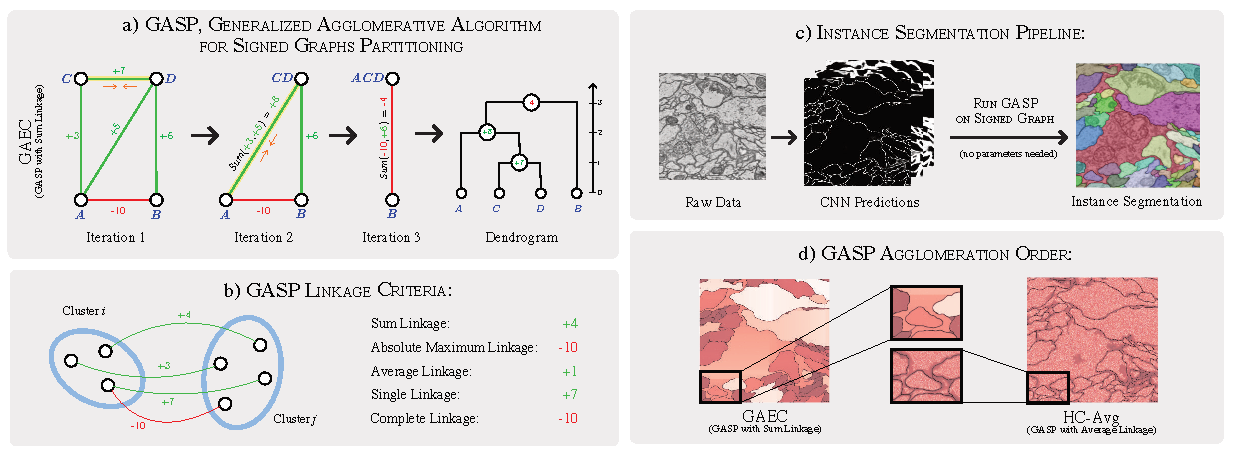
\includegraphics[width=\textwidth]{figures/GASP/intro_image_v6.pdf} % left bottom right top
\caption[GASP: some iterations on a toy graph with different linkage criteria]{\textbf{(a)} Some iterations of \algname{} on a graph with attractive (green) and repulsive (red) interactions. At each iteration, the yellow edge with highest weight is contracted (example with sum linkage criterion is shown). \textbf{(b)} Linkage criteria demonstrated on two small clusters (see definitions in Table~\ref{tab:linkage-criteria} below).  \textbf{(c)} Application of \algname{} to instance segmentation: we show raw data from the CREMI neuron-segmentation challenge and some predictions of our CNN model, where white pixels represent boundary evidence. \textbf{(d)} 
Seemingly similar linkage criteria can result in very different clustering dynamics, as shown in this example: color coded sequence of merges from early (white) via late (brown) to never (black).
% \algname{} agglomeration order for sum and average linkage: we show which pairs of neighboring pixels were merged first (white), later on (brown/red), or never (black).
\label{fig:intro_figure}}
\end{figure*}


\renewcommand\theadfont{\scriptsize}
\begin{table*}[t]
    \centering
    \scriptsize
    \begin{subtable}[t!]{\textwidth}\centering
        \begin{tabular}{c |c  c  c  c  c}
        \multicolumn{1}{c|}{\multirow{2}{*}[-1.5em]{{\Large GASP}}} 
        & \thead{Sum\\Linkage} & \thead{Absolute Maximum\\Linkage} & \thead{Average\\Linkage} & \thead{Single\\Linkage} & \thead{Complete\\Linkage} \\
 % \multicolumn{1}{c}{} 
 & $\displaystyle \sum_{e\in E_{ij}} \cost_e$  & $\displaystyle \cost_e$ with $\displaystyle e = \argmax_{t\in E_{ij}} |\cost_t|$ & $\displaystyle \sum_{e\in E_{ij}} \cost_e \bigg/ \big|E_{ij}\big| $ &  $\displaystyle \max_{e\in E_{ij}} \cost_e$ & $\displaystyle \min_{e\in E_{ij}} \cost_e$ \\ \midrule
 % \cmidrule{2-6}

            \thead[c]{Unsigned graphs} & \thead{-} &\tikzmark{a} \thead{\textbf{HC-Single}} &\tikzmark{g} \thead{\textbf{HC-Avg}} &\thead{\textbf{HC-Single}}\tikzmark{z} &\thead{\textbf{HC-Complete}} \tikzmark{b} \\
            \thead[c]{Signed graphs} & \thead{GAEC \cite{keuper2015efficient}} &  \thead{\textbf{Mutex Watershed} \cite{wolf2018mutex}}& \tikzmark{f} \thead{\textbf{HC-Avg}} &\thead{\textbf{HC-Single}} \tikzmark{e} &\thead{\textbf{HC-Complete}}\tikzmark{w} \\
            \thead[c]{Signed graphs + \\cannot-link-constr} & \thead{\colorbox{yellow}{HCC-Sum}} % \thead{Greedy Fixation \cite{levinkov2017comparative}} 
            & \thead{\textbf{Mutex Watershed} \cite{wolf2018mutex}}& \thead{\colorbox{yellow}{HCC-Avg}} &  \thead{\colorbox{yellow}{HCC-Single}} \tikzmark{d} &   \thead{\textbf{HC-Complete}} \tikzmark{c} \\
            % \multicolumn{2}{c|}{\multirow{2}{*}[-0.5em]{\thead{\textbf{\algname{} linkage criteria} $\,\,\interact(S_u ,S_v)$}}}  & \multirow{2}{*}[-0.5em]{\thead{\textbf{Unsigned Graphs}}} & \multicolumn{2}{c}{\thead{\textbf{Signed Graphs}}}  \\        
            % \multicolumn{2}{c|}{} &  &  \multicolumn{1}{c}{\thead{No Constraints}} & \thead{With Constraints} \\ \midrule
             

            %  Sum: & $\displaystyle \sum_{e\in E_{uv}} \cost_e$ & \thead{Sum Linkage\\Hier. Aggl. Clust.} & \thead{GAEC \cite{keuper2015efficient}} & \thead{Greedy\\Fixation \cite{levinkov2017comparative}} \\ 
            
             


            %  \makecell[r]{Abs. Max:} & 
            % $\displaystyle \cost_e$ with $\displaystyle e = \argmax_{t\in E_{uv}} |\cost_t|$
            %    & \thead{Single Linkage\\Hier. Aggl. Clust.} & \thead{Mutex\\Watershed \cite{wolf2018mutex}} & \thead{Mutex\\Watershed \cite{wolf2018mutex}} \\
             


            %  \makecell[r]{Average:} & $\displaystyle \sum_{e\in E_{uv}} \cost_e \bigg/ \big|E_{uv}\big|  $ & \thead{ Average Linkage\\ Hier. Aggl. Clust.} & \thead{\textbf{NEW}} & \thead{\textbf{NEW}}\\ 

            % Max: & $\displaystyle \max_{e\in E_{uv}} \cost_e$ & \thead{Single Linkage\\Hier. Aggl. Clust.} & \thead{\textbf{NEW}} & \thead{\textbf{NEW}}\\ 

            % Min:& $\displaystyle \min_{e\in E_{uv}} \cost_e$ & \thead{Complete Linkage\\ Hier. Aggl. Clust.}  & \thead{\textbf{NEW}} & \thead{\textbf{NEW}}

        \end{tabular}
    \end{subtable} 
    \caption[Conceptual contribution: Clustering algorithms in GASP framework]{Conceptual contribution: Properties of clustering algorithms included in the proposed \algname{} framework, given a linkage criterion, a type of graph (signed or unsigned) and the optional use of cannot-link constraints. New constrained hierarchical clustering algorithms (HCC) proposed in this thesis are highlighted in yellow. For algorithms typeset in bold font we prove that they define an ultrametric on the graph (Eq.~\ref{eq:UM_def}). For algorithms in the green box we show that they are weight-shift invariant (Prop.~\ref{prop:weight_shift_invariant}). 
    Notation: 
    % given a signed graph $\mathcal{G}(V,E, w_e)$, we denote as 
    $E_{ij}=(S_i \times S_{j}) \cap E$ denotes the set of edges connecting two clusters $S_i, S_j \subseteq V$. } 
    \label{tab:linkage-criteria}
\end{table*}
\renewcommand\theadfont{\normalsize}


\section{Introduction}
In computer vision, the partitioning of weighted graphs has been successfully applied to tasks as diverse as image segmentation, object tracking and pose estimation. 
Most graph clustering methods work with positive edge weights only, which can be interpreted as similarities or distances between the nodes. These methods require users to specify the desired numbers of clusters (as in spectral clustering) or a termination criterion (e.g.\ in iterated normalized cuts) or even to add a seed for each object  (e.g.\ seeded watershed or random walker).  

Other graph clustering methods work with so-called \emph{signed graphs}, which feature both positive and negative edge weights corresponding to attraction and repulsion between nodes. The advantage of signed graphs over unsigned graphs is that balancing attraction and repulsion allows us to obtain a clustering without defining additional parameters. A canonical formulation of the signed graph partitioning problem is the \emph{multicut} or \emph{correlation clustering} problem \cite{kappes2011globally,chopra1991multiway}. This problem is NP-hard, though many approximate solvers have been proposed \cite{lange2018combinatorial,pape2017solving,beier2016efficient,yarkony2012fast} together with greedy agglomerative clustering algorithms \cite{keuper2015efficient,levinkov2017comparative,wolf2018mutex,kardoostsolving}. 
Agglomerative clustering algorithms for signed graphs have clear advantages: they are parameter-free and efficient. Despite the fact that a variety of these algorithms exist, no overarching study has so far been conducted to compare their robustness and efficiency or to provide guidelines for matching an algorithm to the partitioning problem at hand. 


The first contribution presented in this chapter is a simple theoretical framework that generalizes over agglomerative algorithms for signed graphs by linking them to hierarchical clustering (HC) on unsigned graphs (Section \ref{sec:algorithm}). This framework defines an underlying basic algorithm and allows us to explore its combinations with different linkage criteria and \emph{cannot-link constraints} (see Fig.~\hyperref[fig:intro_figure]{\ref*{fig:intro_figure}a}, \hyperref[fig:intro_figure]{\ref*{fig:intro_figure}b}, and Table~\ref{tab:linkage-criteria}). 
As second contribution, in Section \ref{sec:alg_update_rules}, we formally prove that some of the combinations correspond to existing clustering algorithms, and introduce new algorithms for combinations which have not been explored before. By analyzing their theoretical properties, we also show that some of them define an ultrametric on the graph (see Table~\ref{tab:linkage-criteria}).

Third, we evaluate the algorithms on a large variety of both existing and synthetically generated signed graph clustering problems (Section \ref{sec:neuro_segm_exp}). 
Fourth and finally, we also test the algorithms on \emph{instance segmentation} -- a computer vision task consisting of assigning each pixel of an image to an object instance -- by partitioning graphs whose edge weights are estimated by a CNN (see Fig.~\hyperref[fig:intro_figure]{\ref*{fig:intro_figure}c} and Section \ref{sec:experiments_discussion}).
Our experiments show that the choice of linkage criterion markedly influences how clusters are grown by the agglomerative algorithms (Fig.~\hyperref[fig:intro_figure]{\ref*{fig:intro_figure}d}), making some linkage methods more suited for certain types of clustering problems.
% We focus our comparison on three of the best-performing algorithms included in our framework, which are based on average, sum, and absolute maximum linkage criteria (see Table~\ref{tab:linkage-criteria}). We highlight their empirical properties by showing how clusters are grown differently depending on the algorithm.
We benchmark the clustering algorithms by focusing on their efficiency, robustness and tendency to over- or under-cluster. 
On instance segmentation, we show that the tested agglomerative algorithms strongly outperform recently proposed spectral clustering methods, and that average-linkage based agglomerative algorithms achieve state of the art results on the CREMI 2016 challenge for neuron segmentation of 3D electron microscopy image volumes of brain tissue. 

\begin{tikzpicture}[remember picture,overlay]
% (shift_along_horizontal, shift_along_vertical)
% a ---------------------------- b
%            g -----------------
%            f         e ------- 
%                      d         c
% 
\draw [green,line]($(a)+(0,2ex)$)--($(b)+(0.9ex,2ex)$)--($(c)+(0.9ex,-1.5ex)$) -- ($(d)+(1.4ex,-1.5ex)$) -- ($(e)+(1.4ex,-1.2ex)$) -- ($(f)+(-0.3ex,-1.2ex)$)--($(g)+(-0.3ex,-1.2ex)$)--($(a)+(0,-1.2ex)$)--cycle;
\end{tikzpicture}

% In Sec.~\ref{sec:spectral_clust}, we also show how \algname{} outperforms spectral clustering methods on the task of neuron segmentation and how on synthetic graphs it achieves similar scores to a recently proposed spectral method for signed graphs. 
% \TODO{Define HC abbrv}

% Our code is available at \url{https://github.com/abailoni/GASP}.







% !TEX root = ../../main.tex

\section{Related work} \label{sec:related_work}
% \textbf{Proposal-based methods} have been highly successful in instance segmentation competitions like MS COCO \cite{lin2014microsoft}and CityScapes \cite{cordts2016cityscapes}. They decompose the instance segmentation task into two steps that consists in generating object proposals and assigning to each bounding box a class and a binary segmentation mask \cite{he2017mask,porzi2019seamless,liu2018path,yang2012layered,li2017fully,ladicky2010and,hariharan2014simultaneous,chen2015multi,dai2016instance,liang2016reversible}. 

\textbf{Proposal-free instance segmentation methods} adopt a bottom-up approach by directly grouping pixels into instances. In the last years, there has been a growing interest in such  methods that do not involve object detection because, in certain types of data, object instances cannot be approximated by bounding boxes \cite{kirillov2017instancecut,bai2017deep}. 
% For example, the approach proposed in \cite{kirillov2017instancecut} uses a combinatorial framework for instance segmentation, 
% SGN \cite{liu2017sgn} sequentially group pixels into lines and then instances;
% whereas a watershed transform is learned in \cite{bai2017deep} by also predicting its gradient direction. 
% whereas the template matching \cite{uhrig2016pixel} deploys scene depth information.
Some use metric learning to predict high-dimensional associative pixel embeddings that map pixels of the same instance close to each other \cite{lee2019learning,fathi2017semantic,newell2017associative,de2017semantic}
% , while mapping pixels belonging to different instances further apart \cite{lee2019learning,fathi2017semantic,newell2017associative,de2017semantic}. % kulikov2018instance
and then retrieve final instances by applying a clustering algorithm \cite{kong2018recurrentPix}.
% , like in the end-to-end trainable mean-shift pipeline of \cite{kong2018recurrentPix}. 
Other recent methods let the model predict the relative coordinates of the instance center \cite{neven2019instance,cheng2019panopticdeeplab} or, given a pixel $(x,y)$, they train a model to generate the mask of the instance located at $(x,y)$ \cite{sofiiuk2019adaptis}. 

\textbf{Edge detection} also experienced recent progress thanks to deep learning, both on natural images \cite{Gao_2019_ICCV,liu2018affinity,xie2015holistically,kokkinos2015pushing} and biological data \cite{lee2017superhuman,schmidt2018cell,meirovitch2016multi,ciresan2012deep}. In neuron segmentation for connectomics, a field of neuroscience we also address in our experiments, boundaries are converted to final instances with subsequent postprocessing and superpixel-merging:
some use a combinatorial framework \cite{beier2017multicut}, others use loopy graphs \cite{kaynig2015large,krasowski2015improving} or trees \cite{meirovitch2016multi,liu2016sshmt,liu2014modular,funke2015learning,uzunbas2016efficient} to represent the region merging hierarchy. Flood-filling networks \cite{januszewski2018high} and MaskExtend \cite{meirovitch2016multi} used a CNN to iteratively grow one region/neuron at the time.
% recently, the work of \cite{meirovitch2019cross} made the process more efficient by employing a combinatorial encoding of the segmentation.
A structured learning approach was also proposed in \cite{funke2018large,turaga2009maximin}.

\textbf{Agglomerative graph clustering} has often been applied to instance segmentation \cite{arbelaez2011contour,ren2013image,liu2016image,salembier2000binary} because of its efficiency as compared to other divisive approaches like graph cuts. 
Novel termination criteria and merging strategies have often been proposed: the agglomeration in \cite{malmberg2011generalized} deploys fixed sets of merge constraints; 
% ultrametric contour maps \cite{arbelaez2011contour} combine an oriented watershed transform with an edge detector, so that superpixels are merged until the ultrametric distance exceeds a learned threshold; 
the popular graph-based method \cite{felzenszwalb2004efficient} stops the agglomeration when the merge costs exceed a measure of quality for the current clusters. 
The optimization approach in \cite{kiran2014global} performs greedy merge decisions that minimize a certain energy, while other pipelines use classical linkage criteria, e.g.~average linkage \cite{liu2018affinity,lee2017superhuman}, median \cite{funke2018large} or a linkage learned by a random forest classifier \cite{nunez2013machine,knowles2016rhoananet}.

\textbf{Clustering of signed graphs} has the goal of partitioning a graph with both attractive and repulsive cues. Finding an optimally balanced partitioning has a long history in combinatorial optimization \cite{grotschel1989cutting,grotschel1990facets,chopra1993partition}. %and can be done without the need to specify a termination criterion. 
NP-hardness of the \emph{correlation clustering} problem was shown in \cite{bansal2004correlation}, while the connection with graph multicuts was made by \cite{demaine2006correlation}. Modern integer linear programming solvers can tackle problems of considerable size \cite{andres2012globally}, but accurate approximations \cite{pape2017solving,beier2016efficient,yarkony2012fast}, greedy agglomerative algorithms \cite{levinkov2017comparative,wolf2019mutex,keuper2015efficient,kardoostsolving} and persistence criteria \cite{lange2018partial,lange2018combinatorial} have been proposed for even larger graphs. 
Another line of research is given by spectral clustering methods that, on the other hand, require the user to specify the number of clusters in advance. Recently, some of these methods have been generalized to graphs with signed weights \cite{Cucuringu2019SPONGEAG,chiang2012scalable,kunegis2010spectral}, whereas others let the user specify must-link and cannot-link constraints between clusters \cite{rangapuram2012constrained,wang2014constrained,cucuringu2016simple}.

This chapter reformulates the clustering algorithms of \cite{levinkov2017comparative,wolf2018mutex,keuper2015efficient} in a generalized framework and adopts ideas from the proposal-free instance segmentation methods \cite{liu2018affinity,wolf2018mutex,lee2017superhuman} to predict edge weights of a graph.

% !TEX root = ../../main.tex

\section{Generalized framework for agglomerative clustering of signed graphs} \label{sec:general_framework}
% In this section, we first define notation and then introduce one of our main contributions: a signed graph partitioning algorithm (Sec. \ref{sec:algorithm}) that can be seen as a generalization of several existing and new clustering algorithms (Sec. \ref{sec:alg_update_rules}).

\subsection{Notation} \label{sec:notation}

\paragraph{Graph formalism} We consider an undirected simple edge-weighted graph $\mathcal{G}(V,E,w^+, w^-)$ with both attractive and repulsive edge attributes.
% In computer vision applications, the nodes can represent either pixels, superpixels or voxels.  
The weight function $w^+: E \rightarrow \mathbb{R}^+$ associates to every edge a positive scalar attribute $w_e^+\in \mathbb{R}^+$ representing a merge affinity or a similarity measure.
% the higher this number, the higher the inclination of the two incident vertices to be assigned to the same cluster\footnote{Note that other formalisms for positively weighted graphs associate distances to the edges, thus, the \emph{lower} the edge weight, the higher the attraction between the two linked nodes, contrary to our definition of $w^+$.}. 
On the other hand, $w^-: E \rightarrow \mathbb{R}^+$ associates to each edge a split tendency $w_e^- \in \mathbb{R}^+$.
% : \OPTIONAL{the higher this number, the higher the inclination of the two incident vertices to be assigned to different clusters}.
% the higher this weight, the more the incident vertices would like to be in different clusters. 
Graphs of the type $\mathcal{G}(V,E,w^+, w^-)$ are often defined as \emph{signed graphs} $\mathcal{G}(V,E,\cost)$, featuring positive and negative edge weights $\cost_e\in \mathbb{R}$. Following the theoretical considerations in \cite{lange2018partial}, we define signed weights as ${\cost_e = w_e^+ - w_e^-}$. 
% Some approaches directly compute $\cost_e$, whereas others compute $w_e^+$ and $w_e^-$ separately.
% In this formalism, graphs with purely attractive interactions are a special case of $\mathcal{G}(V,E,\cost)$ with $\cost_e \geq 0, \, \forall e \in E$. 

\paragraph{Multicut objective} We call the set $\Pi=\{S_1,\ldots,S_K\}$ a \emph{clustering} or \emph{partitioning} if $V = \cup_{S\in\Pi} S $, $\,S \cap S' = \emptyset$ for different clusters $S, S'$ and every cluster $S \in \Pi$ induces a connected subgraph of $\mathcal{G}$. 
For any clustering $\Pi$ of $\mathcal{G}$, we denote as $E^0_\Pi= \{ e_{uv} \in E \,|\, \exists S \in \Pi : u,v \in S \}$ the set of edges linking nodes in the same cluster. Its complementary set $E_\Pi^1= E \setminus E^0_\Pi$ of edges linking nodes belonging to distinct clusters, is known as the \emph{multicut} of $\mathcal{G}$ associated to clustering $\Pi$. The instance of the NP-hard \emph{minimum cost multicut problem} w.r.t. $\mathcal{G}(V,E,w_e)$ is the task of finding a clustering that optimally balances the attraction and repulsion in the graph and is given by the following binary integer program:
% \begin{equation}
% E_\Pi^0 \equiv \{ e_{uv} \in E \,|\, \exists S \in \Pi : u \in S \, \text{and} \, v \in S \}, \qquad E^1_\Pi \equiv E \setminus E^0_\Pi.
% \end{equation}
% \begin{align}
% E_\Pi^0 &= \{ e_{uv} \in E \,|\, \exists S \in \Pi : u \in S \, \text{and} \, v \in S \}, \\
% E^1_\Pi &= E \setminus E^0_\Pi.
% \end{align}
\begin{equation}\label{eq:MC_objective}
% \min_\Pi \texttt{MC}(\Pi) \equiv
 \min_\Pi \sum_{e\in E} \cost_e x_e^\Pi,  \qquad \text{where} \quad x^\Pi_e = 
 \begin{cases} 
 1 & \text{if } e\in E^1_\Pi \\
 0 & \text{otherwise}.
 \end{cases}
\end{equation}
% In the next chapters we will use this objective as a way to measure how balanced is a clustering found by the tested agglomerative clustering algorithms.


\paragraph{Linkage criteria and hierarchical trees}  
% We also denote as $S_u$ the cluster associated with node $u$ \TODO{Needed?}.
% We call two clusters $S,S'$ \emph{adjacent} if there exists at least one edge ${e_{ts}\in E}$ connecting a node $t\in S_u$ to a node $s\in S_v$. 
Let the interaction $\interact(S,S')\in\mathbb{R}$ between two clusters $S,S'$ be defined as a function, named \emph{linkage criterion}, depending on the weights of \emph{all} edges connecting clusters $S$ and $S'$, i.e. ${(S \times S') \cap E}$ where $\times$ denotes the outer product. 
The linkage criteria tested in this chapter are listed and defined in Table \ref{tab:linkage-criteria}.
A \emph{dendrogram} $T$ is a rooted binary tree\footnote{In general, one could look at trees that are not binary. However, the algorithms discussed in this chapter always generate binary hierarchical trees, so nothing would be gained by this generalization.} representing the merging order of an agglomerative algorithm, such that the leaves of the tree are in one-to-one correspondence with $V$ and each node of the tree represents a merge between two clusters. 
Let $T_{\mathrm{R}},T_{\mathrm{L}}\subset T$ denote the subtrees rooted at the two children of the root node in $T$.
For any two leaves $u,v \in V$, let $T[u \vee v]$ be the subtree rooted at the least common ancestor $(u \vee v)\in T$ of nodes $u$ and $v$ (furthest from the root), and let \texttt{leaves}$(T[u \vee v])\subseteq V$ be the set of leaves of this subtree. 
% \TODO{Here we talk about the algorithm already, so we could move it to next section and the flow could be better. But we need a tree in the alg. So we better do this later}
% Algorithm \ref{main_alg} returns a binary tree denoted by $T^*$.
Given an agglomerative algorithm with merging tree $T$, let $h_T:V \times V \rightarrow \mathbb{N}$ denote the \emph{dendrogram-height} of each $(u\vee v)\in T$, which is defined as the iteration number at which nodes $u,v\in V$ were merged by the algorithm (see example in Fig.~\ref{fig:intro_figure}a). We also define $\treeHeight(u,v)$ as the signed interaction $\interact{}(S,S')$ between the two clusters $S,S'$ that were merged at iteration $h_T(u, v)$: 
% Then, given a binary tree $T$ and a linkage criterion $\interact$, we can associate a \emph{signed similarity} function $\treeHeight$ to each pair of distinct original nodes $u\neq v$, with $u, v \in V$:
\begin{equation}\label{eq:def_dendr_interact}
\treeHeight(u,v) \equiv \interact{} \big( \text{\texttt{leaves}}(T_{\mathrm{R}}[u \vee v]), \text{\texttt{leaves}}(T_{\mathrm{L}}[u \vee v]) \big)
\end{equation}
% \OPTIONAL{In other words, $h_T(u,v)$ and $\treeHeight(u,v)$ represent the \emph{dendrogram-height} and \emph{signed-interaction} associated to each $u \vee v$ node in the tree $T$ (see toy example in \TODO{Fig.~1}).}




% \begin{algorithm}[t]
%   \caption{\algname{}: generalized algorithm for signed graph partitioning}
%    \hspace*{\algorithmicindent} \textbf{Input:} Graph $\mathcal{G}(V,E,w^+,w^-)$; linkage criterion $\interact{}$; boolean {\color{blue}\texttt{addCannotLinkConstraints}}  \\
%   \hspace*{\algorithmicindent} \textbf{Output:} Final clustering $\Pi$\\
%   \hspace*{\algorithmicindent} 
%   \begin{algorithmic}[1]
%       \State Initialize clustering $\Pi=\{\{v_1\}, \ldots, \{v_{|V|}\}\}$ with each node in its own cluster
%       \State Initial interactions between nodes given by $\cost_e = w^+_e - w^-_e$
%       \Repeat
%         \State Select pair of clusters $S_u,S_v\in\Pi$ with highest absolute interaction $|\interact{}(S_u,S_v)|$
%         \If{\big[{\color{ForestGreen}\textbf{$\interact{}(S_u,S_v) > 0$}}\big] \textbf{and} \big[$S_u,S_v$ are \textbf{not} constrained\big]}
%           \State Merge cluster $S_u$ with $S_v$: update interactions and cannot-link constraints with all their neighbors
%         \ElsIf{\big[{\color{red}\textbf{$\interact{}(S_u,S_v) \leq 0$}}\big] \textbf{and} {\color{blue}\texttt{addCannotLinkConstraints}}}
%           \State Add CannotLink Constraint between clusters $S_u$ and $S_v$
%         \EndIf
%       \Until{\big[all interactions between clusters are repulsive\big] \textbf{or} \big[all adjacent clusters have cannot-link constraints\big]}
%       \State
%       \Return $\Pi$
%   \end{algorithmic}
%   \label{main_alg}
% \end{algorithm}



\subsection{The \algname{} algorithm} \label{sec:algorithm} 
% : generalized agglomerative algorithm for signed graph partitioning

Our main contribution is a generalized agglomerative algorithm for signed graph partitioning (GASP) that generalizes hierarchical clustering (HC) to signed graphs. 
The framework, defined in the following, encompasses several known and new agglomerative algorithms on display in Table \ref{tab:linkage-criteria}, which are differentiated by the linkage criterion employed, similarly to HC.

In Algorithm \ref{main_alg}, we provide simplified pseudo-code for the proposed \algname{} algorithm. \algname{} implements a bottom-up approach that starts by assigning each node to its own cluster and then iteratively merges pairs of adjacent clusters. The algorithm proceeds in three phases. 

In phase one, \algname{} selects the pair of clusters with the highest absolute interaction $|\interact(S, S')|$, so that the most attractive and the most repulsive pairs are analyzed first. If the interaction is repulsive and the algorithm option \emph{addCannotLinkConstraints} is \texttt{True}, then the two clusters are constrained so that their members can never merge in subsequent steps of phase one. If the interaction is attractive, then the clusters are merged, provided that they were not previously constrained. 
After each merge, the interaction between the merged cluster and its neighbors is updated according to one of the linkage criteria $\interact(S, S')$ listed in Table \ref{tab:linkage-criteria}. Phase one terminates when all the remaining clusters are either constrained or share repulsive interactions. Note that, on unsigned graphs, in phase one all nodes are merged into a single cluster and \algname{} is then equivalent to a standard hierarchical clustering algorithm.

Phase two: Now that the clusters have grown in size, the algorithm removes the constraints previously introduced in phase one and merges all the clusters that still share an attractive interaction, merging the most attractive one first\footnote{Note that in the version of \algname{} without \emph{cannotLinkConstraints}, nothing happens in phase two because all remaining interactions are repulsive.}. The final clustering $\Pi^*$ returned by \algname{} is found at the end of phase two and it is then composed of clusters sharing only mutual repulsive interactions. 

Finally, in phase three, the algorithm keeps merging all clusters until only a single one is left and then returns the hierarchical tree $T^*$ representing the full sequence of merging steps.
The algorithm was implemented using a standard HC implementation with computational complexity $\mathcal{O}(N^2 \log N)$ (details left in Appendix \ref{sec:detailed_impl}). 


% , we comment on the algorithm's computational complexity $\mathcal{O}(N^2 \log N)$ and present our implementation given by the edge contraction Algorithm \ref{detailed_alg} based on a \emph{disjoint set data structure} and a \emph{priority queue}.

\begin{algorithm}[t]
\footnotesize
  \begin{flushleft}
  \footnotesize
  \caption{\algname{}}
  % \caption{\algname{}: generalized algorithm for signed graph partitioning}
   \hspace*{\algorithmicindent} \textbf{Input:} Graph $\mathcal{G}(V,E,w^+,w^-)$; linkage criterion $\interact{}$; \\ 
   \hspace*{4.3em}boolean {\color{blue}addCannotLinkConstraints}  \\
  \hspace*{\algorithmicindent} \textbf{Output:} Final clustering $\Pi^*$, rooted binary hierarchical tree $T^*$\\
  \hspace*{\algorithmicindent} 
  \begin{algorithmic}[1]
  \footnotesize
  % \small
      \State Initial clustering: $\Pi=\{\{v_1\}, \ldots, \{v_{|V|}\}\}$
      \State Initialize hierarchical tree $T^*$ with leaf nodes  $V=\{v_1,\ldots,v_{|V|}\}$
      \State Initialize  cluster interactions with $\cost_e = w^+_e - w^-_e$, $\forall e\in E$
      \State \emph{// Phase 1: Merge positive interactions (possibly using constraints)}
      \State Push incident nodes of every edge $e\in E$ to priority queue (PQ) with priority $|w_e|$
      \Repeat 
        \State Pop $S,S'\in\Pi$ with highest interaction $|\interact{}(S,S')|$ from PQ
        \If{\big[{\color{green}\textbf{$\interact{}(S,S') > 0$}}\big] \textbf{and} \big[$S,S'$ \textbf{not} constrained\big]}
          \State Merge clusters $S$, $S'$ and update hierarchical tree $T^*$
          \State Update interactions \& constraints with neighboring clusters
        \ElsIf{{\color{blue}addCannotLinkConstr} \textbf{and}  \big[{\color{red}\textbf{$\interact{}(S,S') \leq 0$}}\big]}
          \State Add CannotLink Constraint between $S$ and $S'$
        \EndIf
      \Until{\big[$PQ$ is empty\big]}
      % \State
      % \If{{\color{blue}addCannotLinkConstr}} % \Comment{Step 2: release constraints}
      \State \emph{// Phase 2: Remove constraints \& merge all positive interactions}
      \State Push signed interactions $\interact{}(S,S')$ to PQ, $\forall S, S' \in \Pi$
      \Repeat 
        \State Pop $S,S'\in\Pi$ with highest interaction $\interact{}(S,S')$ from PQ
        \If{\big[{\color{green}\textbf{$\interact{}(S,S') > 0$}}\big]}
          \State Merge clusters $S$, $S'$ and update hierarchical tree $T^*$
          \State Update interactions with neighboring clusters
        \EndIf
      \Until{\big[{\color{red}\textbf{$\interact{}(S,S') \leq 0$}}\big]} 
      \State Save the final clustering $\Pi^* \gets \Pi$ 
      \State \emph{// Phase 3: Merge negative interactions until one single cluster is left}
      \Repeat
        \State Pop $S,S'\in\Pi$ with highest interaction $\interact{}(S,S')$ from PQ 
        \State Merge clusters $S$, $S'$ and update hierarchical tree $T^*$
        \State Update interactions with neighboring clusters
      \Until{\big[Only one cluster is left in $\Pi$\big]} 
      % \EndIf
      \State
      \Return $\Pi^*$, $T^*$
  \end{algorithmic}
    \label{main_alg}
  \end{flushleft}

\end{algorithm}


\subsection{\algname{}: New and existing algorithms} \label{sec:alg_update_rules}


% \begin{prop} 
% The Mutex Watershed Algorithm (MWS) introduced by \cite{wolf2018mutex} and with empirical $\mathcal{O}(N \log N)$ complexity outputs the same clustering $\Pi^*$ returned by  the \algname{} Algorithm \ref{main_alg} with the use of cannot-link constraints and an Absolute Maximum update rule:
% \begin{equation}\label{eq:def_abs_max}
% f_{\mathrm{Abs.Max.}}(\tilde{\cost}_1,\tilde{\cost}_2) = \begin{cases} 
%             \tilde{\cost}_1 & \text{if}\,\, |\tilde{\cost}_1|>|\tilde{\cost}_2|\\
%             \tilde{\cost}_2 & \text{otherwise}
%              \end{cases} 
% \end{equation}
% \end{prop}
Here, we focus on five linkage methods (see columns of Table~\ref{tab:linkage-criteria}). Many more linkage criteria have been applied to unsigned graphs \cite{nunez2013machine,felzenszwalb2004efficient,funke2018large}, involving median-based or size-regularized methods, but we decided to focus on those five criteria because they represent the most popular choices.  

\paragraph{Sum Linkage} 
On signed graphs, the sum of two attractive (or repulsive) interactions is still attractive (repulsive). On the other hand, on unsigned graphs, a strong attractive interaction could be obtained by summing many weak interactions, which depending on the application could be undesirable. This explains why, to our knowledge, an agglomerative algorithm with sum linkage has never been used on unsigned graphs. On signed graphs, such an algorithm was pioneered in \cite{levinkov2017comparative,keuper2015efficient} and was named Greedy Agglomerative Edge Contraction (GAEC)\footnote{An algorithm equivalent to GAEC was recently independently re-proposed in \cite{chehreghani2020hierarchical}.}. All variations of \algname{} decrease the multicut objective defined in Eq.~\ref{eq:MC_objective} each time two clusters with positive interaction are merged. But only GAEC always makes the \emph{greedy choice} that most decreases the multicut objective at each iteration. The authors of \cite{levinkov2017comparative} propose an algorithm named \emph{GreedyFixation}, which, in our framework, is equivalent to phase one of \algname{} using cannot-link-constraints and a sum linkage. However, running both phase one and two of \algname{} with sum linkage (algorithm named HCC-Sum in this chapter) performed better than GreedyFixation in our experiments.
% , because some clusters are wrongly constrained in phase one and only merged in phase two. 
% removing constraints in phase two   However, in our experiments, we noted that constrained sum-link version of \algname{} proposed here (named \emph{HCC-Sum} in Table~\ref{tab:linkage-criteria}) .

\paragraph{AbsMax Linkage} This linkage method is also specific to signed graphs, since on unsigned graphs it would be equivalent to single linkage. Here, we prove that the Mutex Watershed Algorithm \cite{wolf2018mutex} can be seen as an agglomerative algorithm with AbsMax linkage (proofs of the following three propositions are given in Appendix \ref{sec:proposition_proofs}):
\begin{restatable}{prop}{absmaxmutex}
\label{prop:absmax_mutex}
The \algname{} Algorithm \ref{main_alg} with AbsMax linkage, with or without cannot link constraints, returns the same final clustering $\Pi^*_{\mathrm{AbsMax}}$ also returned by the Mutex Watershed Algorithm (MWS) \cite{wolf2018mutex}, which has empirical complexity $\mathcal{O}(N \log N)$.
\end{restatable}
% \begin{prop} 
% \end{prop}


\paragraph{Average, Single, and Complete Linkage} These three linkage criteria have been thoroughly studied on unsigned graphs, but never - until very recently - on signed graphs. In concurrent independent related work \cite{chehreghani2020hierarchical}, the authors prove that applying these three linkage methods to a signed graph is equivalent to applying them to the unsigned graph obtained by shifting all edge weights by a constant.  Here, we prove which of the algorithms studied here are ``intrinsically signed'' and do not have this invariance-property:
\begin{restatable}{prop}{invariantAlgs}
\label{prop:weight_shift_invariant}
We call an agglomerative algorithm ``weight-shift invariant'' if the dendrogram $T$ returned by the algorithm is invariant w.r.t. a shift of all edge weights $w_e$  by a constant $\alpha\in \mathbb{R}$. Among the variations of \algname{}, only hierarchical clustering with Average (HC-Avg), Single (HC-Single), and Complete linkage (HC-Complete) are weight-shift-invariant (see green box in Table~\ref{tab:linkage-criteria}).
\end{restatable}
\noindent Although average and single linkage methods have been largely studied on unsigned graphs, to our knowledge, they have never been combined with cannot-link constraints on signed graphs\footnote{Note that Complete linkage methods return the same clustering whether constraints are enforced or not (proof in Lemma \ref{lemma:absMax_and_complete_property}, in Appendix).}, so we name these algorithms \emph{HCC-Avg} and \emph{HCC-Single}. 
% On the other hand, we prove that an agglomerative algorithm with Complete linkage (HC-Complete) returns the same clustering whether cannot-link-constraints are enforced or not (Lemma \ref{lemma:absMax_and_complete_property}, in Appendix).
% , we prove that with Complete linkage the agglomeration order does not change whether constraints are introduced or not.


% \textbf{Weight-shift hierarchical algorithms} -- Given an algorithm that outputs a clustering $\Pi$ for a signed graph $\mathcal{G}(V,E,w_e)$, we call the algorithm \emph{weight-shift hierarchical} if, by adding a constant $\alpha \in \mathbb{R}$ to all edge weights $w_e$, the algorithm outputs a clustering $\Pi'$ which is a coarsening of $\Pi$ when $\alpha>0$ and a refinement of $\Pi$ when $\alpha<0$\footnote{A clustering $\Pi'$ is a coarsening of $\Pi$ when every $S' \in \Pi'$ is the union of one or more clusters in $\Pi$. Similarly, $\Pi'$ is a refinement of $\Pi$ when every $S \in \Pi$ is given by the union of one or more clusters in $\Pi'$}.








% \ref{tab:linkage-criteria}, additional ones were proposed in the literature:
% \cite{nunez2013machine} for example uses a learned approach where a random forest classifier updates the cluster interactions depending on predefined edge and node features; other approaches introduce a weight regularization depending on the size of the clusters \cite{felzenszwalb2004efficient,kardoostsolving}, whereas 
% \cite{funke2018large} uses a \emph{quantile} linkage criterion by populating a histogram for each inter-cluster interaction. In our experiments, we decided to focus on the linkage criteria listed in Table \ref{tab:linkage-criteria}, since they represent the most common options.





% In the special case of an unsigned graph with only positive interactions, i.e. $w_e^-=0$ and $\cost_e \geq 0$ $\forall e\in E$, 
%  the algorithm performs a standard agglomerative hierarchical clustering by returning only a single cluster and a hierarchy of clusters defined by the order in which the clusters are merged (see Table \ref{tab:linkage-criteria}, unsigned graphs).

% Given a graph with both attractive and repulsive cues, an edge contraction algorithm with a sum update rule was pioneered in \cite{levinkov2017comparative,keuper2015efficient} (Table \ref{tab:linkage-criteria}, \emph{Sum} linkage). The authors present both a version with cannot-link constraints and one without, and then compare them with other greedy local-search algorithms approximating the multicut optimization problem.
% The Mutex Watershed \cite{wolf2018mutex} is another signed graph partitioning algorithm that introduces dynamical cannot-link constraints. In Proposition \ref{prop:equiv_MWS} (see Appendix \ref{sec:appendix_abs_max}) we prove that, surprisingly, it can also be seen as an efficient implementation of \algname{} with \emph{Absolute maximum} linkage (def. in Table \ref{tab:linkage-criteria}). Moreover, in Proposition \ref{prop:abs_max_cannot_link_property} we also prove that \algname{} with \emph{Abs Max} linkage returns the same clustering with or without enforcing cannot-link constraints.
% On the other hand, to our knowledge, \emph{Average}, \emph{Max} or \emph{Min} linkage criteria have never been used for signed graph agglomerative algorithms or been combined with cannot-link constraints.


\paragraph{Algorithms defining an ultrametric} The connection between agglomerative algorithms and ultrametrics\footnote{A metric space $(X,d)$ is an \emph{ultrametric} if, for every $x,y,z \in X$, $d(x,y)\leq \max \{d(x,z), d(y,z)\}$.} is well known. Usually, ultrametrics are associated to strictly positive \emph{similarity} or \emph{dissimilarity} measures on a graph. In our framework, a trivial ultrametric is always given by the height $h_T$ of the dendrogram. However, for some of the \algname{} variations, we now define an ultrametric based on the edge weights and the signed interactions between clusters, generalizing what has been done for HC on unsigned graphs \cite{johnson1967hierarchical,milligan1979ultrametric}. To define this measure and prove its ultrametric property, we first map the signed interaction $\treeHeight{}$ defined in Eq.~\ref{eq:def_dendr_interact} to positive ``pseudo-distances'' $d_{T}:V \times V \rightarrow \mathbb{R}^{+}$:
\begin{align}\label{eq:UM_def}
d_{T}(u,v)\equiv &\begin{cases}
0 & \text{if}\,\, u=v\\
M-\treeHeight(u,v) & \text{if}\,\, u\neq v
\end{cases}\quad \forall u,v\in V\\
\mathrm{where}& \quad  M \equiv  \epsilon + \max_{u',v'\in V,\,u'\neq v'}\treeHeight(u',v')
\end{align}
and where $\epsilon > 0$. 
% By definition, we have that $d_{T}(u,v)=d_{T}(v,u)$ and $d_{T}(u,u)= 0$. 
We then prove the following proposition:
\begin{restatable}{prop}{secondUltraMetricProperty}
\label{prop:ultraMetric2}
% Consider the binary rooted tree $T^*$ returned by the \TODO{all variants in Table 1} \algname{} Algorithm~\ref{main_alg}, given a choice of linkage criteria $\interact{}$ and the use (or not) of CannotLinkConstraints. 
Among the algorithms included in the \algname{} framework (see Table \ref{tab:linkage-criteria}), only Mutex Watershed and hierarchical clustering with Average (HC-Avg), Single (HC-Single) and Complete linkage (HC-Complete) define an ultrametric $(V, d_{T^*})$, where $d_{T^*}$ is defined in Eq.~\ref{eq:UM_def} and $T^*$ is the tree returned by the \algname{} Algorithm~\ref{main_alg}.
\end{restatable}
\noindent In summary, in this section we have extended the family of HC algorithms \cite{johnson1967hierarchical,milligan1979ultrametric} with ``weight-based ultrametrics'' to signed graphs. Next, we move to their empirical evaluation. 




% Apart from the linkage criteria defined in Table \ref{tab:linkage-criteria}, additional ones were proposed in the literature:
% \cite{nunez2013machine} for example uses a learned approach where a random forest classifier updates the cluster interactions depending on predefined edge and node features; other approaches introduce a weight regularization depending on the size of the clusters \cite{felzenszwalb2004efficient,kardoostsolving}, whereas 
% \cite{funke2018large} uses a \emph{quantile} linkage criterion by populating a histogram for each inter-cluster interaction. In our experiments, we decided to focus on the linkage criteria listed in Table \ref{tab:linkage-criteria}, since they represent the most common options.

% \begin{figure}[t]
% \centering
%         \begin{subfigure}[t]{0.46 \textwidth}
%         \centering
%         \includegraphics[width=\textwidth]{figs/example_no_constr.pdf}
%         \caption{No constraints}\label{subfig:no_constraints}
%     \end{subfigure} \hfill \vspace{8pt}
%     \begin{subfigure}[t]{0.46 \textwidth}
%         \centering
%         \includegraphics[width=\textwidth]{figs/example_with_constr.pdf}
%         \caption{With cannot-link constraints}\label{subfig:with_constraints}
%     \end{subfigure}
% \caption{Some iterations of the generalized algorithm (using \emph{Sum} linkage criteria) with and without adding cannot-link constraints. The graph has both attractive (green) and repulsive (red) edges and cannot-link constraints are shown with triple violet bars on the edges. The edge selected at each iteration is highlighted in yellow. We note that when constraints are enforced, the final clustering is given by two clusters instead of only one.}
% \label{fig:algorithm_with_without_CLC}
% \end{figure}


% \begin{table*}[t]
%     % \centering
%     \scriptsize
%     \begin{subtable}[t!]{\textwidth}\centering
%         \begin{tabular}{R{5em}  l | M{10em} | M{8em}  M{8em}}
%             \multicolumn{2}{c|}{\multirow{2}{*}[-0.5em]{\thead{\textbf{\algname{} linkage criteria}\\ $\,\,\interact(S_u ,S_v)$}}}  & \multirow{2}{*}[-0.5em]{\thead{\textbf{Unsigned} \\\textbf{Graphs}}} & \multicolumn{2}{c}{\thead{\textbf{Signed Graphs}}}  \\        
%             \multicolumn{2}{c|}{} &  &  \multicolumn{1}{c}{\thead{No \\Constraints}} & \thead{With\\ Constraints} \\        
      
%             \midrule
%              Sum: & $\displaystyle \sum_{e\in E_{uv}} \cost_e$ & \thead{Sum Linkage\\Hier. Aggl. Clust.} & \thead{GAEC \cite{keuper2015efficient}} & \thead{Greedy\\Fixation \cite{levinkov2017comparative}} \\ 
            
%              \makecell[r]{Abs. Max:} & 
%             $\displaystyle \cost_e$ with $\displaystyle e = \argmax_{t\in E_{uv}} |\cost_t|$
%                & \thead{Single Linkage\\Hier. Aggl. Clust.} & \thead{Mutex\\Watershed \cite{wolf2018mutex}} & \thead{Mutex\\Watershed \cite{wolf2018mutex}} \\
%              \makecell[r]{Average:} & $\displaystyle \sum_{e\in E_{uv}} \cost_e \bigg/ \big|E_{uv}\big|  $ & \thead{ Average Linkage\\ Hier. Aggl. Clust.} & \thead{\textbf{NEW}} & \thead{\textbf{NEW}}\\ 

%             Max: & $\displaystyle \max_{e\in E_{uv}} \cost_e$ & \thead{Single Linkage\\Hier. Aggl. Clust.} & \thead{\textbf{NEW}} & \thead{\textbf{NEW}}\\ 

%             Min:& $\displaystyle \min_{e\in E_{uv}} \cost_e$ & \thead{Complete Linkage\\ Hier. Aggl. Clust.}  & \thead{\textbf{NEW}} & \thead{\textbf{NEW}}
%         \end{tabular}
%     \end{subtable} 
%     \vspace{1em}
%     \caption{Existing and new clustering algorithms that can be reformulated as special cases of the proposed generalized algorithm for signed graph partitioning, \algname{}, given a linkage criterion, a type of graph (signed or unsigned) and the optional use of cannot-link constraints. The set $E_{uv}$ is defined as the set of all edges connecting cluster $S_u$ to cluster $S_v$, i.e. $E_{uv}=(S_u \times S_{v \neq u}) \cap E$.}
%     \label{tab:linkage-criteria}
% \end{table*}







% \begin{table}[t]
%     \centering
%     % \scriptsize
%     \tiny
%     \begin{subtable}[t!]{0.5\textwidth}\centering
%         \begin{tabular}{l  c  c  c  c  c}
%         \toprule
%         Dataset & HC-Avg & GAEC & MWS & Constr-Avg & Constr-Sum \\ \midrule
%         \emph{Image Seg.} \\
%         \emph{Knott-3D-150} \\
%         \emph{Knott-3D-300} \\
%         \emph{Knott-3D-450} \\  
%         \emph{Mod. Clustering} \\
%         \emph{Fruit-Fly Level 1-4} \\
%         \emph{Fruit-Fly Level Global} \\
%         \emph{(Epinions?)} \\
        


            
%         \end{tabular}
%     \end{subtable} 
%     \caption{} 
%     \label{tab:all_results}
% \end{table}

% !TEX root = ../../main.tex

\begin{table*}[bp]
    \centering
    \footnotesize
    % \tiny
    \begin{subtable}[t!]{\textwidth}
    \rowcolors{2}{white}{gray!25} % \rowcolors{<starting row index>}{<dispari row color>}{<pari row color>}
    \centering
        \begin{tabular}{l | c  r  c  c}
        % \toprule
        Clustering problem & \makecell{Graph Type} & $\#I$ & $|V|$ & $|E|$ \\ \midrule
        \emph{Modularity Clustering} \cite{brandes2007modularity} & \emph{complete} & 6& 34-115 & 561-6555 \\ 
        \emph{Image Segmentation} \cite{andres2011probabilistic} & \emph{RAG} & 100 & 156-3764 &  439-10970 \\
        \emph{Knott-3D (150-300-450)} \cite{andres2012globally} & \emph{3D-RAG} & 24 & 572-17k & 3381-107k \\
        \emph{CREMI-3D-RAG (OurCNN)}  & \emph{3D-RAG} & 3& 134k-157k & 928k-1065k \\ 
        \emph{Fruit-Fly Level 1-4} \cite{pape2017solving} & \emph{3D-RAG} & 4& 5m-11m & 28m-72m \\
        \emph{CREMI-gridGraph (OurCNN)} & \emph{gridGraph} & 15& 39m & 140m \\
        \emph{Fruit-Fly Level Global} \cite{pape2017solving} & \emph{3D-RAG} & 1& 90m & 650m \\
        \end{tabular}
    \end{subtable} 
    \caption{List of compared signed graph clustering problems: for each, we specify the number of instances $\# I$, number of nodes $|V|$, and number of edges $|E|$ per instance.} 
    \label{tab:datasets}
\end{table*}




\section{Experiments}\label{sec:neuro_segm_exp}
\subsection{Signed graph clustering problems} \label{sec:clustering_problems}
We evaluate the agglomerative clustering algorithms included in our framework on a large collection of both synthetic and real-world graphs with very different structures. The size of the graphs ranges from a few hundred to hundreds of millions of edges.

\paragraph{Synthetic SSBM graphs} We first consider synthetic graphs generated by a signed stochastic block model (SSBM). We use an Erd\H os-R\'enyi random graph model $\mathcal{G}(N,p)$ with $N$ vertices and edge probability $p$. Following the approach in \cite{Cucuringu2019SPONGEAG}, we partitioned the graph into $k$ \emph{ground-truth} clusters, such that edges connecting vertices belonging to the same cluster (different clusters, respectively) have Gaussian distributed edge weights centered at $\mu=1$ ($\mu=-1$, respectively) and with standard deviation $\sigma=0.1$. To model noise, the sign of the edge weights is flipped independently with probability $\eta$.


\paragraph{Existing signed graphs}   We use clustering instances from the OpenGM benchmark \cite{kappes2013comparative} as well as biomedical segmentation instances \cite{pape2017solving}. The dataset \emph{Image Segmentation} contains planar region-adjacency-graphs (RAG) that are constructed from superpixel adjacencies of photographs. The \emph{Knott-3D} datasets contains 3D-RAGs arising from volume images acquired by electron microscopy (EM). The set \emph{Modularity Clustering} contains complete graphs constructed from clustering problems on small social networks. The \emph{Fruit-Fly} 3D-RAG instances were generated from volume image scans of fruit fly brain matter. Instances \emph{Level 1-4} are progressively simplified versions of the global problem obtained via block-wise domain decomposition \cite{pape2017solving}.

\paragraph{Grid-graphs from CNN predictions}  We also evaluate the clustering methods on the task of neuron segmentation in EM image volumes using training data from the CREMI 2016 EM Segmentation Challenge \cite{cremi}.
We train a 3D U-Net \cite{ronneberger2015u,cciccek20163d} using the same architecture as \cite{funke2018large} and predict long-and-short range affinities 
as described in \cite{lee2017superhuman}. The predicted affinities $a_e\in[0,1]$, which represent how likely it is for a pair of pixels to belong to the same neuron segment, are then mapped to signed edge weights $w_e=a_e-0.5$, resulting in a 3D grid-graph having a node for each pixel/voxel of the  image\footnote{To map affinities to signed weights, we also tested the \emph{logarithmic mapping} proposed in \cite{finkel2008enforcing,andres2012globally}, but it performed worse in our experiments.}. 
% \TODO{long-range 10\%} 
% Adding long-range connections to the graph is generally helpful, but when many of them carry repulsive weights. Long-range connections are more noisy. 10\% represents a good compromise.
We divided the three CREMI training samples, consisting of $\sim$196 million voxels each, into five sub-blocks for a total of 15 clustering problems (named \emph{CREMI-gridGraph} in Table~\ref{tab:datasets}). See the following Section \ref{sec:cremi_details} for extended details about training, data augmentation, and how we remove tiny clusters left after running \algname{} on the \emph{CREMI-gridGraph} clustering problems.

\paragraph{3D-RAG from CNN-predictions} Lastly, we use the predictions of our CNN model to generate three graph instances (one for each CREMI training sample, named \emph{CREMI-3D-RAG} in Table~\ref{tab:datasets}), which have very similar structure to the \emph{Knott-3D} and \emph{Fruit-Fly} instances.  We obtain these problems by using a pipeline that is very common in neuron segmentation: a watershed algorithm generates superpixels and from those a 3D region-adjacency graph is built, where edge weights are given by the CNN predictions averaged over the boundaries of adjacent superpixels (details in the following Section \ref{sec:cremi_details}). 
% them by first computing 2D supervoxels from the CNN predictions (using a watershed algorithm seeded at the maxima of the smoothed boundary distance transform) and then building a 3D region-adjacency graph, whose edge weights are given by the CNN affinities averaged over the boundaries of adjacent supervoxels.

% This is true for the neuron instances generated from the CREMI challenge, where training data is available, and for synthetic graphs generated with SSBM.   


% Fig.~\ref{fig:noise_plots} summarizes our 12000 noise experiments: we focus on the best performing linkage criteria, i.e. \emph{Average}, \emph{Sum} and \emph{Abs Max}, and test them with different amount of noise. 
% In these experiments, we also want to assess how beneficial it is to use long-range CNN predictions in the agglomeration. Thus, we perform a set of simulations without adding long-range connections to the grid-graph and another set where we introduce them with a 10\% probability\footnote{We also performed experiments adding all the long-range predictions given by the CNN model, but we did not note major differences when using only 10\% of them. Adding this fraction is usually sufficient to improve the scores.}.\\



% , where $\beta \in [0,1]$ is a \emph{bias} parameter that allow a tuning between over- and under-segmentation and in our case was set to $\beta=0.5$.
% Neuron segmentation is commonly performed by first predicting undirected affinities \cite{wolf2018mutex,lee2017superhuman,funke2018large}, which represent how likely it is for a pair of pixels to belong to the same neuron segment. 
% Similarly to \cite{lee2017superhuman}, we train a UNet model CITE to predict both short- and long-range affinities that are not limited to adjacent pixels. These predictions are then used as edge weights of a 3D grid graph, where each node represents a pixel/voxel of the volume image. 
 


% ---
% We first evaluate and compare the agglomerative clustering algorithms described in the generalized framework on the task of neuron segmentation in electron microscopy (EM) image volumes. This application is of key interest in connectomics, a field of neuro-science with the goal of reconstructing neural wiring diagrams spanning complete central nervous systems. Currently, only proof-reading or manual tracing yields sufficient accuracy for correct circuit reconstruction \cite{schlegel2017learning}, thus further progress is required in automated reconstruction methods.





% ----
% We evaluate all algorithms in the proposed framework on the competitive CREMI 2016 EM Segmentation Challenge \cite{cremiChallenge} that is currently the neuron segmentation challenge with the largest amount of training data available. The dataset comes from serial section EM of \emph{Drosophila} fruit-fly tissue and consists of 6 volumes of 1250x1250x125 voxels at resolution 4x4x40nm, three of which come with publicly available training ground truth. The results submitted to the leaderboard are evaluated using the CREMI score, based on the Adapted Rand-Score (Rand-Score) and the Variation of Information Score \cite{arganda2015crowdsourcing}. In Appendix \ref{sec:cremi_details}, we provide more details about the training of our CNN model, inspired by work of \cite{lee2017superhuman,funke2018large}.


\subsection{Details on neuron segmentation graph instances}\label{sec:cremi_details}
\paragraph{Training and data augmentation} The data from the CREMI challenge is highly \linebreak anisotropic and contains artifacts like missing sections, staining precipitations and support film folds. 
To alleviate difficulties stemming from misalignment, we use a version of the data that was elastically realigned by the challenge organizers with the method of \cite{saalfeld2012elastic}.
% We train a 3D U-Net \cite{ronneberger2015u,cciccek20163d} using the same architecture as \cite{funke2018large} and predict the same set of long-and-short range affinities described in \cite{lee2017superhuman}. 
In addition to the standard data augmentation techniques of random rotations, random flips and  elastic deformations, we simulate data artifacts.
We randomly zero-out slices, decrease the contrast of slices, simulate tears, introduce alignment jitter and paste artifacts extracted from the training data. Both \cite{funke2018large} and \cite{lee2017superhuman} have shown
that these kinds of augmentations can help to alleviate issues caused by EM-imaging artifacts.
We use L2 loss and Adam optimizer to train the network. The model was trained on all three samples with available ground truth labels.  

\paragraph{CREMI-gridRag instances} 
Our 3D UNet model predicts the same set of 12 long-and-short range affinities as described in \cite{lee2017superhuman}. 
When building the pixel-grid graph, we add both direct neighbors connections and the long-range connections predicted by our model (every voxel is connected to other six voxels via direct connections and other 18 voxels via long-range edges).
Empirically, when long-range predictions of the CNN are added as long-range connections in the graph, \algname{} achieves better scores as compared to when only direct-neighbors predictions are used.
% Empirically, we found that adding only 10\% of the long-range connections to the grid-graph (by sampling them at random) gave the best results.
Our intuitive explanation of this is that, where there is a clear boundary evidence between two segments, the long-range predictions of the CNN model are more certain than the direct-neighbor ones, because it is often impossible to estimate the exact ground-truth label transition for pixels that are very close to a boundary evidence. 
However, empirically, we also find that \algname{} achieves the best scores when only 10\% of the long-range connections are randomly sampled and added to the grid-graph. When all the long-range connections predicted by the CNN are added to the graph (18 connections for every voxel), all versions of \algname{} tend to perform more over-clustering errors.
In practice, we explain this by observing that many challenging parts of the studied neuron segmentation data involve thin and elongated segments, and our model sometimes fails to connect distant pairs of pixels that, according to the ground-truth labels, should belong to the same segment (even though, in this case, the direct neighboring predictions are correct).
To sum up, the scores we report in Tables \ref{tab:scores_gridGraph} are obtained by using only 10\% of the long-range predictions, since this was the setup that performed the best.
After running \algname{}, we use a simple post-processing step to delete small segments on the boundaries, most of which are given by single-voxel clusters. On the neuron segmentation predictions, we deleted all regions with less than 200 voxels and used a seeded watershed algorithm to expand the bigger segments.



\paragraph{CREMI-3D-rag instances} 
We build these clustering problems by generating superpixels and then building a 3D region adjacency graph.
Due to the anisotropy of the data, we generate 2D superpixels by considering each 2D image in the stack singularly.
First, we generate a boundary-evidence map by taking an average over the two direct-neighbor predictions of the CNN model (one for each direction in the 2D image of the stack) and applying some additional smoothing. Then, we threshold the boundary map, compute a distance transform, and run a watershed algorithm seeded at the maxima of the distance transform (WSDT). The degree of smoothing was optimized such that each region receives as few seeds as possible, without however causing severe under-segmentation. 
The computed 2D superpixels are then used to build a 3D region-adjacency graph (3D-rag). The weights of the edges are given by averaging the CNN affinities over the boundaries of adjacent superpixels. 








\subsection{Comparison of results and discussion}\label{sec:experiments_discussion}
% Before to evaluate the clustering algorithms on real-world graphs, we compare them on two types of synthetically generated graphs and highlight some of their fundamental properties.

\paragraph{Multicut objective values} In Table~\ref{tab:energies}, we report the values of the multicut objective obtained for clustering with different \algname{} algorithms\footnote{Objective values achieved by Single and Complete linkage methods are much worse compared to other algorithms and are reported in Table \ref{tab:all_multicut_energies}, in Appendix.}. Although many heuristics were proposed to better optimize this objective \cite{beier2016efficient,beier2014cut,kernighan1970efficient}, these methods are out of the scope of this work, since they do not scale to the largest graph instances considered here. By looking at results in Table~\ref{tab:energies}, we observe that GAEC almost always achieves the lowest objective values, expect in the \emph{CREMI-gridGraph} instances. Despite this, on graphs where a ground truth clustering is known, GAEC does not achieve the lowest ARAND errors (see Tables~\ref{tab:scores_gridGraph} and \ref{tab:scores_3drag}). 
% To better understand these empirical results, we now make the following important observation.
% This can also be observed in our experiments on synthetic graphs (Fig. ? and ?), where the clustering with minimum multicut energy become very different from the ground truth clustering when the flip noise parameter $\eta$ is increased.

\paragraph{Size of growing clusters: Sum vs Avg linkage} 
In all the studied clustering problems, we empirically observe that sum-linkage algorithms like GAEC grow clusters one after the other, as shown in Fig.~\hyperref[fig:intro_figure]{\ref*{fig:intro_figure}d} and Fig.~\ref{fig:dendrograms} by the agglomeration order of GAEC\footnote{This \emph{flooding agglomeration-strategy} of GAEC was also observed in \cite{kardoostsolving}.}. This is intuitively explained by the  following: initially, many of the most attractive edge weights have very similar values; when the two nodes $u,v$ with the highest attraction are merged, there is a high chance that they will have a common neighboring node $t$ belonging to the same cluster; thus, the interaction between the merged nodes $uv$ and $t$ is likely assigned to the highest priority, because it is given by the sum of two highly attractive edge weights. This will then start a ``chain reaction'' where only a single cluster is agglomerated at the time. 
% This \emph{flooding strategy} in the agglomeration is not observed with other linkage methods, e.g. Average, which grow clusters of similar sizes in parallel.
In the following, we will show how this unique \emph{flooding strategy} of the sum-linkage methods can be both an advantage or a disadvantage, depending on the type of clustering problem. 

\paragraph{Comparison to spectral clustering} 
The spectral clustering methods for signed graphs SPONGE$_{sym}$ and SPONGE proposed by \cite{Cucuringu2019SPONGEAG} achieved state of the art performances on SSBM synthetic graphs. Their competitive performances are also confirmed by our experiments in Fig.~\ref{fig:SSBM_scores}.
% First, we compare \algname{} to spectral clustering methods for signed graphs. 
% In Fig.~\ref{fig:SSBM_scores}, we see that SPONGE$_{sym}$ and SPONGE proposed by \cite{Cucuringu2019SPONGEAG} perform particularly well on synthetic graphs generated with a SSBM. 
However, these methods do not scale up to the large graph instances considered here and they also require the user to specify the true number of clusters in advance, which is not known for other graph instances tested in this chapter. In Table \ref{tab:cremi_spectral_experiments}, we report the scores achieved by these methods on a much smaller sub-instance of the \emph{CREMI-gridGraph} problem: even when the true number of clusters is specified in advance for the spectral methods, they perform much worse than other \algname{} algorithms, with an accuracy penalty of almost 50\%. For these reasons, we exclude them from our other comparison experiments.  








\begin{figure}[tp]
\begin{subfigure}[t]{0.44\textwidth}
\centering
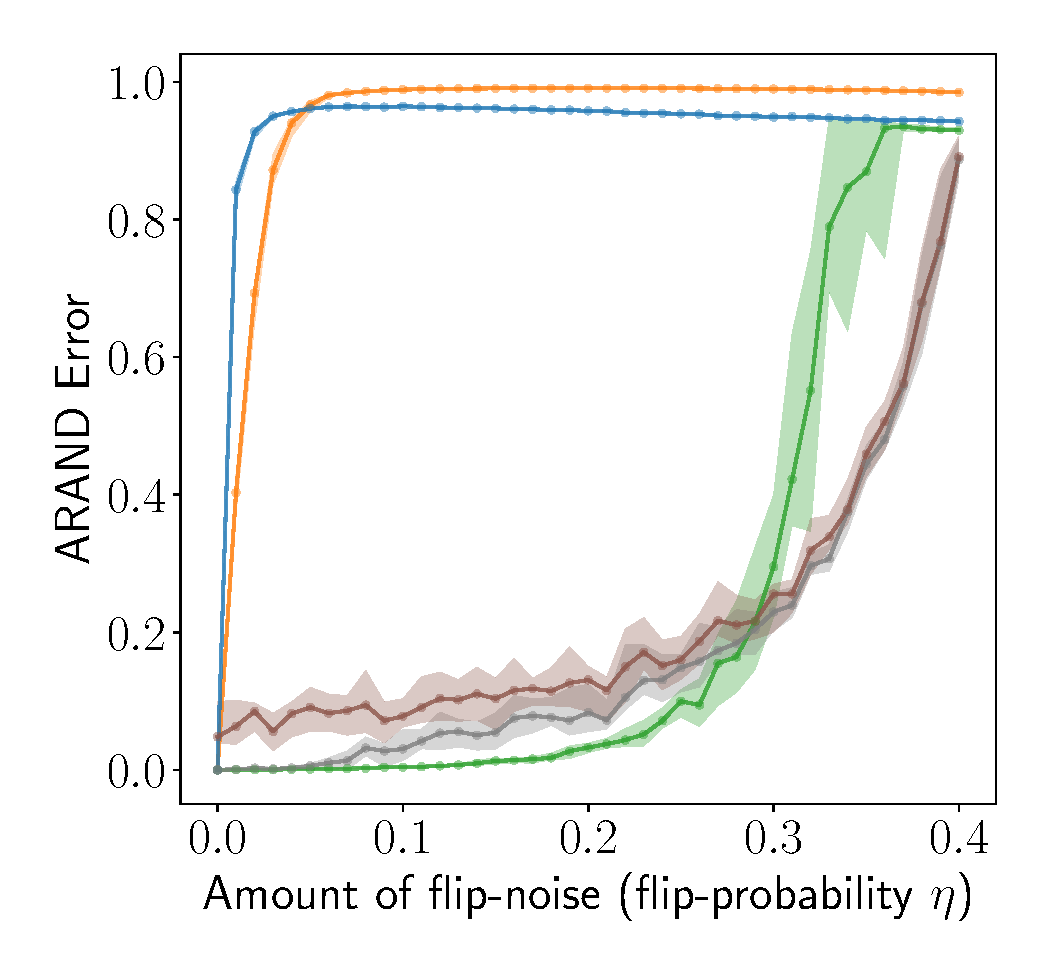
\includegraphics[width=\textwidth,trim=0.34in 0.34in 0.34in 0.34in,clip]{./figures/GASP/SSBM_scores/summary_SSBM_experiments_k20.pdf}
\caption{$k=20$, $p=0.1$}
\end{subfigure}\hfill
\begin{subfigure}[t]{0.44\textwidth}
\centering
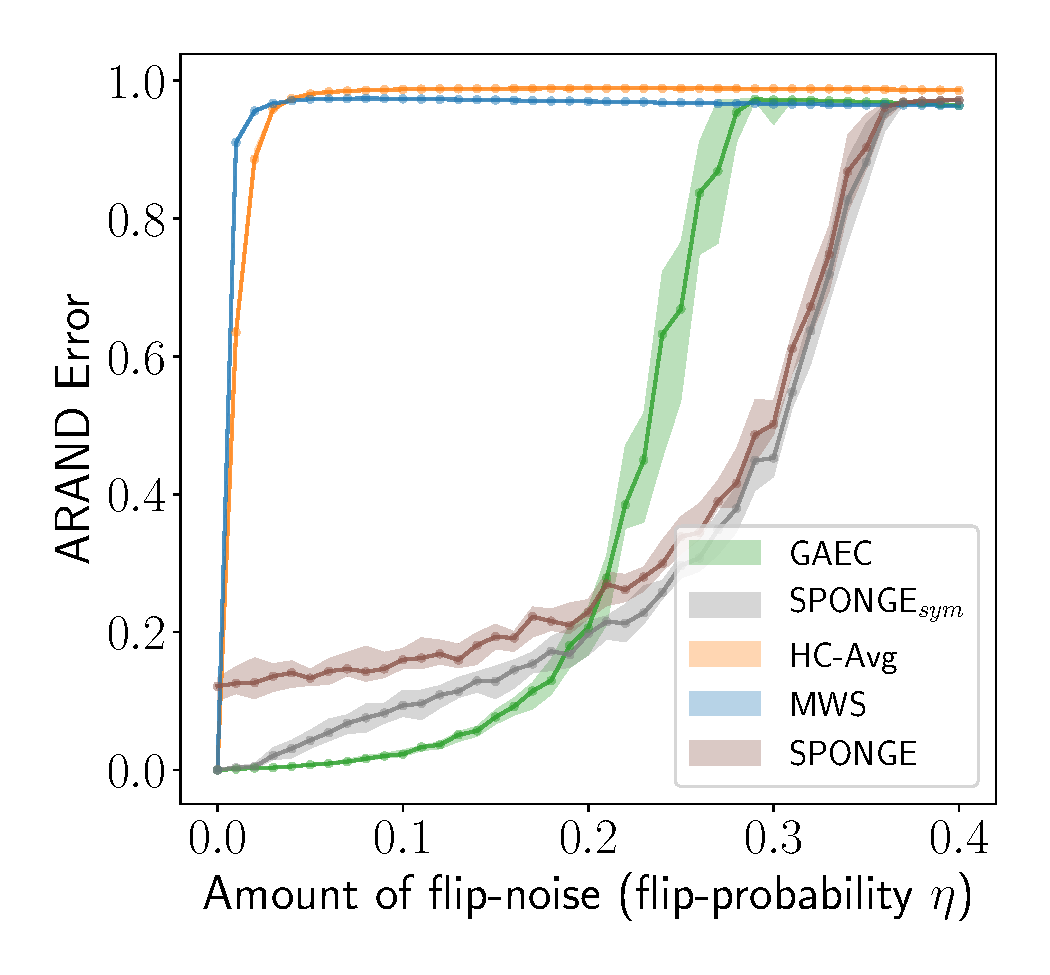
\includegraphics[width=\textwidth,trim=0.34in 0.34in 0.34in 0.34in,clip]{./figures/GASP/SSBM_scores/summary_SSBM_experiments_k50.pdf}
\caption{$k=50$, $p=0.2$}
\end{subfigure}
        \caption{
ARAND errors (median values over 20 experiments, lower is better) on synthetic graphs generated with SSBM. We consider $k$ ground truth communities of random size. Graphs have $N=10000$ nodes and edges are randomly added with probability $p$. 
% The spectral clustering methods, SPONGE and SPONGE$_sym$, were given the true number of clusters as input. 
% Solid lines represent median values over \TODO{30} experiments. Values between the 25th and the 75th percentile are shown in shaded areas.
% We report median, 25th, and the 75th percentile values over \TODO{30} experiments.
%         Scores on SSBM graphs
% \algname{} sensitivity to noise: \emph{Average} linkage proved to be the most robust. Performances are given by Rand-Score (higher is better) depending on the amount of noise added to the CNN predictions.  The two sets of experiments using under- and over-clustering noise are summarized in the plots at the top and at the bottom, respectively (see Appendix \ref{sec:appendix_noise_gen} for more details). For each experiment, some of the long-range CNN predictions were randomly selected with probability $p_{\mathrm{long}}$ and added as long-range edges to the pixel grid-graph. Experiments are performed on a crop of CREMI training sample B.
        } \label{fig:SSBM_scores}
\end{figure}

\begin{table*}[t]
    \centering
    % \scriptsize
    \tiny
    \begin{subtable}[t!]{\textwidth}
    \centering
        \rowcolors{3}{gray!25}{white} % \rowcolors{<starting row index>}{<dispari row color>}{<pari row color>}
        \begin{tabular}{l | r r r r r r r r}
        &\multicolumn{7}{c}{Multicut objective values (average across instances, lower is better)} \\
        Clustering problem & \multicolumn{1}{r}{GAEC \cite{keuper2015efficient}} & HCC-Sum & MWS \cite{wolf2018mutex} & HC-Avg & HCC-Avg & HC-Single & HC-Complete \\ \midrule
        \emph{Modularity Clustering} & 
        -0.457 & -0.453 & -0.073 & \textbf{-0.467} & \textbf{-0.467} & 0.000 & -0.201 \\ 
        \emph{Image Segmentation}  & 
        \textbf{-2,955} & -2,953 & -2,901 & -2,903 & -2,896 & -1,384 &  -2,102 \\
        \emph{Knott-3D (150-300-450)}  & 
        \textbf{-36,667} & -36,652 & -35,200 & -35,957 & -35,631 & -2,522 & 30,629 \\
        \emph{CREMI-3D-rag}  
        & \textbf{-1,112,287} & -1,112,286& -1,109,731 & -1,112,177 & -1,112,100 & -1,038,709 & -748,734,869 \\ 
        \emph{Fruit-Fly Level 1-4}
        & \textbf{-151,022} & -151,017 & -150,879 & -150,909 & -150,876 & -71,477 & -128,733 \\
        \emph{CREMI-gridGraph} 
        & -73,317,601 & -73,328,867 & -73,330,568 & \textbf{-73,502,947} & -73,474,856 & -45,194,180 & 311,598,700 \\
        \emph{Fruit-Fly Level Global} 
        & \textbf{-151,688} & -151,596 & -146,315 & -150,466 & -150,171 & -4,422 & 6,876 \\



        \end{tabular}
    \end{subtable} 
    \caption{We compare algorithms in the \algname{} framework by their value of the multicut objective defined in Eq.~\ref{eq:MC_objective} (lower is better).} 
    \label{tab:energies}
\end{table*}

\begin{figure}[tp]
\centering
% \includegraphics[width=0.48\textwidth,trim=300 100 300 100, clip]{./figures/GASP/dendrograms/new_agglo_order_OLD.png} % left bottom right top
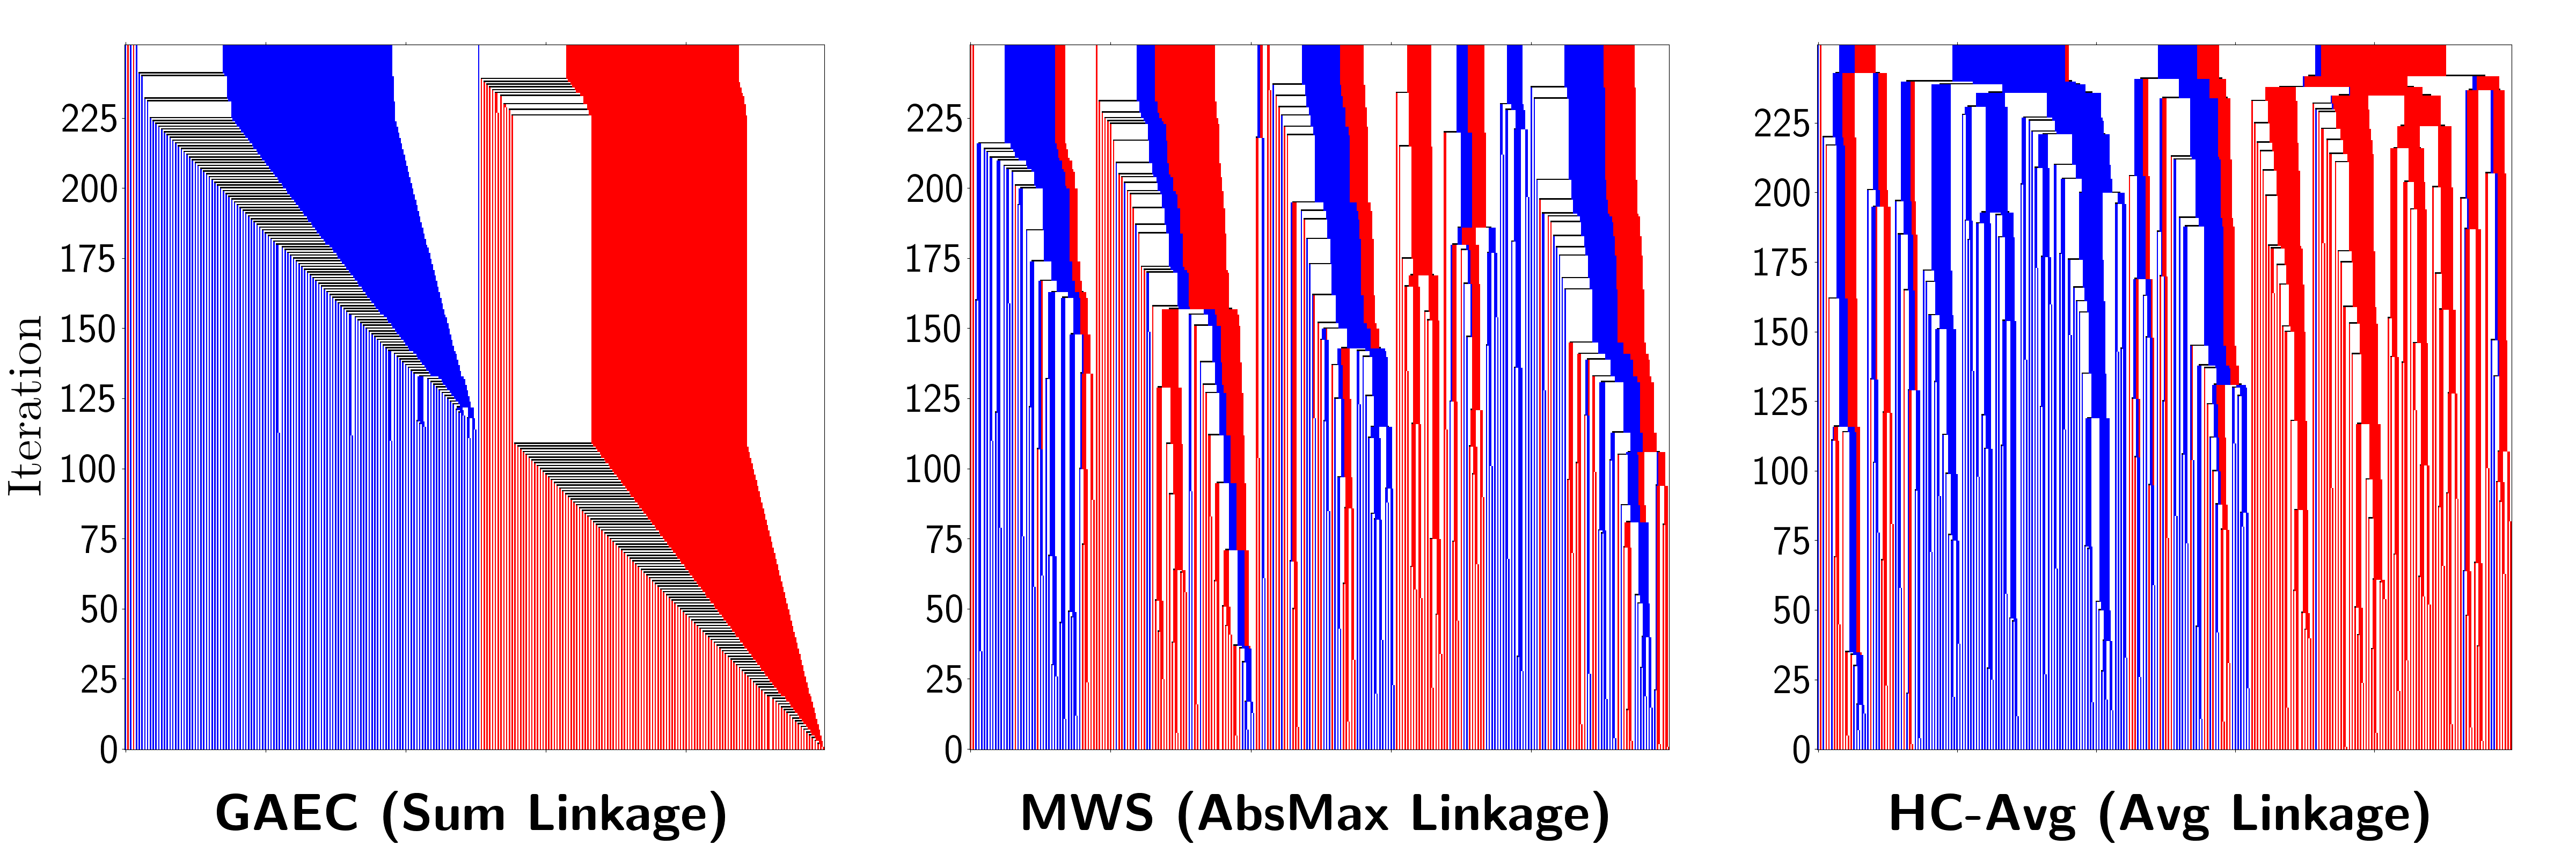
\includegraphics[width=\textwidth,trim=0 10 60 0, clip]{./figures/GASP/dendrograms/new_agglo_order.png} % left bottom right top
\caption{Clustering dynamics and accuracy of GASP variations on stochastic block models. The dendrograms result from three versions of \algname{} on a synthetic graph generated with SSBM ($250$ nodes, edge probability $p=0.05$, flipping probability $\eta=0.1$).  Red and blue colors show which of the two equal-sized ground-truth communities each node belongs to. At the top, dendrograms are truncated at the level of the final clustering $\Pi^*$ returned by \algname{}. \label{fig:dendrograms}}
\end{figure}

\begin{table*}[t]
\centering
% \begin{minipage}[t]{0.48\textwidth}
% \vspace{0pt}
% \centering
\footnotesize
\rowcolors{2}{white}{gray!25} % \rowcolors{<starting row index>}{<dispari row color>}{<pari row color>}
\begin{tabular}[t]{l | c}
\footnotesize
           Method & ARAND Error \\ \midrule
           \textbf{HC-Avg} (GASP with Avg Linkage) & \textbf{0.1034} \\
GAEC \cite{keuper2015efficient} (GASP with Sum Linkage) & 0.1035 \\
MWS \cite{wolf2018mutex} (GASP with AbsMax linkage) & 0.1068 \\
SPONGE$_{sym}$ \cite{Cucuringu2019SPONGEAG} & 0.4161\\
$L_{sym}$ \cite{kunegis2010spectral} & 0.8069 \\
SPONGE \cite{Cucuringu2019SPONGEAG} & 0.9211 \\
BNC \cite{chiang2012scalable} & 0.9926 \\
        \end{tabular}
    \caption{\algname{} compared to spectral clustering methods on a small crop of the CREMI neuron segmentation dataset. 
    Since spectral methods cannot scale to the full CREMI dataset, we evaluated them on a smaller $10\times100\times100$ sub-volume of CREMI training sample B.
    Despite the fact that the true number of ground truth clusters was given as an input to the spectral methods, GASP significantly outperformed them. 
    % SC methods seem to have more difficulties when the graph is sparse. 
    % Spectral methods did not handle well pixels on the boundaries between segments and tended to cluster them together. 
    % We also tried to vary the input number of clusters ncreasing $k$ did not improve their scores either.
% resulting in a graph with $10^5$ nodes and~$\sim10^6$ edges.
    }
    \label{tab:cremi_spectral_experiments}
% \end{minipage}
% \begin{minipage}[t]{0.38\textwidth}
% \vspace{0pt}
% \centering
%         \includegraphics[width=1.\textwidth,trim=0.25in 0.25in 0.68in 0.36in,clip]{./figures/GASP/SSBM_experiments.pdf} % 0.45
%         \caption{\algname{} performances compared to spectral methods on synthetic graphs. The spectral methods were given the true number of clusters as input, in contrast to \algname{}. \TODO{Define paramters SSB; explain percentile stuff (for both noise experiments, save space!)}}
%     \label{fig:SSBM_scores}
% \end{minipage}
\end{table*}


\subsubsection{GASP on synthetic SSBM graphs}   
% can be connected to any  that, depending on the edge-probability parameter $p$, are also \emph{dense}. 
\algname{} algorithms using cannotLinkConstraints are not expected to perform well on these graphs, because of the type of employed sign noise, so we focus our comparison only on the GAEC, HC-Avg and MWS algorithms (using Sum, Average, and AbsMax linkage methods, respectively).
Empirically, we observe that GAEC is the agglomerative algorithm performing best on SSBM graphs, on par with spectral method SPONGE$_{sym}$ (see Fig.~\ref{fig:SSBM_scores}). Given the simple properties of SSBM graphs, we can now give a detailed explanation of these empirical results. 
In SSBM graphs, the number of edges $E_{ij}\equiv(S_i\times S_j)\cap E$ connecting two clusters $S_i,S_j$ is  proportional to the product $|S_i|\cdot|S_j|$ of cluster sizes. 
With Sum or Avg linkage methods, due to the law of large numbers, the flipping noise is ``averaged out'' as soon as the set $E_{ij}$ becomes larger and clusters grow in size.
On the other hand, when clusters are small, it can happen that, for few clusters, several of their edges in $E_{ij}$ are flipped and the algorithm makes a mistake by merging two clusters belonging to different ground truth communities. From this observation, it follows that the \emph{flooding strategy} of the sum-linkage algorithm GAEC is a very good strategy on these types of graphs, because clusters are immediately grown in size (see dendrograms in Fig.~\ref{fig:dendrograms}). Average linkage method HC-Avg instead performs much worse on these graphs because it grows small equally-sized clusters and makes several wrong merge-decisions at the beginning. 
% This observation also explains the empirical results of \cite{chehreghani2020hierarchical}, which involved graph instances with very similar structure to the ones considered here. 
Lastly, the MWS algorithm is not expected to perform well on these graphs because of the high sensitivity of the AbsMax linkage to flipping noise. In the following Proposition \ref{prop:MWS_on_SSBM}, we prove that, at every iteration, the MWS algorithm makes a mistake with at least probability $\eta$, independently on the sizes of the two clusters that are popped from priority queue. In summary, for the SSBM, we can obtain a deep understanding of the dynamics induced by various linkage criteria, and find that GAEC gives highest accuracy by a large margin.
\begin{prop} \label{prop:MWS_on_SSBM}
Consider a graph generated by an Erd\H os-R\'enyi signed stochastic block model (SSBM) as described in Section \ref{sec:clustering_problems}, with $N$ nodes, edges added with probability $p$, sign-flip probability $\eta<0.5$, $k$ ground-truth clusters, and edge weights Gaussian-distributed with standard deviation $\sigma$. Then, at every iteration, \algname{} with Absolute Maximum linkage (or, in other words, the Mutex Watershed algorithm) always makes a mistake with at least probability $\eta$. 
\end{prop}
\begin{proof}
Thanks to Lemma \ref{lemma:absMax_and_complete_property} we know that \algname{} with Absolute Maximum linkage returns the same clustering whether or not cannot-link-constraints are used. Thus, in the following, we prove the proposition considering the version enforcing constraints.
Let us consider a generic iteration of the algorithm, where two clusters $S_\alpha$ and $S_\beta$ have the highest priority and are popped from priority queue. Then, the MWS algorithm will either merge or constrain them depending on the fact that their interaction $\interact_{\mathrm{AbsMax}}(S_\alpha,S_\beta)$ is  positive or negative (note that, with AbsMax linkage, an interaction can never be positive and constrained, as shown in Lemma \ref{lemma:absMax_and_complete_property}).
By construction of the SSBM, every edge $e\in E$ in the graph has a absolute weight distributed as $|w_e|\sim \mathcal{N}(1,\sigma^2)$. Thus, every edge $e'\in(S_{\alpha} \times S_{\beta})\cap E$ connecting the two clusters has the same probability to have the highest absolute weight, and the sign of the interaction $\interact_{\mathrm{AbsMax}}(S_\alpha,S_\beta)$ will only depend on the sign of this highest edge. Therefore, the probability that the MWS merges two clusters is simply given by the fraction of positive weighted edges connecting them.

Let $\tilde{\Pi}=\{\tilde{S}_1,\ldots,\tilde{S}_k\}$ denote the ground truth clustering, and $\tilde{S}_{\alpha i}=S_\alpha\cap \tilde{S}_i$ denote the intersection between cluster $S_{\alpha}$ and a ground-truth cluster $\tilde{S}_i$.
If the generated graph is dense, i.e. $p=1$, then the total number of edges connecting clusters $S_{\alpha}$ and $S_{\beta}$ that have a true attractive or repulsive weight is (according to the ground truth labels)
\begin{equation}
\NBE^+=\sum_{i=1}^k |\tilde{S}_{\alpha i}||\tilde{S}_{\beta i}|, \quad\quad\quad \NBE^-=\sum_{i=1}^k \sum_{j=1,j\neq i}^k |\tilde{S}_{\alpha i}||\tilde{S}_{\beta j}|.
\end{equation}
When the edges in the graph are randomly added with a probability $p$, then the actual number of true attractive and repulsive interactions connecting the two clusters is (according to the ground truth labels):
\begin{equation}
\nBE^+ \sim \mathcal{B}(\NBE^+,p), \qquad \nBE^- \sim \mathcal{B}(\NBE^-,p), 
\end{equation}
where $\mathcal{B}(\NBE,p)$ is the binomial distribution:
\begin{equation}
\mathcal{B}(\nBE;\NBE,p) = \frac{\NBE !}{\nBE! (\NBE-\nBE)!} p^\nBE (1-p)^{\NBE-\nBE}.
\end{equation}
Here, we only assume that $\nBE^+ + \nBE^- >0$, i.e. there is at least one edge connecting the two clusters (otherwise their interaction would be zero and the MWS would not have popped them from priority queue). 

So far we have been talking about attractive and repulsive connections according to the ground truth labels. In our SSBM however every edge has a uniform probability $\eta$ to have its sign flip, so  the actual number of attractive interactions connecting the two clusters will be instead given by the sum of the true attractive interactions $\nBE^+_{\mathrm{nf}}\sim \mathcal{B}(\nBE^+,1-\eta)$ that have not been flipped, plus the true negative interactions $\nBE^-_{\mathrm{f}}\sim \mathcal{B}(\nBE^-,\eta)$ that have been flipped.
Putting everything together, given two clusters with $\nBE^+$ true attractive interactions and $\nBE^-$ true negative ones, the highest-absolute-weight edge connecting them has the following probability to be positive:
\begin{align}\label{eq:mws_prob}
 \mathbb{P}[\interact_{\mathrm{AbsMax}}(S_\alpha,S_\beta)>0;\nBE^+,\nBE^-] = &\, \sum_{\nBE^+_{\mathrm{nf}}=0}^{\nBE^+}\sum_{\nBE^-_{\mathrm{f}}=0}^{\nBE^-} 
\mathcal{B}(\nBE^-_{\mathrm{f}};\nBE^-,\eta) \mathcal{B}(\nBE^+_{\mathrm{nf}};\nBE^+,1-\eta) \cdot \left(\frac{\nBE^+_{\mathrm{nf}}+\nBE^-_{\mathrm{f}}}{\nBE^+ + \nBE^-} \right) \nonumber\\
\stackrel{(*)}{=}&\,\frac{\nBE^+(1-\eta)+\nBE^-\eta}{\nBE^+ + \nBE^-}
\end{align}  
where in $(*)$ we used the fact that the expected value of a binomial distribution $\mathcal{B}(\nBE,\eta)$ is $\nBE \eta$.

%Now we note that this probability is always bounded in the interval $[\eta, 1-\eta]$ (or $[1-\eta, \eta]$, if $\eta>0.5$). Remarkably, these lower and upper bounds do not depend on the number of edges connecting the two clusters, i.e. $\nBE^+ + \nBE^-$ (and, thus, on the sizes of the two clusters). 
Now we note that this probability is bounded in the interval $[\eta, 1-\eta]$. So, regardless of whether the two clusters $S_\alpha$ and $S_\beta$ should be merged or constraint according to ground truth labels, the probability not to make the correct decision is always at least $\eta$.
% So weather we consider a merge or a split of the two clusters as the correct decision, in both cases the expected probability to not make that decision is at least $\eta$. Notably while the exact probabilities depend on the cluster sizes, the lower bound does not. This confirms the intuition that the MWS, unlike Sum or Avg linkage methods, cannot properly correct for sign flip noise by agglomerating larger boundaries and profiting from the law of large numbers. 
Remarkably, while the exact probability in Eq.~\ref{eq:mws_prob} depends on the number of edges connecting the two clusters $\nBE^++\nBE^-$ and thus on the cluster sizes, the bounds do not. Thus, this result shows that, unlike Sum or Avg linkage methods, the MWS algorithm is unable to reliably correct for the sign flip noise even for big clusters linked by many edges.
\end{proof}





\begin{table}[tp]
        \centering
\small
% \begin{minipage}[t]{0.6\textwidth}
%     \centering
        \begin{subtable}[t]{\textwidth}
        \centering
        \rowcolors{3}{gray!25}{white}
        \begin{tabular}[t]{l c c c c}
        \toprule
          & ARAND & VOI & VOI&  Runtime \\ 
          & Error & split & merge&  (s) \\ \midrule 
\textbf{HC-Avg} & \textbf{0.0487} & 0.387 & 0.258 & 2344 \\
HCC-Avg & 0.0492 & 0.389 & 0.259 & 2892 \\
MWS \cite{wolf2018mutex} & 0.0554 & 0.440 & 0.249 & 688 \\
GAEC \cite{keuper2015efficient} & 0.0856 & 0.356 & 0.338 & 4717 \\
HCC-Sum & 0.0872 & 0.365 & 0.337 & 4970 \\
% HCC-Complete & 0.9206 & 4.531 & \textbf{0.210} & 1330 \\
HC-Complete & 0.9211 & 4.536 & \textbf{0.211} & 1020 \\
HC-Single & 0.9264 & \textbf{0.060} & 4.887 & \textbf{312} \\
HCC-Single & 0.9264 & \textbf{0.060} & 4.887 & 6440 \\
        \end{tabular}
    % \captionof{table}{CREMI-Scores achieved by different linkage criteria and thresholding. All methods use the affinity predictions from our CNN as input. Scores are averaged over the three CREMI training datasets.}
    \caption{\centering CREMI-gridGraph (OurCNN)}
    \vspace*{2.5em}
    \label{tab:scores_gridGraph}
    \end{subtable}
\begin{subtable}[t]{\textwidth}
\centering
\rowcolors{3}{gray!25}{white} % \rowcolors{<starting row index>}{<dispari row color>}{<pari row color>}
        \begin{tabular}[t]{@{\hspace{0.7\tabcolsep}}l c @{\hspace{1\tabcolsep}} c @{\hspace{1.1\tabcolsep}} c @{\hspace{1\tabcolsep}} c @{\hspace{1\tabcolsep}}}
        \toprule
        % \rowcolor{gray!50}
          & ARAND & VOI & VOI&  Runtime \\ 
          % \rowcolor{gray!50}
          & Error & split & merge&  (s) \\ \midrule 
\textbf{HC-Avg} & \textbf{0.0896} & 0.603 & 0.323 & 86 \\
HCC-Avg & 0.0898 & 0.600 & 0.325 & 87 \\
GAEC \cite{keuper2015efficient} & 0.0905 & 0.606 & 0.323 & 89 \\
HCC-Sum & 0.0910 & 0.608 & 0.323 & \textbf{85} \\
MWS \cite{wolf2018mutex} & 0.1145 & 0.825 & 0.295 & 86 \\
HCC-Single & 0.5282 & \textbf{0.437} & 1.367 & 88 \\
HC-Single & 0.5282 & \textbf{0.437} & 1.367 & \textbf{85} \\
% HCC-Complete & 0.5564 & 2.220 & 0.254 & 89 \\
HC-Complete & 0.5654 & 2.253 & \textbf{0.249} & 86 \\
        \end{tabular}
        % \hspace*{5em}
    \caption{\centering CREMI-3D-RAG (OurCNN)}
    \vspace*{2.5em}
    \label{tab:scores_3drag}
    \end{subtable}

    \begin{subtable}[t]{\textwidth}
    % \end{table}
% \end{minipage}\hfill
% \begin{minipage}[t]{0.38\textwidth}
    \centering
    \rowcolors{3}{gray!25}{white} % \rowcolors{<starting row index>}{<dispari row color>}{<pari row color>}
        \begin{tabular}[t]{l @{\hspace{1.2\tabcolsep}} c @{\hspace{1\tabcolsep}} c @{\hspace{1\tabcolsep}} c @{\hspace{0.8\tabcolsep}} c @{\hspace{1\tabcolsep}} c}
        % \begin{tabular}[t]{lcccc}
        \toprule
        & Needs & CREMI& ARAND & VOI & VOI\\ 
          & superpixels? & Score & Error & split & merge\\ \midrule 
          % & \makecell{CREMI\\Score} & \makecell{ARAND\\error} & \makecell{VOI\\split} & \makecell{VOI\\merge}    \\ \midrule 
OurCNN: 3D-RAG + LiftedMulticut & \CrossedBox & \textbf{0.221} & \textbf{0.108} & \textbf{0.339} & 0.115 \\
\emph{GASP: OurCNN + gridGraph + HCC-Avg} & \HollowBox & 0.224 & 0.113 & 0.361 & 0.085  \\
\emph{GASP: OurCNN + gridGraph + HC-Avg}  & \HollowBox &0.224 & 0.114 &  0.364 & 0.083 \\
PNI CNN \cite{lee2017superhuman} & \CrossedBox &0.228 & 0.116 & 0.345 & 0.106 \\
LSI-Masks \cite{bailoni2020proposal}  & \HollowBox &0.246 & 0.125 & 0.383 & 0.107  \\
\emph{GASP: OurCNN + 3D-RAG + HCC-Avg} & \CrossedBox &0.257 & 0.132 & 0.438& \textbf{0.063} \\  
\emph{GASP: OurCNN + 3D-RAG + HC-Avg} & \CrossedBox &0.262 & 0.135 & 0.448 & \textbf{0.063}   \\  
% \textbf{Our CNN + \algname{} Average} & \textbf{0.241 \\
MALA CNN + MC \cite{funke2018large} & \CrossedBox & 0.276  & 0.132 &0.490  & 0.089  \\
CRU-Net \cite{zeng2017deepem3d} & \CrossedBox &0.566 & 0.229 & 1.081 &  0.389    \\
% LFC \cite{parag2017anisotropic} & 0.616 & 0.313 & 1.085 & 0.140     \\
        \end{tabular}
        \caption{\centering CREMI Challenge leader-board}
        \vspace*{1.5em}
        \label{tab:cremi_leaderboard}
        \end{subtable}
        % \vspace*{0.99em}
    % \captionof{table}{Current leading entries  in the CREMI challenge leaderboard \cite{cremiChallenge} (March 2021)}
    % \label{tab:results_cremi_test}
    \caption{\textbf{(a-b)}: Scores and run times of algorithms in the \algname{} framework on the \emph{CREMI-gridGraph} and \emph{CREMI-3D-RAG} clustering problems: average linkage methods achieved the best accuracy. Measures shown are: Adapted-Rand error (ARAND, lower is better); Variation of Information (VOI) \cite{arganda2015crowdsourcing} (VOI-merge for under-clustering error and VOI-split for over-clustering error, lower values are better). \textbf{(c)}: Current leading entries in the CREMI challenge leaderboard. CREMI-score is given by the geometric mean of (VOI-split + VOI-merge)  and ARAND error (lower is better).}
    \label{tab:scores}
% \end{minipage}
\end{table}
\begin{figure}[tp]
\centering
\includegraphics[width=\textwidth,trim=0 10 60 0, clip]{./figures/GASP/comparison_GAEC_MWS_Avg.png} % left bottom right top
\caption{Failure cases of three versions of \algname{} applied to neuron segmentation. Only \emph{wrongly} segmented regions are highlighted in different warm colors. Red arrows point to wrongly split regions; yellow arrows point to false merge errors. HC-Avg returned the best segmentation. Data is 3D, hence the same color could be assigned to parts of segments that appear disconnected in 2D.  
\label{fig:failure_cases}}
\end{figure}
\begin{figure}[tbp]
\centering
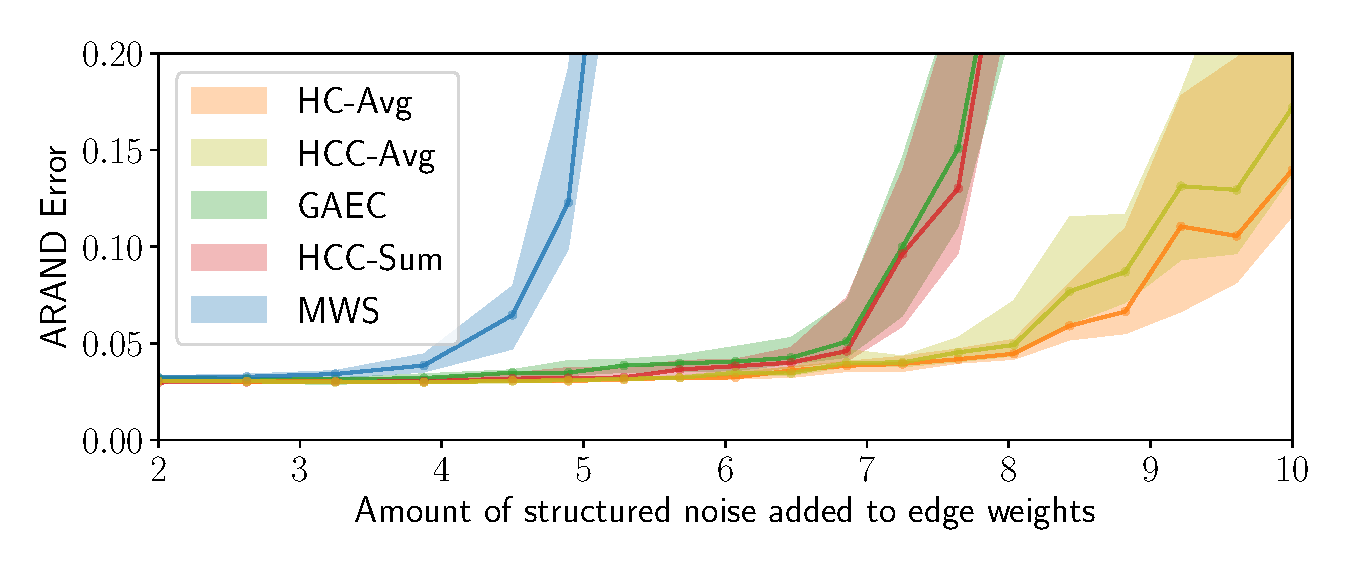
\includegraphics[width=0.87\textwidth,trim=0.2in 0.17in 0.2in 0.2in,clip]{./figures/GASP/noise_plots_adapted-rand_1.pdf}
        \caption{
ARAND errors (median values over 20 experiments, lower is better) on \emph{CREMI-gridGraph} clustering problems perturbed with structured noise. Average-linkage algorithms proved to be the most robust.
% We report median, 25th, and the 75th percentile values over \TODO{30} experiments.
% \algname{} performances compared to spectral methods on synthetic graphs. The spectral methods were given the true number of clusters as input, in contrast to \algname{}. \TODO{Define paramters SSB; explain percentile stuff (for both noise experiments), user ARAND-error}
}\label{fig:scores_structured_noise}
\end{figure}


\subsubsection{GASP on neuron segmentation graph instances}
SSBM graphs are \emph{non-planar}, and every edge has the same probability to be present in the graph. On the other hand, the \emph{gridGraph} and \emph{3D-RAG} graphs of Table~\ref{tab:datasets} are sparse and have a very regular structure: regardless of whether a node represents a pixel or a superpixel, it will only have edge connections with its neighbors in the image (up to a certain hop distance). 
Tables~\ref{tab:scores_gridGraph}-\ref{tab:scores_3drag} show that average linkage methods (HC-Avg, HCC-Avg) strongly outperform other methods on \emph{CREMI-gridGraph} instances and also achieve the best scores on \emph{CREMI-3D-rag} graphs. Sum-based linkage methods (GAEC, HCC-Sum) have a two times higher ARAND error on grid-graphs and often return under-clustered segments (see failure cases in Fig.~\ref{fig:failure_cases}). This suggests that the \emph{flooding strategy} observed previously in the sum-linkage methods does not work on grid-graphs, because in this setup edge weights are predicted by a CNN and noise is strongly spatially-correlated \footnote{This effect is not as strong on \emph{3D-RAG} graphs, because edge weights are computed by averaging CNN predictions (and noise) over the boundaries of adjacent supervoxels.}.
To fully test this hypothesis, we conduct a set of experiments where the CNN predictions are perturbed by adding structured noise and simulating additional artifacts like ``holes'' in the boundary evidence\footnote{See Appendix \ref{sec:appendix_noise_gen} for details about how we perturbed the \emph{CREMI-gridGraph} problems by using Perlin noise \cite{perlin2001noise,perlin1985image}, which is one of the most common gradient noises used in procedural pattern generation.}. 
The plot in Fig.~\ref{fig:scores_structured_noise} confirms that HC-Avg and HCC-Avg are very robust algorithms on this data, followed by Sum-linkage algorithms and the Mutex Watershed algorithm (MWS). It is not a surprise that the AbsMax linkage used by MWS is not robust to this type of structured noise. However, the scores and runtimes in Table~\ref{tab:scores_gridGraph} prove how MWS can achieve high accuracy with 70\% lower runtime compared to HC-Avg. 

\paragraph{Complete and Single Linkage} We use these two linkage methods as baselines to highlight the difficulty of the studied graph clustering problems listed in Table~\ref{tab:datasets}. Scores in Tables~\ref{tab:scores_gridGraph}-\ref{tab:scores_3drag} show their poor performance: Single linkage hierarchical clustering (HC-Single), which here is equivalent to thresholding the edge weights at $w_e=0$ and computing connected components in the graph, often returned few big under-segmented clusters. HC-Complete returned instead a lot of over-segmented clusters. 
% These algorithms are excluded from our next comparison experiments.








\paragraph{Results on CREMI challenge} 
Table~\ref{tab:cremi_leaderboard} shows that the HCC-Avg and HC-Avg clustering algorithms achieve state-of-the-art accuracy on the CREMI challenge, when combined with predictions of our CNN.
Most of the other entries (apart from \emph{LSI-Masks} \cite{bailoni2020proposal}) employ super-pixels based post-processing pipelines and cluster 3D-region-adjacency graphs. As we show in Table ~\ref{tab:scores_3drag}, using superpixels considerably reduces the size of the clustering problem and, consequently, the post-processing time. 
However, our method operating directly on pixels (\emph{gridGraph + HCC-Avg}) achieves better performances than superpixel-based methods (\emph{3D-RAG + HCC-Avg}) and does not require the parameter tuning necessary to obtain good super-pixels, which is usually highly dataset dependent.
To scale up our method operating on pixels, we divided each test-volume into four sub-blocks, and then combined the resulting clusterings by running the algorithms again on the combined graph.
The method \emph{3D-RAG + LiftedMulticut} based on the lifted multicut approximation of \cite{beier2017multicut} achieves the best scores overall, but it takes into account different information through the lifted edge weights that also depend on additional raw-data and shape information from highly engineered super-pixels. 
% Note that the test volumes of the challenge contain several imaging artifacts that make segmentation particularly challenging.
% However: handcrafted and dataset dependent, performs better, no

% Given By building a grid-graph from our CNN predictions  and solving a clustering problem with the \emph{HCC-Avg} and \emph{HC-Avg} algorithms, representing the best performing algorithms included in the proposed \algname{} framework, we achieve state-of-the-art performances on the competitive CREMI challenge (see Table~\ref{tab:cremi_leaderboard}). 

% To scale up the pixel-based aggSpecify that we divided samples into four blocks and then run the agglomeration again (moreover, run seeded WS to get rid of small segments).

% then \algname{} with cannot-link constraints shows a clear tendency to over-cluster. \\

% Superpixels are nice because they reduce runtime and represents the standard choices for connectomics (all bug LSI-Masks use some kind of similar form). But method is very dataset-dependent and require the user to set a series of parameters

% So far no other method was done from pixels







% The competitive performance of this simple parameter-free algorithm is also reported in Table \ref{tab:results_cremi_test}, showing the current leader-board of the challenge: 


% Note that the test volumes contain several imaging artifacts that make segmentation particularly challenging. 
% and might profit from more robust edge statistics of super-pixel based approaches.

% and can also avoid errors that result from wrong superpixels that cannot be fixed during later agglomeration.
% In Appendix \ref{sec:appendix_exps_full_cremi}, we provide more details about how we scaled up \algname{} to the full datasets. 
% Appendix Table \ref{tab:extended_results_cremi} lists the performances and the run-times for all tested \algname{} linkage criteria.\\


% We first evaluate and compare the agglomerative clustering algorithms described in the generalized framework on the task of neuron segmentation in electron microscopy (EM) image volumes. This application is of key interest in connectomics, a field of neuro-science with the goal of reconstructing neural wiring diagrams spanning complete central nervous systems. Currently, only proof-reading or manual tracing yields sufficient accuracy for correct circuit reconstruction \cite{schlegel2017learning}, thus further progress is required in automated reconstruction methods.

% EM segmentation is commonly performed by first predicting 
% boundary pixels \cite{beier2017multicut,ciresan2012deep} or undirected affinities \cite{wolf2018mutex,lee2017superhuman,funke2018large}, which represent how likely it is for a pair of pixels to belong to the same neuron segment. 
% The affinities do not have to be limited to immediately adjacent pixels.
% Thus, similarly to \cite{lee2017superhuman}, we train a CNN to predict both short- and long-range affinities
% and use them as edge weights of a 3D grid graph, where each node represents a pixel/voxel of the volume image. 



% % % !TEX root = ../agglo_clust_review.tex


% \captionsetup[subtable]{labelformat=simple, labelsep=space, justification=centering, singlelinecheck=off}
% \renewcommand*{\thesubtable}{(\alph{subtable})}
% \begin{table}[t]
% \centering
% \begin{subtable}{0.5 \textwidth}
%     \centering
%     \scriptsize
%         \begin{tabular}{l|l|cc}
%             Method & Agglomeration type & AP \\ \midrule
%             PANet \cite{liu2018path} & - & \textbf{36.5} \\
%             Mask R-CNN \cite{he2017mask} & - & 31.5 \\ \hline
%              & \algname{} Average& 34.3 \\
%              & \algname{} Average + Constraints & 33.9 \\
%             \multirow{2}{*}{GMIS Model \cite{liu2018affinity}} & MultiStepHAC \cite{liu2018affinity} & 33.0 \\
%              & \algname{} Abs. Max. \cite{wolf2018mutex}  & 32.1 \\
%              & \algname{} Sum + Constraints  \cite{levinkov2017comparative} & 31.9  \\
%              & \algname{} Sum \cite{keuper2015efficient} & 31.3 \\
%         \end{tabular}
%     \caption{CityScapes \emph{validation} set}
%     \label{tab:results_cityscapes_val}
% \end{subtable}\hfill
% \begin{subtable}{0.46\textwidth}
% \centering
%     \scriptsize
% \begin{tabular}{l|cc}
%            Method & AP  & AP 50\% \\ \midrule
%            Panoptic-DeepLab \cite{cheng2019panopticdeeplab} & 34.6 & 57.3 \\
%            UPSNet \cite{xiong2019upsnet} $\dagger$ & 33.0 & 59.6 \\
%            SSAP \cite{Gao_2019_ICCV} & 32.7 & 51.8 \\
%            PANet \cite{liu2018path} $\dagger$ & 31.8 & 57.1 \\
%            \textbf{GMIS Model + \algname{} Average} & \textbf{28.3} & \textbf{47.0} \\ 
%            JOSECB \cite{neven2019instance} & 27.7 & 50.9 \\
%            GMIS \cite{liu2018affinity} & 27.3 & 45.6 \\
%            Mask R-CNN \cite{he2017mask} $\dagger$ & 26.2 & 49.9 \\
%            SGN \cite{liu2017sgn} & 25.0 & 44.9 \\
%            DIN \cite{arnab2017pixelwise} & 20.0 & 38.8 \\
%            DWT \cite{bai2017deep} & 19.4 & 35.3 \\
%            InstanceCut \cite{kirillov2017instancecut} & 13.0 & 27.9 \\
%         \end{tabular}
%     \caption{CityScapes \emph{test} set}
%     \label{tab:results_cityscapes_test}
% \end{subtable}
% \caption{Average Precision scores (higher is better) on the CityScapes dataset. \algname{} with \emph{Average} linkage combined with the GMIS Model \cite{liu2018affinity} represents the proposal-free method achieving the best results (May 2019). In order to have a fair comparison, we only compare methods that did not use external data (e.g. COCO \cite{lin2014microsoft}) for training. In Table (a) we distinguish between proposal-based and proposal-free methods.}\label{tab:results_cityscapes}
% \end{table}



\section{Experiments on CityScapes}\label{sec:cityscapes_exp}
\TODO{In case, I need to define again bias $\beta$}
The segmentation performance of \algname{} is evaluated on the CityScapes dataset \cite{cordts2016cityscapes}, which consists of 5000 street-scene images.
Several of the current top instance segmentation methods on cityscapes predict affinities, e.g. SSAP \cite{Gao_2019_ICCV} and GMIS \cite{liu2018affinity}. 
Since \cite{liu2018affinity} made the code and model publicly available, we used their pipeline consisting of two CNNs with similar architectures (one predicting semantic scores and the other pixel affinities between instances) and applied all the post-processing methods proposed by them, e.g. excluding background and resizing regions of interest. We then provided the output instance-affinities of the model as input to \algname{}. 
In \cite{liu2018affinity} the instance-branch of the model was trained with a Binary Cross-Entropy loss, but we noticed how strong short-range boundary evidence was never predicted by the model. In Appendix \ref{sec:appendix_cityscapes} we present how we solved this problem by fine-tuning the model with \emph{S\o resen-Dice} loss, similarly to \cite{wolf2018mutex}. Finally, the semantic categories were assigned to each instance by a majority vote based on the semantic output. 

Results on the \emph{test} set are summarized in Table \ref{tab:results_cityscapes_test}. The best scores are achieved by Panoptic-DeepLab \cite{cheng2019panopticdeeplab} that proposes a more powerful CNN model to regress the centers of the instances. The second best \emph{proposal-free} method is SSAP \cite{Gao_2019_ICCV}, which predicts long-range instance-affinities similarly to GMIS \cite{liu2018affinity}, but trains the model with extra side-losses. \algname{} with \emph{Average} linkage also achieves competitive results and outperforms the previous agglomeration method proposed in GMIS \cite{liu2018affinity}. Similarly to the experiments on neuron segmentation, results on the \emph{val} set (see Table \ref{tab:results_cityscapes_val} and Fig. \ref{fig:cityscapes}) show that other \algname{} linkage criteria tend to over-cluster, e.g. \emph{Abs Max}, or under-cluster and merge instances, e.g. \emph{Sum}. The graph-merging algorithm proposed by \cite{liu2018affinity} (MultiStepHAC) requires the user to tune several threshold parameters and when we applied it to the affinities predicted by our fine-tuned model it achieved an AP score of 33.0 on the \emph{val} set, which is worse than the original value 34.1 reported in \cite{liu2018affinity}. This is probably due to the fact that MultiStepHAC was tailored to the output affinities of the original model. 
Table \ref{tab:extended_results_cityscapes_val} in Appendix includes the scores of all other tested \algname{} algorithms.

% \captionsetup[subtable]{labelformat=simple, labelsep=space, justification=centering, singlelinecheck=off}
\renewcommand*{\thesubtable}{(\alph{subtable})}
\begin{figure}[t]
\centering
\begin{minipage}[t]{0.48 \textwidth}
\vspace{0pt}
\centering
\small
\begin{tabular}[t]{l|cc}
     Agglomeration method & AP \\ \midrule
    % PANet \cite{liu2018path} & - & \textbf{36.5} \\
    % Mask R-CNN \cite{he2017mask} & - & 31.5 \\ \hline
      \textbf{\algname{} Average}& \textbf{34.3} \\
      \algname{} Average + Constraints & 33.9 \\
     MultiStepHAC \cite{liu2018affinity} & 33.0 \\
      \algname{} Abs. Max. \cite{wolf2018mutex}  & 32.1 \\
      \algname{} Sum + Constraints  \cite{levinkov2017comparative} & 31.9  \\
      \algname{} Sum \cite{keuper2015efficient} & 31.3 
\end{tabular}
\vspace*{1.5em}
\captionof{table}{Average Precision scores on CityScapes \emph{val} achieved by the GMIS Model trained in \cite{liu2018affinity} and different graph agglomeration methods.}
\label{tab:results_cityscapes_val}
\end{minipage}\hfill
\begin{minipage}[t]{0.49\textwidth}
% \centering
\scriptsize
\begin{tabular}[t]{l|cc}
    \multirow{2}{*}{Method}    & AP  & AP 50\% \\ 
     & \multicolumn{2}{c}{(higher is better)} \\ \midrule
       Panoptic-DeepLab \cite{cheng2019panopticdeeplab} & 34.6 & 57.3 \\
       UPSNet \cite{xiong2019upsnet} $\dagger$ & 33.0 & 59.6 \\
       SSAP \cite{Gao_2019_ICCV} & 32.7 & 51.8 \\
       AdaptIS \cite{sofiiuk2019adaptis} & 32.5 & 52.5 \\
       PANet \cite{liu2018path} $\dagger$ & 31.8 & 57.1 \\
       \textbf{GMIS\cite{liu2018affinity}+\algname{}Average} & \textbf{28.3} & \textbf{47.0} \\ 
       JOSECB \cite{neven2019instance} & 27.7 & 50.9 \\
       \textbf{GMIS} \cite{liu2018affinity} & \textbf{27.3} & \textbf{45.6} \\
       Mask R-CNN \cite{he2017mask} $\dagger$ & 26.2 & 49.9 \\
       SGN \cite{liu2017sgn} & 25.0 & 44.9 \\
       % DIN \cite{arnab2017pixelwise} & 20.0 & 38.8 \\
       % DWT \cite{bai2017deep} & 19.4 & 35.3 \\
       % InstanceCut \cite{kirillov2017instancecut} & 13.0 & 27.9 \\
    \end{tabular}
% \caption{CityScapes \emph{test} set}
% \vspace*{0.6em}
\captionof{table}{Results on CityScapes test. Methods marked with~$\dagger$ are \emph{proposal-based}. Only methods that do not use external training data (such as MS COCO) are shown.}\label{tab:results_cityscapes}
\label{tab:results_cityscapes_test}
\end{minipage}
\end{figure}
\begin{figure}[t]
\centering
\begin{minipage}{0.48\textwidth}
\centering
\includegraphics[width=\textwidth]{./figs/cityscapes_compare_6.pdf} % left bottom right top
\caption{Visual results given by different \algname{} linkage criteria on a crop of a CityScapes image from the \emph{validation} set.}\label{fig:cityscapes}
\end{minipage}
\end{figure}



% !TEX root = ../../main.tex
\section{Conclusion}
We have presented a unifying framework for agglomerative clustering of graphs with both positive and negative edge weights. This framework allowed us to explore new combinations of constraints and linkage criteria and to perform a consistent evaluation of all algorithms in it. 
% and we have shown that some existing clustering algorithms, e.g. the Mutex Watershed, can be reformulated as special cases of this framework. 
We have then analyzed several theoretical and empirical properties of these algorithms. On instance segmentation, algorithms based on an average linkage criterion outperformed all the others: they proved to be simple and robust approaches to process short- and long-range predictions of a CNN.
 % applied to an instance segmentation task.
On biological images, these simple average agglomeration algorithms achieve state-of-the-art results without requiring the user to spend much time tuning complex task-dependent pipelines based on super-pixels.
% can represent a valuable choice for a user who is not willing to spend much time tuning complex task-dependent pipelines based on super-pixels.  
% In future work, we plan to explore common theoretical properties of the algorithms included in the framework.
% On biological images, this simple average agglomeration algorithm superpixels



%--------------------- LSI-Masks ----------------------
% !TEX root = ../../main.tex
\chapter{predicting Latent Single-Instance Masks}\label{chapter:LSI}

In this chapter we introduce a new proposal-free instance segmentation method that builds on single-instance segmentation masks predicted across the entire image in a sliding window style.
In contrast to related approaches, this method concurrently predicts all masks, one for each pixel, and thus resolves any conflict jointly across the entire image.
Specifically, predictions from overlapping masks are combined into edge weights of a signed graph that is subsequently partitioned to obtain all final instances concurrently.
The result is a parameter-free method that is strongly robust to noise and prioritizes predictions with the highest consensus across overlapping masks. 
All masks are decoded from a low dimensional latent representation, which results in great memory savings strictly required for applications to large volumetric images. 
We test our method on the challenging CREMI 2016 neuron segmentation benchmark where it achieves competitive scores. 

\begin{figure}[t]
\centering
        % \includegraphics[width=0.4\textwidth,trim=0.25in 0.25in 0.68in 0.36in,clip]{./figs/SSBM_experiments.pdf} % 0.45
        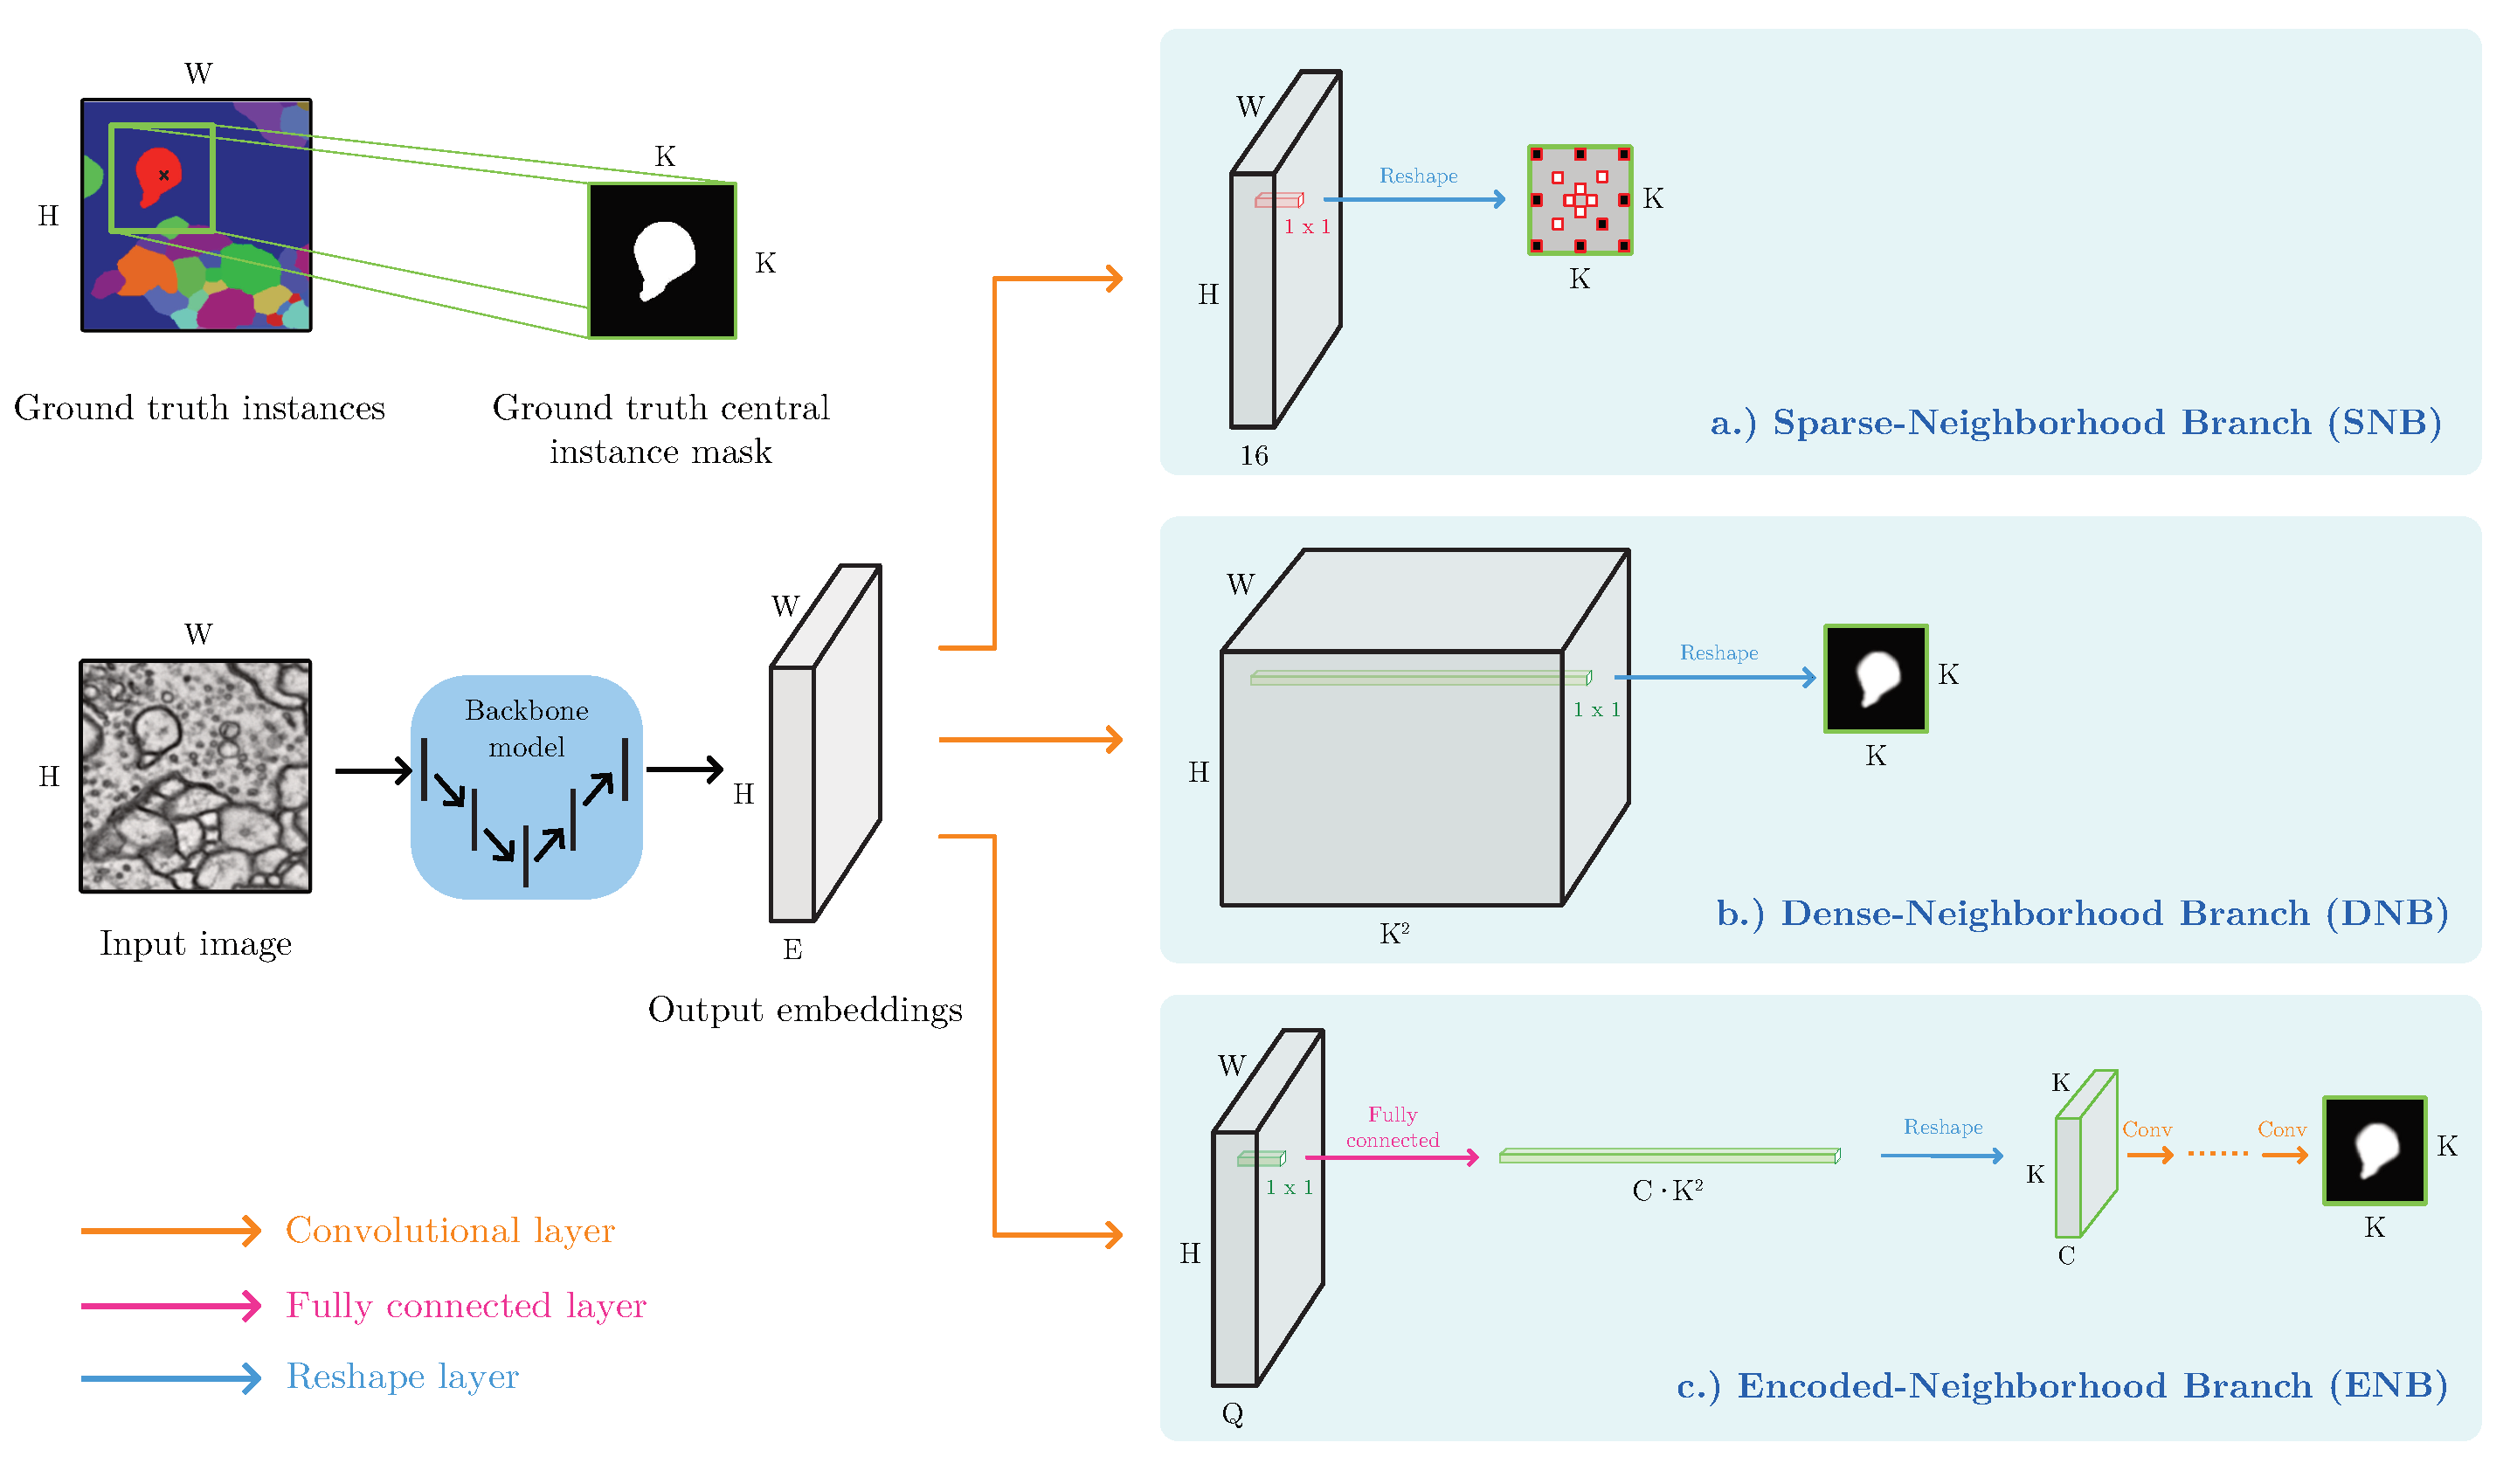
\includegraphics[width=\textwidth]{./figures/LSIMasks/main_fig.pdf} % 0.45
        \caption{Comparison between the proposed method and the strong baseline representing the current state-of-the-art. \textbf{Left}: At the top-left corner, an example of binary \maskname mask for a given ground truth label image; below, the backbone model predicts feature maps with the spatial dimensions of the input image. \textbf{Right}: a.) \emph{Sparse-neighborhood branch} used in the baseline model to predict affinities for a given sparse neighborhood structure; b) Simple generalization of the \emph{\sparseBr branch} to predict dense \maskname masks; c) Proposed \emph{\encBr branch} predicting \maskname masks in a low-dimensional latent space.}
    \label{fig:main_figure}
\end{figure}




\section{Introduction}\label{sec:intro}

\emph{Instance segmentation} is the computer vision task of assigning each pixel of an image to an instance, such as individual car, person or biological cell. %, where the number of instances is usually not known in advance. 
% The most success in instance segmentation (IS) has been achieved by applying deep learning. %\cite{he2017mask,romera2016recurrent,liu2018affinity}. 
There are two main types of successful deep learning approaches to instance segmentation: \emph{proposal-based} and \emph{proposal-free} methods. 
Recently, there has been a growing interest in the latter. Proposal-free methods do not require object detection and are preferred in imagery as studied here, in which object instances cannot be approximated by bounding boxes and are much larger than the field of view of the model.  

 
% A graph partitioning algorithm is used to obtain object instances.
Some recent successful proposal-free approaches \cite{januszewski2018high,liu2016multi,meirovitch2016multi} tackle instance segmentation by predicting, for a given patch of the input image, whether or not each pixel in the patch is part of the instance that covers the central pixel of the patch. 
This results a probability mask, which from now on we call \emph{\maskname mask}. These masks are then repeatedly predicted across the entire image, either in a sliding window style or by starting from a seed and then shifting the field of view depending on the previously predicted masks. 
Final object-instances are then obtained by aggregating predictions from overlapping masks which is in itself a nontrivial and interesting problem.
% In the following, we will refer to these patch predictions as \emph{\maskname masks}.

In this chapter, we introduce a new proposal-free segmentation method that is also based on predicting \maskname masks\footnote{For interesting, closely related but independent work, see \cite{hirsch2020patchperpix}.}.
% \footnote{Note to reviewers: As per ECCV reviewer instructions, there is no need to cite arxiv papers and they are not considered as prior \TODO{state of the art}. However, for maximum transparency and because we appreciate their fine work, we propose to keep footnote (1), hopefully upgraded to a full reference in our camera-ready version.}
However, our approach comes with four main advantages compared to previous methods.
Firstly, our model concurrently predicts all \maskname masks, one for each pixel, by using a fully-convolutional approach with much smaller computational footprint than previous methods, which iteratively predict one instance at the time, one mask after the other \cite{januszewski2018high,meirovitch2016multi}.
Secondly, our approach predicts \maskname masks in a low dimensional latent representation (see Fig. \ref{fig:main_figure}c), which results in great memory savings that are strictly required to apply the method to large volumetric images. 
Thirdly, the proposed approach aggregates predictions from overlapping \maskname masks without the need for any extra parameter or threshold and outputs predictions with associated uncertainty;
and, finally, all final object-instances are obtained concurrently, as opposed to previous methods predicting them one-by-one with subsequent conflict resolution. 
% by extracting a set of affinities that are then used as signed weights of a graph representing the image, so that each node corresponds to a pixel

% Despite the recent successful application of patch-based methods, so far no study has been conducted to compare them with 

Additionally, we systematically compare the proposed model with the current state-of-the-art proposal-free method both on natural and biological images \cite{liu2018affinity,Gao_2019_ICCV,lee2017superhuman,wolf2018mutex,bailoni2019generalized}. This strong baseline consists of a fully-convolutional network predicting, for each pixel, an arbitrary predefined set of short- and long-range affinities, i.e. neighborhood relations representing how likely it is for a pair of pixels to belong to the same object instance (see Fig. \ref{fig:main_figure}a). 

Our method achieves competitive scores on the challenging CREMI 2016 neuron segmentation benchmark. In our set of validation experiments, we show how predicting encoded \maskname masks always improves accuracy. Moreover, when predictions from overlapping masks are combined into edge weights of a graph that is subsequently partitioned, the result is a method that is strongly robust to noise and gives priority to predictions sharing the highest consensus across predicted masks. 
This parameter-free algorithm, for the first time, outperforms super-pixel based methods, which have so far been the default choice on the challenging data from the CREMI competition challenge.
 % and achieves competitive performances on the CREMI leader-board.


% In this work, we focus on a proposal-free method, where a Convolutional Neural Network (CNN) is trained to predict, for every pixel $i$ in the image, a patch of fixed size representing a probability mask of the instance object to which pixel $i$ belongs. The mask predicted in each patch is centered at the corresponding pixel $i$ and represents then a dense local neighborhood structure of pixel $i$. Whenever the object instance associated to pixel $i$ is bigger than the size of the patch, only a partial probability mask of the object is predicted. 
% In the following, we will call these masks as \patch or LSPM.

% [A naive way to predict one $K\times K$ \patch  for each pixel in an image would be to use a fully convolutional model with $K^2$ output channels, where each channel represents a pixel of the corresponding mask. However, this approach would not scale up well with increasing sizes $K$.]

% Our first contribution is a fully convolutional model that predicts, for every pixel $i$, a representation of the associated $i$-th self-probability mask in a lower dimensional space (see Fig. \ref{fig:main_figure}). This is possible due to the fact that, among all possible neighborhood structures represented by local self-probability masks, only few of them are associated to occurring ground truth binary masks. Thus, the information included in the predicted self-probability masks can be easily encoded in a lower dimensional latent space. 



% As a second contribution, we propose two methods for converting the predicted per-pixel self-probability masks into edge weights of a graph representing the image, so that each node corresponds to a pixel and a graph clustering algorithm is used to obtain the final instance segmentation... \TODO{Parameter-free alg. to compute edge weights; experiments; summary of sections}
% One of the two methods results in a pipeline that is as efficient as the currently winning method of the CREMI challenge \emph{(more efficient actually, because of LMC...), but achieves better accuracies and, as our results shows, outputs more consistent neighborhood structures...}.
% The second proposed method yields a parameter-free algorithm achieving competitive performances, yada yada yada... 



% !TEX root = ../../main.tex

\section{Related Work} \label{sec:related_work_LSI}
Many of the recent successful instance segmentation methods on natural images are \emph{proposal-based}: they first perform object detection, for example by predicting anchor boxes \cite{ren2015faster}, and then assign a class and a binary segmentation mask to each detected bounding box \cite{he2017mask,porzi2019seamless}.
% However, in this work we focus on 3D neuron segmentation for connectomics, which is a field of neuroscience where instances/neurons cannot be approximated by bounding boxes. \TODO{Remove?}
Proposal-Free methods on the other hand directly group pixels into instances. 
% whereas the template matching \cite{uhrig2016pixel} deploys scene depth information.
Recent approaches use metric learning to predict high-dimensional associative pixel embeddings that map pixels of the same instance close to each other, while mapping pixels belonging to different instances further apart, e.g. \cite{lee2019learning,kong2018recurrentPix}. % kulikov2018instance
Final instances are then retrieved by applying a clustering algorithm. A post-processing step is needed to merge instances that are larger then the field of view of the network. 
% Recent methods of this type simply predict the relative coordinates of the instance center \cite{neven2019instance,cheng2019panopticdeeplab}. Other proposal-free methods generate the mask of the instance associated to a given seed point \cite{sofiiuk2019adaptis} or  
% learn a watershed transform by predicting its gradient direction \cite{bai2017deep}. 

\paragraph{Aggregating Central Instance Masks}
The line of research closest to ours predicts overlapping \maskname masks in a sliding window style across the entire image. The work of \cite{liu2016multi} aggregates overlapping masks and computes intersection over union scores between them.
In neuron segmentation, flood-filling networks \cite{januszewski2018high} and MaskExtend \cite{meirovitch2016multi} use a CNN to iteratively grow one instance/neuron at a time, merging one mask after the other. Recently, the work of \cite{meirovitch2019cross} made the process more efficient by employing a combinatorial encoding of the segmentation, but the method remains orders of magnitude slower as compared to the convolutional one proposed here, since in our case all masks are predicted at the same time and for all instances at once.
The most closely related work to ours is the independent preprint \cite{hirsch2020patchperpix}, where a very similar model is applied to the BBBC010 benchmark microscopy dataset of \emph{C. elegans} worms. However, here we propose a more efficient model that scales to 3D data, and we provide an extensive comparison to related models predicting long-range pixel-pair affinities. 
%  a parameter-free algorithm to aggregate overlapping masks.
% \TODO{Fred?}

\paragraph{Predicting Pixel-Pair Affinities} 
Instance-aware edge detection has experienced recent progress due to deep learning, both on natural images and biological data \cite{Gao_2019_ICCV,liu2018affinity,lee2017superhuman,wolf2018mutex,schmidt2018cell,zeng2017deepem3d,parag2017anisotropic,bailoni2019generalized}. Among these methods, the most recent ones also predict long-range affinities between pixels and not only direct-neighbor relationships \cite{Gao_2019_ICCV,liu2018affinity,lee2017superhuman}.
Other related work \cite{funke2018large,turaga2009maximin} approach boundary detection via a structured learning approach.
In neuron segmentation, boundaries predicted by a CNN are converted to final instances with subsequent postprocessing and superpixel-merging.
Some methods define a graph with both positive and negative weights and formulate the problem in a combinatorial framework, known as multicut or correlation clustering problem \cite{chopra1991multiway}. 
In neuron segmentation and connectomics, exact solvers can tackle problems of considerable size \cite{andres2012globally}, but accurate approximations \cite{pape2017solving,yarkony2012fast} and greedy agglomerative algorithms \cite{levinkov2017comparative,wolf2019mutex,bailoni2019generalized} are required on larger problems.
% and persistence criteria \cite{lange2018partial,lange2018combinatorial} have been proposed for even larger graphs. 



% !TEX root = ../../main.tex

\section{Model and Training Strategy}\label{sec:model}
In this section, we first define \maskname masks in Sec.~\ref{sec:self_masks}.
Then, in Sec. \ref{sec:encoding_masks}, we present our first main contribution, a model trained end-to-end to predict encoded \maskname masks, one for each pixel of the input image. 
% Finally, in Sec. \ref{sec:multiscale_patches}, we show how we predicted \maskname masks at different scales.

\subsection{Local Central Instance Masks}\label{sec:self_masks}
The method presented here proposes to distinguish between different object instances based on instance-aware pixel-pair affinities in the interval $[0,1]$, which specify whether or not two pixels belong to the same instance or not.
Given a pixel of the input image with coordinates $\coord{u}= (u_x, u_y)$, a set of affinities to neighboring pixels within a $K\times K$ window is learned, where $K$ is an odd number. 
We define the $K\times K$-neighborhood of a pixel as: 
$\mathcal{N}_{K\times K} \equiv \mathcal{N}_{K} \times \mathcal{N}_{K}$, where $\mathcal{N}_{K} \equiv \left\{-\frac{K-1}{2}, \ldots, \frac{K-1}{2}\right\}$ and represent the affinities relative to pixel $\coord{u}$ as a \maskname mask $\mathcal{M}_{\coord{u}}: \mathcal{N}_{K\times K} \rightarrow [0,1]$.

% In total, if the input image has $H\times W$ pixels, we predict $K^2 \times H \times W$ affinities. 
We represent the associated training targets as binary ground-truth masks $\hat{\mathcal{M}}_{\coord{u}}: \mathcal{N}_{K\times K} \rightarrow \{0,1\}$, which can be derived from a ground-truth instance label image $\hat{L}: H\times W \rightarrow \mathbb{N}$ with dimension $H\times W$:
\begin{equation}\label{eq:target_masks}
\forall\, \coord{u}\in H\times W, \quad \forall\, \coord{n}\in \mathcal{N}_{K\times K} \qquad \hat{\mathcal{M}}_{\coord{u}}(\coord{n}) = 
\begin{cases}
1, \quad &\text{if } \hat{L}(\coord{u}) = \hat{L}(\coord{u}+\coord{n}) \\
0, \quad & \text{otherwise}.
\end{cases}
\end{equation}
We actually use similar definitions in 3D, but use 2D notation here for simplicity.


\begin{figure}[t]
\centering
\begin{minipage}[t]{0.36\textwidth}
        \centering
        % \includegraphics[width=0.4\textwidth,trim=0.25in 0.25in 0.68in 0.36in,clip]{./figures/LSIMasks/SSBM_experiments.pdf} % 0.45
        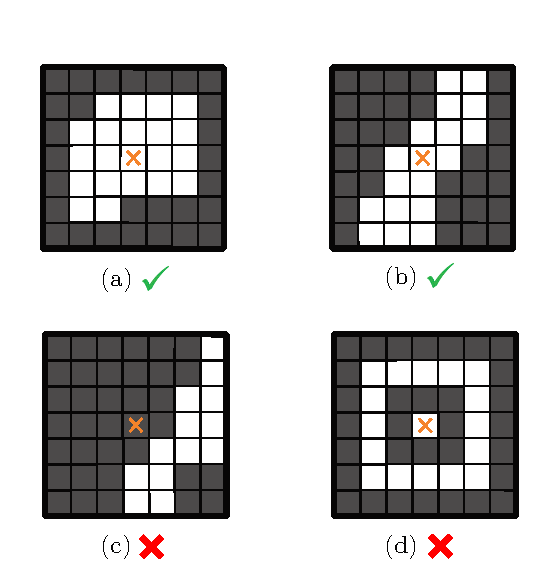
\includegraphics[width=0.99\textwidth]{./figures/LSIMasks/valid_masks.pdf} % 0.45
        \captionof{figure}[Examples of expected and not expected masks]{Examples of expected (\textbf{a-b}) and not expected (\textbf{c-d}) binary 2D \maskname masks. }
    \label{fig:valid_masks}
\end{minipage}\hfill
\begin{minipage}[t]{0.58\textwidth}
\centering
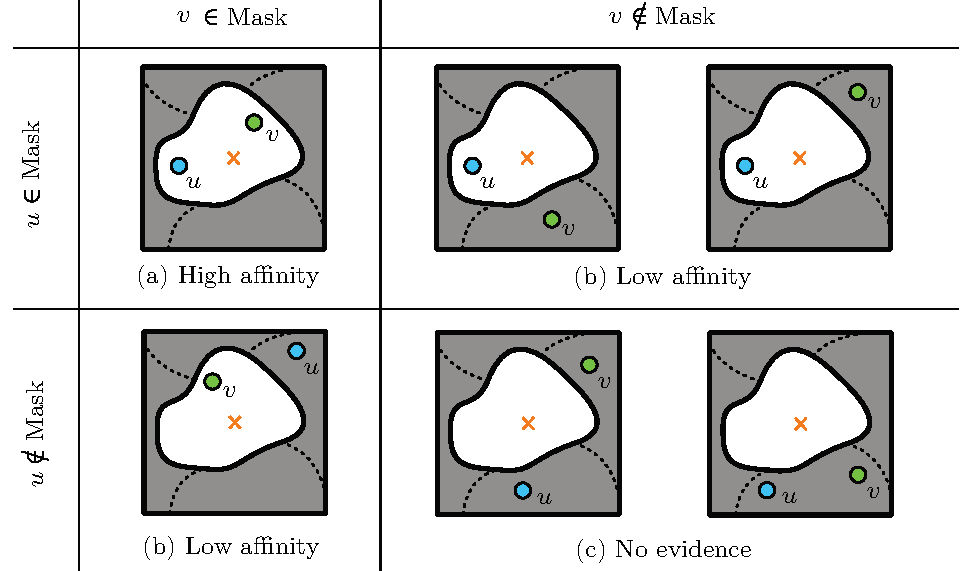
\includegraphics[width=0.99\textwidth]{./figures/LSIMasks/mask_cases_new.pdf} % 0.45
        \captionof{figure}[Affinities from single-instance masks]{Computing instance-aware affinity between pixels $u$ and $v$ from instance masks associated to the central pixel in the patch (orange cross). 
        % Dashed lines represent ground-truth boundaries separating neighboring segments. 
        % We distinguish three cases: \textbf{(a)} when both pixels are part of the mask, a high affinity between the pixels is predicted; \textbf{(b)} when only one of them is part of the mask, we predict a low affinity; \textbf{(c)} when both pixels are not part of the mask, nothing can be said about their affinity.
        }
    \label{fig:mask_cases}
\end{minipage}
\end{figure}

\subsection{Training Encoded Central Instance Masks End-To-End}\label{sec:encoding_masks}
% In this section, we briefly review the strong baseline model used in our comparison experiments that has been widely used in instance segmentation  (see \emph{\sparseBr branch} in Fig. \ref{fig:main_figure}a).
In several related work approaches \cite{liu2018affinity,Gao_2019_ICCV,lee2017superhuman,wolf2018mutex,bailoni2019generalized}, affinities between pairs of pixels are predicted for a predefined sparse stencil representing a set of $N$ short- and long-range neighborhood relations for each pixel  ($N=8$ \emph{\sparseBr branch} of Fig. \ref{fig:main_figure}a). The $N$ output feature maps  are then trained with a binary classification loss. 
% In other words, we do not predict one full \maskname mask for each pixel of the input image, but only a predefined pattern of $N$ out of $K\times K$ pixels of each \maskname mask. 
% As shown in the \emph{\sparseBr branch} of Fig. \ref{fig:main_figure}a, the backbone model is trained to output $N$ feature maps, each representing a different neighborhood relation. We then define a dense channel-wise S\o rensen-Dice loss for every pixel \cite{wolf2018mutex,dice1945measures,sorensen1948method}.
% As compared to L2 or binary cross-entropy, this loss is more robust against class imbalance.
% prediction and / or target sparsity, a desirable quality for our application in neuron segmentation, since transitions between neuron instances occupy very few pixels in a three-dimensional volume.


On paper, this training method can be easily generalized to output a feature map of size $K^2 \times H \times W$ and thus predict a full $K\times K$ \maskname mask for each pixel of the input image (see \emph{\denseBr branch} in Fig. \ref{fig:main_figure}b).
Nevertheless, in practice, this model has prohibitively large memory requirements for meaningful values of $K$, precluding application to 3D data of interest here.

However, among the $2^{K\cdot K}$ conceivable binary masks $\hat{\mathcal{M}}_{\coord{u}}: \mathcal{N}_{K^2} \rightarrow \{0,1\}$, in practice only a tiny fraction corresponds to meaningful instance masks (see some examples in Fig. \ref{fig:valid_masks}). 
This suggests that it is possible to find a compact representation that spans the manifold of expected instance shapes.

As our first main contribution, we test this assumption by training a model end-to-end to predict, for each pixel $\coord{u}\in H\times W$ of the input image, a latent vector $z_{\coord{u}}\in \mathbb{R}^Q$ encoding the $K \times K$ \maskname mask $\mathcal{M}_{\coord{u}}$ centered at pixel $\coord{u}$ (see \emph{\encBr branch} in Fig. \ref{fig:main_figure}c). 
The backbone model is first trained to output a more compact $Q\times H\times W$ feature map and
% as compared to $K^2 \times H \times W$. 
then a tiny convolutional decoder network is applied to each pixel of the feature map to decode masks.
During training, decoding one mask for each pixel in the image would be too memory consuming. Thus, we randomly sample $R$ pixels with coordinates $\coord{u}_1, \ldots, \coord{u}_R$ and only decode the associated masks $\mathcal{M}_{\coord{u}_1}, \ldots, \mathcal{M}_{\coord{u}_R}$. 
Given the ground-truth \maskname masks $\hat{\mathcal{M}}_{\coord{u}_i}$ defined in Eq. \ref{eq:target_masks}, the training loss is then defined according to the S\o rensen-Dice coefficient formulated for fuzzy set membership values, similarly to what was done in \cite{wolf2018mutex}.
% \begin{equation}
% \mathcal{J}_{\mathrm{MaskLoss}} = - \frac{\sum_{i=1}^R \sum_{\coord{n} \in \mathcal{N}_{K\times K}} \big(1-\mathcal{M}_{\coord{u}_i}(\coord{n})\big)\cdot \big(1-\hat{\mathcal{M}}_{\coord{u}_i}(\coord{n})\big)}{\sum_{i=1}^R \sum_{\coord{n}\in \mathcal{N}_{K\times K}} \Big( \big(1-\mathcal{M}_{\coord{u}_i}(\coord{n})\big)^2 + \big(1-\hat{\mathcal{M}}_{\coord{u}_i}(\coord{n})\big)^2 \Big)}.
% \end{equation} 
Ground-truth labels are not always pixel-precise and it is often impossible to estimate the correct label for pixels that are close to a ground-truth label transition. Thus, in order to avoid noise during training, we predict completely empty masks for pixels that are less than two pixels away from a label transition, so that the model is trained to predict single-pixel clusters along the ground-truth boundaries. In our experiments, this approach performed better than masking the training loss along the boundaries.


\subsection{Predicting Multi-Scale Central Instance Masks}\label{sec:multiscale_patches}
Previous related work \cite{lee2017superhuman,liu2018affinity,Gao_2019_ICCV} shows that predicting long-range affinities between distant pixels improves accuracy as compared to predicting only short-range ones. However, predicting large \maskname masks would translate to a bigger model that, on 3D data, would have to be trained on a small 3D input field of view.
This, in practice, usually decreases accuracy because of the reduced 3D context available to the network.
% whose size is an important hyper-parameter in neuron segmentation since the correct detection of mitochondria and other organelles strongly depends on how much surrounding 3D context is provided during training.
Thus, we instead predict multiple \maskname masks of the same window size $7 \times 7 \times 5$ but at different resolutions, so that the lower the resolution the larger the size of the associated patch in the input image. 
% Note that the size of \maskname masks in this work is kept fixed only for simplicity reasons.
These multiple masks at different resolutions are predicted by adding several \emph{\encBr branches} along the hierarchy of the decoder in the backbone model, which in our case is a 3D U-Net \cite{ronneberger2015u,cciccek20163d} (see Fig.~\ref{fig:model_architecture}). 
In this way, the encoded \maskname masks at higher and lower resolutions can be effectively learned at different levels in the feature pyramid of the U-Net.




% !TEX root = ../../main.tex


\begin{algorithm}[t]
  \begin{flushleft}
  \caption{Affinities from Aggregated Central Instance Masks}
   \hspace*{\algorithmicindent} \textbf{Input:} Graph $\mathcal{G}(V,E)$; \maskname masks $\mathcal{M}_{\coord{u}}: \mathcal{N}_{K\times K} \rightarrow [0,1]$  \\
  \hspace*{\algorithmicindent} \textbf{Output:} Affinities $\bar{a}_e\in[0,1]$ with variance $\sigma^2_e$ for all edges $e\in E$\\
  \hspace*{\algorithmicindent} 
  \begin{algorithmic}[1]
  \footnotesize
  % \scriptsize
  % \small
      % \State Initial clustering: $\Pi=\{\{v_1\}, \ldots, \{v_{|V|}\}\}$
      % \State Initialize interactions between clusters with $ = w^+_e - w^-_e$
      \For{each edge $e=(\coord{u}, \coord{v})\in E$ in graph $\mathcal{G}$}
        \State Get coordinates $\coord{u}=(u_x,u_y)$ and $\coord{v}=(v_x,v_y)$ of pixels linked by edge $e$
        \State Collect all $T$ masks $\mathcal{M}_{\coord{c}_1},\ldots,\mathcal{M}_{\coord{c}_T}$ including both pixel $\coord{u}$ and pixel $\coord{v}$
        \State Init. vectors $[a_1,\ldots,a_T] = [\evidW_1,\ldots,\evidW_T] = 0$ for affinities and evidence weights
        \For{$i\in 1, \ldots,T$}
            \State Get relative coords. of $\coord{u}$ and $\coord{v}$ with respect to the central pixel $\coord{c}_i$
            \State $a_i \gets \min \big(\mathcal{M}_{\coord{c}_i}(\coord{u} - \coord{c}_i), \,\mathcal{M}_{\coord{c}_i}(\coord{v} - \coord{c}_i)\big)$ \Comment{Fuzzy-AND: both values active}
            \State $\evidW_i \gets \max \big(\mathcal{M}_{\coord{c}_i}(\coord{u} - \coord{c}_i), \,\mathcal{M}_{\coord{c}_i}(\coord{v} - \coord{c}_i)\big)$ \Comment{Fuzzy-OR: at least one value active}
        \EndFor
        \State Get weighted affinity average $\bar{a}_e= \sum_{i} a_i \evidW_i\,/\,\sum_{i}\evidW_i$ 
        \State Get weighted affinity variance $\sigma^2_e = \sum_{i} \evidW_i (a_i-\bar{a}_e)^2\,/\,\sum_{i}\evidW_i$
      \EndFor
      \State
      \Return $\bar{a}_e, \sigma^2_e$ for each $e\in E$
  \end{algorithmic}
    \label{alg:computing_affinities}
  \end{flushleft}

\end{algorithm}
\begin{figure}[t]
\centering
        % \includegraphics[width=0.4\textwidth,trim=0.25in 0.25in 0.68in 0.36in,clip]{./figures/LSIMasks/SSBM_experiments.pdf} % 0.45
        \includegraphics[width=\textwidth]{./figures/LSIMasks/mask_aggregation.pdf} % 0.45
        \caption[Proposed method to average overlapping masks]{Proposed method to average overlapping masks and compute the affinity between pixel $u$ and pixel $v$ (highlighted in red in the ground-truth segmentation on the left). For simplicity, we only consider three masks among all the ones including both pixels $u$ and $v$. 
        % For each of the three masks in the lower part of the figure, we highlight in red the predicted probabilities for $u$ and $v$ to be part of the instance that covers the central pixel of the mask. 
        In \emph{Mask 1}, only $v$ is part of the mask, so there is a strong evidence for no affinity between $u$ and $v$; in \emph{Mask 2},  $u$ is predicted to be part of the mask only with a low confidence, so the contribution of this mask in the final average will be weak; in \emph{Mask 3}, both pixels are not part of the \maskname mask, so there is no evidence about their affinity. 
        The final affinity value of edge $(u,v)$ is given by the weighted average of the collected affinities $a_i$ weighted with the evidence weights $\evidW_i$: $\bar{a}_e= \sum_{i=1}^3 a_i \evidW_i\,/\,\sum_{i}\evidW_i$
        }
    \label{fig:alg_explained}
\end{figure}


% \section{Extracting Affinities from Central Instance Masks}
\section{Affinities with Uncertainty from Aggregated Masks}\label{sec:aggr_affs}
In order to obtain an instance segmentation from the predictions of the model presented in Sec. \ref{sec:model}, we now compute instance-aware pixel-pair affinities for a given sparse $N$-neighborhood structure (see Table \ref{tab:neighborhood_structures} in supplementary material for details about the structure) and use them as edge weights of a pixel grid-graph $\mathcal{G}(V,E)$, such that each node represents a pixel / voxel of the image. The graph is then partitioned to obtain object instances.
% \TODO{Section intro} Second contribution; two ways
% In this section, we propose two ways to perform something similar and use the predicted per-pixel \maskname masks to define the edge weights of a grid-graph.

In this section, we propose an algorithm that, without the need of any threshold parameter, aggregates predictions from overlapping \maskname masks and outputs edge weights with associated uncertainty.
Related work either thresholds the predicted \maskname masks \cite{januszewski2018high,hirsch2020patchperpix,meirovitch2016multi} or computes Intersection over Union (IoU) scores for overlapping patches \cite{liu2016multi}. However, an advantage of predicting pixel-pair affinities / pseudo-probabilities as compared to IoU scores is that affinities can easily be translated into attractive and repulsive interactions in the grid-graph 
% i.e. edge with either positive or negative weights, 
and a parameter-free partitioning algorithm can be employed to yield instances.
% Related work in \cite{liu2016multi} aggregate \maskname masks by computing Intersection over Union (IoU) scores for overlapping patches, however these scores cannot be translated into attractive and repulsive cues of the graph, so hierarchical agglomerative clusterings 

Here, we propose a simple algorithm to aggregate predictions from multiple patches: Fig. \ref{fig:alg_explained} shows a simplified example of how Algorithm \ref{alg:computing_affinities} computes the affinity for an edge $e$ linking a pair of pixels $\coord{u}$ and $\coord{v}$.
As a first step, the algorithm loops over all predicted \maskname masks including both $\coord{u}$ and $\coord{v}$. 
% For example, if $\coord{u}$ and $\coord{v}$ are direct neighbors and the predicted masks have shape $K\times K$, then there will be $K(K-1)$ masks including both pixel $\coord{u}$ and $\coord{v}.$\footnote{Note that here we ignore possible boundary effects by considering two pixels close to the image border.} 
However, not all these masks are informative, as we visually explain in Fig.~\ref{fig:mask_cases}: a mask $\mathcal{M}_{\coord{c}_i}$ centered at pixel $\coord{c}_i$ provides any evidence about the affinity between pixels $\coord{u}$ and $\coord{v}$ only if at least one of the two pixels belongs to the mask (fuzzy OR operator at line 8 in Alg. \ref{alg:computing_affinities}).
If both pixels do not belong to it, we cannot say anything about whether they belong to the same instance (see Fig. \ref{fig:mask_cases}c). We model this with an evidence weight $\evidW_i\in[0,1]$, which is low when both pixels do not belong to the mask.
% If both pixels do not belong to it, then the evidence weight  goes to zero (see Fig. \ref{fig:mask_cases}c).
On the other hand, when at least one of the two pixels belongs to the mask, we distinguish two cases (fuzzy AND operator at line 7 in Alg. \ref{alg:computing_affinities}): i)
both pixels belong to the mask  (case in Fig. \ref{fig:mask_cases}a), so by transitivity we conclude they should be in the same instance and their affinity $a_i$ should tend to one; 
ii) only one pixel belongs to the mask (case in Fig. \ref{fig:mask_cases}b), so that according to this mask they are in different instances and their affinity should tend to zero. 

At the end, we compute a weighted average $\bar{a}_e$ and variance $\sigma^2_e$ of the collected affinities from all overlapping masks, such that masks with more evidence will contribute more on average, and the obtained variance is a measure of how consistent were the predictions across masks. 
The algorithm was implemented on GPU using PyTorch and the variance was computed via Welford's online stable algorithm \cite{welford1962note}.






% !TEX root = ../../main.tex


\section{Experiments on Neuron Segmentation}
We evaluate and compare our method on the task of neuron segmentation in electron microscopy (EM) image volumes. This application is of key interest in connectomics, a field of neuro-science with the goal of reconstructing neural wiring diagrams spanning complete central nervous systems. 
% Currently, only proof-reading or manual tracing yields sufficient accuracy for correct circuit reconstruction \cite{schlegel2017learning}, thus further progress is required in automated reconstruction methods (see Fig. \ref{fig:MWS_segm} for an example of output neuron segmentation).
We test our method on the competitive CREMI 2016 EM Segmentation Challenge \cite{cremi} that is currently the neuron segmentation challenge with the largest amount of training data available. The dataset comes from serial section EM of \emph{Drosophila} fruit-fly brain tissue and consists of 6 volumes of $1250\times 1250\times 125$ voxels at resolution $4\times 4\times 40$ nm$^3$, three of which come with publicly available training ground truth. 
We achieved the best scores by downscaling the resolution of the EM data by a factor $(\frac{1}{2},\frac{1}{2},1)$, since this helped increasing the 3D context provided as input to the model.
We use the second half of CREMI sample C as validation set for our comparison experiments in Table \ref{tab:val_results} and then we train a final model on all the three samples with available ground truth labels to submit results to the leader-board in Tab. \ref{tab:test_results}. 
Results  are evaluated using the CREMI score, which is given by the geometric mean of Variation of Information Score (VOI split + VOI merge) and Adapted Rand-Score (Rand-Score) \cite{arganda2015crowdsourcing}. See Sec.~\ref{sec:cremi_details} for more details on data augmentation, strongly inspired by related work.




\subsection{Architecture details of the tested models}\label{sec:models_details}
As a backbone model we use a 3D U-Net consisting of a hierarchy of four feature maps with anisotropic downscaling factors $(\frac{1}{2},\frac{1}{2},1)$, similarly to \cite{lee2019learning,lee2017superhuman,wolf2018mutex}. 
% U-Net with three levels in the feauter map hierarchy, involving downscaling factors $(1, \frac{1}{2},\frac{1}{2})$
Models are trained with the Adam optimizer and a batch size equal to one. Before applying the loss, we slightly crop the predictions to prevent training on borders where not enough surrounding context is provided. 
Fig. \ref{fig:model_architecture} shows the details on the 3D-UNet architecture and Table \ref{tab:neighborhood_structures} lists the sparse neighborhood structures predicted by the \emph{\sparseBr branches}. Only the outputs at the highest resolution (given by branches SNB$_1$, ENB$_1$ and ENB$_2$) are used to compute edge weights in the pixel grid-graph. A visualization of the predicted single-instance mask latent spaces is given in Fig. \ref{fig:PCA_embeddings}.
% - Cite architecture figure Fig: we use three type of nets, we only use highest res predictions for computing affinities of the graph

The input volume has shape $272 \times 272\times12$ which is equivalent to a volume of $544\times 544\times 12$ voxels in the original resolution $4\times 4\times 40$ nm$^3$. Before to apply the loss, we crop the predictions to a shape $224\times 224\times 9$ in order to avoid border artifacts\footnote{Instead of cropping directly the final predictions, we perform several crops in the decoder part of the UNet model (see Upsample + Crop connections in Fig. \ref{fig:model_architecture}) in order to optimize GPU-memory usage.}.
The final model trained on all available ground truth labels is trained with a slightly larger input volume of $288\times 288\times 14$.

 
\paragraph{Baseline Model (SNB)} As a strong baseline, we re-implement the current state-of-the-art and train a model to predict affinities for a sparse neighborhood structure (Fig. \ref{fig:main_figure}a). We perform deep supervision by attaching three \emph{\sparseBr branches} (SNB) at different levels in the hierarchy of the UNet decoder and train the coarser feature maps to predict longer range affinities. Details about the used neighborhood structures and the architecture can be found in Table \ref{tab:neighborhood_structures} and Fig. \ref{fig:model_architecture}.

\paragraph{Proposed Model (ENB)} We then train a model to predict encoded \maskname masks (Fig. \ref{fig:main_figure}c). Similarly to the baseline model, we provide deep supervision by attaching four \emph{\encBr branches} (ENB) to the backbone U-Net. As explained in Sec. \ref{sec:multiscale_patches}, all branches predict 3D masks of shape $7 \times 7 \times 5$, but at different resolutions $(1,1,1)$, $(\frac{1}{4},\frac{1}{4},1)$ and $(\frac{1}{8},\frac{1}{8},1)$, as we show in the architecture in Fig. \ref{fig:model_architecture}. A visualization of the learned latent spaces is given in Fig. \ref{fig:PCA_embeddings}.

\paragraph{Combined Model (SNB+ENB)} Finally, we also train a combined model to predict both \maskname masks and a sparse neighborhood of affinities, by providing deep supervision both via \emph{\encBr} and \emph{\sparseBr} \emph{branches}. The backbone of this model is then trained with a total of seven branches: three branches equivalent to the ones used in the baseline model SNB, plus four additional ones like those in the ENB model (see Fig. \ref{fig:model_architecture}).  


\paragraph{Efficient Affinities for any Sparse Neighborhood}\label{sec:efficient_affs}
An advantage of training dense \maskname masks is that the graph $N$-neighborhood structure can be defined at prediction time, after the model has been trained. As an alternative to the method presented in Sec. \ref{sec:aggr_affs} that aggregates overlapping masks, here we propose the following efficient approach to predict affinities for a sparse neighborhood structure: Given a model that has been already trained end-to-end to predict encoded \maskname masks, we stack few additional convolutional layers that are trained to convert the $Q$-dimensional latent mask space to $N$ output feature maps representing affinities for the chosen sparse neighborhood structure. These last layers are not trained jointly with the full model, so in practice they are very quick and easy to train with a binary classification loss. By using this method, we avoid to decode all masks explicitly (one for each pixel) and achieve great time and memory savings.
As a result, we obtain a model that at inference time is no more memory-consuming than the current state-of-the-art approach predicting affinities only for a specific sparse neighborhood structure.

\begin{figure}[tbp]
\centering
        % \includegraphics[width=0.4\textwidth,trim=0.25in 0.25in 0.68in 0.36in,clip]{./figures/LSIMasks/SSBM_experiments.pdf} % 0.45
        \includegraphics[width=\textwidth]{./figures/LSIMasks/UNet_architecture.pdf} % 0.45
        \vspace{1em}
        \caption{\textbf{The architecture of the model}, which is strongly inspired by the 3D-UNet models proposed in \cite{lee2017superhuman,funke2018large}. 
        Red numbers indicate the number of used feature maps.
        As we explain in Sec. \ref{sec:models_details}, in this work we consider three models: i) a baseline model based on the three \emph{\sparseBr branches} SNB$_{i=1,2,3}$, shown in the figure; ii) another model based on the four \emph{\encBr branches} ENB$_{i=1,2,3,4}$; iii) and, finally, a combined model trained with all seven branches shown in the Figure.
        Even though the input of the model is a 3D volume, here, for simplicity, we show an example of 2D input image taken from the stack. As output of the \emph{\sparseBr branches} SNB$_{i=1,2,3}$, we show few channels representing some of the predicted affinities (see Table \ref{tab:neighborhood_structures} for details on the sparse neighborhood structures predicted by each branch SNB$_{i=1,2,3}$). We also show the first three principal components of the encoded masks predicted by the \emph{\encBr branches} ENB$_{i=1,2,3,4}$. All branches ENB$_{i=1,2,3,4}$ predict \maskname masks of the same window size $7 \times 7 \times 5$, but at different resolutions.}
    \label{fig:model_architecture}
\end{figure}

\begin{figure}[tbp]
\centering
        % \includegraphics[width=0.4\textwidth,trim=0.25in 0.25in 0.68in 0.36in,clip]{./figures/LSIMasks/SSBM_experiments.pdf} % 0.45
        \includegraphics[width=\textwidth,trim=1.80in 1.4in 1.8in 1.50in,clip]{./figures/LSIMasks/MWS_segm.pdf} % 0.45
        \caption{Raw data from the validation set overlaid with the final instance segmentation obtained with our method: affinities are computed by averaging overlapping masks (MaskAggr); the final segmentation is achieved by running the Mutex Watershed algorithm on the obtained graph with positive and negative edge weights. Note that the data is 3D, hence the same color could be assigned to parts of segments that appear disconnected in 2D.}
    \label{fig:MWS_segm}
\end{figure}





\begin{figure}[tbp]
\centering
        % \includegraphics[width=0.4\textwidth,trim=0.25in 0.25in 0.68in 0.36in,clip]{./figures/LSIMasks/SSBM_experiments.pdf} % 0.45
        \includegraphics[width=\textwidth]{./figures/LSIMasks/PCA_embeddings.pdf} % 0.45
        \vspace{1em}
        \caption{\textbf{Visualization of the predicted single-instance mask latent spaces} -- Each column represents a 2D image from the 3D stack (only five are shown here). \textbf{(a)} Ground-truth labels. \textbf{(b)} Raw image given as input to the model. \textbf{(c-d-e-f)} Visualization of the first three principal components of the $32$-dimensional mask latent spaces predicted by the \encBr branches ENB$_{i=1,2,3,4}$ in our model. Note how latent spaces learned at different levels of the U-Net pyramid show different feature-scales, because they encode \maskname masks at different resolutions.}
    \label{fig:PCA_embeddings}
\end{figure}



\subsection{Graph Partitioning Methods} 
Given the predicted encoded \maskname masks, we compute affinities $a_e$ either with the average aggregation method introduced in Sec. \ref{sec:aggr_affs} (\textbf{MaskAggr}) or the efficient approach described in the previous section \ref{sec:efficient_affs}. 
The result of either is a signed pixel grid-graph, i.e. a graph with positive and negative edge weights that needs to be partitioned into instances. 
The used neighborhood connectivity of the graph, which is very similar to the one used in related work \cite{wolf2018mutex,lee2017superhuman}, is given in Table \ref{tab:neighborhood_structures}. Positive and negative edge weights $w_e$ are computed by applying the additive transformation $w_e=a_e-0.5$ to the predicted affinities.




To obtain final instances, we test different partitioning algorithms.
 % that have been already applied to neuron segmentation. 
The Mutex Watershed (\textbf{MWS}) \cite{wolf2018mutex} is an efficient algorithm to partition graphs with both attractive and repulsive weights without the need for extra parameters. It can easily handle the large graphs considered here with up to $10^8$ nodes/voxels and $10^9$ edges\footnote{Among all edges given by the chosen neighborhood structure, we add only 10\% of the long-range ones, since the Mutex Watershed was shown to perform optimally in this setup \cite{bailoni2019generalized,wolf2018mutex}.}. In Fig. \ref{fig:MWS_segm}, we show the resulting instance segmentation obtained by computing affinities from \maskname masks and then running the Mutex Watershed algorithm on the obtained graph with positive and negative edge weights.


Then, we also test another graph partitioning pipeline that has often been applied to neuron segmentation because of its robustness. This method first generates a 2D super-pixel over-segmentation from the model predictions and then partitions the associated region-adjacency graph to obtain final instances. Super-pixels are computed with the following procedure: First, the predicted direct-neighbor affinities are averaged over the two isotropic directions to obtain a 2D neuron-membrane probability map; then, for each single 2D image in the stack, super-pixels are generated by running a watershed algorithm seeded at the maxima of the boundary-map distance transform (\textbf{WSDT}). Given this initial over-segmentation, a 3D region-adjacency graph is built, so that each super-pixel is represented by a node in the graph. Edge weights of this graph are computed by averaging short- and long-range affinities over the boundaries of neighboring super-pixels. 
Finally, the graph is partitioned by applying the average agglomeration algorithm proposed in \cite{bailoni2019generalized} (\textbf{GaspAvg}).

After running the graph partitioning method, we use a simple post-processing step to delete small segments on the boundaries, most of which are given by single-voxel clusters. On the neuron segmentation predictions, we deleted all regions with less than 200 voxels and used a seeded watershed algorithm to expand the bigger segments.
% GaspAverage is more robust to noise as compared to Mutex Watershed \cite{bailoni2019generalized}, but it is considerably more computationally expensive on large graphs like the ones considered here (up to $10^8$ nodes/voxels and $10^9$ edges). Thus, in our comparison on the validation set, we also... 

  








% \begin{figure}[t]
%         \centering
% \begin{minipage}[t]{0.49\textwidth}
%     \centering
%     % \scriptsize
%         \begin{tabular}[t]{l|c}
%          Method & \makecell{CREMI-Score \\(lower is better)} \\ \midrule 
% \textbf{} \textbf{Average}& \textbf{0.226}  \\
%  Sum + Constraints \cite{levinkov2017comparative} & 0.282 \\
%  Abs. Max. \cite{wolf2018mutex} & 0.322 \\
%  Max. + Constraints & 0.324 \\
%  Sum \cite{keuper2015efficient} & 0.334 \\
%  Average + Constraints & 0.563 \\
% THRESH & 1.521 \\ 
%         \end{tabular}
%     % \captionof{table}{CREMI-Scores achieved by different linkage criteria and thresholding. All methods use the affinity predictions from our CNN as input. Scores are averaged over the three CREMI training datasets.}
%     \label{tab:results_cremi_train}
% \end{minipage}\hfill
% % \begin{minipage}[t]{0.35\textwidth}
% % \centering
% %     \scriptsize
% %     \vspace*{-1.5em}
% % \begin{tabular}[t]{l|cc}
% %         \multirow{2}{*}{Method}    & AP  & AP 50\% \\ 
% %          & \multicolumn{2}{c}{(higher is better)} \\ \midrule
% %            Panoptic-DeepLab \cite{cheng2019panopticdeeplab} & 34.6 & 57.3 \\
% %            UPSNet \cite{xiong2019upsnet} $\dagger$ & 33.0 & 59.6 \\
% %            SSAP \cite{Gao_2019_ICCV} & 32.7 & 51.8 \\
% %            AdaptIS \cite{sofiiuk2019adaptis} & 32.5 & 52.5 \\
% %            PANet \cite{liu2018path} $\dagger$ & 31.8 & 57.1 \\
% %            \textbf{GMIS Model \cite{liu2018affinity} +  Average} & \textbf{28.3} & \textbf{47.0} \\ 
% %            JOSECB \cite{neven2019instance} & 27.7 & 50.9 \\
% %            \textbf{GMIS} \cite{liu2018affinity} & \textbf{27.3} & \textbf{45.6} \\
% %            Mask R-CNN \cite{he2017mask} $\dagger$ & 26.2 & 49.9 \\
% %            SGN \cite{liu2017sgn} & 25.0 & 44.9 \\
% %            % DIN \cite{arnab2017pixelwise} & 20.0 & 38.8 \\
% %            % DWT \cite{bai2017deep} & 19.4 & 35.3 \\
% %            % InstanceCut \cite{kirillov2017instancecut} & 13.0 & 27.9 \\
% %         \end{tabular}
% %     % \caption{CityScapes \emph{test} set}
% %     % \vspace*{0.6em}
% %     \captionof{table}{Results on CityScapes test. Methods marked with~$\dagger$ are \emph{proposal-based}. Only methods that do not use external training data (such as MS COCO) are shown.}\label{tab:results_cityscapes}
% %     \label{tab:results_cityscapes_test}
% % \end{minipage}
% \end{figure}


\begin{figure}[t]
\begin{subfigure}[t]{0.32\linewidth}
\centering
\includegraphics[width=0.99\linewidth,trim=0in 0in 0in 0.2in,clip]{./figures/LSIMasks/aff_compare_designer/raw.pdf} % 
% \caption{\centering}
\end{subfigure}
\begin{subfigure}[t]{0.32\linewidth}
\centering
\includegraphics[width=0.99\linewidth,trim=0in 0in 0in 0.2in,clip]{./figures/LSIMasks/aff_compare_designer/GT.pdf} % ,clip
% \caption{\centering}
\end{subfigure}
\begin{subfigure}[t]{0.32\linewidth}
\centering
\includegraphics[width=0.99\linewidth,trim=0in 0in 0in 0.2in,clip]{./figures/LSIMasks/aff_compare_designer/dice_2.pdf} % ,clip
% \caption{\centering}
\end{subfigure}\vspace{1em}

\begin{subfigure}[t]{0.32\linewidth}
\centering
\includegraphics[width=0.99\linewidth,trim=0in 0in 0in 0.2in,clip]{./figures/LSIMasks/aff_compare_designer/dice_1.pdf} % ,clip
% \caption{\centering}
\end{subfigure}
\begin{subfigure}[t]{0.32\linewidth}
\centering
\includegraphics[width=0.99\linewidth,trim=0in 0in 0in 0.2in,clip]{./figures/LSIMasks/aff_compare_designer/mask_2.pdf} % ,clip
% \caption{\centering}
\end{subfigure}
\begin{subfigure}[t]{0.32\linewidth}
\centering
\includegraphics[width=0.99\linewidth,trim=0in 0in 0in 0.2in,clip]{./figures/LSIMasks/aff_compare_designer/mask_1.pdf} % ,trim=0.25in 0.25in 0.65in 0.36in,clip
% \caption{\centering}
\end{subfigure}


% \begin{subfigure}[t]{0.32\linewidth}
% \centering
% \includegraphics[width=0.99\linewidth,trim=0in 0in 0in 0.2in,clip]{./figures/LSIMasks/aff_compare_designer/raw.pdf} % 
% % \caption{\centering}
% \end{subfigure}
% \begin{subfigure}[t]{0.16\linewidth}
% \centering
% \includegraphics[width=0.99\linewidth,trim=0in 0in 0in 0.2in,clip]{./figures/LSIMasks/aff_compare_designer/GT.pdf} % ,clip
% % \caption{\centering}
% \end{subfigure}
% \begin{subfigure}[t]{0.16\linewidth}
% \centering
% \includegraphics[width=0.99\linewidth,trim=0in 0in 0in 0.2in,clip]{./figures/LSIMasks/aff_compare_designer/dice_2.pdf} % ,clip
% % \caption{\centering}
% \end{subfigure}
% \begin{subfigure}[t]{0.16\linewidth}
% \centering
% \includegraphics[width=0.99\linewidth,trim=0in 0in 0in 0.2in,clip]{./figures/LSIMasks/aff_compare_designer/dice_1.pdf} % ,clip
% % \caption{\centering}
% \end{subfigure}
% \begin{subfigure}[t]{0.16\linewidth}
% \centering
% \includegraphics[width=0.99\linewidth,trim=0in 0in 0in 0.2in,clip]{./figures/LSIMasks/aff_compare_designer/mask_2.pdf} % ,clip
% % \caption{\centering}
% \end{subfigure}
% \begin{subfigure}[t]{0.16\linewidth}
% \centering
% \includegraphics[width=0.99\linewidth,trim=0in 0in 0in 0.2in,clip]{./figures/LSIMasks/aff_compare_designer/mask_1.pdf} % ,trim=0.25in 0.25in 0.65in 0.36in,clip
% % \caption{\centering}
% \end{subfigure}



\caption{Comparison between different affinities and their robustness to noise. \textbf{\mbox{(a-b)}} Raw data and ground-truth labels. \textbf{(c-d)} Affinities predicted by the \emph{sparse-neighborhood branch}, which is trained with a dense binary classification loss (high affinities are red). \textbf{(e-f)} Affinities computed by averaging overlapping masks as explained in Sec. \ref{sec:aggr_affs} (MaskAggr). Affinities from averaged masks are smoother and present a more consistent boundary evidence in the noisy region highlighted by the red circle in (a). Here we show affinities along the horizontal (-4, 0, 0) and vertical (0, -4, 0) directions.}\label{fig:affs_comparison}
\end{figure}

\subsection{Results and Discussion}

\paragraph{Pre-Training of the Encoded Space} The proposed model based on an \emph{\encBr branch} can be properly trained only if the dimension $Q$ of the latent space is large enough to accommodate all possible occurring neighborhood patterns. 
To find a small but sufficiently large $Q$, we trained a convolutional Variational Auto-encoder (VAE) \cite{kingma2013auto,rezende2014stochastic} to compress binary ground-truth \maskname masks $\hat{\mathcal{M}}_{\coord{u}}$ into latent variables $z_{\coord{u}}\in \mathbb{R}^Q$ and evaluated the quality of the reconstructed binary masks via the reconstruction loss. We concluded that $Q=32$ is large enough to compress the masks considered here consisting of $7\times 7 \times 5=245$ pixels. 
As a first experiment, we tried to make use of this VAE-pretrained latent space to train the proposed \emph{\encBr branch} and predict encoded masks directly in this space by using an L2 loss on the encoded vectors. However, similarly to the findings of \cite{hirsch2020patchperpix}, this approach performed worse than directly training the full model end-to-end as described in Sec. \ref{sec:encoding_masks}. 
% \begin{itemize}
% \item Mention how we tested the latent space dimension by training a VAE (or AE) to compress binary ground-truth \maskname masks: \emph{We then test this assumption by compressing binary ground-truth \maskname masks $\hat{\mathcal{M}}_{\coord{u}}$ to latent variables $z_{\coord{u}}\in \mathbb{R}^Q$ by training a convolutional Variational Auto-encoder (VAE) \cite{kingma2013auto,rezende2014stochastic} consisting of an encoder $p_{\phi}(z_{\coord{u}}|\hat{\mathcal{M}}_{\coord{u}})$ and a decoder $p_{\phi}(\hat{\mathcal{M}}_{\coord{u}}|z_{\coord{u}})$.
% In our experiments, we evaluate how the dimension $Q$ of the latent space impacts the quality of the reconstructed binary masks and find in this way an optimal latent space dimension that is compact enough but at the same time preserves most of the information contained in the binary masks.}
% \item Mention that we also tried to pre-train the encoded space with a VAE, but this did not work better than directly training the space end-to-end (similarly to PatchPerPix). 
% \emph{In this case, we first train a VAE to encode ground-truth binary masks as explained above in Sec. \ref{sec:encoding_masks}. 
% The main backbone model is then trained to predict, for each pixel $\coord{u}$, the mean and the standard deviation of the encoded distribution $p_{\phi}(z_{\coord{u}}|\hat{\mathcal{M}}_{\coord{u}})$ predicted by the pre-trained encoder, where $\hat{\mathcal{M}}_{\coord{u}}$ is the ground truth \maskname mask associated to pixel $\coord{u}$. An L2 loss is used to pull the two encoded vectors close to each other's. 
% The reasoning behind this approach is to train the backbone model to predict the masks in a meaningful compressed latent space. 
% Nevertheless, as we will show in our experiments, this method was the least successful among the tested ones (\emph{similarly to the findings of \cite{hirsch2020patchperpix}}).}
% \end{itemize}



\paragraph{Training Encoded Masks} As we show in our validation experiments in Tab. \ref{tab:val_results}, models trained to predict encoded \maskname masks (ENB) achieved better scores than the current state-of-the-art method predicting affinities for a sparse neighborhood structure (SNB). 
% Predicting only affinities for a sparse-neighborhood, like the SBN model, is an easier task as compared to predicting large and dense neighborhood structures. 
Our interpretation of this result is that using the encoding process to predict \maskname masks encourages the model to predict segment shapes that are consistent in a larger neighborhood, which can be helpful to correctly segment the most difficult regions of the data. 
% Thus, we argue that the combined model is less likely to result in a basic boundary detector based on simple local features and it is instead more likely to learn more complex features and use for example prior information about the shape of the segments.
 % like in the models ENB and ENB+SBN, is a more challenging task than predicting affinities for a sparse-neighborhood, like for the SBN model. Thus, we argue that the models predicting \maskname masks are 
 % and instead are encouraged to learn long-range features that can be helpful in the most challenging cases.
% Moreover, ... 
% Not only improves affinities, but also the opposite. 



\paragraph{Aggregating Overlapping Masks}
In our validation experiments of Tab. \ref{tab:val_results}, we also test the affinities computed by averaging over overlapping masks (MaskAggr), as described in Sec. \ref{sec:aggr_affs}. We then partition the resulting signed graph by using the Mutex Watershed, which has empirical linearithmic complexity in the number of edges. 
Our experiments show that, for the first time on this type of more challenging neuron segmentation data, the Mutex Watershed (MWS) achieves better scores than the super-pixel-based methods (WSDT+GaspAvg), which have so far been known to be more robust to noise but also require the user to tune more hyper-parameters.   

We also note that the MWS achieves competitive scores only with affinities computed from aggregating overlapping masks (MaskAggr).
This shows that the MWS algorithm can take full advantage of the \maskname aggregation process by assigning the highest priority to the edges with largest attractive and repulsive weights that were consistently predicted across overlapping masks.

On the other hand, most of the affinities trained with the \emph{\sparseBr} \linebreak \emph{branch} and a dense binary classification loss are almost binary, i.e. they present values either really close to zero or really close one (see comparison between different types of affinities in Fig. \ref{fig:affs_comparison}).
% In Fig. \ref{fig:affs_comparison} we compare affinities predicted either by averaging \maskname masks or by directly predicting them as a binary classification output of the model trained with a dense channel-wise S\o rensen-Dice loss. 
%\footnote{In practice, this effect is even stronger when the binary classification loss is based on the S\o rensen-Dice coefficient like the one used here.}.
This is not an ideal setup for the MWS, which is a greedy algorithm merging and constraining clusters according to the most attractive and repulsive weights in the graph.
In fact, in this setting the MWS can often lead to over-segmentation and under-segmentation artifacts like those observed in the output segmentations of the (SNB+ENB+MWS) and (SNB+MWS) models. Common causes of these mistakes can be for example inconsistent predictions from the model and partially missing boundary evidence, which are very common in this type of challenging application (see Fig. \ref{fig:affs_comparison} for an example). 
% On the other hand, 
% Thus, we first note that these affinities are substantially different from those computed by averaging over overlapping masks as described in Sec. \ref{sec:aggr_affs} \TODO{Fig?}.
 % This fact is also shown in Table \ref{tab:val_results} by the validation scores achieved by the Mutex Watershed.

Finally, we also note that superpixel-based methods did not perform equally well on affinities computed from aggregated masks and the reason is that these methods were particularly tailored to perform well with the more \emph{binary-like} classification output of the \emph{\sparseBr branch}.



% \begin{table}[t]
% \centering
% \scriptsize
% \begin{minipage}[t]{\textwidth}
%     \centering
%         \begin{tabular}[t]{L{18em} c M{8.7em} c}
%         Model & \makecell{Partitioning\\algorithm} & \makecell{CREMI-Score \\(lower is better)} & \makecell{No superpixels\\ required}  \\ \midrule
% GaspUNet+SNB+EffAff \cite{bailoni2019generalized} & WSDT+LMC  &  0.221 & \HollowBox \\
% PNIUNet+SNB+EffAff \cite{lee2017superhuman} & Z-Watershed+Agglo  & 0.228 & \HollowBox \\
% GaspUNet+SNB+EffAff \cite{bailoni2019generalized} & GaspAvg & 0.241 & \CrossedBox \\
% \textbf{OurUNet+ENB+SNB+MaskAggr} &\textbf{MWS} & \textbf{0.246} & \CrossedBox \\
% OurUNet+ENB+EffAff& WSDT+GaspAvg  & 0.268 & \HollowBox \\
% MALAUNet+EffAff \cite{funke2018large} & WSDT+Multicut  & 0.276 & \HollowBox \\
% OurUNet+ENB+SNB+EffAff & WSDT+GaspAvg & 0.280 & \HollowBox \\
% CRUNet \cite{zeng2017deepem3d} & 3D-Watershed & 0.566  & \HollowBox \\
% LFC+EffAff \cite{parag2017anisotropic} & Z-Watershed+Agglo & 0.616  & \HollowBox \\
%         \end{tabular}
%         \vspace*{0.99em}
%     \caption{Representative excerpt of the published methods currently part of the CREMI leaderboard \cite{cremiChallenge} (March 2020). The best method proposed in this work (highlighted in bold) achieves competitive scores and is based on an efficient parameter-free algorithm that does not rely on superpixels.}
%     \label{tab:test_results}
% \end{minipage}
% \end{table}


\begin{table}[t]
% \tiny
\centering
\scriptsize
\rowcolors{2}{white}{gray!25} % \rowcolors{<starting row index>}{<dispari row color>}{<pari row color>}
  % {\renewcommand{\arraystretch}{1.3}
  % \resizebox{\textwidth}{!}{
        \begin{tabular}[t]{c c c c c c c}
         % Method & \makecell{CREMI-Score \\(lower is better)} \\ \midrule 
\makecell{Train \\ Sparse \\Neighbor.\\(SNB)} & \makecell{Train\\ Encoded\\Masks\\(ENB)} & \makecell{Aggregate\\Overlapping\\Masks \\(MaskAggr)} & \makecell{Partitioning \\algorithm} &\makecell{No\\superpixels\\required}  & \makecell{CREMI-Score \\(lower is better)} & \makecell{VI-merge \\(lower is better)} \\ \toprule 

\CrossedBox & \CrossedBox & \CrossedBox & MWS & \CrossedBox & \textbf{0.153} & 0.272 \\
% \CrossedBox & \HollowBox & \textbf{0.153} & \textbf{0.272} \\
% ENB+SNB+MaskAggr} & \textbf{MWS} & \textbf{0.153} & \textbf{0.272} \\
\HollowBox & \CrossedBox & \CrossedBox & MWS & \CrossedBox & 0.184 & 0.273 \\
\HollowBox & \CrossedBox & \HollowBox & MWS & \CrossedBox & 0.419 & 0.302 \\
\CrossedBox & \CrossedBox & \HollowBox & MWS & \CrossedBox & 0.532 & 0.447 \\
\CrossedBox & \HollowBox & \HollowBox & MWS & \CrossedBox & 1.155 & 0.874 \\ \midrule
\HollowBox & \CrossedBox & \HollowBox & WSDT+GaspAvg & \HollowBox & 0.173 & \textbf{0.234} \\
\CrossedBox & \CrossedBox & \HollowBox & WSDT+GaspAvg & \HollowBox & 0.237 & 0.331 \\
\CrossedBox & \HollowBox & \HollowBox & WSDT+GaspAvg & \HollowBox & 0.254 & 0.355 \\
\CrossedBox & \CrossedBox & \CrossedBox & WSDT+GaspAvg & \HollowBox& 0.334 & 0.388 \\
\HollowBox & \CrossedBox & \CrossedBox & WSDT+GaspAvg & \HollowBox & 0.357 & 0.391 \\

% ENB+SNB & MutexWatershed & _affs &  &  &  & 0.585 & 0.257 & 0.454 & 0.878 \\
% SNB & MutexWatershed & _affs &  &  &  & 0.910 & 0.344 & 0.671 & 1.736 \\
% SNB & MutexWatershed & _affs_withLR &  &  &  & 1.126 & 0.487 & 0.766 & 1.837 \\
% ENB & WSDT+MC & 0.178 & 0.040 & 0.233 & 0.557 \\
% ENB+SNB & WSDT+MC & 0.241 & 0.082 & 0.331 & 0.377 \\
% SNB & WSDT+MC & 0.257 & 0.087 & 0.355 & 0.399 \\
% ENB+SNB+MaskAggr & MutexWatershed & _affs &  &  &  & 0.269 & 0.086 & 0.370 & 0.470 \\
% ENB+MaskAggr & MutexWatershed & _affs &  &  &  & 0.302 & 0.095 & 0.365 & 0.595 \\
% ENB+SNB & MutexWatershed & _affs_withLR &  &  &  & 0.416 & 0.145 & 0.385 & 0.803 \\


% % % & & SNB & 1.144 & 0.875 \\ 
% % & & SNB+ENB & \textbf{0.115} & 0.222 \\
% % & & SNB & 0.119 & \textbf{0.219} \\
% % GaspAverage  & & SNB+ENB+MaskAggr &  0.156 & 0.277 \\
% % & &ENB & 0.173 & 0.242 \\
% % & &ENB+MaskAggr & 0.188 & 0.281 \\ \midrule
% & &SNB+ENB & \textbf{0.130} & \textbf{0.234} \\
% WSDT+GaspAverage & & SNB & 0.147 & 0.258 \\
% && ENB & 0.173 & 0.240 \\ \midrule
% & &SNB+ENB & \textbf{0.135} & \textbf{0.235} \\
% WSDT+MC & & SNB &  0.151 & 0.258 \\
% & & ENB & 0.178 & 0.240 \\ \midrule
% & & SNB+ENB+MaskAggr & \textbf{0.155} & 0.278 \\
% & & ENB+MaskAggr & 0.183 & \textbf{0.275} \\
% MutexWatershed & & ENB & 0.417 & 0.311 \\
% & & SNB+ENB &  0.531 & 0.449 \\
% % & & SNB+ENB & 0.539 & 0.376 \\
% & & SNB & 0.895 & 0.634 \\ 
% % Superpixels without long-range:
% % UNet+SNB+ENB & WSDT+GASP-Avg & 0.137 & 0.260 \\
% % UNet+SNB & WSDT+GASP-Avg & 0.188 & 0.333 \\
% % UNet+ENB & WSDT+GASP-Avg & 0.197 & 0.299 \\
% % Multicut without long range:
% % UNet+SNB+ENB & WSDT+MC & 0.127 & 0.245 \\
% % UNet+ENB & WSDT+MC & 0.156 & 0.248 \\
% % UNet+SNB & WSDT+MC & 0.183 & 0.317 \\
% % Superpixels ong MaskAggr
% % UNet+SNB+ENB+MaskAggr & WSDT+GASP-Avg-LR & 0.219 & 0.309 \\
% % UNet+SNB+ENB+MaskAggr & WSDT+GASP-Avg & 0.229 & 0.316 \\
% % UNet+ENB+MaskAggr & WSDT+GASP-Avg-LR & 0.243 & 0.316 \\
% % UNet+ENB+MaskAggr & WSDT+GASP-Avg & 0.248 & 0.323 \\


        \end{tabular}
        % }
        \vspace{1em}
        \caption{Comparison experiments on our CREMI validation set. Training encoded \maskname masks (ENB) achieved better scores than the current state-of-the-art approach training only affinities for a sparse neighborhood (SNB). The model that performed best was the one using the method proposed in Sec. \ref{sec:aggr_affs} to average overlapping masks (MaskAggr). } \label{tab:val_results}
\end{table}



\paragraph{Training Both Masks and a Sparse Neighborhood} In our validation experiments, the combined model, which was trained to predict both a sparse neighborhood (SNB) and encoded \maskname masks (ENB), achieved the best scores and yielded sharper and more accurate mask predictions.
In general, providing losses for multiple tasks simultaneously has often been proven beneficial in a supervised learning setting.
Moreover, the dense gradient of the \emph{\encBr branch}, which focuses on locally correct predictions, nicely complements the sparse gradient\footnote{The gradient of the \emph{\encBr branch} is sparse, due to GPU-memory constraints as explained in Sec. \ref{sec:encoding_masks}.} of the \emph{\encBr branch}, which focuses on predictions that are consistent in a larger neighborhood. We expect this to be another reason why the combination of affinities and \maskname masks performed best in our experiments. 
% In our case, the better performances of the combined model could also be explained by the fact that, due to GPU-memory restrictions, the \emph{\encBr branch} was trained only with a sparse gradient from a small fraction of all the predicted encoded masks (see Sec. \ref{sec:encoding_masks}), whereas the \emph{\sparseBr branch} received gradient for every pixel in the output feature map. \\
% On the other hand, the combined model ENB+SNB, which receives dense gradient from the \emph{\sparseBr branch}, predicted sharper and more accurate \maskname mask as compared to the ENB model. Thus, to summarize, our results show that the combined model trained to predict both affinities and \maskname masks performs better than the models trained to solve the two tasks singularly, which is a common behavior often observed in supervised learning. \\





\paragraph{Results on Test Samples} The evaluation on the three test samples presented in Tab. \ref{tab:test_results} confirms our findings from the validation experiments: among the methods tested here, the best scores are achieved by the combined model (ENB+SNB) and by using the Mutex Watershed algorithm (MWS) on affinities averaged over overlapping masks (MaskAggr).
Our method achieves comparable scores to the only other method in the leader-board that does not rely on super-pixels (line 3 in Table \ref{tab:test_results}). This method uses the average agglomeration algorithm GaspAvg proposed in \cite{bailoni2019generalized} instead of the MWS. GaspAvg has been shown to be more robust to noise than Mutex Watershed, however it is also considerably more computationally expensive to run on large graphs like the ones considered here. 

% The other leading entries in the leaderboard are all given by methods that are very similar to our baseline model SNB, which in our validation experiments consistently performed worse.
% A possible explanation of this result could be that all our trained models seem to suffer particularly from the \emph{glia-confusion problem}, that has been already observed in related work on neuron segmentation \TODO{\cite{lee2019learning,januszewski2018high}}. Glia (putative astrocyte) are segments that look quite different from other neurons and are usually considered separately in the final reconstructed diagram of neural circuit connectivity. They often present a main body with a lot of very thin processes that can be \emph{self-touching}. 
% % glia segments are substantially different from the other neurons and are usually considered separately in the final reconstructed diagram of neural circuit connectivity. Glia segments usually present a main body with a lot of very thin glial processes
% Locally, at these self-touching points, glial thin fragments look like distinct segments with clear membrane evidence separating them, even though in the full 3D volume they are connected and hence share the same ground truth label.
% When this happens during training, the model is initially confused and then usually tries to ``memorize'' these self-touching examples by predicting high affinity values despite the clear membrane evidence.
% % When these self-touching examples happen on the training set, despite the clear neuron membrane evidence, the model is trained to predict the same 
% % Every time there is a glia fragment in the training dataset presents two narrow processes that are self-touching, the model is trained to predict one single label for them, even though these processes locally appear like two distinct neurons with clear membrane evidence separating them.
% In practice, this can often lead to wrong merge decisions on the validation and test set, because the model confuses distinct narrow neurons for self-touching fragments of the same glia and wrongly predicts a high merge-affinity connecting them.
% In future work, we plan to process this type of glial fragments differently, similarly to related work \TODO{\cite{lee2019learning,januszewski2018high}}. 

\begin{table}[t]
\centering
\scriptsize
\rowcolors{2}{white}{gray!25} % \rowcolors{<starting row index>}{<dispari row color>}{<pari row color>}
\begin{minipage}[t]{\textwidth}
    \centering
        \begin{tabular}[t]{l c c c c c c}
        Model & \makecell{Train \\ Sparse \\Neighbor.\\(SNB)} & \makecell{Train\\ Encoded\\Masks\\(ENB)} & \makecell{Aggregate\\Overlapping\\Masks \\(MaskAggr)} & \makecell{Partitioning\\algorithm} & \makecell{No\\superpixels\\ required}  & \makecell{CREMI-Score \\(lower is better)}  \\ \midrule
GaspUNet\cite{bailoni2019generalized} & \CrossedBox & \HollowBox & \HollowBox & WSDT+LMulticut & \HollowBox & \textbf{0.221} \\
GaspUNet\cite{bailoni2019generalized} & \CrossedBox & \HollowBox & \HollowBox & GaspAvg & \CrossedBox & 0.224  \\
PNIUNet\cite{lee2017superhuman} & \CrossedBox & \HollowBox & \HollowBox & Z-Watershed+Agglo & \HollowBox & 0.228 \\
\textbf{OurUNet} & \CrossedBox & \CrossedBox & \CrossedBox &MWS & \CrossedBox & 0.246  \\
\textbf{OurUNet} & \HollowBox & \CrossedBox & \HollowBox &  WSDT+GaspAvg  & \HollowBox & 0.268  \\
MALAUNet\cite{funke2018large} & \CrossedBox & \HollowBox & \HollowBox & WSDT+Multicut & \HollowBox & 0.276  \\
\textbf{OurUNet} & \CrossedBox & \CrossedBox & \HollowBox & WSDT+GaspAvg & \HollowBox & 0.280  \\
CRUNet\cite{zeng2017deepem3d} & \HollowBox & \HollowBox & \HollowBox & 3D-Watershed & \HollowBox & 0.566   \\
LFC\cite{parag2017anisotropic} & \CrossedBox & \HollowBox & \HollowBox & Z-Watershed+Agglo & \HollowBox & 0.616  \\
        \end{tabular}
        \vspace*{0.99em}
    \caption{Representative excerpt of the published methods currently part of the CREMI leaderboard \cite{cremi}. The best method proposed here achieves competitive scores and is based on an efficient parameter-free algorithm that does not rely on superpixels. For more details about the partitioning algorithms used by related work, see references in the first column.}
    \label{tab:test_results}
\end{minipage}
\end{table}

\begin{table}[tp]
\small
\centering
\footnotesize
\rowcolors{2}{white}{gray!25} % \rowcolors{<starting row index>}{<dispari row color>}{<pari row color>}
  % {\renewcommand{\arraystretch}{1.3}
  % \resizebox{\textwidth}{!}{
        \begin{tabular}[t]{M{10em} M{8em} M{8em} M{8em} }
         % Method & \makecell{CREMI-Score \\(lower is better)} \\ \midrule 
\thead{Graph neighborhood\\structure\\(16 neighbors)} & \thead{SNB$_1$\\(18 neighbors)} &  \thead{SNB$_2$\\(10 neighbors)}  & \thead{SNB$_3$\\(10 neighbors)} \\ \toprule 
(0, 0, -1)      & (0, 0, -1)    & (0, 0, -1)    & (0, 0, -1) \\
(-1, 0, 0)      & (-1, 0, 0)    & (-4, 0, 0)    & (-4, 0, 0) \\
(0, -1, 0)     & (0, -1, 0)     & (0, -4, 0)    & (0, -4, 0) \\
(-4, 0, 0)     & (-4, 0, 0)     & (0, 0, -2)    & (0, 0, -2) \\
(0, -4, 0)     & (0, -4, 0)     & (0, 0, -3)    & (0, 0, -3) \\
(-4, -4, 0)    & (-4, -4, 0)    & (0, 0, -4)    & (0, 0, -4) \\
(4, -4, 0)     & (4, -4, 0)     & (-14, 0, 0)   & (-12, 0, 0) \\
(-4, 0, -1)     & (-4, 0, -1)   & (0, -14, 0)   & (0, -12, 0) \\
(0, -4, -1)     & (0, -4, -1)   & (-14, -14, 0) & (-12, -12, 0) \\
(-4, -4, -1)    & (-4, -4, -1)  & (14, -14, 0)  & (12, -12, 0) \\
(4, -4, -1)     & (4, -4, -1)   &  - & - \\
(0, 0, -2)      & (0, 0, -2)    & - & - \\
(-8, -8, 0)    & (0, 0, -3)     & - & - \\
(8, -8, 0)     & (0, 0, -4)     & - & - \\
(-12, 0, 0)    & (-8, -8, 0)    & - & - \\
(0, -12, 0)    & (8, -8, 0)     & - & - \\
-                & (-12, 0, 0)   & - & - \\
-               & (0, -12, 0)   & - & - \\
        \end{tabular}
        % }
        \vspace{3em}
        \caption{\textbf{Sparse neighborhood structures} --  
        In this table, we represent sparse neighborhood structures (see for example the one shown in Fig. \ref{fig:main_figure}a) as lists of offsets $(\delta_x,\delta_y, \delta_z)$ indicating the relative coordinates of neighboring pixels with respect to the central pixel.
        The first column shows the neighborhood structure of the pixel grid-graph, such that each pixel / node is connected to 16 neighbors. In the following columns, we provide the neighborhood structures predicted by the three \emph{\sparseBr branches} SNB$_i$ used in our model (see architecture in Fig. \ref{fig:model_architecture}).
        These neighborhood structures were inspired by the ones used in \cite{wolf2018mutex,lee2017superhuman} but were adapted to our version of the CREMI data that is downscaled by a factor $(\frac{1}{2},\frac{1}{2},1)$. Note that the offsets provided here are given in the downscaled resolution.} \label{tab:neighborhood_structures}
\end{table}





% !TEX root = ../../main.tex

\section{Conclusions}
We have presented a new proposal-free method predicting encoded \maskname masks in a sliding window style, one for each pixel of the input image, and introduced a parameter-free approach to aggregate predictions from overlapping masks and obtain all instances concurrently.
When applied to large volumetric biological images, the resulting method proved to be strongly robust to noise and compared favorably to competing methods that need super-pixels and hence more hyper parameters.
The proposed method also endows its predictions with an uncertainty measure, depending on the consensus of the overlapping  \maskname masks. In future work, we plan to use these uncertainty measures to estimate the confidence of individual instances, which could help facilitate the subsequent proof-reading step still needed in neuron segmentation.




% Conclusions and final stuff
%!TEX root = ../main.tex


\chapter*{Conclusions}
\addcontentsline{toc}{chapter}{Conclusions} 
In this thesis, we have developed new graph-based instance segmentation methods and applied them to the task of automated segmentation of large neural tissue 3D image volumes. Previous methods often relied on multi-step post-processing pipelines based on superpixels, which usually required the user to spend time tuning task-dependent hyper-parameters. 
On the other hand, the simple graph partitioning algorithms presented in this thesis are parameter-free. Some of them, when combined with informative edge weights from a deep neural network, achieve state-of-the-art accuracies on two neuron segmentation challenges.

In Chapter ~\ref{chapter:MWS}, we have introduced a new efficient algorithm, the Mutex Watershed, for the clustering of graphs with both attractive and repulsive edge weights. The proposed algorithm has low computational complexity and is closely related to the Kruskal's algorithm for minimum spanning tree computation \cite{kruskal1956shortest}.
We prove that this algorithm finds the global optimum of an objective function, and that this objective is closely related to the multicut optimization problem as well as the power watershed framework.
The Mutex Watershed algorithm achieved state-of-the-art results on the ISBI neuron segmentation challenge, and, after our results were published, it also became part of other two state-of-the-art segmentation pipelines used for neuron segmentation \cite{hirsch2020patchperpix,lee2019learning}.

In Chapter \ref{chapter:GASP}, we have then proved that the Mutex Watershed algorithm is part of a larger generalized framework, named GASP, for agglomerative clustering of graphs with both positive and negative edge weights. We have analyzed several theoretical and empirical properties of the algorithms in it, by exploring new and existing combinations of linkage criteria and applying them to different types of graphs. Algorithms based on an average linkage criterion proved to be simple and robust approaches when applied to an instance segmentation task. On large volume images, these simple average agglomeration algorithms achieved state-of-the-art results on the competitive CREMI neuron segmentation challenge. 

Finally, in Chapter \ref{chapter:LSI}, we introduced a novel proposal-free method predicting encoded single-instance masks in a sliding window style, one for each pixel of the input image, and introduced a parameter-free approach to aggregate predictions from overlapping masks and obtain all instances concurrently. The resulting pipeline proved to be strongly robust to noise when applied to large neuron segmentation volumetric images. 
The method also endows its predictions with an uncertainty measure, depending on the consensus of the overlapping  single-instance masks. Future work could use these uncertainty measures to estimate the confidence of individual instances, which may help to facilitate the subsequent proof-reading step still needed in neuron segmentation.

The proposed unifying framework for agglomerative clustering algorithms also opens several opportunities for further research. Future work could investigate which objectives are optimized by the algorithms included in the GASP framework, and study how they relate to the multicut / correlation clustering problem. A generalized GASP objective function could also be linked to existing cost functions for hierarchical clustering on unsigned graphs with positive edge weights \cite{moseley2017approximation,cohen2019hierarchical,dasgupta2016cost}. 
Another research direction is the structured learning of graph edge weights, which optimizes the segmentation performance directly. The fact that this approach has already been successfully applied to instance segmentation and other graph partitioning algorithms \cite{funke2018large,kong2018recurrentPix,wolf2017learned,cerrone2019end} suggests that it could be similarly used to achieve an end-to-end training of the segmentation pipelines presented in this thesis that rely on agglomerative algorithms in the GASP framework.


\begin{appendices}
% !TEX root = ../../main.tex

\chapter{GASP}
\section{Implementation and complexity of GASP} \label{sec:detailed_impl}
\subsection{Update rules}
During the agglomerative process, the interaction between adjacent clusters has to be properly updated and recomputed, as shown in Algorithm \ref{main_alg}.  
An efficient way of implementing these updates can be achieved by representing the agglomeration as a sequence of \emph{edge contractions} in the graph. Given a graph $\mathcal{G}(V,E,\cost)$ and a clustering $\Pi$, we define the associated \emph{contracted graph} $\tilde{\mathcal{G}}_\Pi(\tilde{V}, \tilde{E}, \tilde{\cost})$, such that there exists exactly one representative node $|\tilde{V} \cap S| = 1$ for every cluster $S \in \Pi$ . Edges in $\tilde{E}$ represent adjacency-relationships between clusters 
and the signed edge weights $\tilde{\cost}_e$ are given by inter-cluster interactions $\tilde{\cost}(e_{uv})=\interact_{S_u,S_v}$, where $S_u$ denotes the clustering including node $u$. 
For the linkage criteria tested in this article, when two clusters $S_u$ and $S_v$ are merged, the interactions between the new cluster $S_u \cup S_v$ and each of its neighbors depend only on the previous interactions involving $S_u$ and $S_v$. Thus, we can recompute these interactions by using an \emph{update rule} $f$ that does not involve any loop over the edges of the original graph $\mathcal{G}$:
\begin{align}
  \interact(S_u \cup S_v,S_t) =& f\Big[ \interact(S_u,S_t), \interact(S_v,S_t) \Big] \\
  =& f(\tilde{\cost}(e_{ut}), \tilde{\cost}(e_{vt})) 
\end{align}
In Fig. \ref{fig:edge_contraction_and_contr_graph} we show an example of edge contraction and in Table \ref{tab:linkage_criteria_explicit} we list the update rules associated to the linkage criteria we introduced in Table \ref{tab:linkage-criteria}.

\afterpage{ %
  \begin{algorithm*}[p]
    \caption{Implementation of \algname{} - Phase 1}
  \hspace*{\algorithmicindent} \textbf{Input:} $\mathcal{G}(V,E,w^+,w^-)$ with $N$ nodes and $M$ edges; boolean \texttt{{\color{blue}addCannotLinkConstraints}} \\
  \hspace*{\algorithmicindent} \textbf{Output:} Final clustering \\
    \hspace*{\algorithmicindent} 
    \begin{algorithmic}[1]
        \State $\tilde{\mathcal{G}}(\tilde{V},\tilde{E}) \gets \mathcal{G}(V,E,w^+,w^-)$  \Comment{Init. contracted graph}
        \State \texttt{UF} $\gets$ initUnionFind($V$) \Comment{Init. data structure representing clustering}
          \State PQ.push$(|w_e|, e) \quad \forall e \in E $  \Comment{Init. priority queue in desc. order of $|w_e|=|w_e^+ - w_e^-|$, $\mathcal{O}(|E|)$}
          \State \texttt{canBeMerged}$[e] \gets$ \texttt{True} $\,\,\, \forall e\in E$ \Comment{Init. cannot-link constraints}
      \State
        \While{PQ is \textbf{not} empty}
          \State $\tilde{w}, e_{uv} \gets $ PQ.popHighest() \Comment{$\mathcal{O}(\log |E|)$}
          \State \textbf{assert} \texttt{UF}.find($u$) $\neq$ \texttt{UF}.find($v$) \Comment{Edges in PQ always link nodes in different clusters}
          \If{({\color{green}\textbf{$\tilde{w} > 0$}}) \textbf{and} \texttt{canBeMerged}$[e_{uv}]$}
            \State PQ, \texttt{canBeMerged}, $\tilde{E}$ $\gets$ \textsc{UpdateNeighbors}($u,v$)
            \State $\tilde{V} \gets \tilde{V} \setminus \{ v\}$, $\quad \tilde{E} \gets \tilde{E} \setminus \{ e_{uv}\}$ \Comment{Update contracted graph}
            \State \texttt{UF}.merge($u,v$) \Comment{Merge clusters, $\mathcal{O}(\alpha(|E|))$}
          \ElsIf{({\color{red}\textbf{$\tilde{\cost} \leq 0$}}) \textbf{and} {\color{blue}\texttt{addCannotLinkConstraints}}}
            \State \texttt{canBeMerged}$[e_{uv}] \gets$ \texttt{False} \Comment{Constrain the two clusters}
          \EndIf
        \EndWhile
        \State
        \Return Final clustering given by union-find data structure  \texttt{UF}
    \end{algorithmic}
    \hspace*{1.5cm} 
      \begin{algorithmic}[1]
      \Function{UpdateNeighbors}{$u,v$}
        \State $\mathcal{N}_u = \{ t \in \tilde{V} | e_{ut}\in \tilde{E}  \}$
        \State $\mathcal{N}_v = \{ t \in \tilde{V} | e_{vt}\in \tilde{E}  \}$ 
        \For{$t \in \mathcal{N}_v$ } \Comment{Loop over neighbors in $\tilde{\mathcal{G}}$ of deleted node $v$}
          \State $\tilde{E} \gets \tilde{E} \setminus \{e_{vt}\}$
          \State $\tilde{w}_{vt} \gets$ PQ.delete($e_{vt}$) \Comment{Delete edge $e_{vt}$ from PQ and get the old edge weight, $\mathcal{O}(\log |E|)$}
          \State \texttt{canBeMerged}$[e_{ut}] \gets$ \texttt{canBeMerged}$[e_{ut}]$ \textbf{and} \texttt{canBeMerged}$[e_{vt}]$
          \If{$t \in \mathcal{N}_u$ }\Comment{Check if $t$ is a common neighbor of $u$ and $v$}
            \State $\tilde{w}_{ut} \gets$ PQ.delete($e_{ut}$)  \Comment{$\mathcal{O}(\log |E|)$}
            \State PQ.push($ |f(\tilde{w}_{ut}, \tilde{w}_{vt})|, e_{ut}$) \Comment{$\mathcal{O}(\log |E|)$  }
          \Else
            \State $\tilde{E} \gets \tilde{E} \cup \{e_{ut}\}$
            \State PQ.push($ |\tilde{w}_{vt}|, e_{ut}$) \Comment{$\mathcal{O}(\log |E|)$}
          \EndIf
        \EndFor
        \State
        \Return PQ, \texttt{canBeMerged}, $\tilde{E}$
      \EndFunction
    \end{algorithmic}
    \label{detailed_alg}
  \end{algorithm*}
  % \begin{figure*}[t]
  %         \centering
  %         \includegraphics[width=0.7\textwidth]{./figures/GASP/proof_abs_max_example.pdf} % left bottom right top
  % \caption{\algname{} with \emph{AbsMax} linkage: Example representing the only case of edge contraction $e_{uv}$ that would introduce a positive attractive interaction between two constrained clusters. Note this can actually never happen with an \emph{AbsMax} linkage, because edge $e_{ut}$ has a lower absolute priority as compared to $e_{uv}$, so clusters $u$ and $t$ cannot have been constrained before $u$ and $v$ are merged. \TODO{Remove?}
  % }
  % \label{fig:abs_max_proof_example}  
  % \end{figure*}
  \begin{algorithm*}[p]
    \caption[Alternative formulation of the Mutex Watershed Algorithm]{Mutex Watershed Algorithm proposed in Chapter \ref{chapter:MWS}}
  \hspace*{\algorithmicindent} \textbf{Input:} $\mathcal{G}(V,E,w^+,w^-)$ with $N$ nodes and $M$ edges \\
  \hspace*{\algorithmicindent} \textbf{Output:} Final clustering \\
    \hspace*{\algorithmicindent} 
    \begin{algorithmic}[1]
        \State \texttt{UF} $\gets$ initUnionFind($V$) 
        \For{$(u,v)=e\in E$ in descending order of $|w_e|=|w_e^+ - w_e^-|$}
          \If{\texttt{UF}.find($u$) $\neq$ \texttt{UF}.find($v$)} \Comment{Check if $u,v$ are already in the same cluster}
            \If{({\color{green}\textbf{$w_e > 0$}}) \textbf{and} \texttt{canBeMerged}($u,v$)}  \Comment{Check for cannot-link constraints}
              \State \texttt{UF}.merge($u,v$) and inherit constraints of parent clusters
            \ElsIf{({\color{red}\textbf{$w_e \leq 0$}})}
              \State Add cannot-link constraints between parent clusters of $u,v$
            \EndIf
          \EndIf
        \EndFor
        \State
        \Return Final clustering given by union-find data structure \texttt{UF}
    \end{algorithmic}
    \label{alg:mutex_watershed}
  \end{algorithm*}
  \clearpage
}

\subsection{Implementation} 
Our implementation of \algname{} is based on an union-find data structure and a heap allowing deletion of its elements. 
In Phases 2 and 3, \algname{} is equivalent to a standard hierarchical agglomerative clustering algorithm with complexity $\mathcal{O}(N^2 \log N)$. In Algorithm \ref{detailed_alg}, we show our implementation of phase 1, involving cannot-link constraints.
In phase 1, the algorithm starts with each node assigned to its own cluster and sorts all edges $e\in E$ in a heap/priority queue (PQ) by their absolute weight $|\cost_e|=|w_e^+ - w_e^-|$ in descending order, so that the most attractive and the most repulsive interactions are processed first. It then iteratively pops one edge $e_{uv}$ from PQ and, depending on the priority $\tilde{\cost}_{uv}$, does the following: in case of attractive interaction $\tilde{\cost}_{uv}>0$, provided that $e_{uv}$ was not flagged as a cannot-link constraint, merge the connected clusters, perform an edge contraction of $e_{uv}$ in $\tilde{\mathcal{G}}_\Pi$ and update the priorities of new double edges as explained in Fig. \ref{fig:edge_contraction_and_contr_graph}. 
If, on the other hand, the interaction is repulsive ($\tilde{\cost}_{uv}\leq 0$) and the option \texttt{addCannotLinkContraints} of Alg. \ref{detailed_alg} is \texttt{True}, then the edge $e_{uv}$ is flagged as cannot-link constraint.


\begin{table}[t]
\centering
    \small
    % \vspace{-2em}
\begin{tabular}[t]{r | l }
            \toprule
            Linkage criteria & Update rule $f$ \\        
            \midrule
            Sum: & \thead[l]{$f(\tilde{\cost}_1,\tilde{\cost}_2) = \tilde{\cost}_1+\tilde{\cost}_2$} \\ 
            \makecell[r]{Absolute \\Maximum:} & \thead[l]{
            $
            f(\tilde{\cost}_1,\tilde{\cost}_2) = \begin{cases} 
            \tilde{\cost}_1 & \text{if}\,\, |\tilde{\cost}_1|>|\tilde{\cost}_2|\\
            \tilde{\cost}_2 & \text{otherwise}
             \end{cases} 
            $}
               \\ 
            \makecell[r]{Average:} & \thead[l]{$f(\tilde{\cost}_1,\tilde{\cost}_2) = \mathrm{weightAvg}\{ \tilde{\cost}_1, \tilde{\cost}_2 \} $}                 \\ 
            Single: & \thead[l]{$f(\tilde{\cost}_1,\tilde{\cost}_2) = \max \{ \tilde{\cost}_1, \tilde{\cost}_2 \}  $} \\
            Complete:& \thead[l]{$f(\tilde{\cost}_1,\tilde{\cost}_2) = \min \{ \tilde{\cost}_1, \tilde{\cost}_2 \}  $} 
        \end{tabular}\vspace{1em}
        \caption[Update rules associated to different linkage criteria]{The table lists the update rules $f(\tilde{\cost}_1, \tilde{\cost}_2)$ associated to the linkage criteria of Table \ref{tab:linkage-criteria} and that are used to efficiently update the interactions between clusters.}
\label{tab:linkage_criteria_explicit}  
\end{table}
\begin{figure}[t]
        \centering
        \includegraphics[width=0.48\textwidth]{./figures/GASP/edge_contraction.pdf} % left bottom right top
    \centering
    \caption[Example of edge contraction]{Example of edge contraction. First row: original graph $\mathcal{G}$; clustering $\Pi$ (gray shaded areas) with dashed edges on cut; cannot-link constraints (violet bars). Second row: contracted graph $\tilde{\mathcal{G}}_\Pi$. In step ii), edge $e_{uv}$ is contracted and node $v$ deleted from $\tilde{\mathcal{G}}_\Pi$. In step iii), double edges $e_{tu}$ and $e_{tv}$ resulting from the edge contraction are replaced by a single edge with updated interaction.}\label{fig:edge_contraction_and_contr_graph}  
\end{figure}



\subsection{Complexity} 
In the main loop of Phase 1, the algorithm iterates over all edges, but the only iterations presenting a complexity different from $\mathcal{O}(1)$ are the ones involving a merge of two clusters, which are at most $N-1$. By using a union-find data structure (with path compression and union by rank) the time complexity of \texttt{merge}$(u, v)$ and \texttt{find}($u$) operations is $\mathcal{O}(\alpha(N))$, where $\alpha$ is the slowly growing inverse Ackerman function. The algorithm then iterates over the neighbors of the merged cluster (at most $N$) and updates/deletes values in the priority queue ($\mathcal{O}(\log |E|)$). 
Therefore, 
similarly to a heap-based implementation of hierarchical agglomerative clustering, our implementation of \algname{} - Phase 1 has a complexity of $\mathcal{O}(N^2 \log N)$. In the worst case, when the graph is dense and $|E|=N^2$, the algorithm requires $\mathcal{O}(N^2)$ memory. Nevertheless, in our practical applications the graph is much sparser, so $\mathcal{O}(|E|)=\mathcal{O}(N)$. 
With a single-linkage, corresponding to the choice of the \emph{Maximum} update rule in our framework, the algorithm can be implemented by using the more efficient Kruskal's Minimum Spanning Tree algorithm with complexity $\mathcal{O}(N \log N)$, but only when cannotLinkConstraints are not used. 
Moreover, \algname{} with \emph{Absolute Maximum} linkage can be implemented more efficiently (see next section). %\TODO{Empirical complexity plot?}




\section{Proofs of Propositions in Section \ref{sec:alg_update_rules}}
\label{sec:proposition_proofs}

\begin{lemma} \label{lemma:absMax_and_complete_not_positive}
If \algname{} Algorithm \ref{main_alg} with \textbf{Complete linkage criteria} enforces a constraint between two clusters in \emph{Phase 1}, then the interaction between the clusters will never become positive over the course of the following agglomeration steps.
\end{lemma}
\begin{proof}
Two clusters are constrained in \emph{Phase 1} only if their interaction is repulsive and, with complete linkage,  the signed interaction between two clusters can only decrease over the course of the agglomeration. Thus, if two clusters are constrained by the algorithm, their negative interaction cannot increase and become positive later on in the agglomeration process.
\end{proof}

\begin{lemma} \label{lemma:absMax_and_complete_not_positive}
If \algname{} Algorithm \ref{main_alg} with \textbf{AbsMax linkage criteria} enforces a constraint between two clusters in \emph{Phase 1}, then the interaction between the clusters will never become positive over the course of the following agglomeration steps.
\end{lemma}
\begin{proof}
During the agglomeration the interaction between two clusters can only increase in absolute value. Thus, the negative interaction $\interact{}(S_i,S_j)<0$ between two constrained clusters can possibly become positive over the course of next agglomeration steps only if there is at least another pair of clusters in the graph that has a positive interaction $\interact{}(S_l,S_t)>0$ higher in absolute value: $|\interact{}(S_l,S_t)| > |\interact{}(S_i,S_j)|$.
If such clusters $S_l, S_t$ with positive interaction exist, we note that they must also be constrained (in the opposite case, the algorithm would have already merged them before to constrain $S_i$ and $S_j$, because their priority is higher). In other words, a constrained negative interaction can become positive only if there is already another positive constrained interaction: but this can never be the case because initially all constrained interactions are negative.
\end{proof}

\begin{lemma} \label{lemma:absMax_and_complete_property}
In the \algname{} Algorithm \ref{main_alg} with AbsMax or Complete linkage criteria (see linkage definition in Table \ref{tab:linkage-criteria}), the same final clustering is returned whether or not cannot-link constraints are enforced.
\end{lemma}
\begin{proof}
In phase 1 of Algorithm \ref{detailed_alg}, two clusters are merged only if the condition at line 9 is satisfied (i.e. when an interaction is both positive and not constrained). From Lemma \ref{lemma:absMax_and_complete_not_positive} and Lemma \ref{lemma:absMax_and_complete_not_positive} follows that with Complete and AbsMax linkage an interaction can never be both positive and constrained at the same time, so we directly conclude that the constrained and unconstrained versions of the algorithm will perform precisely the same agglomeration steps in phase 1.
In phase 2 (after constraints have been removed) no clusters are merged because all interactions are already negative (whether they previously constrained or not). Thus, both constrained and unconstrained versions of \algname{} return the same clustering $\Pi^*$.
\end{proof}

% We now prove Proposition \ref{prop:absmax_mutex}:

\absmaxmutex*

% \begin{prop} \label{prop:equiv_MWS}
% The Mutex Watershed Algorithm \ref{alg:mutex_watershed} (MWS) with empirical \linebreak $\mathcal{O}(N \log N)$ complexity introduced by \cite{wolf2018mutex} returns the same final clustering given by the \algname{} Algorithm \ref{detailed_alg} with the use of cannot-link constraints and an Absolute Maximum update rule:
% \begin{equation}\label{eq:def_abs_max}
% f_{\mathrm{Abs.Max.}}(\tilde{\cost}_1,\tilde{\cost}_2) = \begin{cases} 
%             \tilde{\cost}_1 & \text{if}\,\, |\tilde{\cost}_1|>|\tilde{\cost}_2|\\
%             \tilde{\cost}_2 & \text{otherwise}
%              \end{cases} 
% \end{equation}
% \end{prop}

% \paragraph{Remark on graph notation in \cite{wolf2018mutex}} The definition of a graph proposed by \cite{wolf2018mutex} makes a distinction between a set of positive edges $E^+$, associated with a set $W^+$ of positive scalar attributes representing merge affinities, and a set of negative edges $E^-$, associated with a set $W^-$ of positive attributes representing split tendencies. On the other hand, in our definition $\mathcal{G}(V,E,w^+,w^-)$ each edge have both an attractive $w_e^+$ and a repulsive $w_e^-$ attribute, so we can make them equivalent by defining:
% \begin{align}
% E^+ =&\,\, \{ e \in E \,\,\text{s.t.} \,\,w_e = w_e^+ - w_e^- > 0\}, \\
% E^- =&\,\, \{ e \in E \,\,\text{s.t.}\,\, w_e = w_e^+ - w_e^- \leq 0\}, \\
% W^+ =&\,\, \{ |w_e| \,\,\text{s.t.}\,\, e \in E^+\},\\
%  W^- =&\,\, \{ |w_e| \,\,\text{s.t.}\,\, e \in E^-\}.
% \end{align}


\begin{proof}%[Proof of Proposition \ref{prop:absmax_mutex}]
From Lemma~\ref{lemma:absMax_and_complete_property} it directly follows that \algname{} with AbsMax linkage criterion returns the same final clustering whether or not cannot-link constraints are enforced. In the following, we prove that MWS (see pseudocode \ref{alg:mutex_watershed}) and the constrained AbsMax version of \algname{} also return the same clustering.
Both algorithms sort edges in descending order of the absolute interactions $|w_e|$ and then iterate over all of them. The only difference is that MWS, after merging two clusters, does not update the interactions between the new cluster and its neighbors. 
However, since with an Abs. Max. linkage the interaction between clusters is simply given by the edge with highest absolute weight $|w_e|$, the order by which edges are iterated over in \algname{} is never updated. Thus, both algorithms perform precisely the same steps and return the same clustering.
% Next, we prove that \algname{} with AbsMax linkage method returns the same final clustering whether or not cannot-link constraints are enforced. In the \algname{} Algorithm \ref{detailed_alg}, the interactions between clusters are updated only when two clusters are merged and the condition at line 9 is satisfied (an interaction is both positive and not constrained). 
% We also observe that, in the unconstrained version of \algname{}, the predicate \texttt{canBeMerged} at line 9 can never be false because cannot-link constraints are never introduced at line 14. \TODO{Rephrase}
% Let us now contradict the initial hypothesis and assume by absurd that the constrained version of \algname{} introduces a cannot-link constraints between two clusters sharing a positive interaction $\tilde{w}>0$ and outputs a different clustering as compared to the unconstrained version. 
% This can happen only in the situation shown in Fig. \ref{fig:abs_max_proof_example}, when two clusters $u$ and $v$ are merged together and share a common neighboring node $t$ having the following two properties: a) $u$ and $t$ are already constrained and share a repulsive interaction $w_{ut}\leq0$, b) $v$ and $t$ share an attractive interaction $w_{vt}>0$ that is higher in absolute value $|w_{vt}|>|w_{ut}|$. 
% Then, according to Eq. \ref{eq:def_abs_max}, \TODO{} the new merged cluster $uv$ and $t$ are constrained and share a positive interaction. 
% But this case can never happen, since if $|w_{vt}|>|w_{ut}|$ then clusters $v$ and $t$ are merged before clusters $u$ and $t$ are constrained.  
\end{proof}
% \begin{prop} \label{prop:abs_max_cannot_link_property}
% The \algname{} Algorithm \ref{detailed_alg} with the Absolute Maximum linkage defined in Eq. \ref{eq:def_abs_max} returns the same final clustering whether or not cannot-link constraints are enforced. 
% \end{prop}
% \begin{proof}
% \end{proof}

% \subsubsection{Weight-shift invariance of \algname{} algorithms}
\begin{figure}[tp]
% \begin{subfigure}[t]{0.48\textwidth}
\centering
\includegraphics[width=0.8\textwidth,trim=0in 0in 0in 0in,clip]{./figures/GASP/counter-examples/counter-example-GAEC.pdf}
% \caption{Original graph and dendrogram}
% \end{subfigure}

% \vspace{2em}
% \begin{subfigure}[t]{0.48\textwidth}
% \centering
% \includegraphics[width=\textwidth,trim=0in 0in 0in 0in,clip]{./figures/GASP/counter-examples/counter-example-GAEC-shifted.pdf}
% \caption{Graph with shifted edge-weights ($\alpha=-3$) and GAEC dendrogram}
% \end{subfigure}
        \caption[Counter-example: GAEC is not weight-shift invariant]{ Counter-example showing that GAEC is not weight-shift invariant.
        } \label{fig:counter_examples_shift_inv_GAEC}
\end{figure}
\begin{figure}[tp]
% \begin{subfigure}[t]{0.48\textwidth}
\centering
\includegraphics[width=0.8\textwidth,trim=0in 0in 0in 0in,clip]{./figures/GASP/counter-examples/counter-example.pdf}
% \caption{Original graph and dendrogram}
% \end{subfigure}

% \vspace{2em}
% \begin{subfigure}[t]{0.48\textwidth}
% \centering
% \includegraphics[width=\textwidth,trim=0in 0in 0in 0in,clip]{./figures/GASP/counter-examples/counter-example-shifted.pdf}
% \caption{Graph with shifted edge-weights ($\alpha=+2$) and dendrogram}
% \end{subfigure}
        \caption[Counter-examples for not weight-shift invariant algorithms]{ Counter-example showing that HCC-Sum, MWS, HCC-Avg, and HCC-Single are not weight-shift invariant.
        } \label{fig:counter_examples_shift_inv}
\end{figure}

\invariantAlgs*
\begin{proof}
Theorem 1 in \cite{chehreghani2020hierarchical} proves that hierarchical clustering with Average (HC-Avg), Single (HC-Single), and Complete linkage (HC-Complete) are weight-shift invariant.

The same is not true for \algname{} with Sum linkage criteria (GAEC and HCC-Sum), because by adding a constant $\alpha$ to all edge weights $w_e$, the interaction between two clusters $S_i$ and $S_j$ is increased by a factor $\alpha |E_{ij}|$, which depends on the number of edges  $|E_{ij}|$ connecting the two clusters. Thus, when all edge weighs of the graph are shifted, the agglomeration order may change. For a simple example of this, it is enough to consider the toy graph in Fig.~\ref{fig:intro_figure}a and shift the weights of the graph by $\alpha=-3$ (see Fig.~\ref{fig:counter_examples_shift_inv_GAEC}).


The constrained versions of \algname{} (HCC-Avg and HCC-Single) are also not weight-shift invariant: here, the algorithm merges or constrains clusters in a given order, depending on the absolute interactions $|\interact{}(S_i, S_j)|$ between clusters; so, when edge weights are shifted by a constant $\alpha$, the sorting by absolute value can change arbitrarily together with the agglomeration order, as we show in the counter-example of Fig.~\ref{fig:counter_examples_shift_inv}.
Similarly, the Mutex Watershed algorithm is not weight-shift invariant because it uses a linkage criterion that compares weights by their absolute values (see again counter-example in Fig.~\ref{fig:counter_examples_shift_inv}.
\end{proof}

% \subsubsection{Ultrametrics defined by \algname{}} 



\begin{restatable}{prop}{firstUltraMetricProperty}
\label{prop:ultraMetric1}
Consider a graph $\mathcal{G}(V,E,w_e)$, a linkage criterion $\interact{}$, and an agglomerative algorithm returning a binary rooted tree $T$ with height $h_T$. Then, $(V, d_{T})$ defined in Eq.~\ref{eq:UM_def} is an ultrametric if and only if the following is true:
 % iff the interaction $\interact{}_{T}(u, v)$ associated to the least common ancestor ${(u\vee v)\in T}$ is both lower than the interaction of any other $(u\vee v)$-descendant node and higher than the interaction of any other $(u\vee v)$-ancestor node in the tree $T$. In formulae, this is equivalent to saying that, $\forall u,v,t \in V$:
\begin{gather}
\forall u,v,t \in V \nonumber \\
 h_T(u, v) < h_T(u, t) \Rightarrow \interact{}_{T}(u,v) \geq \interact{}_{T}(u,t) \label{eq:UM_assumption}
 % h_T(u, v) < h_T(u, t) \Leftrightarrow \interact{}_{T}(u,v) > \interact{}_{T}(u,t). 
\end{gather}
In words, condition \ref{eq:UM_assumption} means: if the algorithm merges nodes $u,v$ before to merge nodes $u,t$, then the signed interaction $\interact{}_{T}(u,v)$ between $u$ and $v$ has to be higher or equal than $\interact{}_{T}(u,t)$.
% In words, $(V, d_{T})$ is an ultrametric iff the interaction $\interact{}_{T}(u, v)$ associated to the least common ancestor ${(u\vee v)\in T}$ is both lower than any other $(u\vee v)$-descendant node and higher than any other $(u\vee v)$-ancestor node in the tree $T$.
\end{restatable}
\begin{proof}
% Let us first analyze assumption \ref{eq:UM_assumption}. From $(\Rightarrow)$, we have that:
% \begin{equation}\label{eq:assumption_side_1}
% h_T(u \vee v) < h_T(u \vee t) \Rightarrow \interact{}_{T}(u,v) > \interact{}_{T}(u,t). 
% \end{equation}
% In words, if the algorithm first merges node $v$ together with node $u$ and later on merges node $t$ with node $u$, then the signed interaction $\interact{}_{T}(u,v)$ between $u$ and $v$ has to be stronger than $\interact{}_{T}(u,t)$. On the other hand, the $(\Leftarrow)$ side of Eq.~\ref{eq:UM_assumption} can be rewritten as:
% \begin{equation}\label{eq:assumption_side_2}
% h_T(u \vee v) \geq h_T(u \vee t) \Rightarrow \interact{}_{T}(u,v) \leq \interact{}_{T}(u,t).
% \end{equation}
% % which in words means: if node $t$ was merged with $u$ at the same or at an earlier iteration  together with node $u$ and later on merges node $t$ with node $u$, then the interaction $\interact{}_{T}(u,v)$

From the definition of $d_{T}$, it follows that:
\begin{align}
d_{T}(u,u) &= 0 \qquad &\forall u\in V \label{eq:dist_1} \\ 
d_{T}(u,v) &\geq 0 \qquad &\forall u,v \in V \label{eq:dist_2}\\
d_{T}(u,v)& =d_{T}(v,u) \qquad &\forall u,v \in V. \label{eq:dist_3}
\end{align}
 % $d_{T}(u,v)=d_{T}(v,u)$, $d_{T}(u,u)= 0$, and $d_{T}(u,v)\geq 0$ for each $u,v \in V$.
In order to show that $(V, d_{T})$ is an ultrametric, we only need to prove the ultrametric property:
\begin{equation}\label{eq:UM_property_original}
d_T(u,v) \leq \max \{d_T(u,t), d_T(v,t)\} \quad \forall u,v,t \in V.
\end{equation}
When at least two of the three nodes $u,v,t \in V$ are the same, this property follows from Eq.~\ref{eq:dist_1} and Eq.~\ref{eq:dist_2}. When nodes $u,v,t\in V$ are distinct, from the definition of $d_{T}$ it follows that Eq.~\ref{eq:UM_property_original} is equivalent to:
\begin{equation}\label{eq:UM_property}
\interact{}_{T}(u,v) \geq \min \{\interact{}_{T}(u,t), \interact{}_{T}(v,t)\}.
\end{equation}
In the following, we prove both sides of the \emph{if and only if} statement in the proposition. First, we prove the $(\Leftarrow)$ side, i.e. that if assumption \ref{eq:UM_assumption} holds, then $(V, d_{T})$ is an ultrametric and \ref{eq:UM_property} holds. 

Case 1: in Eq.~\ref{eq:UM_property}, $t\in V$ is part of the sub-tree ${T[u \vee v]}$. In other words, the algorithm first merges node $t$ with either node $u$ or $v$, and then $u$ and $v$ are merged together. Let us assume that $t$ is first merged with $u$ (the following proof also holds for the opposite case in which $t$ is first merged with $v$):
\begin{equation}\label{eq:case_1}
h_T(u, t) < h_T(u, v) = h_T(v, t).
\end{equation}
Thus, by combining the last equation with assumption (\ref{eq:UM_assumption}), it follows that
\begin{equation}
\interact{}_{T}(u, t) \geq \interact{}_{T}(v, t) \quad  \text{and} \quad \interact{}_{T}(u, v) = \interact{}_{T}(v, t)
\end{equation}
and Eq.~\ref{eq:UM_property} follows (becoming an equality in this case).

Case 2: in Eq.~\ref{eq:UM_property}, $t\in V$ is \emph{not} part of the sub-tree ${T[u \vee v]}$. Thus, the algorithm first merges nodes $u$ and $v$, and then it merges node $t$ together with the cluster containing $u$ and $v$:
\begin{equation}
h_T(u, v) < h_T(u, t) = h_T(v, t).
\end{equation}
Thus, from assumption \ref{eq:UM_assumption} we have that
\begin{equation}
\interact{}_{T}(u, v) \geq \interact{}_{T}(u, t) \quad  \text{and} \quad \interact{}_{T}(u, v) \geq \interact{}_{T}(v, t),
\end{equation}
so also in this case Eq.~\ref{eq:UM_property} follows.
% for every distinct $u,v,t\in V$. In other words, given two leaves nodes $u,v\in V$, the depth $\interact{}_{T}(u,v)$ associated to their least common ancestor $i\in T$ should be both lower than the depth of any $i$-descendant node in $T$ and higher than any $i$-ancestor node in $T$:
%  % that have the most positive interaction   two clusters merged by the algorithm will always have an interaction that is more negative as compared to all clusters already merged and more positive than all clusters that will be merged at later iterations of the algorithm.
% \begin{equation}
% \interact{}_{T}(u,v) \geq \interact{}_{T}(u,t) \Leftrightarrow T[u \vee t] \subseteq T[u \vee v] 
% \end{equation}
%  This happens only if, at every iteration, Algorithm \ref{main_alg} merges pairs of clusters with lower and lower interactions, which is true for only certain choices of linkage criteria. %In the next section \ref{sec:alg_update_rules}, we will show that this happens only for certain linkages and only when constraints are not enforced

Next, we are left to prove the $(\Rightarrow)$ side of the \emph{if and only if} statement: if $(V, d_{T})$ is an ultrametric, then assumption \ref{eq:UM_assumption} holds.
To prove this statement, we first rephrase it in the following equivalent form: if assumption \ref{eq:UM_assumption} does not hold, then $(V, d_{T})$ is not an ultrametric and \ref{eq:UM_property} does not hold. If we negate assumption \ref{eq:UM_assumption}, there must be at least three $u,v,t \in V$ such that: 
\begin{equation}
h_T(u, v) < h_T(u, t) \quad \text{and} \quad  \interact{}_{T}(u,v) < \interact{}_{T}(u,t).
\end{equation}
The first condition, in words, is again assuming that the algorithm first merges nodes $u$ and $v$, and later it also merges node $t$ with the cluster containing $u$ and $v$. Thus, we can rephrase this assumption as:
\begin{equation}
\interact{}_{T}(u, v) < \interact{}_{T}(u, t) = \interact{}_{T}(v, t).
\end{equation}
From this, it follows that
\begin{equation}
\interact{}_{T}(u, v) < \min \{\interact{}_{T}(u, t), \interact{}_{T}(v, t)\},
\end{equation}
which is exactly the negation of the ultrametric property \ref{eq:UM_property}.
\end{proof}

\secondUltraMetricProperty*
\begin{proof}
Thanks to Prop.~\ref{prop:ultraMetric1}, we know that $(V, d_{T^*})$ is an ultrametric if and only if assumption \ref{eq:UM_assumption} holds. Thus, in the following, we will prove which variations of the \algname{} Algorithm \ref{main_alg} satisfy assumption \ref{eq:UM_assumption}. 
In other words, we need to prove in which cases \algname{} merges clusters according to a monotonously decreasing order of signed interactions $\interact{}$.

\algname{} puts clusters in a priority queue (Algorithm \ref{main_alg}, lines 5 and 15) and merges them starting from those with the highest interaction (lines 9, 19, and 26). However, the priority queue is updated each time two clusters are merged (lines 10, 20, and 27). Thus, to ensure a monotonously decreasing merging order, updated interactions involving a merged cluster should always be lower or equal than previously existing interactions (\textbf{condition 1}):
\begin{align}\label{eq:condition1}
& \forall S_i \in \Pi \setminus \{S_1, S_2\}, \nonumber \\
\interact{}(S_1 \cup S_2, S_i) &\leq \max \{ \interact{}(S_1, S_i), \interact{}(S_2, S_i)\} 
\end{align}
where $\Pi$ is a clustering, $\interact{}$ is a linkage criteria, and $S_1,S_2\in \Pi$ are two clusters merged by the algorithm at a given iteration. If this condition is true then, in the following iterations, \algname{} can only merge clusters with lower (or equal) interaction values. 

We also note that, in phase 1, the algorithm skips interactions that are both positive and constraint (condition at line 8 in Algorithm \ref{main_alg}) and merges them only later in phase 2 (line 19), when constraints are removed.
Clearly, whenever this happens, a decreasing merging order is no longer ensured. 
Thus, on top of condition 1, we also have that no merging decisions should be ``delayed'' from phase 1 to phase 2 (\textbf{condition 2}). 

Condition 1 always holds for Average, Single, Complete, and AbsMax linkage criteria, but not for a Sum linkage criteria, because the sum of two positive numbers $a,b$ is always higher than $\max\{a,b\}$. This is also demonstrated in the toy example of Fig.~\hyperref[fig:intro_figure]{\ref*{fig:intro_figure}a}, proving that, in general, Sum-linkage algorithms like GAEC or HCC-Sum do not define an ultrametric on the graph.

Thanks to Lemma \ref{lemma:absMax_and_complete_property}, we have that condition 2 always holds for algorithms based on AbsMax and Complete linkage, proving that the Mutex Watershed and HC-Complete algorithms define an ultra-metric (whether or not cannot-link-constraints are enforced). On the other hand, condition 2 does not hold for other variations of \algname{} involving cannot-link-constraints (HCC-Sum, HCC-Avg, and HCC-Single), which do not then define an ultrametric. 

Finally, the remaining not constrained versions of \algname{} (HC-Avg, HC-Single, and HC-Complete) satisfy both conditions, so they define an ultrametric, confirming the well-known results of related work in hierarchical clustering on unsigned graphs \cite{johnson1967hierarchical,milligan1979ultrametric}.

% In formulae, this can be formulated as following. Assume that at iteration $i$ \algname{} merges clusters $S_i\in \Pi$ and $S_j\Pi$ resulting in a new clustering $\Pi'=\Pi \cup \{S_i\cup S_j\} \setminus \{S_i, S_j\}$ 


% Initially, all the interactions between clusters are inserted into a priority queue (PQ) and the algorithm starts merging clusters with the highest interaction first. However, in the following iterations, 

% Since all three phases of \algname{}, the algorithm insert interactions into a priority queue and, at every iteration, picks
% - GASP merges clusters starting from those with the highest positive interaction W.
% However, assumption 5 holds only if both of the following conditions are true

% Condition 1: interaction between two merged clusters is never higher than before
% Condition 2: Positive and constrained interactions are not merged in phase 1 and "delayed" to phase 2 of the algorithm

% \emph{Average, Single, and Complete Linkage} -- 

% Given a signed graph, we can shift all edge weights by a constant $\alpha$ until they all become positive and, thanks to Prop.~\ref{prop:weight_shift_invariant}, we know that if we run hierarchical clustering (HC) with Avg, Single, or Complete linkage then the structure of the dendrogram (and the agglomeration order) will be the same for both the original signed graph and the weight-shifted positive graph. On positive weighted graphs, hierarchical clustering with any of these three linkage criteria is well known to define an ultrametric \cite{johnson1967hierarchical,milligan1979ultrametric}. Thus, if assumption \ref{eq:UM_assumption} holds for the weight-shifted positive graph $\mathcal{G}_{\alpha}$, it also has to hold for the original signed graph $\mathcal{G}$, because all interactions between clusters are simply shifted by a constant:
\end{proof}

% \subsection{Predicting signed edge weights with a CNN}
% Our CNN model outputs affinities in the form of pseudo-probabilities $p:E \rightarrow [0,1]$, where $p=0$ represents a boundary evidence. In order to use them as input of the algorithms in our framework, we mapped them to positive and negative values\footnote{Note that in general attractive and repulsive interactions $w^+$ and $w^-$ can be independently estimated with different classifiers.}. The most common approaches use \emph{additive} \cite{ailon2008aggregating} or \emph{logarithmic} \cite{finkel2008enforcing,andres2012globally} mappings:
% \begin{align} 
% \cost_{e,\mathrm{Add}} =&\,\, p_e - \beta, \\
% \cost_{e,\mathrm{Log}} =&\,\, \log \left( \frac{p_e}{1-p_e} \right) - \log \left( \frac{\beta}{1-\beta} \right), \label{eq:mappings}
% \end{align}
% where $\beta \in [0,1]$ is a \emph{bias} parameter that allow a tuning between over- and under-segmentation. We evaluated both of them empirically with each of the tested linkage and found that the additive mapping is the best option in all cases apart from the \emph{Sum} linkage. Note that varying the parameter $\beta$ does not usually define a hierarchy of nested clusterings, thus it is not equivalent to varying a threshold parameter in HAC. This hierarchical property is only valid for \algname{} without constraints and with \emph{Average}, \emph{Max} or \emph{Min} linkage.









% \subsection{Mutex Watershed on SSBM graphs}
% \textbf{Proposition} \\
% Consider a graph generated by an Erd\H os-R\'enyi signed stochastic block model as described in section 4 and let $S, S'$ be two clusters occurring during the agglomeration of this graph using the MWS algorithm. The expected probability that the MWS assigns a positive interaction to the boundary between those clusters is bounded by $\eta \leq P\big(\interact(S,S')>0\big) \leq 1-\eta$ where $\eta$ is the sign flip probability of the SSBM.


% \textbf{Proof} \\
% Let us write the two clusters as $S=(s_1, ..., s_k)$ and $S'=(s'_1, ..., s'_k)$ where $s_i$ indicates the number of nodes in cluster S belonging to GT-colour i. In the MWS algorithm the interaction $\interact(S,S')$ between the two clusters is determined only by the one edge with the highest absolute weight. By construction of the SSBM, every single edge in the boundary has the identical probability of having the highest absolute weight. The probability that the MWS assigns a positive interaction to the boundary between those cluster is therefore simply the fraction of positive weighted edges in the boundary. 
% The expected total number of edges in the boundary is $E_{SS'}=p|S||S'|=p\sum_{i=1}^{k}s_i \sum_{i=1}^{k}s'_i$ where p is the probability for each individual edge to be present in the graph. An edge in this boundary is positive if it either connects two nodes of the same GT-colour and did not have its sign flipped or if it connects two nodes of different GT-colors and did have its sign flipped. We can write the expected number of positive edges as $P_{SS'}=p\big(\sum_{i=1}^{k}s_is'_i\big)(1-\eta)+p\big(\sum_{i=1}^{k}s_i \sum_{i=1}^{k}s'_i - \sum_{i=1}^{k}s_is'_i\big)\eta$. The expected probability can then be written as 
% \begin{equation}
%     P\big(\interact(S,S')>0\big)=\eta +  \frac{\big(\sum_{i=1}^{k}s_is'_i\big)(1-2\eta)}{\sum_{i=1}^{k}s_i \sum_{i=1}^{k}s'_i}
% \end{equation}
% For $\eta <0.5$ this probability is bounded by $\eta \leq P\big(\interact(S,S')>0\big) \leq 1-\eta$. \\
% So weather we consider a merge or a split of the two clusters as the correct decision, in both cases we do not make that decision with a probability of at least $\eta$. Notably while the exact probabilities depend on the cluster sizes, the lower and upper bound do not. This confirms the intuition that the MWS, unlike Sum or Avg linkage methods, cannot properly correct for sign flip noise by agglomerating larger boundaries and profiting from the law of large numbers. 

% \textbf{Proof} \\
% At any given iteration, the MWS considers the boundary between two clusters $S$ and $S'$ and either merges or splits these clusters, based on the sign of the interaction $\interact(S,S')$. The algorithm employs an absolute maximum linkage criterion, the interaction $\interact(S,S')$ between the two clusters is determined only by the one edge with the highest absolute weight. By construction of the SSBM, every single edge in the boundary has the identical probability of having the highest absolute weight. The probability that the MWS assigns a positive interaction to the boundary between those cluster is therefore simply the fraction of positive weighted edges in the boundary. \\
% Let us write the two clusters as $S=(s_1, ..., s_k)$ and $S'=(s'_1, ..., s'_k)$ where $s_i$ indicates the number of nodes in cluster S belonging to GT-colour i. The expected total number of edges in the boundary is $E_{SS'}=p|S||S'|=p\sum_{i=1}^{k}s_i \sum_{i=1}^{k}s'_i$ where p is the probability for each individual edge to be present in the graph. An edge in this boundary is positive if it either connects two nodes of the same GT-colour and did not have its sign flipped or if it connects two nodes of different GT-colors and did have its sign flipped. We can write the expected number of positive edges as $P_{SS'}=p\big(\sum_{i=1}^{k}s_is'_i\big)(1-\eta)+p\big(\sum_{i=1}^{k}s_i \sum_{i=1}^{k}s'_i - \sum_{i=1}^{k}s_is'_i\big)\eta$. The expected probability can then be written as 
% \begin{equation}
%     P\big(\interact(S,S')>0\big)=\eta +  \frac{\big(\sum_{i=1}^{k}s_is'_i\big)(1-2\eta)}{\sum_{i=1}^{k}s_i \sum_{i=1}^{k}s'_i}
% \end{equation}
% For $\eta <0.5$ this probability is bounded by $\eta \leq P\big(\interact(S,S')>0\big) \leq 1-\eta$. \\
% So weather we consider a merge or a split of the two clusters as the correct decision, in both cases the expected probability to not make that decision is at least $\eta$. Notably while the exact probabilities depend on the cluster sizes, the lower bound does not. This confirms the intuition that the MWS, unlike Sum or Avg linkage methods, cannot properly correct for sign flip noise by agglomerating larger boundaries and profiting from the law of large numbers. 

% \begin{prop}\label{prop:MWS_SSBM_1}
% Consider a graph $\mathcal{G}(V,E)$ generated with a SSBM with parameters $N,p,k,\sigma$ and an associated ground truth (GT) clustering $\hat{\Pi}=\{\hat{S}_1, \ldots, \hat{S}_k\}$. Then, assume that after some merging-iterations of the MWS algorithm the clustering $\Pi$ is found. Then, any two clusters $S_i,S_j\in \Pi$ have probability $|E_{ij}| / |E_{\Pi}^1|$ to be selected in the next iteration of the algorithm, where $E_{\Pi}^1$ is the multicut associated to $\Pi$ and $E_{ij}\equiv(S_i\times S_j)\cap E$ is the set of edges connecting the two clusters. 
% \end{prop}

% \begin{prop}\label{prop:MWS_SSBM_2}
% Given the assumptions of Prop.~\ref{prop:MWS_SSBM_1}, let $E_{ij}^+=\{(u,v) \in E_{ij} | \exists \hat{S}\in \hat{\Pi} \, \mathrm{s.t.} \, u\in \hat{S} \wedge v\in \hat{S} \}$ denote the set of true attractive GT edges connecting two clusters $S_i,S_j$
% \begin{equation}
% \sum_{ij} \frac{|E_ij^+|}{||}
% \end{equation}
% \end{prop}

% Then, the MWS algorithm will assign highest priority to 
% Among these edges, we define the set of true attractive GT edges as . Finally, let $f^+=|E_{ij}^+| / |E_{ij}|$ denote the fraction of true attractive edges. Then, the Mutex Watershed algorithm 


% \begin{itemize}
% \item each pair of clusters $S_i,S_j$ has probability $|E_{ij}| / |E_{\Pi}^1|$ to have the interaction with highest priority 
% \item if the pair of clusters $S_i,S_j$ is given the highest priority by the MWS Algorithm, then they have has a probability $p^+=f^+(1-\eta) + f^+ \eta$ to be merged and $p^-=1-p^+$ to be constrained.
% \end{itemize}
% will assign a positive interaction to clusters $S_i,S_j$ with probability $f^+(1-\eta) + f^+ \eta$. 
% Remarks: this quantity does not depend on the size of $|E_{ij}|$ (so it won't change when clusters grow in size); if $f^+=1$ (i.e. $S_i,S_j$ are subclusters of the same GT cluster), then MWS will merge them with probability $1-\eta$; if $f^+=0$ (i.e. $S_i,S_j$ are subclusters of two different GT clusters), then MWS will merge them with probability $\eta$.
% \TODO{Assumption about $\sigma$?}



% \paragraph{Lifted Multicut pipeline}
% Similarly to what explained in the previous paragraph, we compute 2D superpixels using the WSDT procedure and build a 3D region-adjacency graph. The weights of the edges connecting neighboring superpixels are computed by taking an average over both short- and long-range affinities connecting the two regions. 
% We then convert the edge probabilities to signed weights using the logarithmic mapping defined in Eq. \ref{eq:mappings} and solve the multicut problem on this graph. For our experiments, we use the approximate Kernighan-Lin solver \cite{keuper2015efficient,kernighan1970efficient} (WSDT+MC). In some cases, the long-range affinities predicted by the CNN can connect two superpixels that are not direct-neighbors. Thus, in these cases we introduce additional \emph{lifted} edges in the graph and an instance of the lifted multicut problem (WSDT+LMC). This time, similarly to the methods mentioned in \cite{beier2016efficient}, we used a combination of approximate solvers consisting of GAEC and Kernighan-Lin. 



% \subsection{\algname{} on the full CREMI dataset} \label{sec:appendix_exps_full_cremi}
 % \paragraph{Pre-merge processing} For the predictions on the full dataset from the CREMI challenge, we used  the padded volumes provided by the challenge. The crops on which we performed a prediction have a size of $1500\times1500\times127=2.86\cdot 10^8$ voxels or larger. Building a graph with $10^8$ nodes can easily incur a large use of memory, so we decided to perform a preprocessing step by initially merging some nodes together. Simply down-sampling the predictions of the CNN would have led to a loss of resolution and performances in the most difficult parts of the dataset. Thus, we decided to pre-merge the most connected components of the graph that would be anyway clustered during the first iterations of \algname{}. To do this, we used a simple approach: we generated a boundary probability map by taking for each voxel an average over affinities in all directions (both short- and long-range ones) and we run THRESH with a conservative threshold parameter to find the connected components. With this approach, pixels are pre-clustered only when they are far away (in all directions) from predicted boundaries. 
 % To make sure that in this preprocessing step different neurons are never merged together by mistake, we intersected the segments given by THRESH with the segments given by WSDT. 
 % We tested \algname{} both on the full grid-graph and on this preprocessed graph and we did not notice any major differences in the final clustering or achieved scores, although the version with a pre-processed graph was significantly faster. To reduce the runtime and memory requirements even further, we used only 10 \% of the long-range connections in the pixel-graph, since adding all of them did not improve the scores.  
 
 
 % \paragraph{Enforcing local merge} In 2D images of urban-scenes, due to partial occlusion, one object instance can be given by multiple components that are not directly connected in the image plane. This is not the case in neuron-segmentation, where each neuron should be given by a single 3D connected component in the volume. In order to enforce it, we modified the implementation of \algname{} so that two clusters are merged only when they represent two adjacent supervoxels in the 3D volume and if this condition is not satisfied, the merge is postponed until there is a direct connection. This then avoids the introduction of ``air-bridges'' between segments due to attractive long-range connections in the initial voxel grid-graph.
 % This approach achieved superior performances to the one proposed in \cite{wolf2018mutex}, where all long-range connections in the grid-graph are associated to a negative repulsive edge weight.

% \begin{table*}[t]
% \centering
%     \scriptsize
%         \begin{tabular}{l|c|c|c|c|c}
%           \algname{} linkage & \makecell{CREMI-Score\\(lower better)}  & \makecell{Rand-Score\\(higher better)} & \makecell{VI-merge\\(lower better)} & \makecell{VI-split\\(lower better)} & \makecell{Runtime\\(lower better)} \\ \midrule
% Average & \textbf{0.226} & \textbf{0.936} & 0.315 & 0.494 & 3.49 $\cdot$ 10$^4$ \\
% Sum + CLC \cite{levinkov2017comparative} & 0.282 & 0.906 & 0.358 & 0.510 & 4.64 $\cdot$ 10$^4$ \\
% Abs Max \cite{wolf2018mutex} & 0.322 & 0.897 & 0.286 & 0.735 & 1.24 $\cdot$ 10$^4$ \\
% Max + CLC & 0.324 & 0.893 & 0.292 & 0.698 & 6.31 $\cdot$ 10$^4$ \\
% Sum \cite{keuper2015efficient} & 0.334 & 0.872 & 0.461 & 0.444 & 4.74 $\cdot$ 10$^4$ \\
% Average + CLC & 0.563 & 0.772 & 0.259  & 1.142 & 2.95 $\cdot$ 10$^4$ \\
% Min & 2.522 & 0.030 & \textbf{0.197} & 6.365 & 2.97 $\cdot$ 10$^3$ \\
% Min + CLC & 2.522 & 0.030 & \textbf{0.197}  & 6.365 & 4.77 $\cdot$ 10$^3$ \\
% Max & 2.626 & 0.028 & 7.069 & \textbf{0.026} & \textbf{6.04 $\cdot$ 10$^\mathbf{2}$} \\
%         \end{tabular}
%         \vspace*{1.1em}
%     \caption{Performances achieved by different versions of \algname{} on the CREMI 2016 training set. 
%     CREMI-Score \cite{cremiChallenge}, is given by a combination of the Adapted Rand-Score (Rand-Score) and the Variation of Information Score for under-clustering (VI-merge) and over-clustering (VI-split) \cite{arganda2015crowdsourcing}.
%     CLC stands for cannot-link constraints. For all algorithms, the chosen value of bias parameter was $\beta = 0.5$. }
%     \label{tab:extended_results_cremi}
% \end{table*}



\section{Adding structured noise to CNN predictions} \label{sec:appendix_noise_gen}
Additionally to the comparison on the full training dataset, we performed more experiments on a crop of the more challenging CREMI training sample B, where we perturbed the predictions of the CNN with noise and we introduced additional artifacts like missing boundary evidences.

In the field of image processing there are several ways of adding noise to an image, among which the most common are Gaussian noise or Poisson shot noise. 
In these cases, the noise of one pixel does not correlate with its neighboring noise values. On the other hand, predictions of a CNN are known to be spatially correlated. 
Thus, we used Perlin noise\footnote{In our experiments, we used an open-source implementation of simplex noise \cite{perlin2001noise}, which is an improved version of Perlin noise \cite{perlin1985image}}, one of the most common gradient noises used in procedural pattern generation. This type of noise $n(x)\in[0,1]$ generates spatial random patterns that are locally smooth but have large and diverse variations on bigger scales. We then combined it with the CNN predictions $p(x)$ in the following way:
\begin{equation}\label{eq:noise_biased_predictions}
\tilde{F}(x;\mathcal{K})=F(x)+\mathcal{K}\cdot\max\left(N(x),0\right),
\end{equation}
where  $N(x)=\mathrm{Logit}[n(x)]$; $F(x)=\mathrm{Logit}[p(x)]$ and $\mathcal{K}\in \mathbb{R}^+$ is a positive factor representing the amount of added noise. The resulting perturbed predictions $\tilde{F}(x;\mathcal{K})$ are then under-clustering biased, such that the probability for two pixels to be in the same cluster is increased only if $N(x)>0$ (see Fig.~\hyperref[fig:noisy_affs]{\ref*{fig:noisy_affs}b} and \hyperref[fig:noisy_affs]{\ref*{fig:noisy_affs}c}). 
% whereas $\tilde{F}_{-}(x;\mathcal{K})$ is a over-clustering biased prediction with decreased probabilities when $N(x)<0$ (Fig. \hyperref[fig:noisy_affs]{\ref*{fig:noisy_affs}c}).
Note that in these experiments we focused only on predictions perturbed with under-clustering biased noise (and not over-clustering biased noise). The reason is that generating realistic over-clustering biased CNN predictions is more complex and cannot be simply done by adding Perlin noise: as we show in Fig.~\hyperref[fig:noisy_affs]{\ref*{fig:noisy_affs}c}, by adding Perlin noise we can easily ``remove'' parts of a boundary evidence, but it is not possible to generate random new realistic boundary evidence.  
% In the implementation we used, the noise can be generated in an arbitrary number of dimensions and a smoothing factor can be specified for each direction independently. 

In our experiments, each pixel is represented by a node in the grid-graph and it is linked to $n_{\mathrm{nb}}$ other nodes by short- and long-range edges. Thus, the output volume of our CNN model is a four-dimensional tensor with $n_{\mathrm{nb}}$ channels: for each pixel / voxel, the model outputs $n_{\mathrm{nb}}$ values representing affinities of different edge connections. We then generated a 4-dimensional Perlin noise tensor that matches the dimension of the CNN output. The data is highly anisotropic, i.e. it has a lower resolution in one of the dimensions. Due to this fact, we chose different smoothing parameters to generate the noise in different directions. 
% \TODO{Give these smoothing parameters...}

% The experiments summarized in Fig. \ref{fig:scores_structured_noise} were performed in the following way: for each value $\mathcal{K}$, 20 random noise samples were drawn, from which median and percentiles statistics were computed for each different linkage criteria. 
% For each sample, we randomly selected some of the long-range predictions from the CNN and added them to pixel grid-graph.
\begin{figure*}[t]
\centering
        \includegraphics[width=\textwidth,trim=0.0in -0.in -0.0in -0.4in,clip]{./figures/GASP/noisy_affs_comparison_v2.pdf}
    \caption[CNN predictions with and without additional spatially-correlated noise]{CNN predictions on a slice of the CREMI neuron segmentation challenge with and without additional spatially-correlated noise. (\textbf{a}) Raw data (\textbf{b}) Original CNN predictions $F(x)$, where blue pixels represent boundary evidence (\textbf{c}) Strongly perturbed version $\tilde{F}(x;\mathcal{K})$ of the predictions defined in Eq. \ref{eq:noise_biased_predictions} with $\mathcal{K}=8$. Long-range predictions are not shown. 
    }
    \label{fig:noisy_affs}
\end{figure*}
% \begin{table}
%     \centering
%     % \small
%     \vspace*{0.6em}
%         \begin{tabular}{l M{7em} M{7em}}
%           \algname{} linkage & AP  & Bias $\beta$ \\ \midrule
%           Average & 34.3 & 0.35 \\
%           Average + CLC & 33.9 & 0.25\\
%           Max + CLC & 32.5 & 0.50 \\
%           Abs Max & 32.1 & 0.45\\
%           Sum + CLC & 31.9 & 0.55 \\
%           Sum & 31.3 & 0.55 \\
%           Max & 24.3 & 0.85 \\
%           Min & 0.00 & 0.50 \\
%           Min + CLC & 0.00 & 0.50 \\
%         \end{tabular}
%     \vspace*{2em}
%     \caption{Average Precision (AP) scores achieved by different versions of \algname{} and chosen bias parameters $\beta$ on the cityscapes validation set. A bias value $\beta=0$ returns one single cluster. CLC stands for cannot-link constraints.}
%     \label{tab:extended_results_cityscapes_val}
% \end{table}




% \subsection{Fine-tuning the GMIS pipeline on CityScapes} \label{sec:appendix_cityscapes}
% For our experiments, we used the model from GMIS \cite{liu2018affinity} that is publicly available. 
% The model consists of two neural networks with similar structures, one predicting pixel level semantic scores and the other predicting pixel affinities between instances. We also used all the affinity post-processing methods proposed in \cite{liu2018affinity}, e.g. excluding background, resizing regions of interest or the proposed "affinity-refinement" method, which combines semantic and instance outputs. 
% The instance-branch of the model was trained with a Binary Cross-Entropy loss, but we noticed how the short-range affinities were biased towards high probabilities, so that a strong short-range boundary evidence was never predicted by the model. In \cite{liu2018affinity}, they handle this problem by proposing a modified version of HAC that is done in stages (MultiStepHAC): initially only short-range affinities are used to run HAC and a low threshold in the hierarchy is chosen to define a first clustering; then a new HAC problem including long-range affinities is  initialized with the first clustering; in the method proposed by \cite{liu2018affinity}, these steps are repeated three times. 

% Since MultiStepHAC is a rather complex post-processing method that requires to tune several hyper-parameters, we opted for a different approach to solve the problem of the unbalanced affinities. We added two 1x1 convolutional layers to the instance-branch model and trained them by using the same loss used by \cite{wolf2018mutex} and is based on the S\o resen-Dice coefficient \cite{dice1945measures,sorensen1948method}. Compared to Hamming-distance based loss like Binary Cross-Entropy or Mean Squared Error, the advantage of this loss is its being robust against prediction and / or target sparsity, that is a desirable quality in this application since boundaries between instances can be sparse. 
% During training, all the affinities involving at least one pixel belonging to the background were ignored in the loss. In this way, these last two layers specialized in improving the predictions of boundary evidence between adjacent instances (especially those belonging to the same class). We then considered an average of these new fine-tuned affinities with the ones predicted by the original model. During the fine-tuning process, only the parameters of the last two convolutional layers were updated.

% Before to apply \algname{}, we performed a parameter-search for the bias $\beta$ defined in \ref{eq:mappings}. Table \ref{tab:extended_results_cityscapes_val} lists the best-case performances for each of the methods: note that depending on the \algname{} linkage criterion, it was necessary to bias more or less the predicted edge weights.

% The semantic categories are assigned to each instance in the same way proposed by \cite{liu2018affinity}, i.e. with a majority vote based on the semantic output of the model.







% \subsection{Comparison with spectral clustering} \label{sec:spectral_clust}
% In this section we compare \algname{} to spectral clustering (SC) methods on signed graphs from neuron segmentation. These methods require the user to specify the number of clusters in advance, in contrast to our proposed agglomeration method that determines the cluster number based on the signed weights of the graph. In the following comparison, we make these baselines as strong as possible by specifying the true number of clusters for the spectral methods.
% % \textbf{Synthetic graphs} -- First, we compare the clustering performance on synthetic graphs generated by a signed stochastic block model (SSBM), where SC performs well. In particular, we used an Erd\H os-R\'enyi random graph model $\mathcal{G}(N,p)$ with $N=10^5$ vertices and edge probability $p=0.1$. Following the approach in \cite{Cucuringu2019SPONGEAG}, we partitioned the graph into $k=100$ equally-sized clusters, such that edges connecting vertices belonging to the same cluster (different clusters, respectively) had Gaussian distributed edge weights centered at $\mu=1$ ($\mu=-1$, respectively) and with standard deviation $0.1$. To model noise, we flipped the sign of each edge independently with probability $\eta \in [0, 0.4]$. Median scores, 25th and 75th percentiles over 30 repetitions are shown in Fig.~\ref{fig:SSBM_spectral_experiments}: GASP achieved scores comparable to SPONGE$_{sym}$ \cite{Cucuringu2019SPONGEAG}, a recently proposed SC method. The specific design choice of a \emph{sign flipping} noise used in the SSBM experiments turned out to favor GASP with \emph{Sum} linkage that, according to the experiments presented in Sec.~\ref{sec:results}, is the one with the lowest tendency to over-cluster and grows one cluster at the time.
% We extended the comparison with spectral methods to the task of neuron segmentation. Since SC cannot scale to the full CREMI dataset \TODO{}, we evaluated \algname{} and SC on a smaller $10\times100\times100$ voxels volume resulting in a graph with $10^5$ nodes and~$\sim10^6$ edges. Scores are summarized in Table \ref{tab:cremi_spectral_experiments}.
% %suggested by the reviewer that performed best in the recent comparison \cite{Cucuringu2019SPONGEAG}: one based on the Balanced Normalized Cut (BNC) \cite{chiang2012scalable}; another on the symmetrically normalized Signed Laplacian ($L_{sym}$) \cite{kunegis2010spectral}; SPONGE and SPONGE$_{sym}$ algorithms were recently proposed in \cite{Cucuringu2019SPONGEAG}.
% Despite the fact that the true number of ground truth clusters was given as an input to the SC methods, GASP significantly outperformed them on neuro-data. SC methods seem to have more difficulties when the graph is sparse. Moreover, they did not handle well pixels on the boundaries between segments and tended to cluster them together. Increasing $k$ did not improve their scores either.





% % !TEX root = ../../main.tex

\section{Supplementary material}
% \subsection{Averaging overlapping masks}
% In Sec. \ref{sec:aggr_affs}, we introduce a parameter-free algorithm \ref{alg:computing_affinities} to average overlapping masks and extract affinities that can be then used as edge weights of a signed graph with both positive and negative weights. 

% In Fig. \ref{fig:alg_explained}, we show a simplified example of how Algorithm \ref{alg:computing_affinities} computes affinities between a pair of pixels $u$ and $v$.
% In Fig. \ref{fig:mask_cases}, we list the cases in which a \maskname mask can be used or not to predict the affinity between two pixels belonging to the mask.  
% In Fig. \ref{fig:affs_comparison} we compare affinities predicted either by averaging \maskname masks or by directly predicting them as a binary classification output of the model trained with a dense channel-wise S\o rensen-Dice loss.

% Algorithm \ref{alg:computing_affinities} is efficiently implemented on GPU by making use of the \texttt{fold} and \texttt{unfold} functions in PyTorch \cite{NEURIPS2019_9015}. 


\subsection{Graph neighborhood structure and output instance segmentation}
In the first column of Table \ref{tab:neighborhood_structures}, we provide the neighborhood structure of the pixel grid-graph, which is very similar to the one used in related work \cite{wolf2018mutex,lee2017superhuman}.
In Fig. \ref{fig:MWS_segm}, we show the resulting instance segmentation obtained by computing affinities from \maskname masks and then running the Mutex Watershed algorithm on the obtained graph with positive and negative edge weights.

\paragraph{Removing small segments} -- After running the Mutex Watershed, we use a simple post-processing step to delete small segments on the boundaries, most of which are given by single-voxel clusters. On the neuron segmentation predictions, we deleted all regions with less than 200 voxels and used a seeded watershed algorithm to expand the bigger segments.


\subsection{Details on the model architecture}\label{sec:arch_details_suppl}
Fig. \ref{fig:model_architecture} shows the details on the 3D-UNet architecture and Table \ref{tab:neighborhood_structures} lists the sparse neighborhood structures predicted by the \emph{\sparseBr branches}. Only the outputs at the highest resolution (given by branches SNB$_1$, ENB$_1$ and ENB$_2$) are used to compute edge weights in the pixel grid-graph. A visualization of the predicted single-instance mask latent spaces is given in Fig. \ref{fig:PCA_embeddings}.
% - Cite architecture figure Fig: we use three type of nets, we only use highest res predictions for computing affinities of the graph

The input volume has shape $272 \times 272\times12$ which is equivalent to a volume of $544\times 544\times 12$ voxels in the original resolution $4\times 4\times 40$ nm$^3$. Before to apply the loss, we crop the predictions to a shape $224\times 224\times 9$ in order to avoid border artifacts\footnote{Instead of cropping directly the final predictions, we perform several crops in the decoder part of the UNet model (see Upsample + Crop connections in Fig. \ref{fig:model_architecture}) in order to optimize GPU-memory usage.}.
The final model trained on all available ground truth labels is trained with a slightly larger input volume of $288\times 288\times 14$.


\subsection{Efficient Affinities for any Sparse Neighborhood}\label{sec:efficient_affs}
An advantage of training dense \maskname masks is that the graph $N$-neighborhood structure can be defined at prediction time, after the model has been trained. As an alternative to the method presented in Sec. \ref{sec:aggr_affs} that aggregates overlapping masks, here we propose the following efficient approach to predict affinities for a sparse neighborhood structure: Given a model that has been already trained end-to-end to predict encoded \maskname masks, we stack few additional convolutional layers that are trained to convert the $Q$-dimensional latent mask space to $N$ output feature maps representing affinities for the chosen sparse neighborhood structure. These last layers are not trained jointly with the full model, so in practice they are very quick and easy to train with a binary classification loss. By using this method, we avoid to decode all masks explicitly (one for each pixel) and achieve great time and memory savings.
As a result, we obtain a model that at inference time is no more memory-consuming than the current state-of-the-art approach predicting affinities only for a specific sparse neighborhood structure.

\subsection{Details on CREMI dataset and data augmentation}\label{sec:cremi_data_augm}
We test our method on the competitive CREMI 2016 EM Segmentation Challenge \cite{cremiChallenge} that is currently the neuron segmentation challenge with the largest amount of training data available. The dataset comes from serial section EM of \emph{Drosophila} fruit-fly brain tissue and consists of 6 volumes of $1250\times 1250\times 125$ voxels at resolution $4\times 4\times 40$ nm$^3$, three of which come with publicly available training ground truth. 
We achieved the best scores by downscaling the resolution of the EM data by a factor $(\frac{1}{2},\frac{1}{2},1)$, since this helped increasing the 3D context provided as input to the model.

\textbf{Data Augmentation} -- The data from the CREMI challenge is highly \linebreak anisotropic and contains artifacts like missing sections, staining precipitations and support film folds. 
To alleviate difficulties stemming from misalignment, we use a version of the data that was elastically realigned by the challenge organizers with the method of \cite{saalfeld2012elastic}.
In addition to the standard data augmentation techniques of random rotations, random flips and  elastic deformations, we simulate data artifacts.
In more detail, we randomly zero-out slices, introduce alignment jitter and paste artifacts extracted from the training data. Both \cite{funke2018large} and \cite{lee2017superhuman} have shown
that these kinds of augmentations can help to alleviate issues caused by EM-imaging artifacts. For zero-out slices, the model is trained to predict the ground-truth labels of the previous slice.
On the test samples, we run predictions for overlapping volumes and then average them.



% \begin{itemize}
% \item residual blocks with group normalization layers and skip-connections involving sum of feature maps from 
% \item The input volume has shape $272 \times 272\times12$ which is equivalent to a volume of $544\times 544\times 12$ voxels in the original resolution $4\times 4\times 40$ nm$^3$. Before to apply the loss, we crop the predictions to a shape $224\times 224\times 9$ in order to avoid border artifacts. 
% The final model trained on all available ground truth labels is trained with a slightly larger input volume of $288\times 288\times 14$ and we provide even more input to the cheaper glia-predictor-model: $352\times 352\times 15$ voxels. 
% \item Explicitly say what is the size of the coarsest predicted mask in the original res, which should be $112 \times 112 \times 5$ voxels at res...
% \item which outputs do we use for the averaging stuff? Only the high-res ones
% \item Crops in the decoder part
% \item In the supplementary material, we provide all the architecture details: crops in the decoder of the UNet
% \item we predict two types of \maskname masks at the highest level of the hierarchy
% \item Post-processing (remove small segments)
% \item we only use the outputs at the highest resolution for predicting affinities!
% \item we either use all, only SNB or only ENB
% \end{itemize}






% \textbf{Glia classifier} -- As a final post-processing step, we merge neighboring instances that have been classified as \emph{glia segments} (putative astrocyte). This is a common procedure in neuron segmentation \TODO{CIT}\cite{lee2019learning}, since glia segments are substantially different from the other neurons and are usually considered separately in the final reconstructed diagram of neural circuit connectivity. Glia segments usually present a main body with a lot of very thin glial processes




% \begin{figure}[t]
% \begin{subfigure}[t]{0.47\linewidth}
% \centering
% \includegraphics[width=0.65\linewidth,trim=1.50in 1.4in 1.4in 1.50in,clip]{./figures/LSIMasks/affs_compare/raw_mod.pdf} % 
% \caption{\centering Raw image}
% \end{subfigure}\hfill
% \begin{subfigure}[t]{0.47\textwidth}
% \centering
% \includegraphics[width=0.65\linewidth,trim=1.50in 1.4in 1.4in 1.50in,clip]{./figures/LSIMasks/affs_compare/GT.pdf} % ,trim=0.25in 0.25in 0.65in 0.36in,clip
% \caption{\centering Ground truth segmentation overlaid with the raw image}
% \end{subfigure}\vspace{2em}\\
% \begin{subfigure}[t]{0.47\linewidth}
% \centering
% \includegraphics[width=0.65\linewidth,trim=1.50in 1.4in 1.4in 1.50in,clip]{./figures/LSIMasks/affs_compare/affs1.pdf} % ,trim=0.25in 0.25in 0.65in 0.36in,clip
% \caption{\centering Affinities trained with S\o rensen-Dice loss (along vertical direction)}
% \end{subfigure}\hfill
% \begin{subfigure}[t]{0.47\textwidth}
% \centering
% \includegraphics[width=0.65\linewidth,trim=1.50in 1.4in 1.4in 1.50in,clip]{./figures/LSIMasks/affs_compare/affs2.pdf} % ,trim=0.25in 0.25in 0.65in 0.36in,clip
% \caption{\centering Affinities trained with S\o rensen-Dice loss (along horizontal direction)}
% \end{subfigure}\vspace{2em}\\
% \begin{subfigure}[t]{0.47\linewidth}
% \centering
% \includegraphics[width=0.65\linewidth,trim=1.50in 1.4in 1.4in 1.50in,clip]{./figures/LSIMasks/affs_compare/affs3.pdf} % ,trim=0.25in 0.25in 0.65in 0.36in,clip
% \caption{\centering Affinities from averaging overlapping masks (along vertical direction)}
% \end{subfigure}\hfill
% \begin{subfigure}[t]{0.47\textwidth}
% \centering
% \includegraphics[width=0.65\linewidth,trim=1.50in 1.4in 1.4in 1.50in,clip]{./figures/LSIMasks/affs_compare/affs4.pdf} % ,trim=0.25in 0.25in 0.65in 0.36in,clip
% \caption{\centering Affinities from averaging overlapping masks (along horizontal direction)}
% \end{subfigure}
% \caption{Comparison between different ways of predicting affinities and their robustness to noise. \textbf{(a-b)} Raw data and  associated ground-truth labels. \textbf{(c-d)} Affinities predicted by the \emph{sparse-neighborhood branch}, which is trained with a dense channel-wise S\o rensen-Dice loss (high affinities are represented in red, low ones in blue). \textbf{(e-f)} Affinities computed by averaging overlapping masks (AffAggr). We note how averaged affinities are smoother and present a more consistent boundary evidence in the noisy region highlighted by the red circle. In these plots we show two types of affinities representing neighborhood relations along the horizontal (-4, 0, 0) and vertical (0, -4, 0) directions.}\label{fig:affs_comparison}
% \end{figure}

\begin{figure}[t]
\centering
        % \includegraphics[width=0.4\textwidth,trim=0.25in 0.25in 0.68in 0.36in,clip]{./figures/LSIMasks/SSBM_experiments.pdf} % 0.45
        \includegraphics[width=\textwidth,trim=1.80in 1.4in 1.8in 1.50in,clip]{./figures/LSIMasks/MWS_segm.pdf} % 0.45
        \caption{Raw data from the validation set overlaid with the final instance segmentation obtained with our method: affinities are computed by averaging overlapping masks (MaskAggr); the final segmentation is achieved by running the Mutex Watershed algorithm on the obtained graph with positive and negative edge weights. Note that the data is 3D, hence the same color could be assigned to parts of segments that appear disconnected in 2D.}
    \label{fig:MWS_segm}
\end{figure}




\begin{figure}[t]
\centering
        % \includegraphics[width=0.4\textwidth,trim=0.25in 0.25in 0.68in 0.36in,clip]{./figures/LSIMasks/SSBM_experiments.pdf} % 0.45
        \includegraphics[width=\textwidth]{./figures/LSIMasks/UNet_architecture.pdf} % 0.45
        \vspace{1em}
        \caption{\textbf{The architecture of the model}, which is strongly inspired by the 3D-UNet models proposed in \cite{lee2017superhuman,funke2018large}. 
        Red numbers indicate the number of used feature maps.
        As we explain in Sec. \ref{sec:models_details}, in this work we consider three models: i) a baseline model based on the three \emph{\sparseBr branches} SNB$_{i=1,2,3}$, shown in the figure; ii) another model based on the four \emph{\encBr branches} ENB$_{i=1,2,3,4}$; iii) and, finally, a combined model trained with all seven branches shown in the Figure.
        Even though the input of the model is a 3D volume, here, for simplicity, we show an example of 2D input image taken from the stack. As output of the \emph{\sparseBr branches} SNB$_{i=1,2,3}$, we show few channels representing some of the predicted affinities (see Table \ref{tab:neighborhood_structures} for details on the sparse neighborhood structures predicted by each branch SNB$_{i=1,2,3}$). We also show the first three principal components of the encoded masks predicted by the \emph{\encBr branches} ENB$_{i=1,2,3,4}$. All branches ENB$_{i=1,2,3,4}$ predict \maskname masks of the same window size $7 \times 7 \times 5$, but at different resolutions.}
    \label{fig:model_architecture}
\end{figure}

\begin{figure}[t]
\centering
        % \includegraphics[width=0.4\textwidth,trim=0.25in 0.25in 0.68in 0.36in,clip]{./figures/LSIMasks/SSBM_experiments.pdf} % 0.45
        \includegraphics[width=\textwidth]{./figures/LSIMasks/PCA_embeddings.pdf} % 0.45
        \vspace{1em}
        \caption{\textbf{Visualization of the predicted single-instance mask latent spaces} -- Each column represents a 2D image from the 3D stack (only five are shown here). \textbf{(a)} Ground-truth labels. \textbf{(b)} Raw image given as input to the model. \textbf{(c-d-e-f)} Visualization of the first three principal components of the $32$-dimensional mask latent spaces predicted by the \encBr branches ENB$_{i=1,2,3,4}$ in our model. Note how latent spaces learned at different levels of the U-Net pyramid show different feature-scales, because they encode \maskname masks at different resolutions.}
    \label{fig:PCA_embeddings}
\end{figure}

\begin{table}[t]
\small
\centering
  % {\renewcommand{\arraystretch}{1.3}
  % \resizebox{\textwidth}{!}{
        \begin{tabular}[t]{M{10em} M{8em} M{8em} M{8em} }
         % Method & \makecell{CREMI-Score \\(lower is better)} \\ \midrule 
\thead{Graph neighborhood\\structure\\(16 neighbors)} & \thead{SNB$_1$\\(18 neighbors)} &  \thead{SNB$_2$\\(10 neighbors)}  & \thead{SNB$_3$\\(10 neighbors)} \\ \toprule 
(0, 0, -1)      & (0, 0, -1)    & (0, 0, -1)    & (0, 0, -1) \\
(-1, 0, 0)      & (-1, 0, 0)    & (-4, 0, 0)    & (-4, 0, 0) \\
(0, -1, 0)     & (0, -1, 0)     & (0, -4, 0)    & (0, -4, 0) \\
(-4, 0, 0)     & (-4, 0, 0)     & (0, 0, -2)    & (0, 0, -2) \\
(0, -4, 0)     & (0, -4, 0)     & (0, 0, -3)    & (0, 0, -3) \\
(-4, -4, 0)    & (-4, -4, 0)    & (0, 0, -4)    & (0, 0, -4) \\
(4, -4, 0)     & (4, -4, 0)     & (-14, 0, 0)   & (-12, 0, 0) \\
(-4, 0, -1)     & (-4, 0, -1)   & (0, -14, 0)   & (0, -12, 0) \\
(0, -4, -1)     & (0, -4, -1)   & (-14, -14, 0) & (-12, -12, 0) \\
(-4, -4, -1)    & (-4, -4, -1)  & (14, -14, 0)  & (12, -12, 0) \\
(4, -4, -1)     & (4, -4, -1)   &  - & - \\
(0, 0, -2)      & (0, 0, -2)    & - & - \\
(-8, -8, 0)    & (0, 0, -3)     & - & - \\
(8, -8, 0)     & (0, 0, -4)     & - & - \\
(-12, 0, 0)    & (-8, -8, 0)    & - & - \\
(0, -12, 0)    & (8, -8, 0)     & - & - \\
-                & (-12, 0, 0)   & - & - \\
-               & (0, -12, 0)   & - & - \\
        \end{tabular}
        % }
        \vspace{3em}
        \caption{\textbf{Sparse neighborhood structures} --  
        In this table, we represent sparse neighborhood structures (see for example the one shown in Fig. \ref{fig:main_figure}a) as lists of offsets $(\delta_x,\delta_y, \delta_z)$ indicating the relative coordinates of neighboring pixels with respect to the central pixel.
        The first column shows the neighborhood structure of the pixel grid-graph, such that each pixel / node is connected to 16 neighbors. In the following columns, we provide the neighborhood structures predicted by the three \emph{\sparseBr branches} SNB$_i$ used in our model (see architecture in Fig. \ref{fig:model_architecture}).
        These neighborhood structures were inspired by the ones used in \cite{wolf2018mutex,lee2017superhuman} but were adapted to our version of the CREMI data that is downscaled by a factor $(\frac{1}{2},\frac{1}{2},1)$. Note that the offsets provided here are given in the downscaled resolution.} \label{tab:neighborhood_structures}
\end{table}




\end{appendices}

%!TEX root = ../main.tex


\chapter*{Publications}


%---------------------- Bibliography ----------------------
\cleardoublepage\phantomsection\addcontentsline{toc}{chapter}{\bibname}
\bibliography{bibliography}
\bibliographystyle{abbrv}


\end{document}
